
%%% Local Variables:
%%% mode: latex
% TeX-master: "gis18"
%%% End:


\documentclass[sigconf]{acmart}

% \documentclass[sigconf,review]{acmart-edbt2019}
% \usepackage{polyglossia}
\usepackage{booktabs} % For formal tables


\usepackage{graphicx}
\usepackage{enumerate}
\usepackage{amsfonts}
\usepackage{amsmath}
\usepackage{amssymb}
\usepackage{color}
\usepackage{colortbl}
\usepackage{epsfig}
\usepackage{xspace}
\usepackage{esvect} % for arrows
\usepackage{subcaption}
% \usepackage{subfigure}
\usepackage{balance}
% \usepackage{cite}
\usepackage[english]{babel}

% algorithms
\usepackage{algorithm}
\usepackage[noend]{algpseudocode}

\DeclareMathOperator*{\argmax}{argmax} % no space, limits underneath in displays

%%%%%%%%%%%%%%%%%%%%%%%%%%%%%%%%%%%%%
%% DO NOT DELETE!!
%%%%%%%%%%%%%%%%%%%%%%%%%%%%%%%%%%%%%
%\usepackage{tikz}
%\usetikzlibrary{trees}

\usepackage{multirow}
\usepackage{url}

\newcommand{\imp}{\vdash_{\cal I}}


%%%%%%%%%%%%%%%%%%%%%%%%%%%%%%%%%%%%%%%%%%
% Enumerate and Itemize modifications
%\usepackage{enumitem}
%\setlist{topsep=0pt,noitemsep} \setitemize[1]{label=$\circ$}
%%%%%%%%%%%%%%%%%%%%%%%%%%%%%%%%%%%%%%%%%%%

\sloppy
\newcommand{\rtable}[1]{\ensuremath{\mathsf{#1}}}
\newcommand{\ratt}[1]{\ensuremath{\mathit{#1}}}
\newcommand{\at}[1]{\protect\ensuremath{\mathsf{#1}}\xspace}
\newcommand{\myhrule}{\rule[.5pt]{\hsize}{.5pt}}
\newcommand{\oneurl}[1]{\texttt{#1}}
\newcommand{\eat}[1]{}
\newcommand{\stab}{\rule{0pt}{8pt}\\[-1.6ex]}
\newcommand{\sttab}{\rule{0pt}{8pt}\\[-2ex]}
%\newcommand{\sstab}{\rule{0pt}{8pt}\\[-2.4ex]}
\newcommand{\tabstrut}{\rule{0pt}{4pt}\vspace{-0.07in}}
\newcommand{\vs}{\vspace{1ex}}
\newcommand{\exa}[2]{{\tt\begin{tabbing}\hspace{#1}\=\+\kill #2\end{tabbing}}}
\newcommand{\ra}{\rightarrow}
\newcommand{\la}{\leftarrow}
\newcommand{\bi}{\begin{itemize}}
\newcommand{\ei}{\end{itemize}}
\newenvironment{tbi}{\begin{itemize}
        \setlength{\topsep}{1.5ex}\setlength{\itemsep}{0ex}\vspace{-0.5ex}}
        {\end{itemize}\vspace{-0.5ex}}
\newenvironment{tbe}{\begin{enumerate}
        \setlength{\topsep}{0ex}\setlength{\itemsep}{-0.7ex}\vspace{-1ex}}
        {\end{itemize}\vspace{-1ex}}

\newcommand{\mat}[2]{{\begin{tabbing}\hspace{#1}\=\+\kill #2\end{tabbing}}}
\newcommand{\m}{\hspace{0.05in}}
\newcommand{\ls}{\hspace{0.1in}}
\newcommand{\be}{\begin{enumerate}}
\newcommand{\ee}{\end{enumerate}}
\newcommand{\beqn}{\begin{eqnarray*}}
\newcommand{\eeqn}{\end{eqnarray*}}
\newcommand{\card}[1]{\mid\! #1\!\mid}
\newcommand{\fth}{\hfill $\Box$}
\newcommand{\AND}{\displaystyle{\bigwedge_{i=1}^{n}}}
%\newcommand{\U}[1]{\displaystyle{\bigcup_{#1}}}
\newcommand{\Sm}[1]{\displaystyle{\sum_{#1}}}
\newcommand{\stitle}[1]{\vspace{1ex}\noindent{\bf #1}}
\newcommand{\etitle}[1]{\vspace{0.5ex}\noindent{\em \underline{#1}}}
\renewcommand{\t}{\tau}
\newcommand{\Inh}[1]{\$#1}
\renewcommand{\r}[1]{{\it rule}(#1)}
\newcommand{\pa}{\parallel}
\newcommand{\LHS}{\kw{{\small LHS}}}
\newcommand{\RHS}{\kw{RHS}}
\newcommand{\len}{\kw{len}}
\newcommand{\kop}{\kw{op}}
%\newcommand{\st}{\emph{s.t.}\xspace}
\newcommand{\ie}{\emph{i.e.,}\xspace}
\newcommand{\eg}{\emph{e.g.,}\xspace}
\newcommand{\wrt}{\emph{w.r.t.}\xspace}
\newcommand{\aka}{\emph{a.k.a.}\xspace}
\newcommand{\kwlog}{\emph{w.l.o.g.}\xspace}

\newcommand{\VNM}{\kw{VNM}}
\newcommand{\VNMs}{\kw{VNM}}
\newcommand{\VN}{\kw{VN}}
\newcommand{\SN}{\kw{SN}}

%%%%%%%%%%%%%%%%%%%%%%%%%%%%%%%%%%%%%%%%%%%%%%%%%%%%%%%%%%%%%%%%
%                  Relation Algebra operators
%%%%%%%%%%%%%%%%%%%%%%%%%%%%%%%%%%%%%%%%%%%%%%%%%%%%%%%%%%%%%%%%

\newcommand{\RS}{{\small S}\xspace}
\newcommand{\RP}{{\small P}\xspace}
\newcommand{\RJ}{{\sc j}\xspace}
\newcommand{\RC}{{\small C}\xspace}
\newcommand{\RSJ}{{\small SJ}\xspace}
\newcommand{\RSC}{{\small SC}\xspace}
\newcommand{\RSP}{{\small SP}\xspace}
\newcommand{\RPJ}{{\small PJ}\xspace}
\newcommand{\RPC}{{\small PC}\xspace}
\newcommand{\RSPJ}{{\sc spj}\xspace}
\newcommand{\RSPC}{{\small SPC}\xspace}
\newcommand{\RSPJU}{{\sc spju}\xspace}
\newcommand{\RSPCU}{{\small SPCU}\xspace}
\newcommand{\RSPJUN}{{\small SPJU$^N$}\xspace}
\newcommand{\RSPCUN}{{\small SPCU$^N$}\xspace}
%%%%%%%%%%%%%%%%%%%%%%%%%%%%%%%%%%%%%%%%%%%%%%%%%%%%%%%%%%%%%%%%%%%%%%%%%%%%%%
% ALGORITHMS
%%%%%%%%%%%%%%%%%%%%%%%%%%%%%%%%%%%%%%%%%%%%%%%%%%%%%%%%%%%%%%%%%%%%%%%%%%%%%%%
\newcommand{\kw}[1]{{\ensuremath {\mathsf{#1}}}\xspace}

\newcounter{ccc}
\newcommand{\bcc}{\setcounter{ccc}{1}\theccc.}
\newcommand{\icc}{\addtocounter{ccc}{1}\theccc.}
\newcommand{\checking}{{\mbox{\small\sf Checking}\xspace}}
\newcommand{\preProcessing}{{\mbox{\small\sf preProcessing}\xspace}}
\newcommand{\CFDconsistency}{{\mbox{\small\sf CFD\_Checking}\xspace}}
\newcommand{\MCS} {\kw{MCS}}
\newcommand{\templateDB}{{\mbox{\small\sf templateDB}\xspace}}
\newcommand{\ChaseChecking}{{\mbox{\small\sf RandomChecking}\xspace}}
\newcommand{\chase}{{\mbox{\small\sf Chase}\xspace}}
\newcommand{\SAT}{{\mbox{\small\sf SAT}\xspace}}
\newcommand{\kSAT}{{\mbox{\small 3SAT}\xspace}}
\newcommand{\PropCFDSPC}{\kw{Prop{\small CFD\_SPC}}}
\newcommand{\PropCFDSPCU}{\kw{Prop{\small CFD\_SPCU}}}
\newcommand{\UnionEQs}{\kw{UnionEQs}}
\newcommand{\UnionCFDs}{\kw{UnionCFDs}}
\newcommand{\EQ}{\kw{EQ}}
\newcommand{\eq}{\kw{eq}}
\newcommand{\key}{\kw{key}}
\newcommand{\rep}{\kw{rep}}
\newcommand{\PEQ}{\kw{EQ2CFD}}
\newcommand{\Drop}{\kw{Drop}}
%\newcommand{\Res}{\kw{Res}}
\newcommand{\CFD}{{\small CFD}\xspace}
\newcommand{\CFDs}{{\small CFD}{\small s}\xspace}
\newcommand{\CIND}{{\sc cind}\xspace}
\newcommand{\cind}{{\small \sf CIND}}
\newcommand{\cfd}{{\small \sf CFD}}
\newcommand{\CINDp}{{\sc cind}$^+$\xspace}
\newcommand{\CINDn}{{\sc cind}$^-$\xspace}
\newcommand{\CINDs}{{\sc cind}{\small s}\xspace}
\newcommand{\FD}{{\small FD}\xspace}
\newcommand{\FDs}{{\small FD}{\small s}\xspace}
\newcommand{\IND}{{\sc ind}\xspace}
\newcommand{\INDs}{{\sc ind}{\small s}\xspace}
\newcommand{\TGDs}{{\sc tgd}{\small s}\xspace}
\newcommand{\NP}{{\small NP}\xspace}
\newcommand{\DTIME}{{\small DTIME}\xspace}
\newcommand{\NPO}{{\small NPO}\xspace}
\newcommand{\APX}{{\small APX}\xspace}
\newcommand{\DAGs}{{\sc dag}s\xspace}
\newcommand{\NC}{{\sc nc}\xspace}
\newcommand{\coNP}{co{\small NP}\xspace}
\newcommand{\PTIME}{{\small PTIME}\xspace}
\newcommand{\PSPACE}{{\sc pspace}\xspace}
\newcommand{\EXPTIME}{{\sc exptime}\xspace}
\newcommand{\NPSPACE}{{\sc npspace}\xspace}
\newcommand{\dom}{\protect\ensuremath{\mathsf{dom}}\xspace}
\newcommand{\atset}{\protect\ensuremath{\mathsf{attr}}\xspace}
\newcommand{\attr}[1]{\protect\ensuremath{\mathsf{#1}}\xspace}
\newcommand{\attrset}{\protect\ensuremath{\mathsf{attr}}\xspace}
\newcommand{\finatset}{\protect\ensuremath{\mathsf{finattr}}\xspace}
\newcommand{\pvar}{\protect\ensuremath{\mathsf{var\%}}\xspace}
\newcommand{\lLHS}{\protect\ensuremath{\mathsf{{\small LHS}}}\xspace}
\newcommand{\RA}{{\small RA}\xspace}
\newcommand{\RBR}{\kw{RBR}}
\newcommand{\SQL}{{\sc sql}\xspace}
\newcommand{\XSLT}{{\sc xslt}\xspace}
\newcommand{\DBMS}{{\sc dbms}\xspace}
\newcommand{\ATG}{{\sc atg}\xspace}
\newcommand{\ATGs}{{\sc atg}{\small s}\xspace}
\newcommand{\EBI}{{\sc ebi}\xspace}
\newcommand{\GO}{{\sc go}\xspace}
\newcommand{\VEC}[1]{{\sc vec}(#1)}
\newcommand{\DAG}{{\sc dag}\xspace}
\newcommand{\XQ}{{\sc xq}\xspace}
\newcommand{\XQwc}{{\sc xq}$^{\scriptscriptstyle[*]}$\xspace}
\newcommand{\XQdes}{{\sc xq}$^{\scriptscriptstyle[//]}$\xspace}
\newcommand{\XQfull}{{\sc xq}$^{\scriptscriptstyle[*,//]}$\xspace}
\newcommand{\vect}[1]{$\langle$ #1 $\rangle$}
\newcommand{\sem}[1]{[\![#1]\!]}
\newcommand{\NN}[2]{#1\sem{#2}}
\newcommand{\e}[2]{{\mathit (#1,#2)}}
\newcommand{\ep}[2]{{\mathit (#1,#2)+}}
\newcommand{\brname}{\ensuremath{{\mathsf{N}}}}
\newcommand{\budrel}[1]{\ensuremath{{\brname_{#1}}}}
\newcommand{\budgen}[2]{\ensuremath{Q^\brname_\e{#1}{#2}}}
\newcommand{\budcut}[2]{\ensuremath{Q_\e{#1}{#2}}}
\newcommand{\eop}{\hspace*{\fill}\mbox{$\Box$}}     % End of proof
\newcounter{example}%[section]
%\newcommand{\theexample}{\arabic{example}}
\newenvironment{example}{
         \vspace{1.5ex}
         \refstepcounter{example}
         {\noindent\bf Example \theexample:}}{
         \eop\vspace{1.5ex}}
\def\copyrightspace{}
\renewcommand{\ni}{\noindent}
\newcommand{\comlore}[1]{\begin{minipage}{3in}\fbox{\fbox{\parbox[t]{3in}{{\vspace{2mm}\noindent \bf COMM(LORE):~
{ #1}\hfill  END.}}}}\end{minipage}\\}
\newcommand{\comwenfei}[1]{\begin{minipage}{3in}\fbox{\fbox{\parbox[t]{3in}{{\vspace{2mm}\noindent \bf COMM(WENFEI):~
{ #1}\hfill  END.}}}}\end{minipage}\\}
\newcommand{\comshuai}[1]{\begin{minipage}{3in}\fbox{\fbox{\parbox[t]{3in}{{\vspace{2mm}\noindent \bf COMM(SHUAI):~
{ #1}\hfill  END.}}}}\end{minipage}\\}
\newcommand{\nthesection}{\arabic{section}}
%\newcounter{problem}
%\newenvironment{problem}{\begin{em}
%        \refstepcounter{problem}
%        {\vspace{1.5ex} \noindent\bf Problem \theproblem:}}{
%        \end{em}\eop\vspace{1.5ex}}
\newcounter{prop}[section]
%\renewcommand{\theprop}{\arabic{theorem}}
%\newcounter{lemma}[section]
%\renewcommand{\thelemma}{\arabic{theorem}}
%\newcounter{cor}[section]
%\renewcommand{\thecor}{\arabic{theorem}}
\newenvironment{ttheorem}{\begin{em}
         \refstepcounter{theorem}
         {\vspace{1.5ex} \noindent\bf  Theorem  \thetheorem:}}{
        \end{em}\eop\vspace{1.5ex}} %\hspace*{\fill}\vspace*{1ex}}
\newenvironment{pprop}{\begin{em}
        \refstepcounter{theorem}
        {\vspace{1.5ex}\noindent \bf Proposition \thetheorem:}}{
        \end{em}\eop\vspace{1.5ex}}%\hspace*{\fill}\vspace*{1ex}}
\newenvironment{llemma}{\begin{em}
         \refstepcounter{theorem}
        {\vspace{1.5ex}\noindent\bf Lemma \thetheorem:}}{
         \end{em}\eop\vspace{1.5ex}} %\hspace*{\fill}\vspace*{1ex}}
\newenvironment{cor}{\begin{em}
        \refstepcounter{theorem}
        {\vspace{1.5ex}\noindent\bf Corollary \thetheorem:}}{
        \end{em}\eop\vspace{1.5ex}} %\hspace*{\fill}\vspace*{1ex}}

%\newcounter{definition}
%\renewcommand{\thedefinition}{\arabic{definition}}
%\newenvironment{definition}{
%        \vspace{1.5ex}
%        \refstepcounter{definition}
%        {\noindent\bf Definition {\bf \thedefinition}:}}{\eop\vspace{1.5ex}
%}
\newcounter{alg}[section]
\renewcommand{\thealg}{\nthesection.\arabic{alg}}
\newenvironment{alg}[1]{
        \refstepcounter{alg}
        {\vspace{1ex}\noindent\bf Algorithm \thealg:\, #1}}{
        \vspace*{1ex}}
\newcounter{arule}
\renewcommand{\thearule}{\arabic{arule}}
\newenvironment{arule}{
        \vspace{0.6ex}
        \refstepcounter{arule}
        {\noindent \em Rule \thearule:}}{
        }
\newcounter{claim}
\renewcommand{\theclaim}{\arabic{claim}}
\newenvironment{claim}{
        \vspace{0.6ex}
        \refstepcounter{claim}
        {\noindent\em Claim \theclaim:}}{%--{ Wenfei Fan}\\
        }
\renewenvironment{proof}{
%\newenvironment{proof}{
        \vspace{0ex}
        {\noindent\bf Proof:}}{\eop\vspace{1ex}}
\newenvironment{proofS}{
        \vspace{1ex}
        {\noindent\bf Proof sketch:\ }}{\eop\vspace{1ex}}

\newcommand{\dist}{\kw{ldist}}
\newcommand{\pSim}{\kw{JoinMatch}}
\newcommand{\spSim}{\kw{SplitMatch}}
\newcommand{\gpq}{\kw{PQ}}
\newcommand{\gpqs}{\kw{PQs}}
\newcommand{\rrq}{\kw{RQ}}
\newcommand{\rrqs}{\kw{RQs}}
\newcommand{\rpe}{\kw{RPE}}
\newcommand{\rpes}{\kw{RPEs}}

\newcommand{\eps}{\trianglelefteq}
\newcommand{\neps}{\ntrianglelefteq}
\newcommand{\ees}{\preceq_{(e,e)}}
\newcommand{\nees}{\not\preceq_{e,e}}
\newcommand{\Reps}{S}

\newcommand{\added}[1]{\textcolor{blue}{#1}}
\newcommand{\changed}[1]{\textcolor{red}{#1}}
\newcommand{\removed}[1]{\textcolor{gray}{#1}}

\newcommand{\ret}{\kw{ret}}
\newcommand{\remv}{\kw{premv}}
\newcommand{\presim}{\kw{amat}}
\newcommand{\prev}{\kw{prev}}
\newcommand{\subiso}{\kw{SubIso}}

\newcommand{\ssim}{\kw{mat}}
\newcommand{\join}{\kw{Join}}
\newcommand{\nor}{\kw{Normalize}}
\renewcommand{\split}{\kw{Split}}
\newcommand{\sccg}{\kw{Sccgraph}}
\newcommand{\rmv}{\kw{rmv}}
\newcommand{\block}{{\cal B}}
\newcommand{\rel}{\kw{rel}}
\newcommand{\partition}{\kw{par}}
\newcommand{\cpath}{{\em c}-path\xspace}
\newcommand{\cpaths}{{\em c}-paths\xspace}
\newcommand{\psimset}{\kw{Psim}}



\newcommand{\vn}{\kw{VN}}
\newcommand{\vns}{\kw{VNs}}
\newcommand{\sns}{\kw{SNs}}
\newcommand{\vm}{\kw{VM}}
\newcommand{\vms}{\kw{VMs}}
\newcommand{\vmp}{\kw{VMP}}
\newcommand{\sn}{\kw{SN}}
\newcommand{\vne}{\kw{VNE}}

\newcommand{\buildAug}{\kw{compAuxGraph}}
\newcommand{\minVN}{\kw{minVN}}
\newcommand{\compMap}{\kw{compVNM}}
\newcommand{\compMapNS}{\kw{compVNM_{NS}}}
\newcommand{\PTAS}{{\small PTAS}\xspace}
\newcommand{\APTAS}{{\small APTAS}\xspace}
\newcommand{\VM}{\kw{VM}}
\newcommand{\vine}{\kw{ViNE}}
\newcommand{\vineNS}{\kw{ViNE_{NS}}}
\newcommand{\rwsp}{\kw{RW}-\kw{SP}}
\newcommand{\lvb}{\{\!|}
\newcommand{\rvb}{|\!\}}
%% APPENDIX

\newcommand{\gap}{\kw{GAP}}
\newcommand{\rgap}{\kw{RGAP}}
\newcommand{\subgIso}{\kw{Subgraph} \kw{Isomorphism}}
\newcommand{\xtc}{\kw{X3C}}
\newcommand{\binpack}{\kw{Bin} \kw{Packing}}
\newcommand{\parti}{\kw{PARTITION}}
\newcommand{\mwsat}{\kw{Minimum} \kw{Weight} \kw{3SAT}}
\newcommand{\edp}{\kw{EDP}}
\newcommand{\att}{\SIM}
\newcommand{\swsf}{\kw{SWSF\_FP}}

\newcommand{\warn}[1]{\textcolor{red}{#1}}
\newcommand{\revise}[1]{\textcolor{blue}{#1}}
\newcommand{\marked}[1]{\revise{#1}}


%%%%%%%%%%%%%%%%%%%%%%%%%%%%%%%Data sets%%%%%%%%%%%%%%%%%
\newcommand{\taxi}{\kw{Taxi}}
\newcommand{\sercar}{\kw{ServiceCar}}
\newcommand{\pricar}{\kw{PrivateCar}}
\newcommand{\geolife}{\kw{GeoLife}}
\newcommand{\mopsi}{\kw{Mopsi}}
\newcommand{\didi}{\kw{Didi}}
\newcommand{\pubdata}{\kw{Public Data}}

%%%%%%%%%%%%%%%%%%%%%%%%%%%%%%% algorithms %%%%%%%%%%%%%%%%%
\newcommand{\ped}{\kw{PED}} %perpendicular Euclidean distance (PED).
\newcommand{\sed}{\kw{SED}} %synchronous Euclidean distance (SED).
\newcommand{\red}{\kw{RED}} %radial Euclidean distance (RED).
%\newcommand{\dad}{\kw{DAD}} %Direction-Aware Distance (DAD).
\newcommand{\bed}{\kw{BED}} %Binary Euclidean distance (BED).


\newcommand{\sector}[1]{{$\mathcal{S}{#1}$}}
\newcommand{\cone}[1]{{$\mathcal{C}{#1}$}}
\renewcommand{\circle}[1]{{$\mathcal{O}{#1}$}}
\newcommand{\pcircle}[1]{{$\mathcal{O}^c{#1}$}}

\newcommand{\cised}{\kw{CISED}}
\newcommand{\siped}{\kw{SIPED}}
\newcommand{\citt}{\kw{CITT}}
\newcommand{\citts}{\kw{CITT}-\kw{S}}
\newcommand{\cittsh}{\kw{CITT}-\kw{SH}}
\newcommand{\cittsf}{\kw{CITT}-\kw{SF}}
\newcommand{\cittw}{\kw{CITT}-\kw{W}}
\newcommand{\sitt}{\kw{SITT}}
\newcommand{\bitt}{\kw{BITT}}

\newcommand{\ldr}{\kw{LDR}}
\newcommand{\ldrh}{\kw{LDRH}}
\newcommand{\grts}{\kw{GRTS}}


\newcommand{\trajec}[1]{$\dddot{\mathcal{#1}}$}
\newcommand{\ffunc}[1]{{\mathbb{#1}}}
\newcommand{\sstab}{\vspace{0.5ex}\noindent}

\newcommand{\myfig}[1]{\textcolor{blue}{Figure~\ref{#1}}}
\newcommand{\todo}[1]{\textcolor{red}{Todo...#1}}
\newcommand{\myred}[1]{\textcolor{red}{#1}}
\newcommand{\myblue}[1]{\textcolor{blue}{#1}}


% Copyright
%\setcopyright{none}
\setcopyright{acmcopyright}
%\setcopyright{acmlicensed}
%\setcopyright{rightsretained}
%\setcopyright{usgov}
%\setcopyright{usgovmixed}
%\setcopyright{cagov}
%\setcopyright{cagovmixed}





% Copyright
\setcopyright{rightsretained}

% DOI
%\acmDOI{10.475/123_4}

% ISBN
\acmISBN{XXX-X-XXXXX-XXX-X}

%Conference
%\acmConference[WWW 2019]{International World Wide Web Conference}{May 13-17, 2019}{San Francisco, California, USA}
%\acmYear{2019}

\settopmatter{printacmref=false, printccs=false, printfolios=false}

\pagestyle{empty} % removes running headers



\begin{document}

%\title{One-pass Tracking Moving Objects in Circular, Strip and Combined Areas}
%\title{Effectively/Efficiently Tracking Moving Objects in Customized Regions}
%\title{One-pass Trajectory Tracking in Circular, Strip and Combined Areas}
%\title{One-pass Trajectory Tracking in Circular and Strip Areas}
%\title{One-pass Trajectory Tracking in Circular, Strip and Rectangle-like Areas}
%\title{Effectively and Efficiently Tracking Moving Objects in Circular and Rectangle-like Areas}
\title{One-pass Trajectory Tracking in Discs and Beams}

%\titlenote{Produces the permission block, and copyright information}
% \subtitle{Extended Abstract}
%\subtitlenote{The full version of the author's guide is available as  \texttt{acmart.pdf} document}


 \author{Xuelian Lin, Yihao Fu, Yanchen Hou and Shuai Ma$^*$}
 \affiliation{%
   \institution{Beijing Advanced Innovation Center for Big Data and Brain
 Computing, Beihang University}
   \streetaddress{37th XueYuan Road}
   \city{Beijing}
   \country{China}
   \postcode{100191}
 }
 \email{{linxl, fuyh, houyc, mashuai}@buaa.edu.cn}

%\author{Anonymous Author(s)}
%\affiliation{%
%  \institution{Institution}
%  \streetaddress{Street address}
%  \city{City}
%  \country{Country}
%  \postcode{postcode}
%}
%\email{email}





% The default list of authors is too long for headers.
% \renewcommand{\shortauthors}{J. Jiang et al.}
\renewcommand{\shortauthors}{XXX et al.}


\begin{abstract}
Trajectory tracking is a method that tracks the current position of a moving object and meanwhile simplifies its trajectory. It is a combination of two fundamental techniques of moving objects databases, position tracking and trajectory simplification, in one routine such that only a small piece of position information is sent to and saved in the databases, and thus the network, storage and computing resources are saved.
%
There are some distinct trajectory tracking algorithms, such as \ldrh and \grts, have been developed. However, they still suffer in performance of effectiveness or efficiency, and more important, they only track a moving object in a circular area, unable to satisfy the varied requirements of trajectory tracking in areas beyond a circle. 
%
To solve these problems, this paper presents three novel one-pass trajectory tracking algorithms that effectively and efficiently track a moving object in a disc, infinite beam and finite beam, respectively, based on the techniques of sector intersection and spatio-temporal cone intersection.
%
Using three real-life trajectory datasets, we experimentally show that our approaches are both efficient and effective that outperform \ldrh and \grts, and are feasible to track a moving object in such an area.
\end{abstract}

%\ldrh and \grts are such algorithms. 



%
% The code below should be generated by the tool at
% http://dl.acm.org/ccs.cfm
% Please copy and paste the code instead of the example below.
%
% \begin{CCSXML}
% <ccs2012>
%  <concept>
%   <concept_id>10010520.10010553.10010562</concept_id>
%   <concept_desc>Computer systems organization~Embedded systems</concept_desc>
%   <concept_significance>500</concept_significance>
%  </concept>
%  <concept>
%   <concept_id>10010520.10010575.10010755</concept_id>
%   <concept_desc>Computer systems organization~Redundancy</concept_desc>
%   <concept_significance>300</concept_significance>
%  </concept>
%  <concept>
%   <concept_id>10010520.10010553.10010554</concept_id>
%   <concept_desc>Computer systems organization~Robotics</concept_desc>
%   <concept_significance>100</concept_significance>
%  </concept>
%  <concept>
%   <concept_id>10003033.10003083.10003095</concept_id>
%   <concept_desc>Networks~Network reliability</concept_desc>
%   <concept_significance>100</concept_significance>
%  </concept>
% </ccs2012>
% \end{CCSXML}

% \ccsdesc[500]{Computer systems organization~Embedded systems}
% \ccsdesc[300]{Computer systems organization~Redundancy}
% \ccsdesc{Computer systems organization~Robotics}
% \ccsdesc[100]{Networks~Network reliability}


% \keywords{Map matching, trajectory compression, HMM}

\maketitle


%%% Local Variables:
%%% mode: latex
%%% TeX-master: "gis18"
%%% End:

\section{introduction}
\label{sec-intro}


\textit{Trajectory tracking} \cite{Lange:Tracking} is a combination of  two fundamental technologies of the moving objects databases (MOD), \textit{position tracking} \cite{Wolfson:PositionTracking,Leonhardi:Comparison} and \textit{trajectory simplification} \cite{Lin:Cised,Zhang:Evaluation}, in one routine. 
In which, \textit{position tracking} is an approach that lets the MOD server effectively and efficiently know the current position of a moving object with a desired accuracy of the location information by transmitting as few messages as possible \cite{Leonhardi:Comparison}, and \textit{trajectory simplification} is to approximate the fine trajectory of the moving object with a coarse one, such that the size of the trajectory is reduced under a constrain that the maximum distance of the former to the latter is bounded by a user specified threshold \cite{Lin:Cised,Zhang:Evaluation}.
\textit{Position tracking} and \textit{trajectory simplification} both need to collect and send the original or reduced position information of the moving object to the MOD, meaning that redundant position information is uploaded if they run separately.
%
On the other hand, if we combine them in one routine as the way trajectory tracking does, then the moving object reports only one copy of its position information for both of them, such that not only the number of messages but also the size of trajectory data is reduced, hence, both the communication and the storage costs are reduced to a minimum \cite{Lange:Tracking}.

 %(whose corresponding data points are a subset of the original one)
 
%Position tracking and trajectory simplification share some common target and strategy, \ie reduce the number of messages or the size of trajectory data by discarding some position information that seems not that important,

Trajectory tracking derives from a reporting-style position tracking \cite{Leonhardi:Comparison}, in which the moving object continuously reports its location information to the server. More specifically, it is the famous reporting protocol, linear dead reckoning (LDR) \cite{Leonhardi:Comparison,Civilis:Techniques,Wolfson:PositionTracking},  that is essentially an agreement between a moving object and a MOD server whose purpose is to let the MOD server track a moving object with less communication between them at an expense of imprecise of position within an error bound $\epsilon$. 
%such that given a initial position $P_s$, a velocity $\vv{v}$ and a user specified threshold $\epsilon$, the server could infer the current position $P'$ of the object based on $P_s$ and $\vv{v}$ such that the distance from $P'$ to the actual position $P$ of the object is bounded by the threshold $\epsilon$. A moving object only reports its position at the time $|P'P| \ge \epsilon$, \ie the object's locally sensed position impends to deviate from the expected one by more than the threshold \cite{Lange:Tracking}. By this way, the number of messages is reduced.
%simple and efficient reporting protocol,
%
Though \ldr does not necessarily generate a simplified trajectory of the past movement, the authors of \cite{Trajcevski:LDRH} find that \ldr with some small modifications is applicable to both track the positions of a moving object and simplify the trajectory built of these positions. The modified \ldr,  called \ldrh in \cite{Lange:Tracking}, is hence the first trajectory tracking algorithm that combines position tracking and trajectory simplification into one consistent process. Like \ldr, it is concise and efficient, hence, it is suitable to run on resource-constraint mobile devices. However, it suffers in effectiveness in terms of compression ratio compared with other trajectory simplification algorithms \cite{Douglas:Peucker, Lin:Cised}. %, due to the nature of \ldr. 
%
Then, a framework, named the generic remote trajectory simplification (\grts) \cite{Lange:GRTS,Lange:Tracking}, is developed to improve the effectiveness of trajectory tracking. \grts, retrograding to some extent, separates position tracking and trajectory simplification into two sub-processes, where the positions of a moving object are also tracked by \ldr and temporarily saved in a buffer, then they are simplified by some third-party line simplification algorithm, \eg the Douglas-Peucker \cite{Douglas:Peucker} algorithm. \grts is more effective than \ldrh at the expense of less conciseness (it has two sub-processes and needs a buffer to temporarily save a portion of historical trajectory) and efficiency (it is great slower than \ldrh).
%



\stitle{Motivations}. Consider the deployment environment and the varied application requirements of trajectory tracking, the current works, \ie~\ldrh \cite{Trajcevski:LDRH} and \grts \cite{Lange:GRTS,Lange:Tracking}, are far to be sufficient. Firstly, trajectory track algorithms are supposed to be deployed in resource-constraint mobile devices, thus, besides good performance of efficiency and effectiveness, they should also be simple and light, \ie having low time and space complexities, otherwise, they are not suitable to run on those mobile devices. In response to these characters, \ldrh is light, simple and efficient, but not effective; while \grts is effective, but not efficient or light. That is, neither of them is good enough for trajectory tracking.
%The emerging of one pass trajectory simplification algorithms. These algorithms can be integrated into grts, however, it is not a natural way to implement a one-pass trajectory tracking algorithm like this way. Acutually, one pass position tracking + one pass trajectory simplification = one pass and effective trajectory tracking algorithm......co-design, like LDRH, yet more effective.

Secondly, the current works, both trajectory tracking and position tracking, indeed ensure that the moving object at time $t$ is located inside a circular shape taking the expected position of the object at that time as its center and an error bound $\epsilon$ as its radius, \ie they track a moving object in a floating \emph{disc} as shown in Figure \ref{fig:areas}-(1). 
%
However, in practice, there is a need of tracking and/or simplifying a moving object inside other shapes, such as a \emph{beam}, \eg a school boy (or an old man) is going home along a straight path. For safety consideration, he is suggested to walk freely as long as he does not deviate too far from the path, \ie he is expected to have a large radial and a small perpendicular deviations \wrt the path, meaning he should move in an \emph{infinite beam} \cite{Chen:Space,Daescu:metric} (Figure \ref{fig:areas}-(2)) with an unlimited radial deviation or a floating \emph{finite beam} (Figure \ref{fig:areas}-(3)) with a limited radial deviation.
%
For these varied requirements, the current position and/or trajectory tracking algorithms fail to satisfy them. Note that the shape of \emph{infinite beam} is already shown in line simplification \cite{Chen:Space,Daescu:metric}, while \emph{finite beam} is not.
%\todo{In a word, currently we are able to track the position of a moving object in a disc and simplify a trajectory \wrt error zones of disc and infinite beam. Meaning we are able to do trajectory tracking in a disc but unable to do that in a beam.}


%his perpendicular and radial deviations to the expected position are separately restricted,
%\eg a school boy is expected going home on some straight roads that his perpendicular deviation to a road is strict restricted, while his horizontal deviation on the road is not restricted (meaning tracking him in a \emph{strip area} as shown in Figure \ref{fig:areas}-(2). ) or is restricted (meaning tracking him in a floating rectangular or rectangle-like area as shown in Figure \ref{fig:areas}-(3)). 


\begin{figure}[tb!]
	\centering
	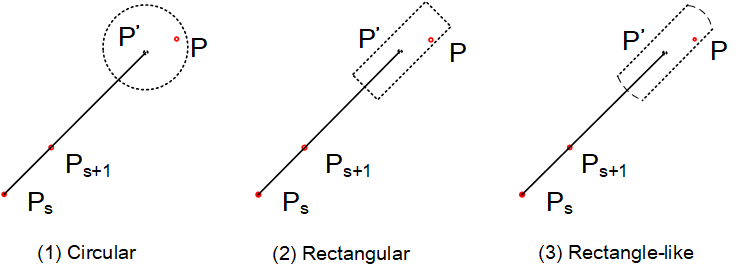
\includegraphics[scale=1.0]{Figures/Fig-Areas.png}\vspace{-1ex}
	%\caption{\small A trajectory is simplified by algorithm \dpa using distance metrics \ped, \sed and \dad, respectively.}
	\vspace{-1ex}
	\caption{\small Trajectory tracking in (1) a floating disc, (2) an infinite beam \cite{Chen:Space,Daescu:metric} and (3) a floating finite beam. Where $P_s$ is the start position of the sub-trajectory and $P'$ is the expected position of the moving object at time $P.t$ whose actually position at that time is $P$.}
	\vspace{-3ex}
	\label{fig:areas}
\end{figure}

\stitle{{Contributions}.}
To the end, we explore ways to track a moving object in a disc, an infinite beam and a finite beam, respectively, and design novel one-pass trajectory tracking algorithms that effectively and efficiently run for such areas. 

\ni (1) We develop a one-pass trajectory tracking algorithm \citt and theoretically prove that it has better effectiveness than \ldrh. Thus, we are able to effectively and efficiently track a moving object inside a floating disc (Section \ref{sec:circle}).
%\citt is more effective than \ldrh, great more efficient and a bit more effective than \grts (Section \ref{sec:circle}).

%\ni (2) We develop a one-pass trajectory tracking algorithm \sitt based on the intersection of sectors that tracks a moving object in a strip area. \sitt is the first algorithm that tracks a moving in a strip area, and is as concise and efficient as \citt (Section \ref{sec:strip}). %, and has a better compression ratio than \citt with a cost of a poorer accuracy.

\ni (2) We provide a convenient way to design new tracking shapes, \ie  an infinite and a finite beams, and develop novel one-pass trajectory tracking algorithms \sitt and \bitt such that we are able to effectively and efficiently track moving objects inside infinite and floating finite beams, respectively (Section \ref{sec:rectangle}). 
%\bitt is the first algorithm that tracks a moving object in a rectangle-like area, and it takes the advantages of both \citt and \sitt (Section \ref{sec:rectangle}). 
%\ie~\sitt based on the intersection of sectors that tracks a moving object in a strip area

\ni (3) Using three real-life trajectory datasets (Mopsi, SerCar, GeoLife), we finally conduct an extensive experimental study that compares our methods \citt and \bitt with representative trajectory tracking algorithms \ldrh (the first and the most efficient trajectory tracking algorithm) and \grts (the most effective trajectory tracking algorithm). The experimental results show that \citt and \bitt are both efficient and effective, and are feasible to track a moving object inside a disc and a beam, respectively (Section \ref{sec-exp}).


\eat{%%%%%%%%%%%%%%%%
\stitle{{Organization}}.
The remainder of the paper is organized as follows:
Section \ref{sec-pre} introduces the basic concepts and the \ldr and \ldrh approaches,
Sections \ref{sec:circle}, \ref{sec:strip} and \ref{sec:rectangle} present three one-pass algorithms that track in circular, strip and rectangle-like areas, respectively,
Section \ref{sec-exp} reports the experimental results of these methods, followed by related works in Section \ref{sec-related} and conclusion in Section \ref{sec-conclusion}.
All proofs are provided in the Appendix.
}%%%%%%%%%%%%%%%%eat




%%% Local Variables:
%%% mode: latex
%%% TeX-master: "gis18"
%%% End:



\section{Preliminaries}
\label{sec-pre}

In this section, we first introduce some basic concepts for trajectory tracking.
Then we introduce position and trajectory tracking algorithms \ldr and \ldrh that are helpful to understand the basic ideas of the work.
Notations used are summarized in Table \ref{tab:notations}.

\begin{table}
	\renewcommand{\arraystretch}{1.20}
	\caption{\small Summary of notations}
	\vspace{-1ex}
	\centering
	\footnotesize
	%\scriptsize
	\begin{tabular}{|c|l|}
		\hline
		{\bf Notations}& {\bf Semantics}   \\		\hline %\hline
		$P$ & a data point \\		\hline
		$\dddot{\mathcal{T}}$ & a trajectory $\dddot{\mathcal{T}}$ is a sequence of data points\\		\hline
		$\overline{\mathcal{T}}$&  {a piece-wise line representation of a trajectory $\dddot{\mathcal{T}}$}	\\		\hline
		$\mathcal{L}$ & a line segment  \\		\hline
		$\epsilon$ & an error bound \\		\hline
		$ped\left(P, \mathcal{L}\right)$ &  {the perpendicular Euclidean distance of point $P$ to line segment $\mathcal{L}$}	\\	\hline
		$sed\left(P, \mathcal{L}\right)$ & {the synchronous Euclidean distance of point $P$ to line segment $\mathcal{L}$} 	\\		\hline
		%$dad\left(\mathcal{L}_1, \mathcal{L}_2\right)$ & {the direction-aware distance of line segment $\mathcal{L}_1$ to line segment $\mathcal{L}_2$} 	%\\		\hline
		\sector{} & a sector \\		\hline
		%		$\overline{A} \times \overline{B}$ & the cross product of (vectors) $\overline{A}$ and $\overline{B}$\\		\hline
		%		$\mathcal{H}(\mathcal{L})$ & The open half-plane to the left of $\mathcal{L}$ \\		\hline
		%		$\mathcal{R}$& a convex polygon \\		\hline
		%		$\mathcal{R}^*$ & the intersection of convex polygons \\		\hline
		%		$m$ & the maximum number of edges of a polygon\\		\hline
		%		$E^j$ & a group of edges labeled with $j$\\		\hline
		%		$g(e)$ & the label of an edge $e$ of polygons \\		\hline
		%		\circle{} & a synchronous circle\\		\hline
		\cone{} & a spatio-temporal cone \\		\hline
		\circle{} & a synchronous circle \\		\hline
		%\pcircle{} & a cone projection circle \\		\hline
		$\mathcal{R}$& a convex polygon \\		\hline
		%$\mathcal{R}^*$ & the intersection of convex polygons \\		\hline
		%$\bigsqcap$ & intersection of geometries\\		\hline
		%$G$ &	the reachability graph of a trajectory\\		\hline
	\end{tabular}
	\label{tab:notations}
	\vspace{-1ex}
\end{table}


\begin{figure}[tb!]
	\centering
	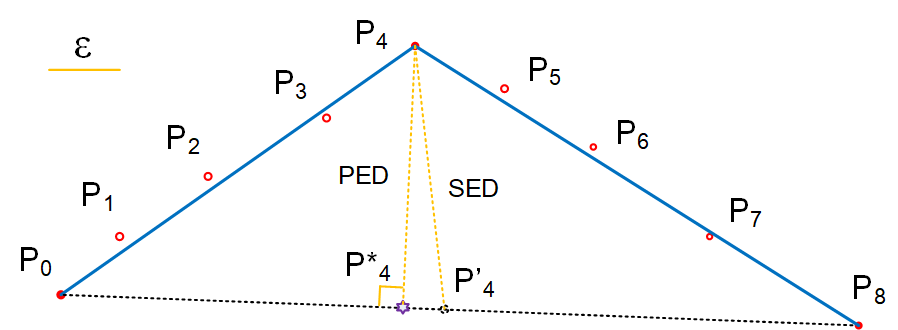
\includegraphics[scale=0.9]{Figures/Fig-Concepts.png}\vspace{-1ex}
	\caption{\small  A trajectory $\dddot{\mathcal{T}}[P_0, \ldots, P_{8}]$ with 9 points is simplified to (or represented by) two continuous line segments $ \overline{\mathcal{T}}[\overline{P_0P_4}, \overline{P_4P_{8}}] $ using \ped and \sed, respectively. In which, (1) $ped(P_4, \overline{P_0P_{8}})=|\overline{P_4P^*_4}|$, where $P^*_4$ is the perpendicular point of $P_4$ \wrt line segment $\overline{P_0P_{8}}$, and (2) $sed(P_4, \overline{P_0P_{8}})= |\overline{P_4P'_4}|$, where $P'_4$ is the synchronized point of $P_4$ \wrt $\overline{P_0P_{8}}$ satisfies ${|\overline{P_0P'_4}|}/{|\overline{P_0P_{8}}|} = \frac{(P_4.t - P_0.t)}{(P_{8}.t-P_0.t)} = \frac{(4-0)}{(8-0)}= \frac{1}{2}$.}
	\vspace{-1ex}
	\label{fig:concepts}
\end{figure}


\subsection{Notations}


%We first introduce basic notations.
\stitle{Trajectory}. A \textit{trajectory} $\dddot{\mathcal{T}}\left[P_0, \ldots, P_n\right]$ is a sequence of points in a monotonically increasing order of their associated time values (\ie $P_i.t < P_j.t$ for any $0\le i<j\le n$), where a data \textit{point} is defined as a triple $P\left(x, y, t\right)$, which represents that a moving object is located at {\em longitude} $x$ and {\em latitude} $y$ at {\em time} $t$. 
%Note that data points can be viewed as points in a three-dimension Euclidean space.


\eat{
	A \textit{line segment} (or line segment for simplicity) $\mathcal{L}$ is defined as $\overline{P_{s}P_{e}}$, which represents the closed line segment that connects the start point $P_s$ and the end point $P_e$.
	We also use $|\mathcal{L}|$ and $\mathcal{L}.\theta\in [0, 2\pi)$ to denote the length of a line segment $\mathcal{L}$, and its angle with the $x$-axis of the coordinate system $(x, y)$, where $x$ and $y$ are the longitude and latitude, respectively.
	That is, a line segment $\mathcal{L}$ = $\overline{P_{s}P_{e}}$ can be treated as a triple $(P_s, |\mathcal{L}|, \mathcal{L}.\theta)$.
}

%Intuitively, a trajectory can also be represented by a continuous $n$-pieces line segments (or line segment for simplicity) $\mathcal{L}_i$, $0\le i < n$, where  $\mathcal{L}_i = \overline{P_{i}P_{i+1}}$, represents the closed line segment that connects the start point $P_{i}$ and the end point $P_{i+1}$.

\stitle{Piece-wise line representation}. A \textit{piece-wise line representation} $\overline{\mathcal{T}}\left[\mathcal{L}_0, \ldots, \mathcal{L}_m\right]$ ($0< m \le n$) of a trajectory $\dddot{\mathcal{T}}\left[P_0, \ldots, P_n\right]$ is a sequence of continuous \textit{line segments} $\mathcal{L}_{i}$ = $\overline{P_{s_i}P_{e_i}}$ ($i\in\left[0,m\right]$) of $\dddot{\mathcal{T}}$ such that $\mathcal{L}_{0}.P_{s_0} = P_0$, $\mathcal{L}_{m}.P_{e_m} = P_n$ and  $\mathcal{L}_{i}.P_{e_i}$ = $\mathcal{L}_{i+1}.P_{s_{i+1}}$ for all $i\in\left[0, m-1\right]$.
Note that each line segment in $\overline{\mathcal{T}}$ essentially represents a continuous sequence of data points in trajectory $\dddot{\mathcal{T}}$.



For trajectory simplification, two Euclidean distance metrics are commonly used, namely, the \emph{perpendicular Euclidean distance} (\ped) and the \emph{synchronous Euclidean distance} \cite{Meratnia:Spatiotemporal} (\sed). Among them, \sed is also used in position and trajectory tracking.
%
Consider a data point $P$ and a line segment $\mathcal{L}$ = $\overline{P_{s}P_{e}}$.

\stitle{Perpendicular Euclidean distance}. The perpendicular Euclidean distance $ped\left(P, \mathcal{L}\right)$ of point $P$ to line segment $\mathcal{L}$ is $\min\{|PQ|\}$ for any point $Q$ on $\overline{P_{s}P_{e}}$.

\stitle{Synchronous Euclidean distance}. The synchronous Euclidean distance $sed\left(P, \mathcal{L}\right)$ of point $P$ to line segment $\mathcal{L}$ is $|\overline{PP'}|$ that is the Euclidean distance from $P$ to its \textit{synchronized point} $P'$ \wrt $\mathcal{L}$, where the synchronized point $P'$ \wrt $\mathcal{L}$ is defined as follows:
(a) $P'.x$ = $P_s.x +  c\cdot\left(P_e.x - P_s.x\right)$,
(b) $P'.y$ = $P_s.y +  c\cdot\left(P_e.y - P_s.y\right)$ and
(c) $P'.t$ = $P.t$, where $c= \frac{P.t-P_s.t}{P_e.t-P_s.t}$.

The \emph{synchronized point} $P'$ of a point $P$ \wrt line segment $\overline{P_sP_e}$ is the expected position of the moving object on $\overline{P_sP_e}$ at time $P.t$, obtained by a linear interpolation \cite{Cao:Spatio} that assumes it moved along the straight line from $P_s$ to $P_e$ with a uniform speed of $\frac{|\overline{P_sP_e}|}{P_e.t-P_s.t}$.


%Synchronized points are essentially virtual points with the assumption that an object moved along a straight line from $P_s$ to $P_e$ with a uniform speed, \ie the average speed $\frac{|\overline{P_sP_e}|}{P_e.t-P_s.t}$ between points $P_s$ and $P_e$ \cite{Cao:Spatio,Lin:Cised}. 

%More specifically, a synchronized point $P'_i$ of $P_i$ ($s\le i < e$) \wrt the line segment $\overline{P_sP_e}$ is a point on $\overline{P_sP_{e}}$ satisfying ${|\overline{P_sP'_i}|} = \frac{P_i.t - P_s.t}{P_e.t - P_s.t}\cdot {|\overline{P_sP_e}|}$, which means that the object moves from $P_s$ to $P_e$ at an average speed $\frac{|\overline{P_sP_e}|}{P_e.t-P_s.t}$, and its position at time $P_i.t$ is the point $P'_i$ on $\overrightarrow{P_sP_{e}}$ having a distance of $\frac{P_i.t - P_s.t}{P_e.t - P_s.t}\cdot|\overline{P_sP_e}|$ to $P_s$~\cite{Cao:Spatio, Lin:Cised,Meratnia:Spatiotemporal, Chen:Fast, Zhang:Evaluation}.


We illustrate these notations with examples shown in {Figure}~\ref{fig:concepts}.



 
 


\eat{%%%%%%%%%%%%%%
\begin{example}
	\label{exm-notations}
	Consider {Figure}~\ref{fig:concepts}, in which
	%
	(1) $\dddot{\mathcal{T}}\left[P_0, \ldots, P_{8}\right]$ is a trajectory having 9 data points,
	%
	(2) a set of two continuous line segments $\{\overline{P_0P_4}$, $\overline{P_4P_{8}}$\} is a piece-wise line representation of trajectory $\dddot{\mathcal{T}}$,
	%
	(3) $ped\left(P_4, \overline{P_0P_{8}}\right)=|\overline{P_4P^*_4}|$, where $P^*_4$ is the perpendicular point of $P_4$ \wrt line segment $\overline{P_0P_{8}}$, and 
	%
	(4) $sed\left(P_4, \overline{P_0P_{8}}\right)= |\overline{P_4P'_4}|$,
	where $P'_4$ is the synchronized point of $P_4$ \wrt $\overline{P_0P_{8}}$ satisfies $\frac{|\overline{P_0P'_4}|}{|\overline{P_0P_{8}}|} = \frac{P_4.t - P_0.t}{P_{8}.t-P_0.t} = \frac{4-0}{8-0}= \frac{1}{2}$.
\end{example}
}%%%%%%%%%%%%eat

\eat{%%%%%%%%%%%%%%%%%%
\stitle{Direction-aware distance distance}.The direction-aware distance $dad\left(\mathcal{L}_1, \mathcal{L}_2\right)$ is the direction deviation from $\mathcal{L}_1$ to $\mathcal{L}_2$, \ie $\Delta\left(\mathcal{L}_1.\theta, \mathcal{L}_2.\theta\right) = \min\{|\mathcal{L}_1.\theta - \mathcal{L}_2.\theta|, 2\pi - |\mathcal{L}_1.\theta - \mathcal{L}_2.\theta|\}$, where $\theta \in \left[0, 2\pi\right)$ is the angular of $\mathcal{L}$.
\textcolor{blue}{Note \dad differs from \ped and \sed in that it is a measure of angle, rather than Euclidean distances, and the temporal information is also lost when using \dad.}

\stitle{Trajectory simplification (Min-$\#$ problem).}
Given a trajectory \trajec{T}$\left[P_0, \dots, P_n\right]$ and a pre-specified constant $\epsilon$, the \emph{min-$\#$} problem of trajectory simplification is to approximate the trajectory \trajec{T} with $\overline{\mathcal{T}}\left[\mathcal{L}_0, \ldots , \mathcal{L}_m\right]$ ($0< m \le n$), such that
(1) on each of them the points $\left[P_{s_i}, \dots, P_{e_i}\right]$ are approximated by a line segment $\mathcal{L}_i = \overline{P_{s_i}P_{e_i}}$ with the maximum \ped or \sed \emph{error} of point $P_j$ (or \dad \emph{error} of line segment $|\overline{P_jP_{j+1}}|$) to line segment $\mathcal{L}_i$, $s_i \le j<e_i$,  less than $\epsilon$, and
(2) $P_{s_i}$ and $P_{e_i} \in$ \trajec{T}.


\stitle{Position tracking}. \textcolor{blue}{Given an error bound $\epsilon$, the position tracking is an agreement between a moving object and a MOD server such that the MOD server can infer the current position of the object with an deviation less than $\epsilon$ to its actual position.}

\stitle{Trajectory tracking}. It is a method implementing both trajectory simplification and position tracking.
}%%%%%%%%%%End EAT

\subsection{Position tracking in a circular area}

\textit{Position tracking} aims at informing the MOD about the current position of an object. Currently, the most simple yet efficient position tracking protocols is linear dead reckoning (\ldr) \cite{ Wolfson:PositionTracking}, which is essentially an agreement between a given moving object and the MOD server whose purpose is to let the MOD server track a moving object with less communication between them at an expense of imprecise of position within an error bound $\epsilon$.  

Given an error bound $\epsilon$, the moving object sends its initial location $P_s$ and the expected velocity $\vv{v}$
(including value and direction) to the MOD server, meaning that it is supposed to move from $P_s$ along the direction of $\vv{v}$ at a speed of $|\vv{v}|$, such that the expected position (\ie synchronized point) of the object at time $t>t_s$ can be extrapolated from them as long as no subsequent update is sent to the MOD server. 
After that, because the actual speed of it may be varied and different from the supposed speed of $|\vv{v}|$, the moving object periodically collects its actual position by sampling its on-board sensor, \eg GPS, and compares the actual position of time $t$ with the expected position of time $t$ extrapolated from the initial position $P_s$ and the velocity $\vv{v}$. 
If the deviation from its actual position to the expected position (\ie the synchronous Euclidean distance) is not more than $\epsilon$, then the object does not transmit any new updates to MOD, otherwise, an update of new ($P_s$, $\vv{v}$) will be sent.
%
By this way, though the MOD server receives less position information about a moving object, it still knows the expected position of the moving object with a bounded error of $\epsilon$ to its actual position. The \ldr mechanism ensures that no message is sent as long as the actual position $P$ is in the circular area around the excepted position $P'$ with a radius of $\epsilon$. That is, \emph{\ldr tracks a moving object in a floating circle having a velocity of $\vv{v}$.}

\begin{figure}[tb!]
	\centering
	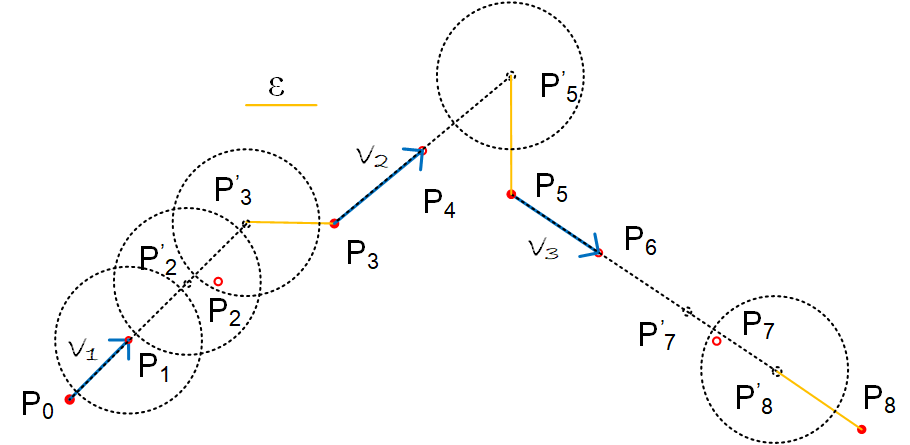
\includegraphics[scale=0.9]{figures/Fig-LDR.png}
	\vspace{-1ex}
	\caption{\small A running example of position tracking by \ldr. }
	\vspace{-1.5ex}
	\label{fig:ldr}
\end{figure}

\begin{example}
	\label{exm-ldr}
Figure \ref{fig:ldr} is a running example of \ldr.
Initially, point $P_0$ is set as $P_s$ and $\vec{v}$ is set to $\vec{v}_0$. Then, (1) points $P_1$ and $P_2$ have \sed distances less than $\epsilon$ to their expected points $P'_1$ and $P'_2$, respectively, and (2) $|P_3P'_3| > \epsilon$, meaning $P_3$ breaks the distance threshold, thus, a new update is triggered and $P_3$ is the new start point of the next section of position tracking.
%
\end{example}

%This example also demonstrates that (1) the expected position is indeed the synchronized point of the moving object at time $t$, (2) the deviation from the actual position to the expected position \wrt $\vv{v}$ is sure the synchronous Euclidean distance (\sed), and (3) 

 




\subsection{Trajectory tracking in a circular area}
\textit{Trajectory tracking} aims to implement both position tracking and trajectory simplification in one routine \cite{Lange:Tracking}. Currently, the one-pass trajectory tracking algorithm is a variation of \ldr, originally developed in \cite{Trajcevski:LDRH} and formally named as linear dead reckoning with half $\epsilon$ (\ldrh) in \cite{Lange:Tracking}.
%
Authors in \cite{Trajcevski:LDRH} proved that \ldr with some small variations is also a line simplification algorithm. Thus, \ldrh supports both position tracking and trajectory simplification, meaning it is a trajectory tracking algorithm.

Given an error bound $\epsilon$, \ldrh runs the same routine as \ldr except that (1) it uses half $\epsilon$ as the threshold in distance checking; (2) when the current point $P_k$ has a \sed larger than $\epsilon/2$ to its expected location (synchronous data point), it sends the preview point $P_{k-1}$ and a new $\vv{v}$ to the MOD server and continues trajectory tracking taking $P_{k-1}$ as the new start point. \ldrh is simple and efficient, having a linear time and a constant space. However, it has a poor effectiveness in terms of compression ratio, as the half $\epsilon$ is conservative, and more important, the algorithm is sensitive to the initial velocity which is set at the updating time but it is hard to be appropriate when the process goes on.

\begin{example}
Figure~\ref{fig:ldrh} is a running example of \ldrh taking the same input as Figure \ref{fig:ldr}.
Initially, the start point $P_s$ is set to $P_0$ and the velocity $\vec{v}$ is set to $\vec{v}_0$. Then, (1) $P_1$ and $P_2$ have \sed distances less than $\epsilon/2$ to their expected points $P'_1$ and $P'_2$, respectively, (2) $|P_3P'_3| > \epsilon/2$, thus, a new update is triggered and $P_2$ is the new start point of the next section of trajectory tracking. Finally, this algorithm in turn sends 5 points, $P_0, P_2, P_4, P_6$ and $P_8$, and 4 velocities, $\vec{v_1}$, $\vec{v_2}$, $\vec{v_3}$ and $\vec{v_4}$, to the MOD server.
\end{example}

\begin{figure}[tb!]
	\centering
	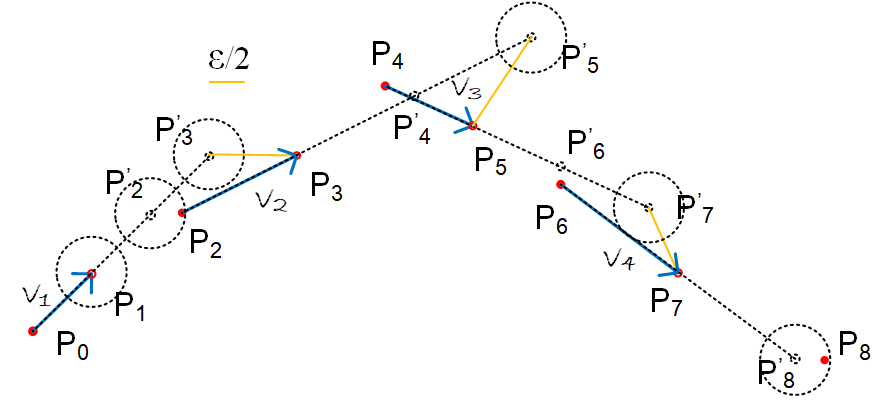
\includegraphics[scale=1.0]{figures/Fig-LDRH.png}
	\vspace{-1.5ex}
	\caption{\small A running example of trajectory tracking by \ldrh. }
	\vspace{-2ex}
	\label{fig:ldrh}
\end{figure}

%%%%%%
\eat{ 
	\textcolor{blue}{ 
		Lange et al. in \cite{Lange:GRTS, Lange:Tracking} introduced \grts framework that aimed at improving the effectiveness, in terms of compression ratio, of trajectory tracking by logically separating position tracking and trajectory simplification into two sub-processes, where position tracking is implemented by \ldr and trajectory simplification is enforced by integrating the third party line simplification algorithms \cite{Zhang:Evaluation, Lin:Cised}. \grts is effective than \ldrh, however, it is much more complex as it includes two sub-processes and introduces a buffer to temporarily save data points for the purpose of compression.
		Like \ldr, algorithms \ldrh and \grts both use \sed to check distances, hence, they also track a moving object in a floating circular area.}
}
%%%%%%eat







\subsection{Trajectory simplification based on spatio-temporal cones}

The recent trajectory simplification algorithm using \sed, namely \cised \cite{Lin:Cised}, is one-pass and also has a good effectiveness in terms of compression ratios. \cised uses a local synchronous distance checking approach based on a concept of \textit{spatio-temporal cone}, defined in a 3D Cartesian coordinate system whose $x$-axis, $y$-axis and $t$-axis are longitude, latitude and time, respectively, that converts the \sed distance tolerance into cones intersection for testing the successive points. This mechanism is potential to be extended for trajectory tracking with good effectiveness and efficiency.

\stitle{Spatio-temporal cone (\cone{}) \cite{Lin:Cised}}. 
Given a start point $P_s$ of sub-trajectory $\dddot{\mathcal{T}}_s[P_s, \ldots, P_{s+k}]$ and an error bound $\epsilon$, the spatio-temporal cone (or simply \textit{cone}) of a data point $P_{s+i}$ ($1\le i\le k$) in $\dddot{\mathcal{T}_s}$ \wrt $P_s$ and $\epsilon$, denoted as \cone{(P_s, P_{s+i}, \epsilon)}, or \cone{_{s+i}} in short, is an oblique circular cone such that point $P_s$ is its apex and the synchronous circle $\mathcal{O}(P_{s+i}, \epsilon)$ of point $P_{s+i}$, or \circle{_{s+i}} in short, a circle on the plane $P.t-P_{s+i}.t = 0$ such that $P_{s+i}$ is its center and $\epsilon$ is its radius, is its base (Figure~\ref{fig:cis}).

\eat{%%%%%%%%%%%
	\begin{example}
		\label{exm-circles-cones}
		Figure~\ref{fig:cis} shows 
		(1) two synchronous circles, \circle{(P_{s+i}, \epsilon)} of point $P_{s+i}$ and \circle{(P_{s+k}, \epsilon)} of point $P_{s+k}$.
		It is easy to see that for any point in the area of a circle \circle{(P_{s+i}, \epsilon)}, its distance to $P_{s+i}$ is not greater than $\epsilon$, 
		and (2) two example spatio-temporal cones, \cone{(P_s, P_{s+i}, \epsilon)} {(purple)} and \cone{(P_s, P_{s+k}, \epsilon)} (red), with the same apex $P_s$ and error bound $\epsilon$. %\eop
	\end{example}
}%%%%%%%%%%%

%Note that in this definition, a \emph{synchronous circle} $\mathcal{O}(P_i, \epsilon)$ is only defined by a central point $P_i$ and a constant $\epsilon$. Indeed, it is nothing to do with any start point $P_s$ or end point $P_e$.


%\textcolor{blue}{We define \textit{synchronous circles and Spatio-temporal cones} in a \emph{x-y-t} 3D coordinate system, and build the connection between \textit{synchronous circles} and \textit{synchronous distances}.}



\begin{figure}[tb!]
	\centering
	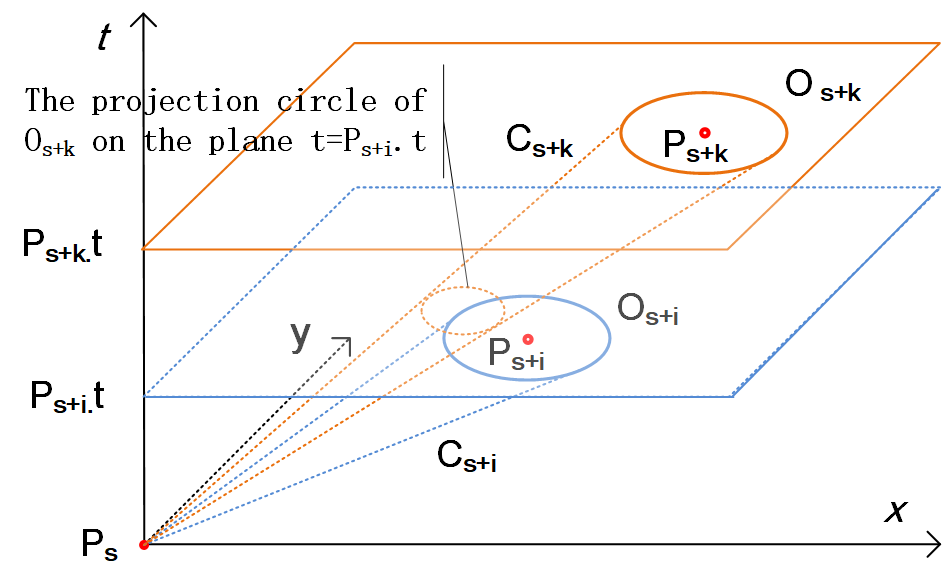
\includegraphics[scale=0.88]{figures/Fig-CIS.png}
	\vspace{-2ex}
	\caption{\small Examples of spatio-temporal cones in a 3D Cartesian coordinate system taking point $P_s$ as the origin, where (1) $P_{s+i}$ and $P_{s+k}$ are two points, (2) \circle{_{s+i}} and \circle{_{s+k}} are two synchronous circles, (3) \cone{_{s+i}} and \cone{_{s+k}} are two spatio-temporal cones.}
	\vspace{-1ex}
	\label{fig:cis}
\end{figure}
%, (4) $Q$ is a point in synchronous circle \circle{_{s+k}}, and (5) $P'_{s+i}$ is the intersection point of line $\protect\overline{P_sQ}$ and synchronous circle \circle{_{s+i}}

Based on the spatio-temporal cone, authors in \cite{Lin:Cised} prove that the \sed distance tolerance can be checked by finding the common intersection of spatio-temporal cones  (half-$\epsilon$) built from points of a sub-trajectory $[P_s,...,P_{s+k}]$, \ie ``{given a sub-trajectory $[P_s,...,P_{s+k}]$ and an error bound $\epsilon$, $sed(P_{s+i}, \overline{P_sP_{s+k}})\le \epsilon$ for each $i \in [1,k]$ if  $\bigsqcap_{i=1}^{k}$\cone{(P_s, P_{s+i}, \epsilon/2)} $\ne \{P_s\}$}."
In other words, if these cones do have a common intersection, then line segment $\overline{P_sP_{s+k}}$ can represent the sub-trajectory. And for efficiency consideration, \cised projects those cones on a plane, \eg plane $t=P_{s+1}.t$, so as to convert the checking of cones intersection into a much simpler way, \ie~\textit{checking of circles intersection on the plane} (Figure~\ref{fig:cis}).
For the same reason, a circle is further approximated by its inscribe regular polygon and the intersecting of circles is approximated by the intersecting of these polygons, which can be computed in linear time.
%
%Note that though the cone intersection approach outperform the counterpart of \ldr and \ldrh, it is still not introduced to trajectory tracking.

\eat{%%%%%%%%%%%%%%%%%% Delete because of the page limitation.
	Figure~\ref{fig:cised} is a running example of \cised. In this case, it outperforms \ldrh in terms of compression ratio.
	
	\begin{figure}[tb!]
		\centering
		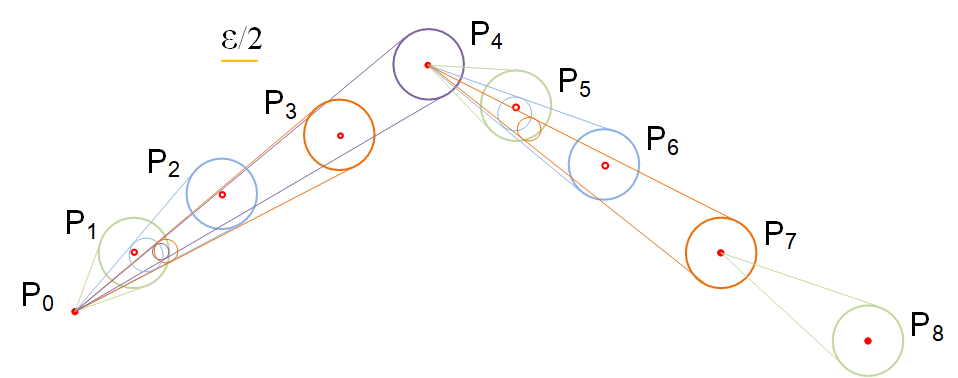
\includegraphics[scale=0.9]{figures/Fig-CISED-SH.png}
		\vspace{-1ex}
		\caption{\small A running example of \cised. In the first section, cones are projected on plane $P_1.t$, where (1) the projection circles of \circle{_{1}},\circle{_{2}},\circle{_{3}} and \circle{_{4}} have common intersection, and (2) it does not intersected with the projection circle of \circle{_{5}}. Thus, $P_4$ is output, and it serves as the new start point of the next section. Finally, the same trajectory is simplified to four points $\{P_0, P_4, P_7, P_8\}$.}
		\vspace{-2ex}
		\label{fig:cised}
	\end{figure}
}%%%%%%%%%%%%%%%%%%%%%%



%\subsection{Trajectory simplification in strip areas}
%\todo{sleeve (half-epsilon)}


\section{Effective and efficient tracking in a circular area}
%\section{Tracking in a circular area}
\label{sec:circle}

{\ldrh is a one-pass trajectory tracking algorithm, having linear time and constant space complexities, and suffering in effectiveness (compression ratios).
Observing the recently trajectory simplification algorithm \cised using \sed is also one-pass (which is important for a trajectory tracking algorithm that is supposed to run on mobile devices), and at the same time, it has a good effectiveness (compression ratios), these inspire us to develop an efficient and effective trajectory tracking algorithm using \sed.}


\subsection{Tracking by spatio-temporal cones}

In this section, we will first show that the counterpart of \ldrh is just a special case of, and has a worse effectiveness in terms of compression ratio than the approaches based on spatio-temporal cone (even it uses a half-$\epsilon$ cone), thus, the latter is obviously a more effective way to develop trajectory tracking algorithms. Then, we further extend the half-$\epsilon$ cone used in \cised to a full-$\epsilon$ cone so as to get an even better effectiveness.



\begin{theorem}
\label{theo-ldrh-cised}
Given a sub-trajectory $\dddot{\mathcal{T}}_s[P_s,...,P_{s+k}]$ and an error bound $\epsilon$, if $\dddot{\mathcal{T}}_s$ can be represented by line segment $\overline{P_sP_{s+k}}$ through algorithm \ldrh, then it can also be represented by approaches based on spatio-temporal cones.
\end{theorem}

Theorem \ref{theo-ldrh-cised} tells that (1) {approaches based on the spatio-temporal cone are also applicable to do trajectory tracking in a circular area}, and (2) \ldrh is just a special case of and has a worse effectiveness than approaches based on spatio-temporal cones. \ldrh assumes an initial velocity before the simplification or tracking of a sub-trajectory, while the spatio-temporal cone based methods do not, instead, it has an ability to find out the potentially feasible velocities to fit the movement of the object when it simplifies the sub-trajectory. Thus, the latter is sure a more effective way to develop one-pass trajectory tracking algorithms. 
%
Moreover, observe that the half-$\epsilon$ cone in the above is still a little conservative, we next extend it to a full-$\epsilon$ cone.% plus certain constrain to get an even better effectiveness.


\begin{theorem}
	\label{theo-full-cone}
	Given a sub-trajectory $[P_s,...,P_{s+k}]$ and an error bound $\epsilon$, $sed(P_{s+i}, \overline{P_sP_{s+k}})\le \epsilon$ for each $i \in [1,k]$ if $\overline{P_sP_{s+k}}$ passes through $\bigsqcap_{i=1}^{k-1}$\cone{(P_s, P_{s+i}, \epsilon)} - \{$P_s$\}.
\end{theorem}

Theorem \ref{theo-full-cone} tells that full-$\epsilon$ spatio-temporal cones, with a constrain that the line segment $\overline{P_sP_{s+i}}$ passes through the common intersection of all the preview cones, can also be used in trajectory simplification and/or tracking. Thus we get two ways of trajectory tracking in a circle. The question is, which one is the better?

\begin{theorem}
	\label{theo-cone-vs}
	Given a sub-trajectory $[P_s,...,P_{s+k}]$ and an error bound $\epsilon$, if $\bigsqcap_{i=1}^{k}$\cone{(P_s, P_{s+i}, \epsilon/2)} $\ne \{P_s\}$, then $\overline{P_sP_{s+k}}$ passes through $\bigsqcap_{i=1}^{k-1}$\cone{(P_s, P_{s+i}, \epsilon)}-$\{P_s\}$; and the opposite is not necessarily true.
\end{theorem}


Theorem \ref{theo-cone-vs} tells that, given the same sub-trajectory and start point, the full-$\epsilon$ cone approach has an ability to include more points into a line segment than the half-$\epsilon$ cone, which is in turn better than \ldrh, in trajectory simplification and/or tracking. Thus, it is better to use the full-$\epsilon$ cone to develop trajectory tracking algorithms.
%as shown in Proposition \ref{theo-ldrh-cised}

\subsection{Implementation}
We then provide a one-pass trajectory tracking algorithm based on spatio-temporal cone, named \underline{C}one \underline{I}ntersection for \underline{T}rajectory \underline{T}racking (\citt). This algorithm runs on mobile devices and uses full-$\epsilon$ spatio-temporal cones. In a nutshell, when a distance deviation of position tracking occurs, unlike \ldr and \ldrh, algorithm \citt does not roughly send an update of a new start position $P_s$ and a new velocity $\vv{v}$ to the MOD server. Instead, it quickly finds out a new feasible velocity $\vv{v}$ by the intersection of spatio-temporal cones such that only the new velocity $\vv{v}$ is sent to the MOD server while the start point $P_s$ keeps the same. By this way, a line segment clearly represents a longer sub-trajectory than \ldrh, and therefor the storage and network bandwidth are saved.

\stitle{Algorithm \citt}. Given a trajectory $\dddot{\mathcal{T}}$ and an error bound $\epsilon$, \citt initializes the velocity $\vv{v}$ (including value and direction) and sends it coupling with the start position $P_s$ of the trajectory to the MOD server. Then, for each point $P_{s+i}$, $i>0$, it checks (1) the deviation of the actual position $P_{s+i}$ to its synchronized point $P'_{s+i}$ built from the start point $P_s$, velocity $\vv{v}$ and time $P_{s+i}.t$, for the purpose of position tracking, and (2) the common intersection of spatio-temporal cones built from points $P_{s+j}$, $j \in [1, i]$, for the purpose of trajectory simplification.
%
During the checking, (1) if the common intersection of cones is $\{P_s\}$, then an update of new $(P_s, \vv{v})$ is sent to the MOD server and the algorithm goes on to process the next sub-trajectory start from the new $P_s$;
%
(2) if the common intersection is not $\{P_s\}$ but the position deviation is lager than the given threshold $\epsilon$, meaning this sub-trajectory can be represented by a line segment and there is a more appropriate velocity $\vv{v}$ for position tracking, then an update of the new $\vv{v}$ is sent to the MOD server and the algorithm goes on processing the same sub-trajectory start from the $P_s$;
%
otherwise, (3) no deviation occurs, no update is sent and the algorithm goes on processing the same sub-trajectory. 
%
When setting a new velocity $\vec{v}$, any $\vec{v}$ satisfying $\vec{v}.\theta = \overline{P_sQ}.\theta$ and $|\vec{v}|=|P_sQ|/(Q.t-P_s.t)$ is applicable, where $Q$ is a point living in the common intersection of the spatio-temporal cones. For convenience, we roughly let $Q$ be the current point $P_{s+i}$.

%Note that like \cised, this algorithm also transforms the intersection of cones to the intersection of regular polygons.

\begin{figure}[tb!]   % full cones
	\begin{center}
		{\small
			\begin{minipage}{3.3in}
				\myhrule
				%\vspace{-1ex}
				\mat{0ex}{
					{\bf Algorithm}~\citt $(\dddot{\mathcal{T}}[P_0,\ldots,P_n],~\epsilon,~m)$\\
					%	\sstab
					\bcc \hspace{1ex}\= $P_s := P_0$; ~~~~$\mathcal{R}^*$ := \kw{getRPolygon}($P_s$, $P_{s+1}$, $\epsilon$, $m$, $P_{s+1}.t$); \\
					\icc \hspace{1ex}\= $|\vv{v}|:=\frac{|P_{s}P_{s+1}|}{P_{s+1}.t-P_s.t}$; ~~~~$\vv{v}.\theta:=\overline{P_{s}P_{s+1}}.\theta$; \\
					\icc \hspace{1ex}\= update ($P_{s}, \vv{v}$); \\
					\icc \hspace{1ex}\= $i := 2$; 	\\
					\icc \hspace{1ex}\= while $i \le n$ do \\
					\icc \>\hspace{3ex} if $\overline{P_sP_{i}}$ ~does not pass~ $\mathcal{R}^*$ then \\ % // updates velocity and location \\
					\icc \>\hspace{7ex}    $P_s := P_{i-1}$; ~~~~$\mathcal{R}^*$ := $\emptyset$; \\
					\icc \>\hspace{7ex}    $|\vv{v}|:=\frac{|P_{s}P_{i}|}{P_{i}.t-P_s.t}$; ~~~~~$\vv{v}.\theta:=\overline{P_{s}P_{i}}.\theta$; \\
					\icc \>\hspace{7ex}    update ($P_{s}, \vv{v}$); \\
					\icc \>\hspace{3ex} else if $sed(P_{i},\vv{v}) \ge \epsilon $ then  \\ %~$\overline{P_sP_{i}}$ ~passes~ $\mathcal{R}^*$ and
					\icc \>\hspace{7ex}    $|\vv{v}|:=\frac{|P_sP_{i}|}{P_{i}.t-P_s.t}$; ~~~~~$\vv{v}.\theta:=\overline{P_sP_{i}}.\theta$; \\
					\icc \>\hspace{7ex}    update ($\vv{v}$); \\
					\icc \>\hspace{3ex} if $\mathcal{R}^*=\emptyset$ then $\mathcal{R}^*:=$ \kw{getRPolygon}($P_s$, $P_{i}$, $\epsilon$, $m$, $P_{s+1}.t$); \\
					\icc \>\hspace{3ex} else $\mathcal{R}^*$ := $\mathcal{R}^*\bigsqcap$ \kw{getRPolygon}($P_s$, $P_{i}$, $\epsilon$, $m$, $P_{s+1}.t$); \\
					\icc \>\hspace{3ex} $i$ := $i +1$;	\\
					\icc \>\hspace{0ex} update $(P_{n}, 0)$; 
				}
				\vspace{-2ex}
				\myhrule
			\end{minipage}
		}
	\end{center}
	\vspace{-2ex}
	\caption{\small Trajectory tracking based on spatio-temporal cone.}
	\label{alg:citt-s-full}
	\vspace{-2ex}
\end{figure}
%%%%%%%%%%%%%%%%%%%%%%%%%%%%%%%%%%%%%


Figure~\ref{alg:citt-s-full} is the P-codes of \citt. It takes as input a trajectory \trajec{T}${[P_0, \ldots, P_n]}$, an error bound $\epsilon$ and the number $m$ of edges for an inscribed regular polygon (recall in \cised, a circle is approximated by its $m$--edges inscribe regular polygon and accordingly the intersecting of circles is approximated by the intersecting of these polygons), and outputs a set of velocities and a simplified  trajectory $\overline{\mathcal{T}}$ of $\dddot{\mathcal{T}}$.
%
The algorithm first initializes the start point $P_s$ to $P_0$, the common intersection of polygons $\mathcal{R}^*$ to the regular inner polygon of $P_1$ by calling procedure $\kw{getRPolygon}()$ \cite{Lin:Cised}, and the expected velocity $(|\vv{v}|, \vv{v}.\theta)$ to ($\frac{|P_{s}P_{s+1}|}{P_{s+1}.t-P_s.t},\overline{P_{s}P_{s+1}}.\theta$) (lines 1--2), then it sends its initial location $P_s$ and the velocity $\vv{v}$ to the MOD server (line 3), meaning that it is supposed to move from point $P_s$ along the direction of $\vv{v}.\theta$ at a speed of $|\vv{v}|$.
%, such that the expecting position of the object at time $t>P_s.t$ can be extrapolated from them as long as no subsequent update is sent to the MOD server.
%
This algorithm sequentially processes the rest points of the trajectory one by one (lines 4--15). 
For the current point $P_{i}$, if $\overline{P_sP_{i}}$ passes through the common intersection $\mathcal{R}^*$, meaning that it can not includes more points into a line segment, then a line segment $\overline{P_sP_{i-1}}$ and a new section started from  $P_{i-1}$ is generated, the common intersection of cones is set to null, and $P_{i-1}$ and a new velocity $\vv{v}$ are sent to the MOD server (lines 6--9).
%
Otherwise, it calculates the distance from the actual location $P_{i}$ to the expecting location $P'_{i}$ extrapolated from the initial location $P_s$ and the velocity $\vv{v}$, and checks whether $\overline{P_sP_{i}}$ passes through the common intersection $\mathcal{R}^*$ of the preview points.
If it passes through and the distance $|P_{i}P'_{i}| \ge \epsilon$, meaning that more points can be included into a line segment while the velocity $\vv{v}$ needs to be updated. Hence, it updates velocity $\vv{v}$ based on $P_s$ and $P_{i}$, and sends it to the MOD server (lines 10--12). 
%
Anyway, the algorithm gets the $m$-edge inscribed regular polygon \wrt the current point $P_{i}$ by calling procedure $\kw{getRPolygon()}$ \cite{Lin:Cised} and gets the common intersection $\mathcal{R}^*$ of the preview cones (lines 13--14). The process repeats until all points have been processed (line 15).
At last, it outputs the last point $P_{n}$ (line 16).
%





\begin{figure}[tb!]
	\centering
	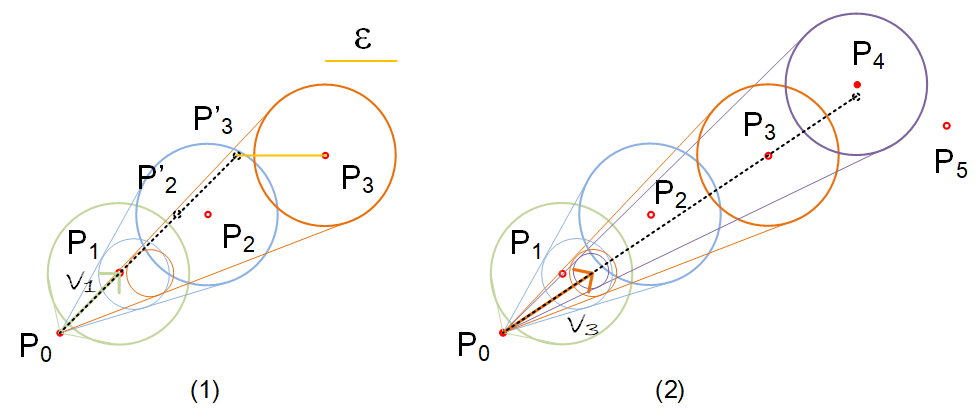
\includegraphics[scale=1.0]{figures/Fig-CITT.png}
	\vspace{-2ex}
	\caption{\small A running example of trajectory tracking by \citt. }
	\vspace{-3ex}
	\label{fig:citt}
\end{figure}


\begin{example}
	Figure~\ref{fig:citt} is a running example of algorithm \citt. It takes the same input and sets the same start point and initial velocity as Figure~\ref{fig:ldr}, and uses full-$\epsilon$ cones to simplify the trajectory. Then, (1) $P_3$ lives in the common intersection of \cone{_{1}} and \cone{_{2}} and it has a distance larger than $\epsilon$ to its expected position $P'_3$ \wrt $\vec{v_1}$, thus, \citt updates the velocity from $\vec{v_1}$ to $\vec{v_3}$ and the process goes on, and (2) $P_5$ is outside of the common intersection of the preview cones, thus, $P_4$ serves as the new start point, and an update is triggered. Finally, this algorithm sends three points, $P_0, P_4$ and $P_8$ (not shown), and four velocities, $\vec{v_1}$, $\vec{v_3}$, $\vec{v_5}$ (not shown) and $\vec{v_8}$ (not shown), to the MOD server. Also note that, no matter during the tracking or after the simplification, this algorithm ensures that any removed point is located in a circle around its expected position \wrt a velocity of trajectory tracking or a line segment connecting two neighboring data points of the simplified trajectory. 
\end{example}


\stitle{Correctness and complexity.} 
The correctness of algorithm \citt follows from Theorems \ref{theo-ldrh-cised} and \ref{theo-full-cone}.
It is easy to find that every point is processed only once in \citt, and for each point, it needs $O(1)$ time as getRPolygon() \cite{Lin:Cised}, intersecting of polygons \cite{Lin:Cised} and {other operations} all have a time complexity of $O(1)$. Hence, \citt has a time complexity of $O(n)$, where $n$ is the number of data points.






\eat{%%%%%%%%%%%%%%%%%%%%%%%%%%%%%%%%%%%%%%%%%%%%%%%%
	
\subsection{Weak tracking}

-- theorem: if ldr is true, then the intersection of those cones must not be \{$P_s$\}.
means that, if ldr is true, it is sure those points can be represented by a line segment.
thus, we only need to check the intersection after ldr is false, during the process.

-- algorithm CITT-W(e)

-- example

-- correctness and complexity
}%%%%%%%%%%%%%%%%%%%%%%%%%%%%%%%%%%%%%%%%%%%%%%%%%%%%%

%
%%% Local Variables:
%%% mode: latex
%%% TeX-master: "www2019"
%%% End:

\section{Tracking in a strip area}
\label{sec:strip}




%\subsection{Position tracking in strip areas}
%based on ldr, a direction is needed, no speed;
%  --  distance checking during computing, ped: from a point to a ray.
  

\subsection{\ped, sector and trajectory simplification}
\label{sec:sector-in-simp}



\subsection{Tracking by sectors}



\subsection{Implementation}

We then present a one-pass trajectory tracking algorithm based on full-$\epsilon$ sector, named \underline{S}ector \underline{I}ntersection for \underline{T}rajectory \underline{T}racking (\sitt). As shown in Figure ~\ref{alg:sitt}, \sitt runs in a similar routine as \citt excepts that (1) \sed and spatio-temporal cone are replaces by \ped and sector, (2) only the direction information of $\vv{v}$ is needed while the speed information is not, such that when a distance deviation occurs, \sitt quickly finds out a new feasible direction of velocity $\vv{v}$ by the intersection of sectors and sends it to the MOD server, and (3) it temporarily saves the maximum length of $|P_sP_{s+j}|$, $j\in (0, i)$, in $l_m$ and compares it with the length $|P_sP_{s+i}|$ of the current point $P_{s+i}$ during the process, as mentioned in Theorem \ref{theo-full-sector}. 
%
During tracking, the moving object is in a strip around the velocity. And after simplification, those removed points are located in $2\epsilon$--width strips around those saved points.





\stitle{Correctness and complexity.} 
The correctness of algorithm \sitt follows from Theorems \ref{theo-half-sector} and \ref{theo-full-sector}.
It is also easy to find that every point is processed only once in \sitt, and for each point, it needs $O(1)$ time as getSector() \cite{Zhao:Sleeve}, intersecting of sectors \cite{Zhao:Sleeve} and {other operations} all have a time complexity of $O(1)$. Hence, \sitt has a time complexity of $O(n)$, where $n$ is the number of data points.





%%% Local Variables:
%%% mode: latex
%%% TeX-master: "www2019"
%%% End:

\section{Tracking in a rectangle-like area}
\label{sec:rectangle}
Currently, position tracking and trajectory tracking methods both use \sed as the distance metric to check data points and confirm the actual position of a moving object at time $t$ lives in a circle around the excepting position of the moving object at that time.
{However, as mentioned in Section~\ref{sec-intro}, there is a need of tracking a moving object in other areas, \ie a strip or rectangular area.}
Note that, though it is possible to track a moving object in a rectangular area, it is really hard to design such a shape without introducing a new distance metric other than the well-known metrics \sed and \ped, and at the same time develop an efficient algorithm for that.
Alternatively, this section defines a rectangle-like area that subtly makes use of \ped and \sed, and then develops such an effective and efficient trajectory tracking algorithm.
%, and (2) a circular or strip area is indeed a special case of a rectangle-like area.
%as in \cite{Lin:Dual}, 

\subsection{Building the rectangle-like areas}

Like the circular area related to \sed, a rectangle-like area is also related to a Euclidean distance metric, namely the binary Euclidean distances of \sed and \ped.


\stitle{Binary Euclidean distances of \sed and \ped}, shortly \bed (\sed, \ped), is the combination of distance metrics \sed and \ped where their error bounds are set separately to $\epsilon_{sed}$ and $\epsilon_{ped}$, such that (1) if $\epsilon_{ped} \ge \epsilon_{sed}$, then it falls back to the \sed, \ie tracking in a circular area, as shown in {Figure~\ref{fig:areas}-(1)};
%
(2) if $\epsilon_{ped} << \epsilon_{sed}$, then its effect is actually approximate to a \ped, which is familiar in trajectory simplification, but not seemed in position and trajectory tracking, that always ensures that the original data points live in strip-like areas built around the simplified trajectory, as shown in {Figure~\ref{fig:areas}-(2). Otherwise, 
%
(3) it is the double effects of \ped and \sed, and forms a rectangle-like shape whose short sides are replaced by circular arcs of \sed as shown in {Figure~\ref{fig:areas}-(3)}. 


The shape of a rectangle-like area is controlled by two independent parameters, $\epsilon_{ped}$ and $\epsilon_{sed}$, thus, by carefully setting them, we not only build such rectangle-line areas that satisfy the needs of varied applications but also balance two performance metrics, the compression ratios and the errors of spatio-temporal queries, of trajectory simplification/tracking algorithms. 
%For the same example of ``the school boy on his way home'' mentioned in Section \ref{sec-intro}, if we only use \ped with a fixed ``$\epsilon$'', then we get a simplified trajectory having a good compression ratio and a unbounded query error; if we only use \sed with the same ``$\epsilon$'', then we get a poorer compression ratio and a bounded query error. However, if we combine them, \ie~use the \bed, then we could get a medium compression ratio and a bounded query error.


%


\eat{ %%%%%%%%%%%%%%
Given a sequence of points $[P_{s}, P_{s+1}, \ldots, P_{s+k}]$ and an error bound $\epsilon$,
for the start data point $P_s$, any point $P_{s+i}$ and $|\overline{P_sP_{s+i}}|>\epsilon$ ($i\in[1, k]$), there are two directed lines $\overline{P_sP^u_{s+i}}$ and $\overline{P_sP^l_{s+i}}$ such that $ped(P_{s+i}, \overline{P_sP^u_{s+i}})$ $=$ $ped(P_{s+i}, \overline{P_sP^l_{s+i}}) = \epsilon$ and either ($\overline{P_sP^l_{s+i}}.\theta < \overline{P_sP^u_{s+i}}.\theta ~and~\overline{P_sP^u_{s+i}}.\theta - \overline{P_sP^l_{s+i}}.\theta <\pi$) or ($\overline{P_sP^l_{s+i}}.\theta > \overline{P_sP^u_{s+i}}.\theta ~and~ \overline{P_sP^u_{s+i}}.\theta - \overline{P_sP^l_{s+i}}.\theta < -\pi)$. Indeed, they form a \emph{sector} \sector{(P_s, P_{s+i}, \epsilon)} that takes $P_s$ as the center point and $\overline{P_sP^u_{s+i}}$ and $\overline{P_sP^l_{s+i}}$ as the borderlines (Figure~\ref{fig:sleeve}-(1)).
%
Then, like the checking of the common intersection of spatio-temporal cones in \cised, these sector-based algorithms check the common intersection of sectors, \ie $\bigsqcap_{i=1}^{k}$\sector{(P_s, P_{s+i}, \epsilon)} $\ne \{P_s\}$ \cite{Williams:Longest, Sklansky:Cone,Zhao:Sleeve}, to find out whether the sub-trajectory can be represented by a line segment $\overline{P_sQ}$ \wrt error bound $\epsilon$, where $Q$ is a point that may not belong to the sub-trajectory. However, if $Q$ must be $P_{s+k}$, the last point of the sub-trajectory, \eg $P_3$ in Figure~\ref{fig:sleeve}-(2), then (1) the full-$\epsilon$ sectors should be replaced by half-$\epsilon$ sectors, and (2) $P_{s+k}$ should be one of the points having the furthest distances to $P_s$, \ie $|P_sP_{s+k}| \ge l_{m}$, where $l_{m}=max\{|P_sP_{s+i}|\}$~for each $i \in (0, k)$. 
}%eaten

\begin{figure}[tb!]
	\centering
	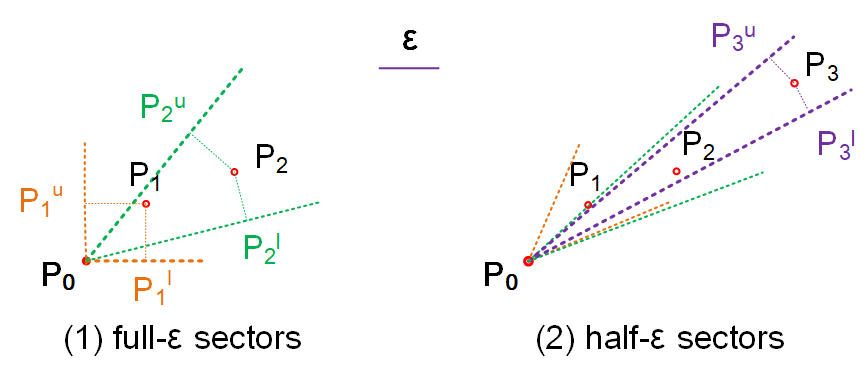
\includegraphics[scale=1.0]{figures/Fig-Sleeve.png}
	\vspace{-2ex}
	\caption{\small Examples of sectors and their intersection.}
	\vspace{-2ex}
	\label{fig:sleeve}
\end{figure}


\subsection{Tracking with cones and sectors}


%\ped is familiar in trajectory simplification, where an error-bounded algorithm using \ped always ensures that the original data points live in strip-like areas built from the simplified trajectory. 
%Though \ped is not seemed in position and trajectory tracking, indeed, the sector built from \ped is applicable to track a moving object in a strip area, like the spatio-temporal cone built from \sed that is used to track trajectory in a circular area.


First, similar as the spatio-temporal cones built from \sed are used in simplifying trajectory in circular areas, a mechanism based on sectors built from \ped is used to simplify trajectory in strip areas. Here, a \emph{sector} is largely a simplified version of a spatio-temporal cone projected on an $x$--$y$ 2D space that the temporal information is ignored, that converts the \ped distance tolerance into an angle tolerance for efficiently checking the successive data points. 
Then \textit{sector intersection} \cite{Williams:Longest, Sklansky:Cone, Dunham:Cone, Zhao:Sleeve}, originally developed in fields of computational geometry and cartography to efficient simplifies the border lines of a geometric or cartographic shape in digital format, is an efficient and effective way to simplify trajectories as pointed out in \cite{Lin:Cised}.
We next demonstrate that it is also applicable to track trajectory in strip areas.


\begin{theorem}
	\label{theo-half-sector}
	Given a sub-trajectory $[P_s,...,P_{s+k}]$ and an error bound $\epsilon$, the trajectory can be tracked in a strip area by an approach based on the intersection of sectors.
\end{theorem}

Because the half-$\epsilon$ sector approach of \cite{Williams:Longest, Sklansky:Cone,Zhao:Sleeve} may limit the performance of compression ratio, we also extend it to full-$\epsilon$ sectors for better performance.

\begin{theorem}
	\label{theo-full-sector}
	Given a sub-trajectory $[P_s,...,P_{s+k}]$ and an error bound $\epsilon$, $ped(P_{s+i}, \overline{P_sP_{s+k}})\le \epsilon$ for each $i \in [1,k]$ if line segment $\overline{P_sP_{s+k}}$ passes through $\bigsqcap_{i=1}^{k-1}$\sector{(P_s, P_{s+i}, \epsilon)} - \{$P_s$\} ~and~ $|P_sP_{s+k}| \ge \sqrt{l_{m}^2 - \epsilon^2}$, where $l_{m} = max\{|P_sP_{s+i}|\}$ for each $i \in (0, k)$.
\end{theorem}

Theorem \ref{theo-full-sector} tells that full-$\epsilon$ sector approach with constrains that (1) $\overline{P_sP_{s+k}}$ lives in the common intersection of the preview full-$\epsilon$ sectors and (2) $|P_sP_{s+k}|$ is longer than $\sqrt{l_{m}^2 -\epsilon^2}$, is applicable to simplify and track a moving object in a strip area. Because the full-$\epsilon$ sector and $|P_sP_{s+k}| \ge \sqrt{l_{m}^2 - \epsilon^2}$ are looser constraints than the half-$\epsilon$ sector and $|P_sP_{s+k}| \ge l_{m}$ used in \cite{Williams:Longest, Sklansky:Cone,Zhao:Sleeve}, this new approach is sure of bringing a better compression ratio.

\eat{%%%%%%%%%%%%%%%%%%%
	\begin{theorem}
		\label{theo-sector-vs}
		Given a sub-trajectory $[P_s,...,P_{s+k}]$ and an error bound $\epsilon$, if $\bigsqcap_{i=1}^{k}$\sector{(P_s, P_{s+i}, \epsilon/2)} $\ne \{P_s\}$, then $\overline{P_sP_{s+k}}$ passes through $\bigsqcap_{i=1}^{k-1}$\sector{(P_s, P_{s+i}, \epsilon)}-$\{P_s\}$; and the opposite is not necessarily true.
	\end{theorem}
	
	
	Theorem \ref{theo-sector-vs} tells that the full-$\epsilon$ sector approach also brings a better effectiveness than the half-$\epsilon$ sector, hence it is the dominant way to develop trajectory simplification/tracking algorithms.
}%%%%%%%%%%%%%%%%%%%%%%%%





%\myblue{Is there an effective and efficient trajectory algorithm implementing \bed that tracks a moving object in a rectangle-like area? Theorem \ref{theo-binary} is the answer to this question.}
Second, by combining cones and sectors, we are able to efficiently track trajectory in rectangle-like areas.

\begin{theorem}
	\label{theo-binary}
	Given a sub-trajectory $[P_s,...,P_{s+k}]$ and two error bounds $\epsilon_{sed}$ and $\epsilon_{ped}$ satisfying $\epsilon_{sed} > \epsilon_{ped}$, it can be tracked in rectangle-like areas by combining sectors and spatio-temporal cones.
\end{theorem}

To track the positions and at the same time simplify the trajectory in a rectangle-like area, it is important to make sure that during the processing of a sub-trajectory $[P_s,...,P_{s+k}]$, there are the same start point $P_s$ and the same velocity $\vec{v}$ for each technique of spatio-temporal cones, sectors, and position tracking of \ped and \sed, such that a strip and a circle \wrt a velocity $\vec{v}$ or a line segment $\overline{P_sP_{s+i}}$, $0<i\le k$, exactly form a rectangle-like area. This is the guideline to develop such a trajectory tracking algorithm. 



%%%%%%%%%%%%%%%%%%%%%%%%%%%%%%%%%%%%%%%%%%%%%%%%%%%%%%%%%%%%%%%%%%%%%%%%%%
% Algorithm: Traj tracking based on section intersection using full sectors.
\begin{figure}[tb!]   
	\begin{center}
		{\small
			\begin{minipage}{3.3in}
				\myhrule
				%\vspace{-1ex}
				\mat{0ex}{
					{\bf Algorithm}~\bitt $(\dddot{\mathcal{T}}[P_0,\ldots,P_n], ~\epsilon_{sed}, m, ~\epsilon_{ped})$\\
					%	\sstab
					\bcc \hspace{1ex}\= $P_s := P_0$; ~~~~$\mathcal{R}^*$ := \kw{getRPolygon}($P_s$, $P_{s+1}$, $\epsilon_{sed}$, $m$, $P_{s+1}.t$); \\
					\icc \hspace{1ex}\= $\mathcal{S}^*$ := \kw{getSector}($P_s$, $P_{s+1}$, $\epsilon_{ped}$); \\
					\icc \hspace{1ex}\= $|\vv{v}|:=\frac{|P_{s}P_{s+1}|}{P_{s+1}.t-P_s.t}$; ~~~~$\vv{v}.\theta:=\overline{P_{s}P_{s+1}}.\theta$;  \\
					\icc \hspace{1ex}\= update ($P_{s}, \vv{v}$); 	\\
					\icc \hspace{1ex}\= $l_{m} := |P_sP_{s+1}|$; ~~~~$i:= 2$;  	\\
					\icc \hspace{1ex}\= while $i \le n$ do \\
					\icc \>\hspace{3ex} if $\overline{P_sP_{i}}$ ~does not pass~ $\mathcal{R}^*~or~\mathcal{S}^*$, or $|P_sP_{i}| < \sqrt{l_{m}^2 - \epsilon^2}$ ~then \\ % // updates velocity and location \\
					\icc \>\hspace{7ex}    $P_s := P_{i-1}$; ~~~~$\mathcal{R}^*$ := $\emptyset$;~~~~$\mathcal{S}^*$ := $\emptyset$; ~~~~$l_{m} := 0$;\\
					\icc \>\hspace{7ex}    $|\vv{v}|:=\frac{|P_sP_{i}|}{P_{i}.t-P_s.t}$; ~~~~$\vv{v}.\theta:=\overline{P_{s}P_{i}}.\theta$;  \\
					\icc \>\hspace{7ex}    update ($P_{s}, \vv{v}$); 	\\
					\icc \>\hspace{3ex} else if $sed(P_i, \vv{v}) \ge \epsilon_{sed}$ ~or~ $ped(P_i, \vv{v}) \ge \epsilon_{ped}$ ~then  \\ %$\overline{P_sP_{i}}$ ~passes ~ $\mathcal{R}^*$ and $\mathcal{S}^*$, $|P_sP_{i}| > l_{m} - \epsilon$ \\ \hspace{9ex} ~and~
					\icc \>\hspace{7ex}    $|\vv{v}|:=\frac{|P_sP_{i}|}{P_{i}.t-P_s.t}$; ~~~~$\vv{v}.\theta:=\overline{P_sP_{i}}.\theta$; \\
					\icc \>\hspace{7ex}    update ($\vv{v}$); \\
					\icc \>\hspace{3ex} if $\mathcal{S}^*=\emptyset$ ~then~ $\mathcal{S}^*:=$ \kw{getSector}($P_s$, $P_{i}$, $\epsilon_{ped}$);\\
					\icc \>\hspace{7ex}     $\mathcal{R}^*:=$ \kw{getRPolygon}($P_s$, $P_{i}$, $\epsilon_{sed}$, $m$, $P_{s+1}.t$); \\
					\icc \>\hspace{3ex} else $\mathcal{S}^*$ := $\mathcal{S}^*\bigsqcap$ \kw{getSector}($P_s$, $P_{i}$, $\epsilon_{ped}$); \\
					\icc \>\hspace{7ex}     $\mathcal{R}^*:=\mathcal{R}^*\bigsqcap$ \kw{getRPolygon}($P_s$, $P_{i}$, $\epsilon_{sed}$, $m$, $P_{s+1}.t$);\\
					\icc \>\hspace{3ex} $l_{m} := \max\{|P_sP_{i}|, l_{m}\}$;  ~~~~$i$ := $i +1$;\\
					\icc \>\hspace{0ex} update ($P_{n}$); 
				}
				\vspace{-2ex}
				\myhrule
			\end{minipage}
		}
	\end{center}
	\vspace{-2ex}
	\caption{\small Trajectory tracking based on sector and cone.}
	\label{alg:bitt}
	\vspace{-1ex}
\end{figure}
%%%%%%%%%%%%%%%%%%%%%%%%%%%%%%%%%%%%%

\subsection{Implementation.}
We now present the algorithm of \underline{B}inary \underline{I}ntersection for \underline{T}rajectory \underline{T}racking (BITT) that tracks moving objects in a rectangle-like area of \bed (see Figure~\ref{alg:bitt}). 
%
\bitt is the double checks of cone intersection and sector intersection for each point for the purpose of trajectory simplification, and the double checks of \sed and \ped distance deviations for position tracking. In addition to that, it uses a uniform velocity $\vv{v}$ for position tracking of both \sed and \ped such that either deviation of \ped or \sed distance will cause an update of velocity $\vv{v}$. 
%
\bitt is a position tracking algorithm as well as a trajectory simplification algorithm, and it ensures that any removed point is located in a rectangle-like area around its expected position \wrt a velocity of position tracking or a line segment connecting two neighboring points of the simplified trajectory. 
%\eg $P_2$ is in the rectangle-like area around its synchronized point $P'_2$ \wrt line segment $\overline{P_0P_4}$
%
\bitt is also the super version of \citt, that is, if $\epsilon_{sed} \le \epsilon_{ped}$, then it falls back to \citt. Similarly, if $\epsilon_{sed} >> \epsilon_{ped}$, then ``$\overline{P_sP_{i}}$ does not pass $\mathcal{R}^*$'' of line 7 and ``$sed(P_i, \vv{v}) \ge \epsilon_{sed}$'' of line 11 are always false, thus \bitt degenerates to \underline{S}ector \underline{I}ntersection for \underline{T}rajectory \underline{T}racking (\sitt in short) that tracks trajectory in strip areas.


\begin{example}
	Figure~\ref{fig:sitt} is a running example of \sitt taking the same input as Figure~\ref{fig:citt}. It uses full-$\epsilon$ sectors, (1) $P_4$ lives in the common intersection of \sector{_{1}}, \sector{_{2}} and \sector{_{3}} and it has a \ped distance larger than $\epsilon$ to $\vec{v_1}$, thus, \sitt updates the velocity from $\vec{v_1}$ to $\vec{v_4}$ and the process goes on, and (2) $P_5$ is outside of the common intersection of the preview sectors, thus, $P_4$ serves as the new start point, and an update is triggered. Finally, \sitt sends three points, $P_0, P_4$ and $P_8$, and three velocities, $\vec{v_1}$, $\vec{v_4}$ and $\vec{v_5}$, to the MOD server. 
\end{example}

\begin{figure}[tb!]
	\centering
	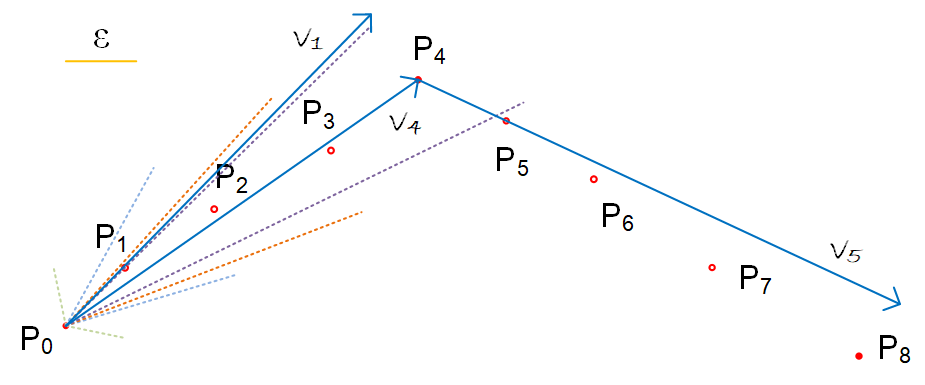
\includegraphics[scale=1.0]{figures/Fig-SITT.png}
	\vspace{-2ex}
	\caption{\small A running example of trajectory tracking by \sitt.  }
	\vspace{-2ex}
	\label{fig:sitt}
\end{figure}



\begin{example}
	Figure~\ref{fig:bitt} is a running example of \bitt. It takes as inputs the same trajectory as the above, the same $\epsilon_{sed}$ as Figure~\ref{fig:citt} and an $\epsilon_{ped}$ of half that of Figure~\ref{fig:sitt}. Because its $\epsilon_{sed}$ is the same as Figure~\ref{fig:citt}, its effectiveness is also the same as Figure~\ref{fig:citt}. For the purpose of clearness, we do not show those cones in the figure.
	%
	\bitt uses full-$\epsilon_{sed}$ cones and full-$\epsilon_{ped}$ sectors to simplify the trajectory. Initially, it sets the same start point and initial velocity as Figure~\ref{fig:citt}, 
	Then, (1) $P_3$ lives in the common intersection of the preview cones and sectors, and it has both \sed and \ped distances larger than $\epsilon_{sed}$ and $\epsilon_{ped}$, respectively, \ie $|P_3P'_3| \ge \epsilon_{sed}$ and $|P_3P^*_3| \ge \epsilon_{ped}$, thus, \bitt updates the velocity from $\vec{v_1}$ to $\vec{v_3}$ and the process goes on, (2) $P_5$ is outside of the common intersections of the preview cones and sectors, thus, $P_4$ serves as the new start point, and an update of $(P_4, \vec{v_5})$ is triggered, and (3) $P_7$ lives in the common intersections of the preview cones and sectors, and it has a \ped distance larger than $\epsilon_{ped}$, thus, \bitt updates the velocity from $\vec{v_5}$ to $\vec{v_7}$ (not shown) and the process goes on. Finally, it sends three points, $P_0, P_4$ and $P_8$, and four velocities, $\vec{v_1}$, $\vec{v_3}$, $\vec{v_5}$ and $\vec{v_7}$, to the MOD server. 
\end{example}

\begin{figure}[tb!]
	\centering
	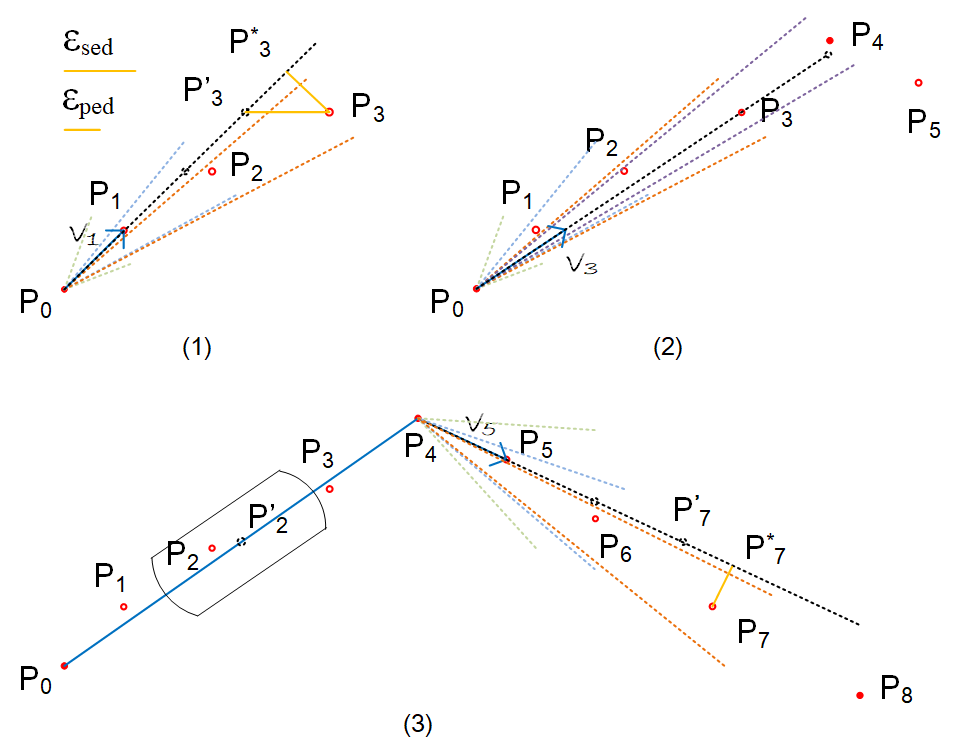
\includegraphics[scale=1.0]{figures/Fig-BITT.png}
	\vspace{-2ex}
	\caption{\small A running example of trajectory tracking by \bitt. In this case, the spatio-temporal cones and their intersections are the same as Figure~\ref{fig:citt}, thus they are not shown here for clearness.  }
	\vspace{-2ex}
	\label{fig:bitt}
\end{figure}





\stitle{Correctness and complexity.} 
\myblue{The correctness of algorithm \bitt follows from Theorems \ref{theo-full-cone}, \ref{theo-full-sector} and \ref{theo-binary}.
It is also easy to find that it has a linear time complexity like \citt and \sitt.}


%\stitle{Discuss.} Relations to position tracking and traj simplification. 

%\input{sec-track-in-rectangle-like}
%%% Local Variables:
%%% mode: latex
%%% TeX-master: "gis18"
%%% End:
\section{Experimental Study}
\label{sec-exp}

\eat{
\begin{table*}[!ht]
	\renewcommand{\arraystretch}{1.20}
	\caption{\small Real-life Trajectory Datasets}
	\vspace{-1.5ex}
	\centering
	\footnotesize
	%\scriptsize
	\begin{tabular}{|l|c|c|c|r|}
		\hline
		\bf{ Data Sets}& \bf{Number\ of Trajectories}     &\bf {Sampling Rates\ (s)}   &\bf{Points Per Trajectory\ (K)}    &\bf {Total points} \\
		\hline
		\sercar	&1,000	    &3-5	    &$\sim114.0$   &114M\\
		\hline
		\geolife &182	    &1-5	    &$\sim131.4$   &24.2M\\
		\hline
		\mopsi &51	    	&2	    &$\sim153.9$     &7.9M\\
		\hline
	\end{tabular}
	\label{tab:datasets}
	\vspace{-2ex}
\end{table*}
}

\begin{table}[!ht]
	\renewcommand{\arraystretch}{1.20}
	\caption{\small Real-life Trajectory Datasets}
	\vspace{-1.5ex}
	\centering
	\footnotesize
	%\scriptsize
	\begin{tabular}{|l|c|c|r|}
		\hline
		\bf{ Properties of Data Sets} & \sercar      &\geolife   &\mopsi \\
		\hline
		{Number\ of Trajectories}	&1,000	    &182	    & 51  \\
		\hline
		 {Sampling Rates\ (s)} &3-5  & 1-5 & 2 \\
		\hline
		{Points Per Trajectory\ (K)}  &	$\sim114.0$    &$\sim131.4$	    & $\sim153.9$ \\
		\hline
		 {Total points (M)} &114   	    	&24.2    &7.9\\
		\hline
	\end{tabular}
	\label{tab:datasets}
	\vspace{-2ex}
\end{table}


In this section, we present an extensive experimental study of our one-pass trajectory tracking algorithms (\citt, \sitt and \bitt) compared with the
existing algorithms of \ldrh and \grts on trajectory datasets. Using three real-life trajectory datasets, we conducted sets of experiments to evaluate:
(1) the number of messages (including data points and velocities),
(2) the compression ratios,
(3) the average errors, and
(4) the running time of algorithms \citt, \sitt and \bitt vs. \ldrh and \grts. 
Among them, the impacts of error bounds and distance metrics on messages, errors and running time of these algorithms are evaluated. 

\subsection{Experimental setting}

\stitle{Real-life Trajectory Datasets}. We use three reallife datasets ServiceCar, GeoLife and Mopsi shown in Table \ref{tab:datasets} to test our solutions.

\vspace{0.5ex}
\ni \emph{(1) Service car trajectory data} (\sercar) is the GPS trajectories collected by a Chinese car rental company during Apr. 2015 to Nov. 2015. The sampling rate was one point per $3$--$5$ seconds, and
each trajectory has around $114.1K$ points.

\vspace{0.5ex}
\ni \emph{(2) GeoLife trajectory data} (\geolife) is the GPS trajectories collected in GeoLife project by 182 users in a period from Apr. 2007 to Oct. 2011. These trajectories have a variety of sampling rates, among which 91\% are logged in each 1-5 seconds per point. %or each 5-10 meters

\vspace{0.5ex}
\ni \emph{(3) Mopsi trajectory data} (\mopsi) is the GPS trajectories collected in Mopsi project by 51 users in a period from 2008 to 2014. Most routes are in Joensuu region, Finland.
The sampling rate was one point per $2$ seconds, and each trajectory has around $153.9K$ points.

\stitle{Metrics.}
Following the main stream \cite{Trajcevski:LDRH, Lange:GRTS, Lange:Tracking, Lin:Cised, Zhang:Evaluation}, we use \emph{messages}, \emph{compression ratio}, \emph{average error} and \emph{running time} to evaluate algorithms.

 \ni \emph{(1) Total messages}. It is the ratio of the total number of messages (velocities and data points) \wrt the total number of the original trajectory points
 
 \ni \emph{(2) Compression ratio}. It is defined as follows: Given a set of trajectories $\{\dddot{\mathcal{T}_1}, \ldots, \dddot{\mathcal{T}_M}\}$ and their piecewise line representations $\{\overline{\mathcal{T}_1}, \ldots, \overline{\mathcal{T}_M}\}$, the compression ratio of an algorithm is $(\sum_{j=1}^{M} |\overline{\mathcal{T}}_j |)/(\sum_{j=1}^{M} |\dddot{\mathcal{T}}_j |)$.
 By the definition, \emph{algorithms with lower compression ratios are better}.
 
 \ni \emph{(3) Average error}. It is the average value of the distances from every point of the original trajectories to its representing line segment of the simplified trajectories.
 
 \ni \emph{(4) Running time}. It is the efficiency of the algorithms.
 
\stitle{Algorithms and implementation}.
We implement five tracking algorithms, \ie our \citt, \sitt and \bitt, \ldrh (the first and the most efficient) and \grts (the most effective).
All algorithms were implemented with Java.
All tests were run on an {x64-based  PC with 8 Intel(R) Core(TM) i5-6500 CPU @ 3.20GHz and 8GB of memory.
%, and each test was repeated over 3 times and the average is reported here.


\subsection{Experimental Results}


\begin{figure*}[tb!]
	\centering
	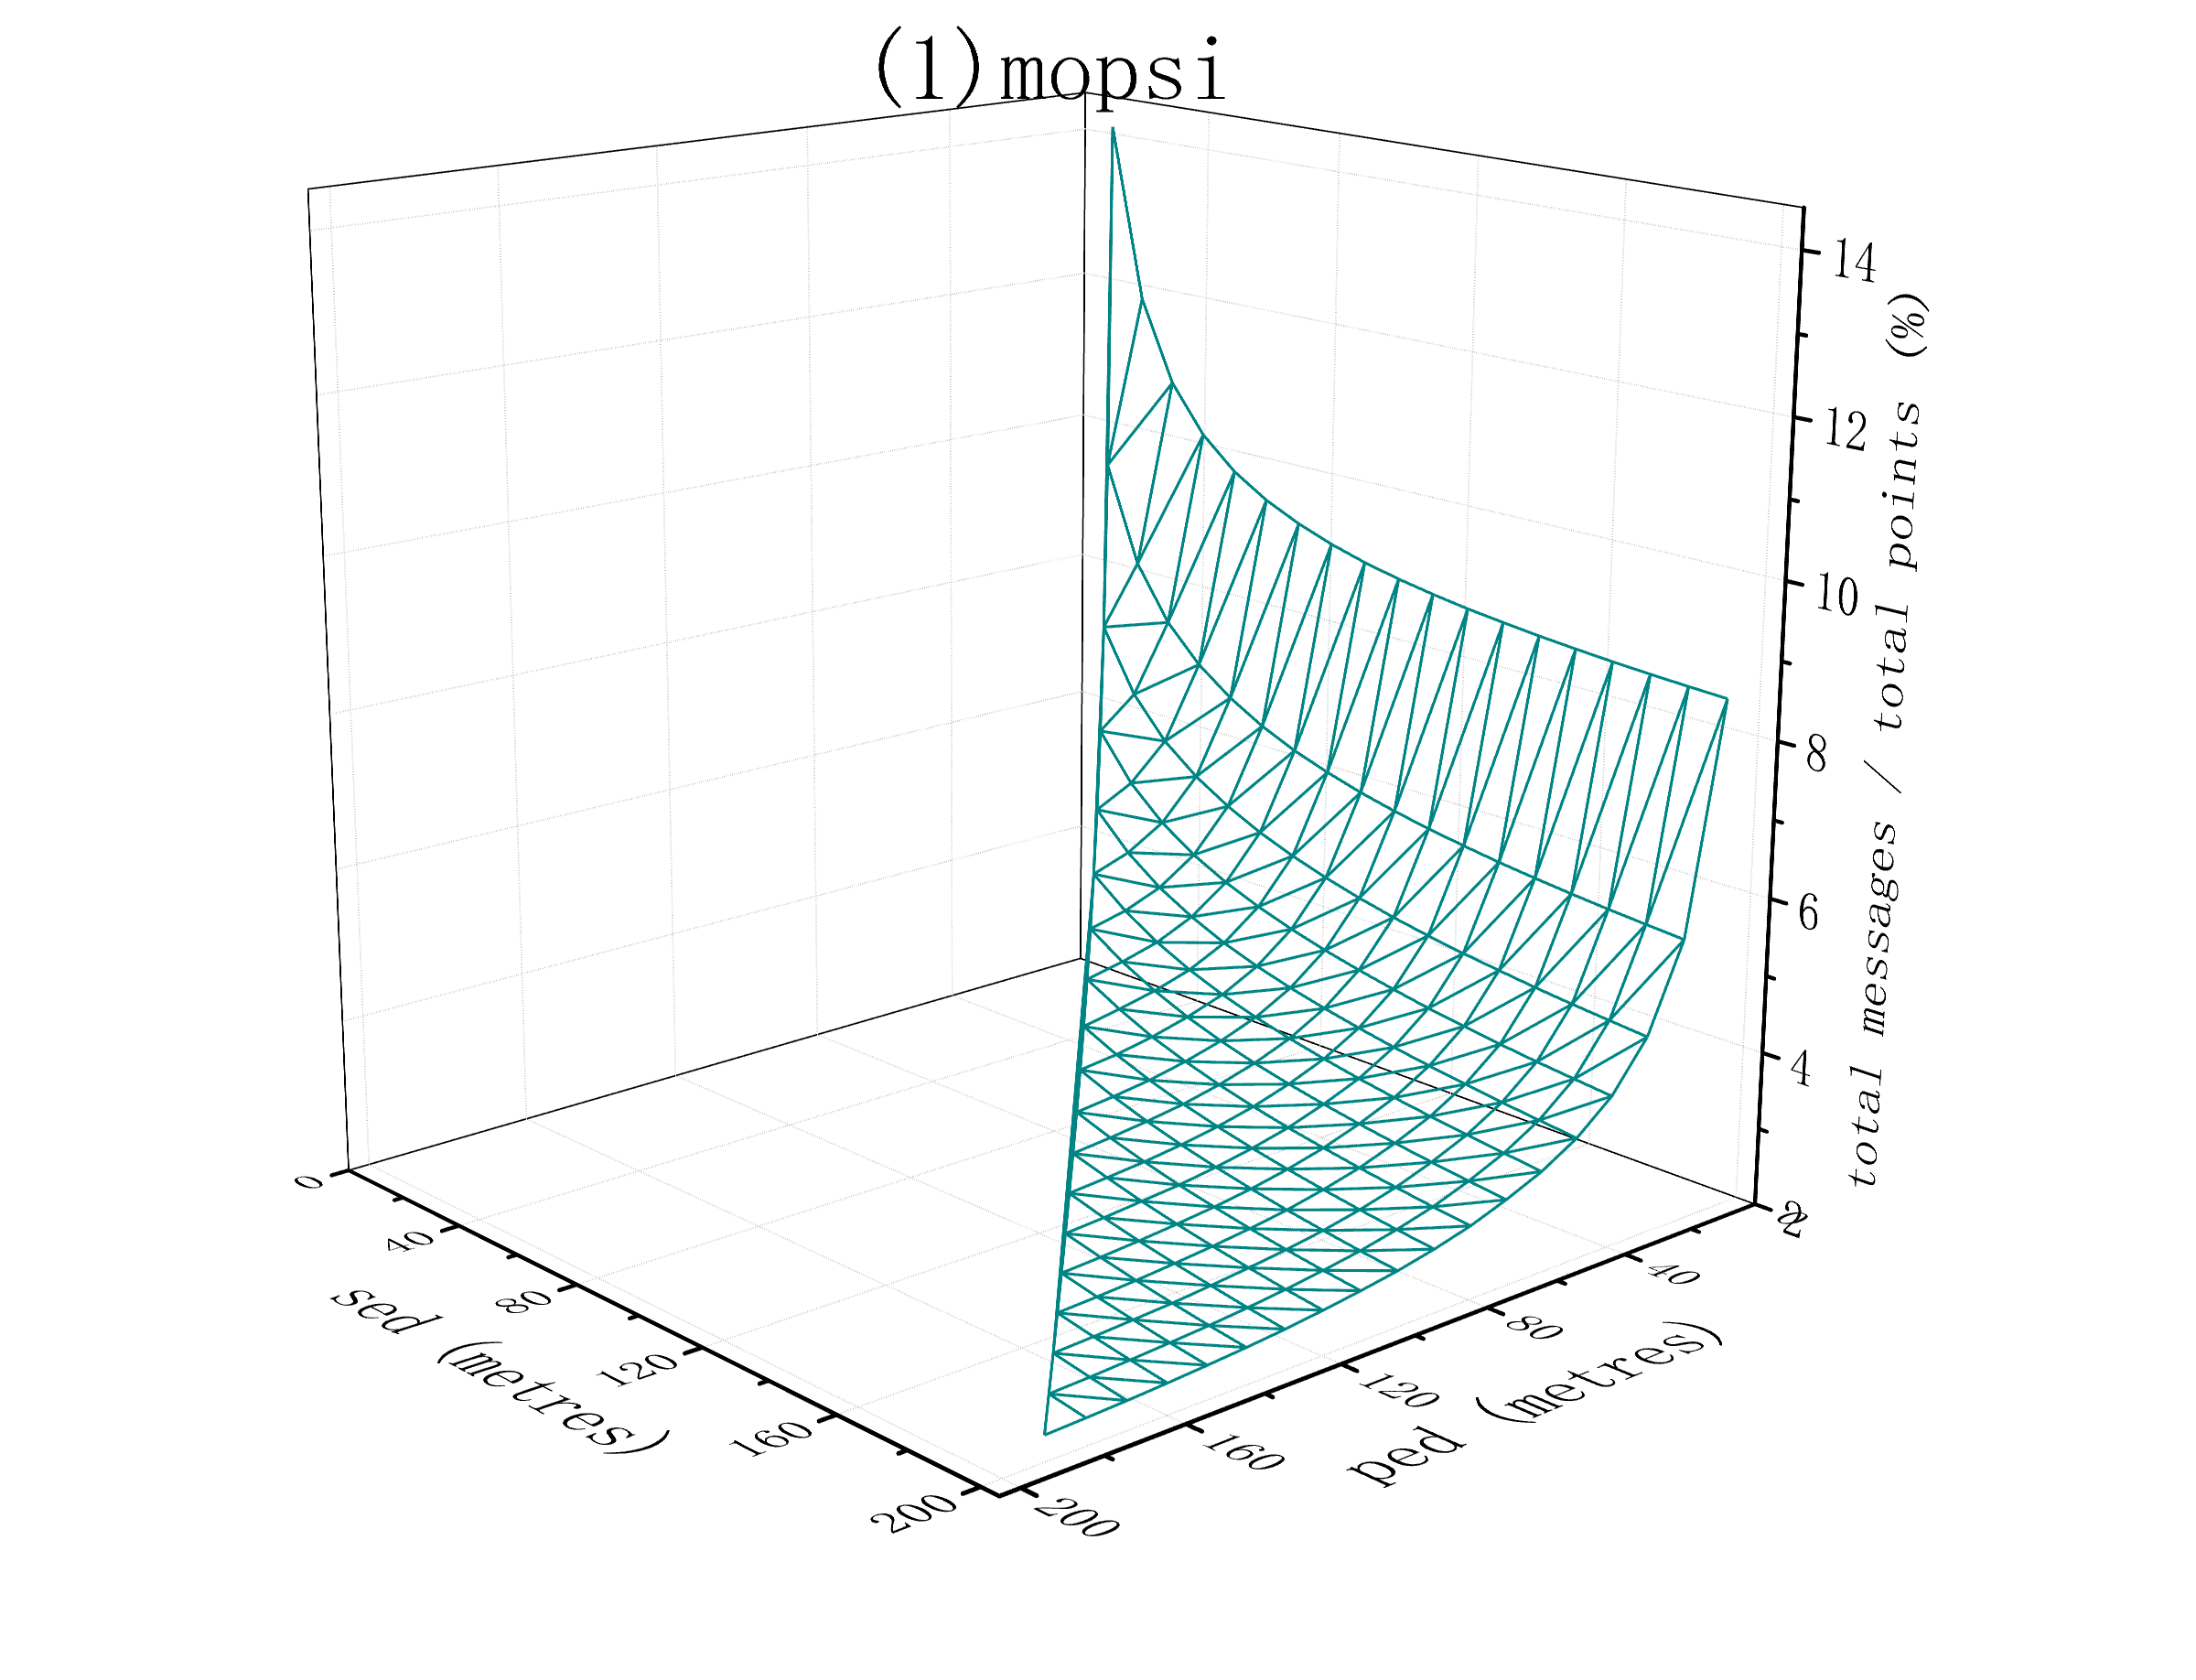
\includegraphics[scale = 0.210]{figures/Fig-BITT-mopsi-total-messages.png}\hspace{1ex}
	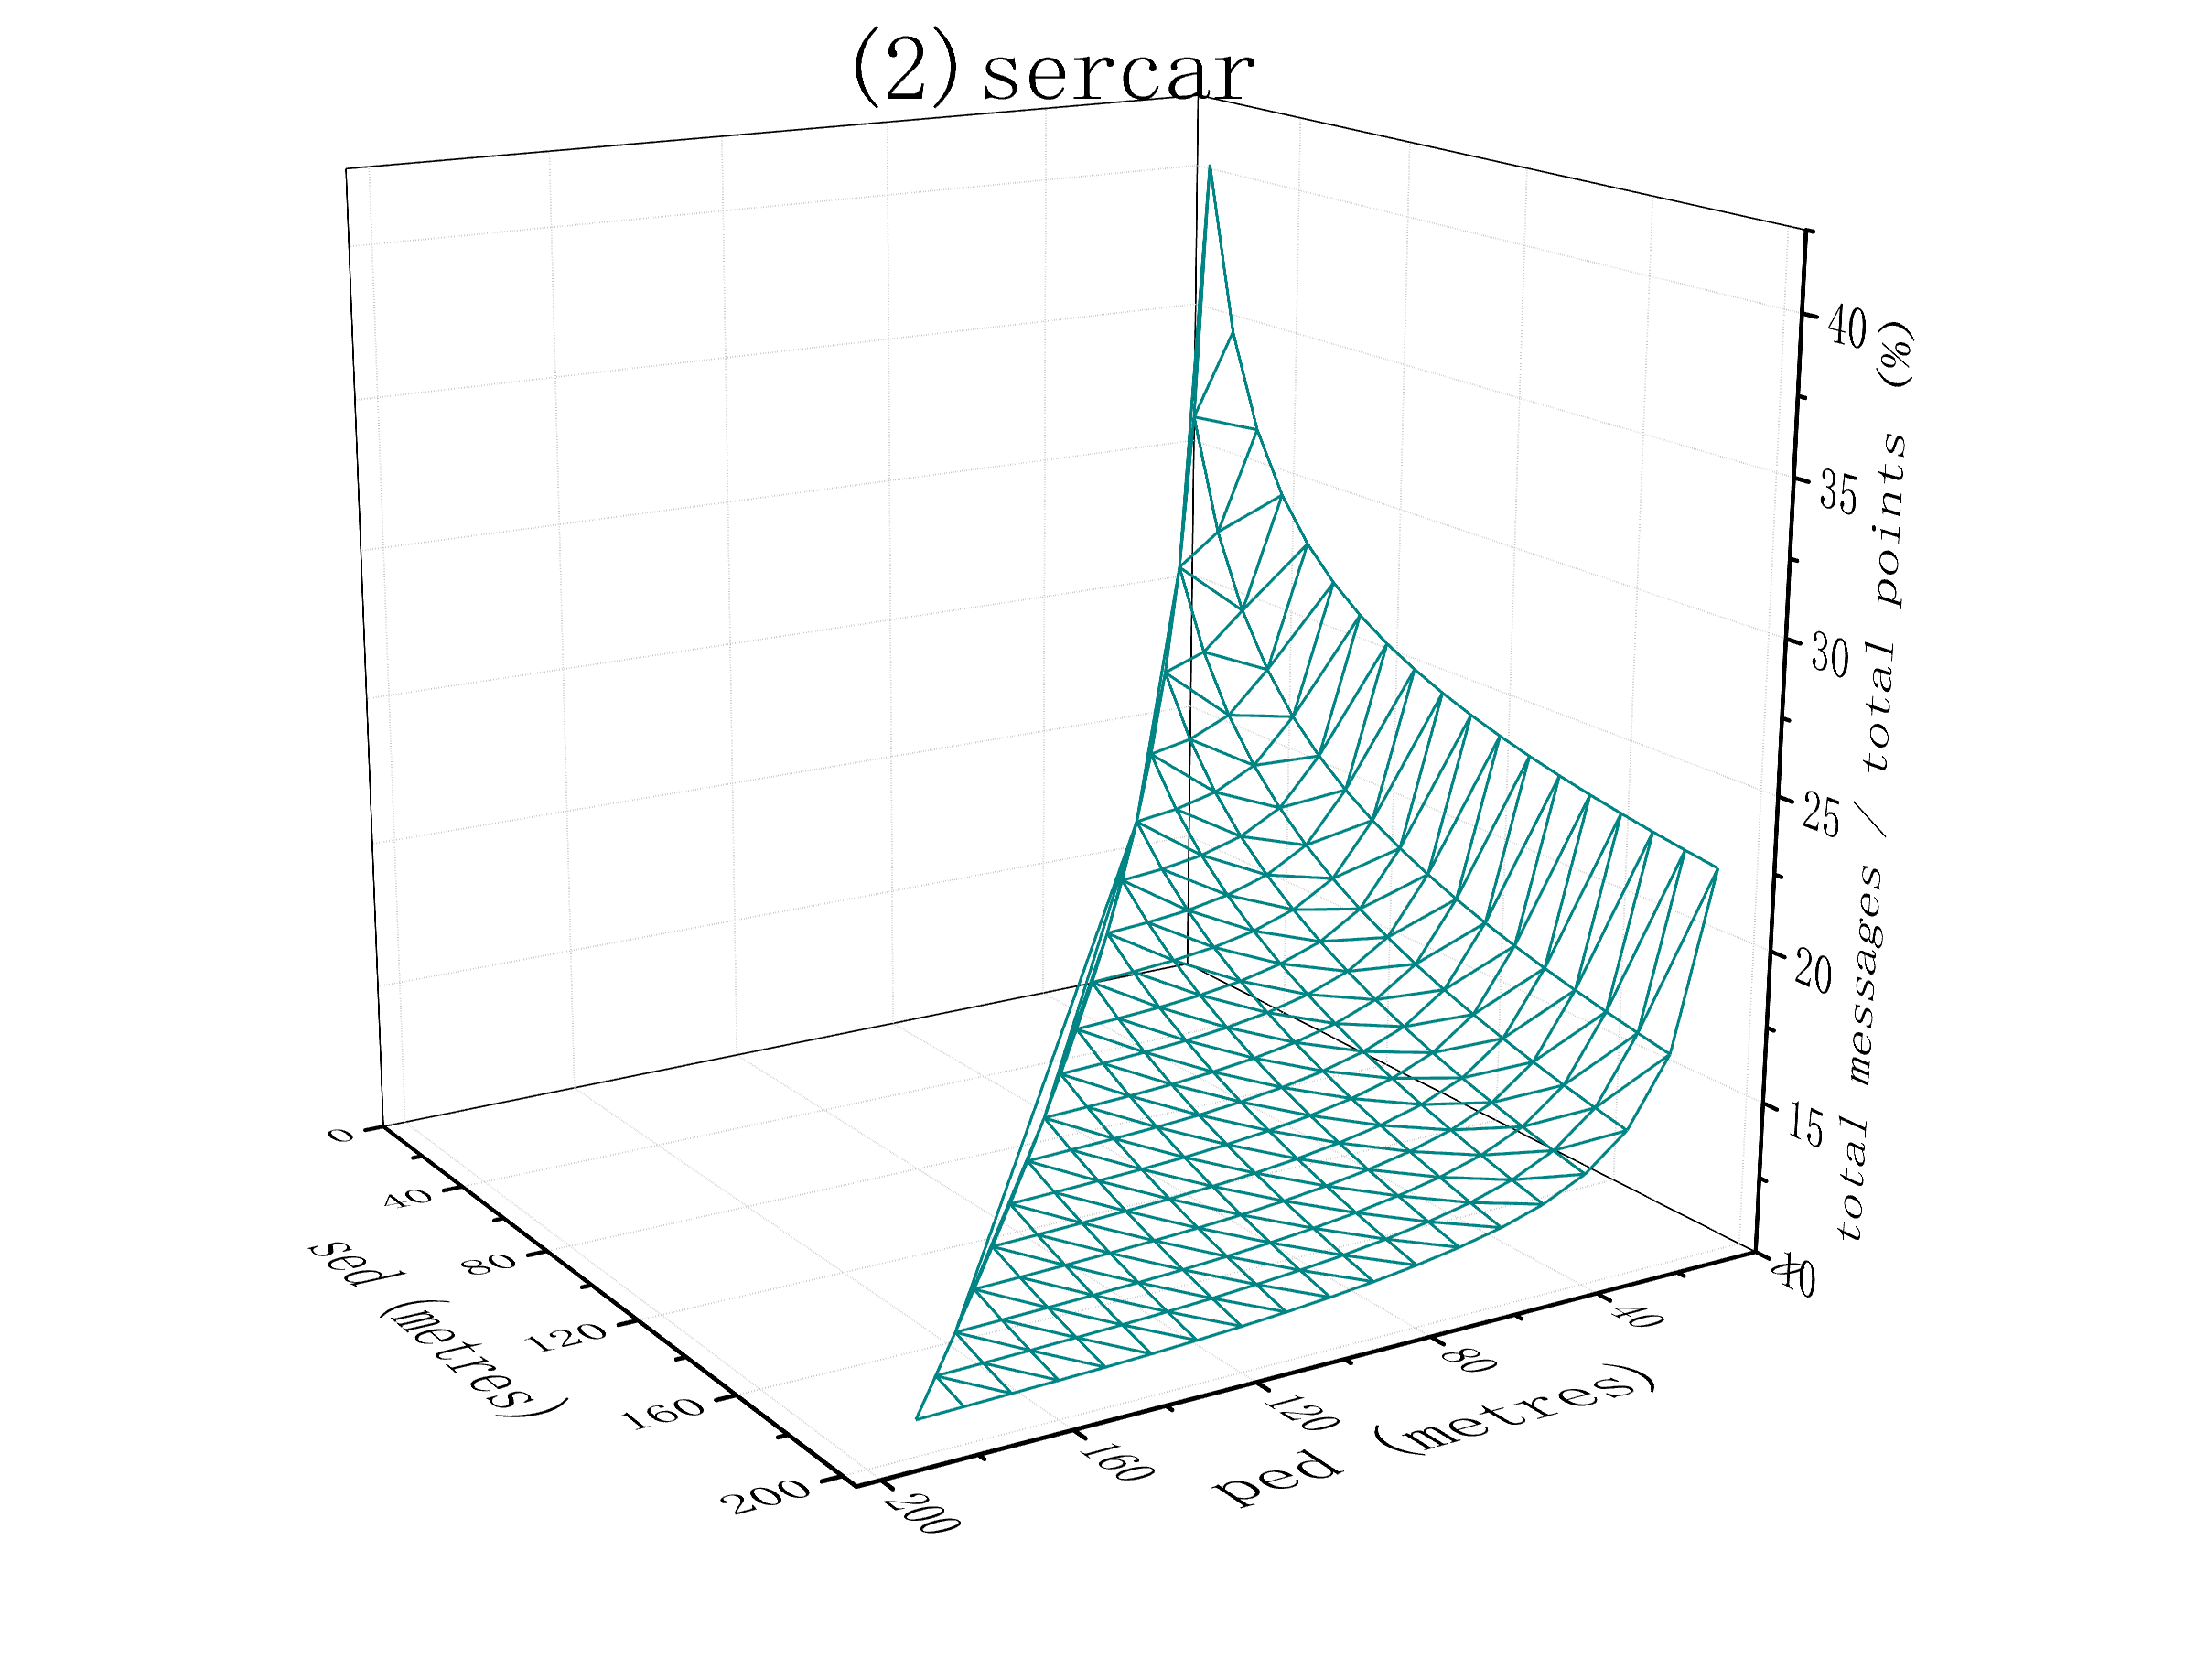
\includegraphics[scale = 0.210]{figures/Fig-BITT-sercar-total-messages.png}\hspace{1ex}
	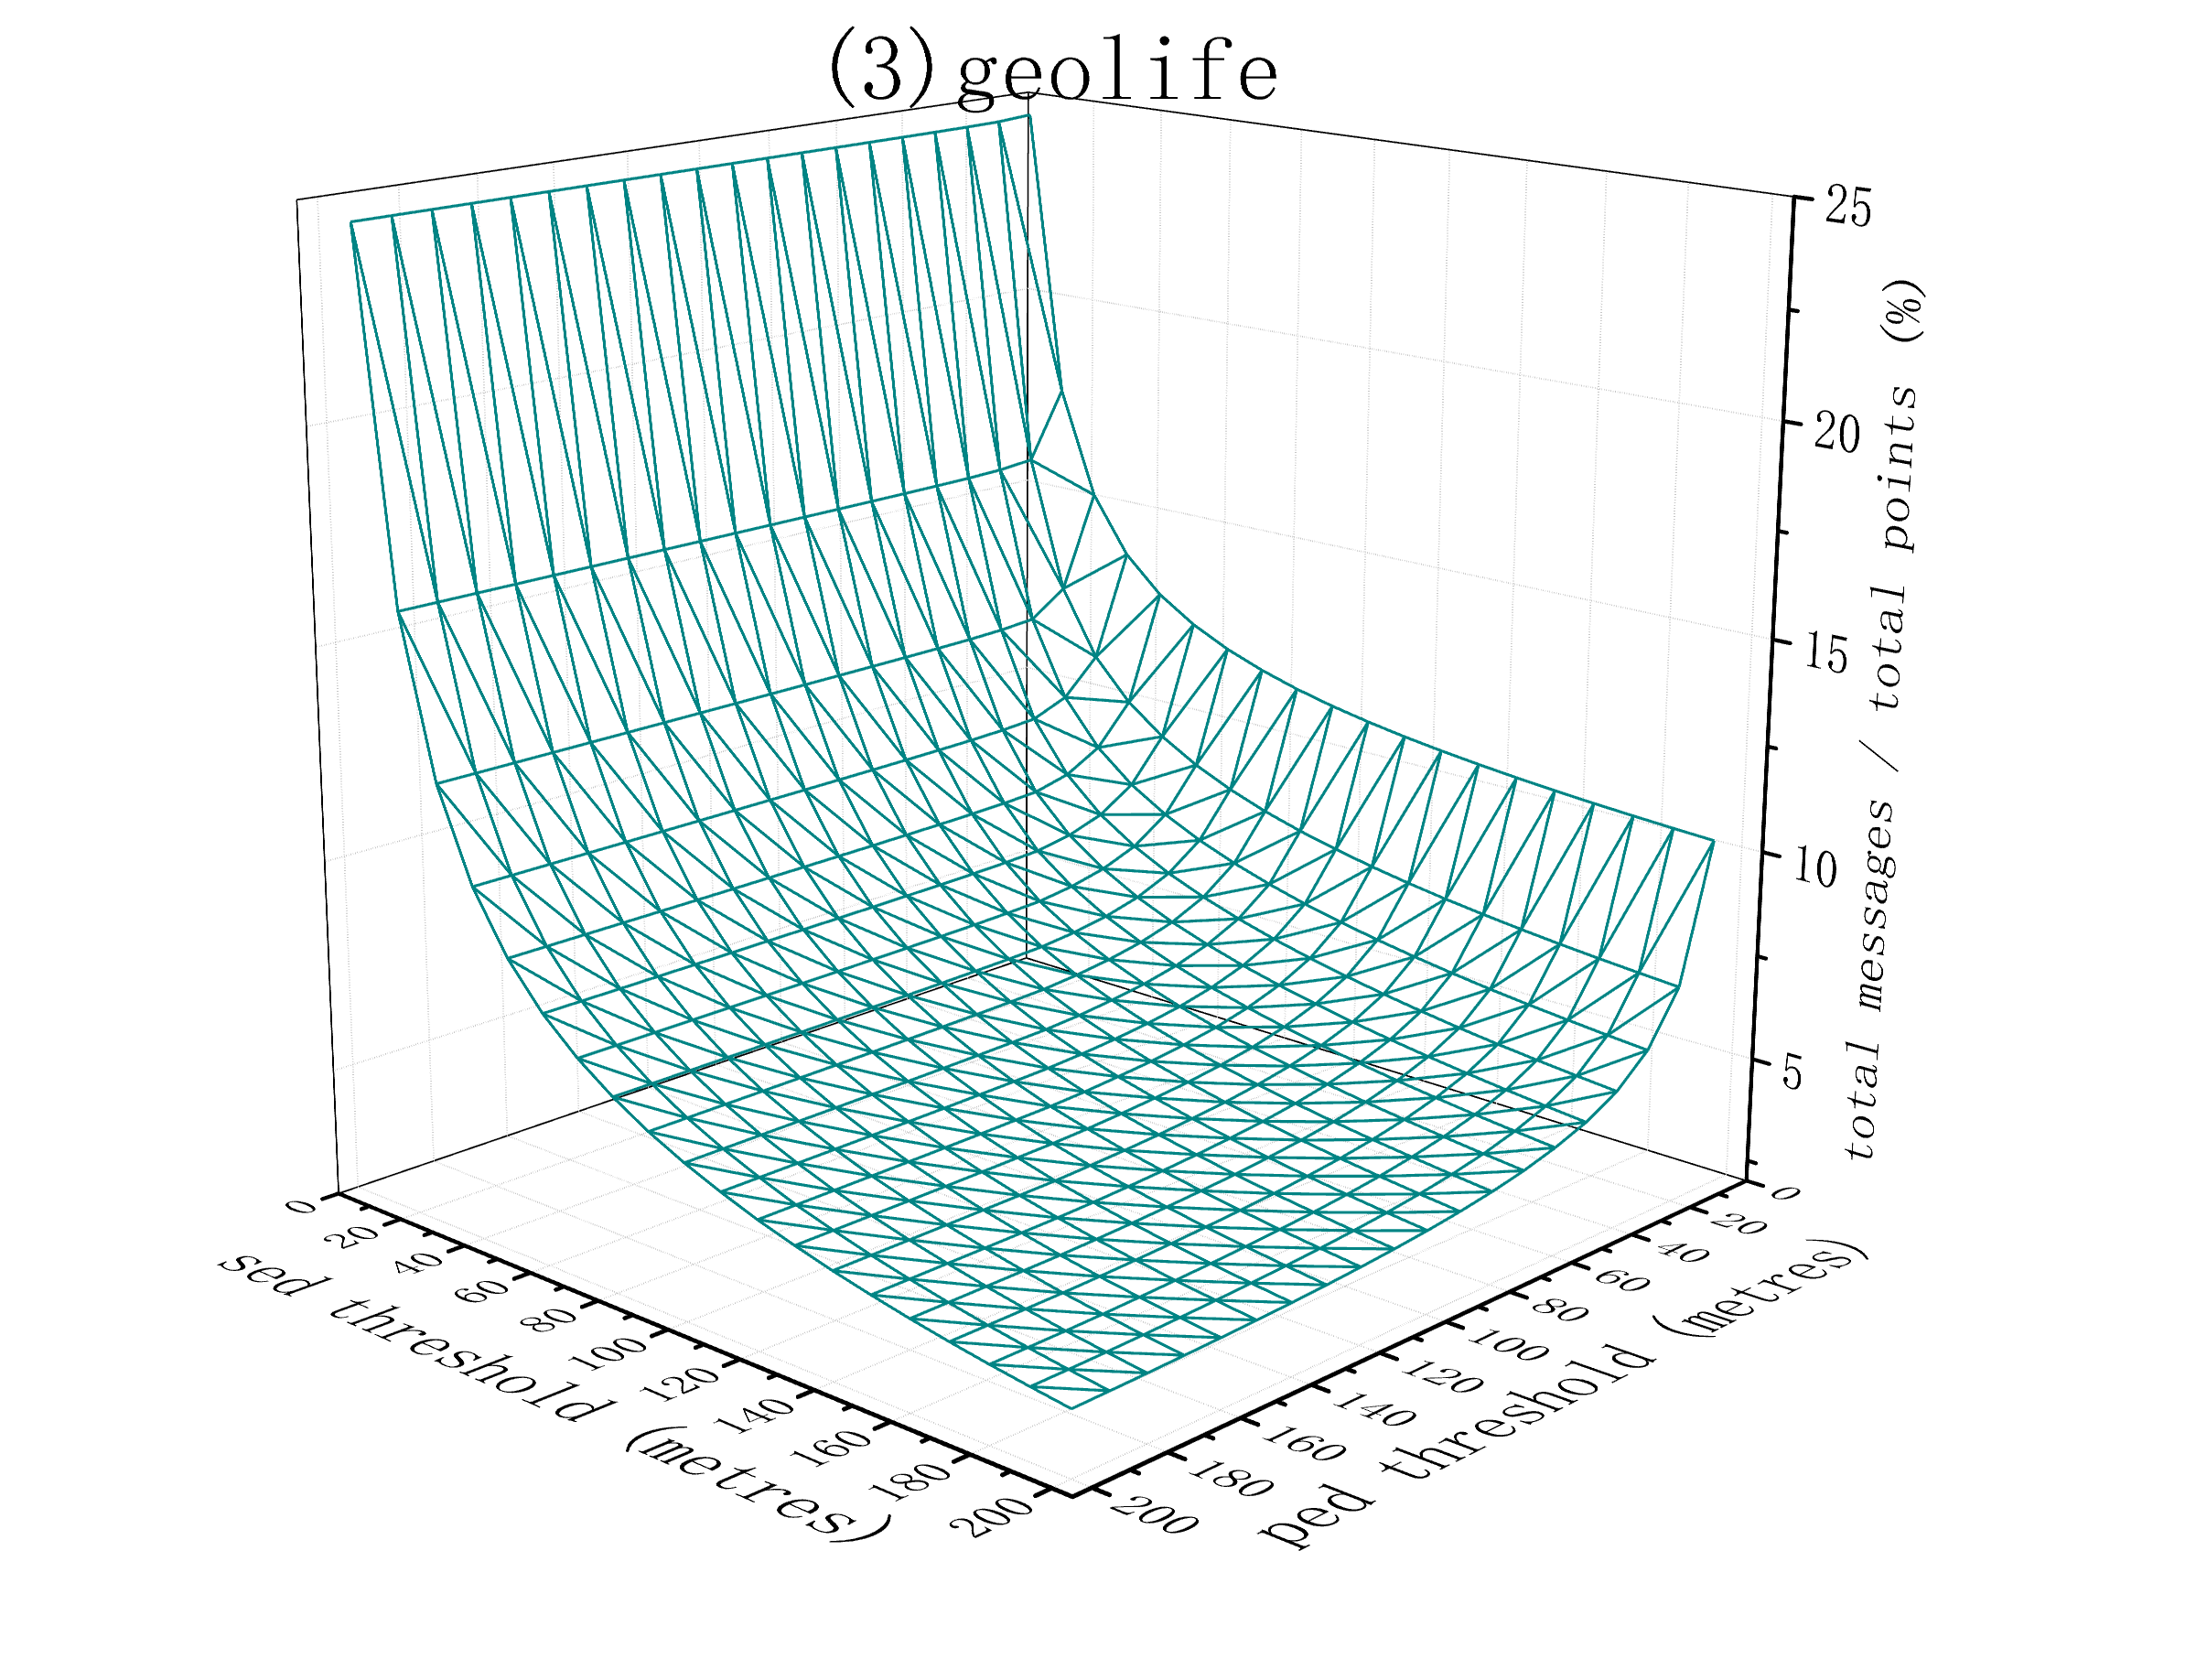
\includegraphics[scale = 0.210]{figures/Fig-BITT-geolife-total-messages.png}\hspace{1ex}
	\vspace{-2ex}
	\caption{\small Evaluation of BITT total messages: varying error bounds $\epsilon_{sed}$ and $\epsilon_{ped}$.}
	\label{fig:bitt-total-message}
	\vspace{-1ex}
\end{figure*}




\begin{figure*}[tb!]
	\centering
	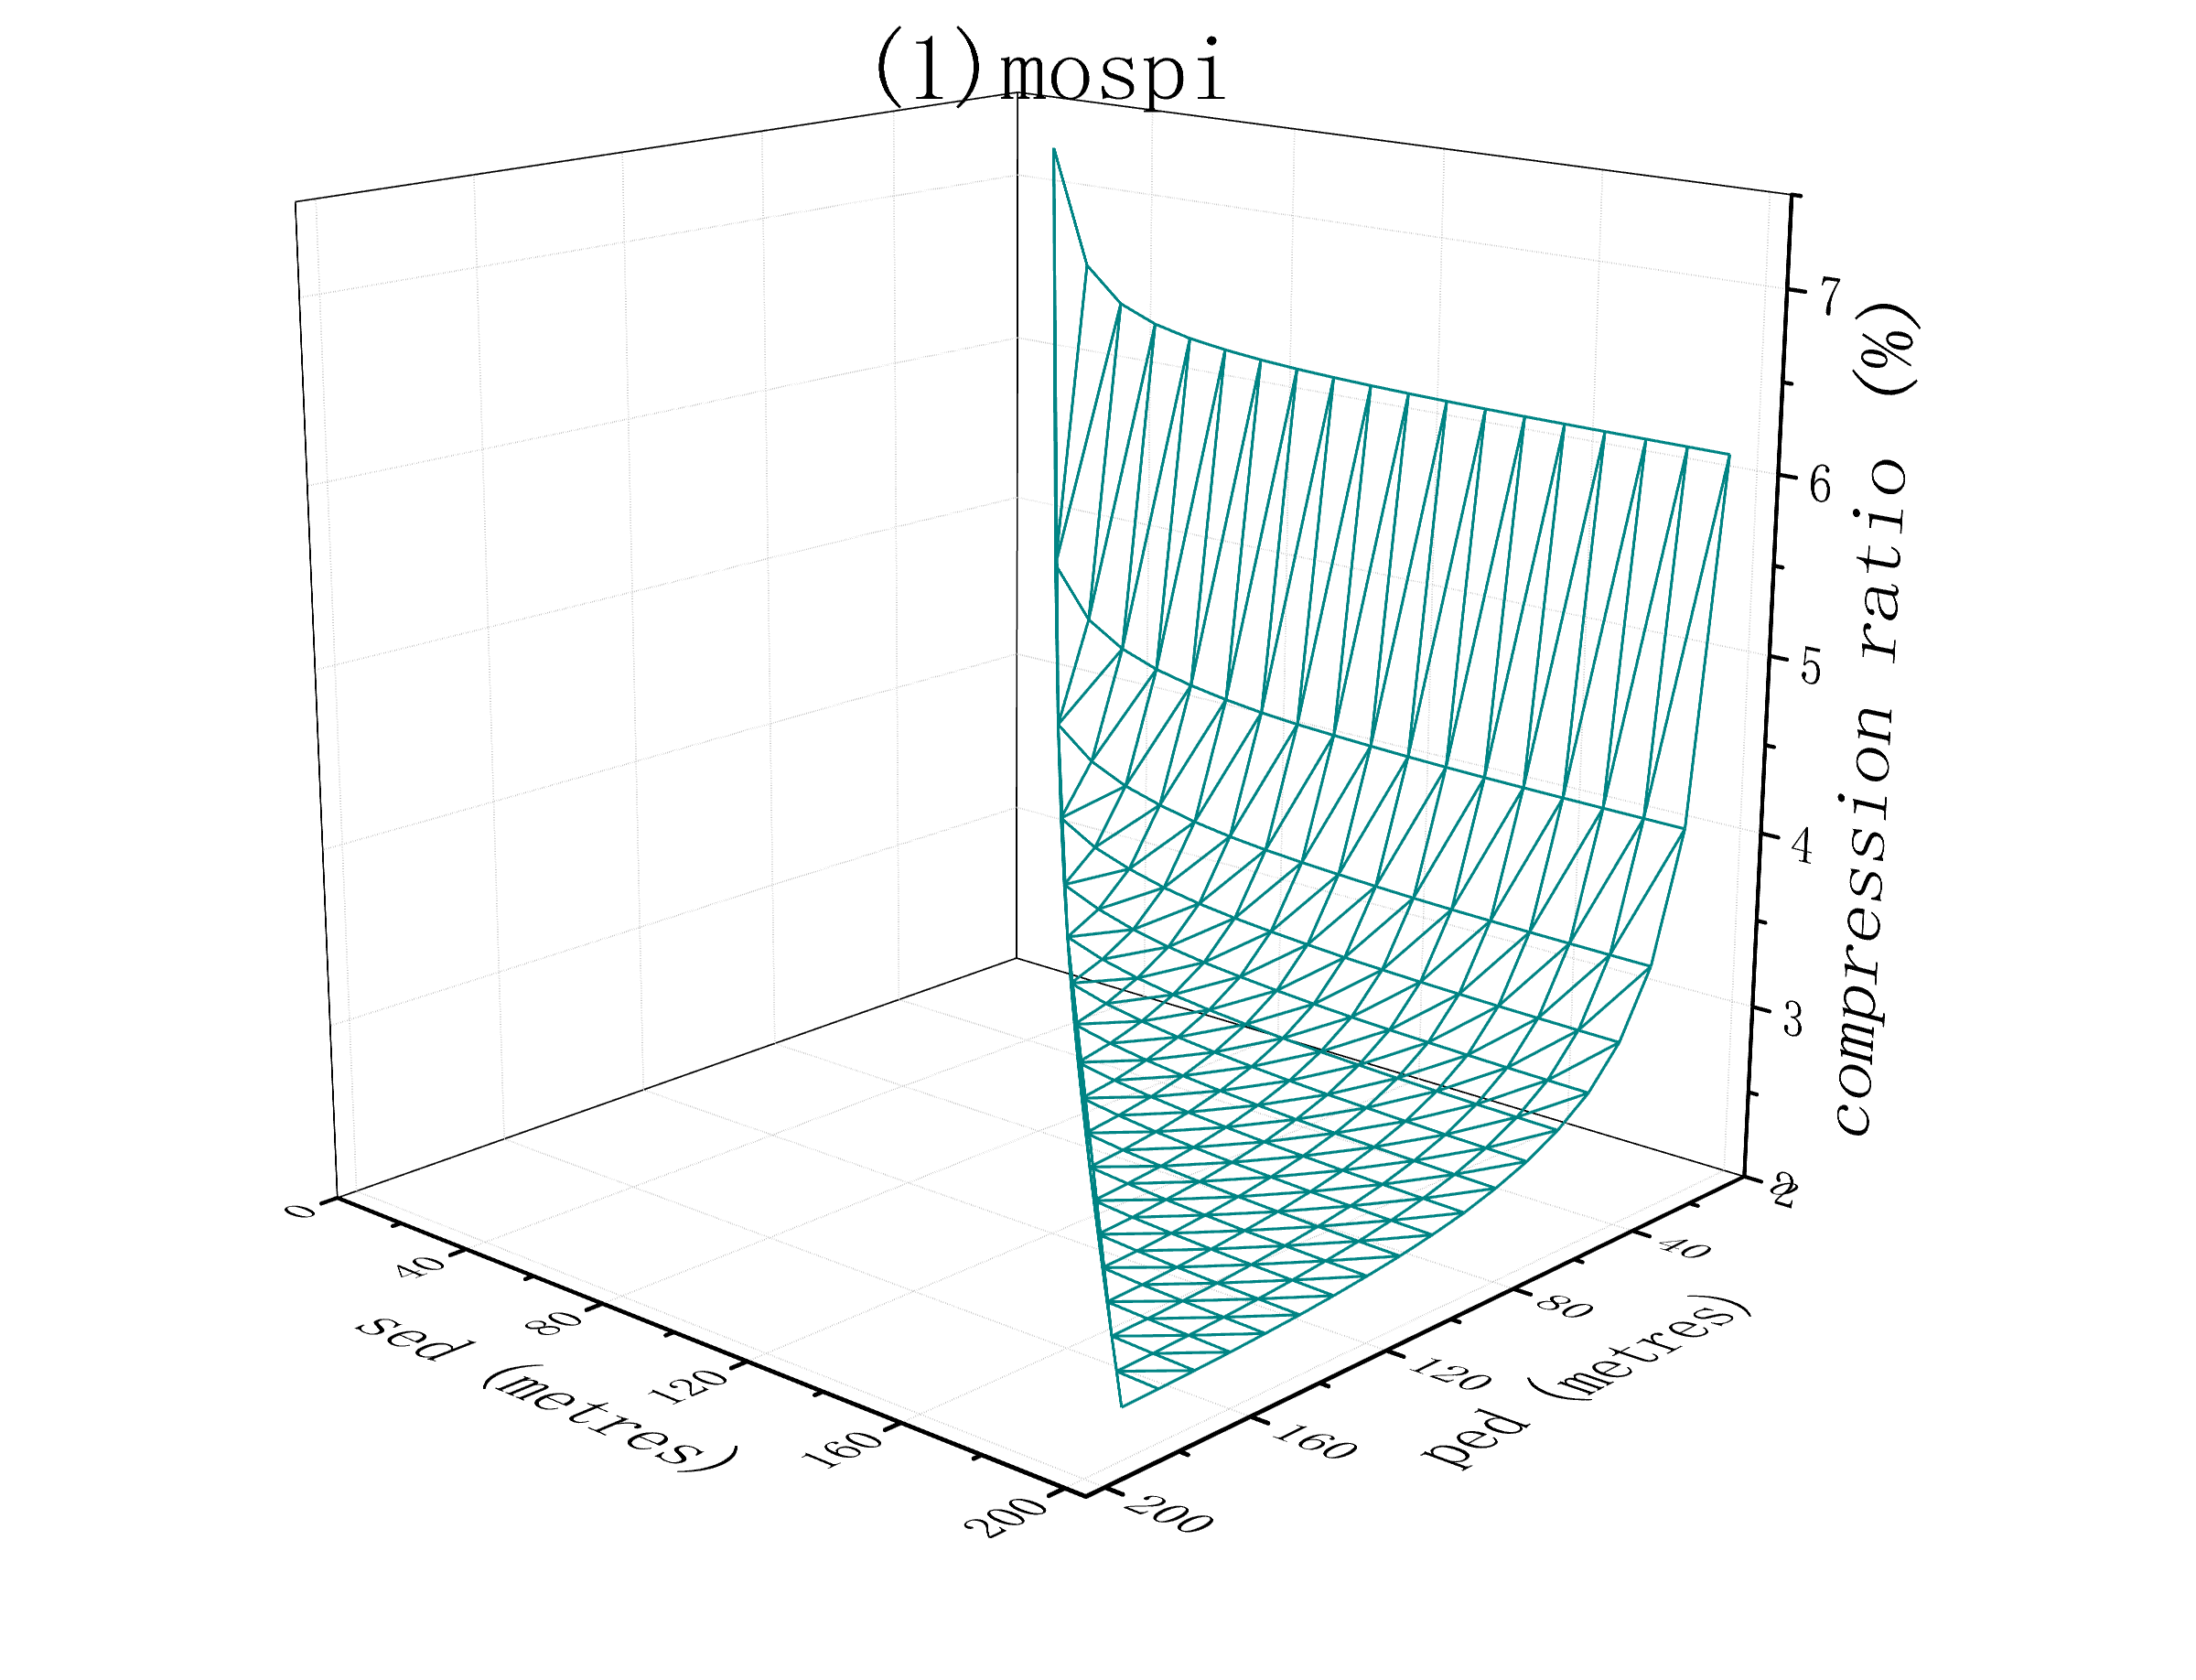
\includegraphics[scale = 0.210]{figures/Fig-BITT-mopsi-compression-ratio.png}\hspace{1ex}
	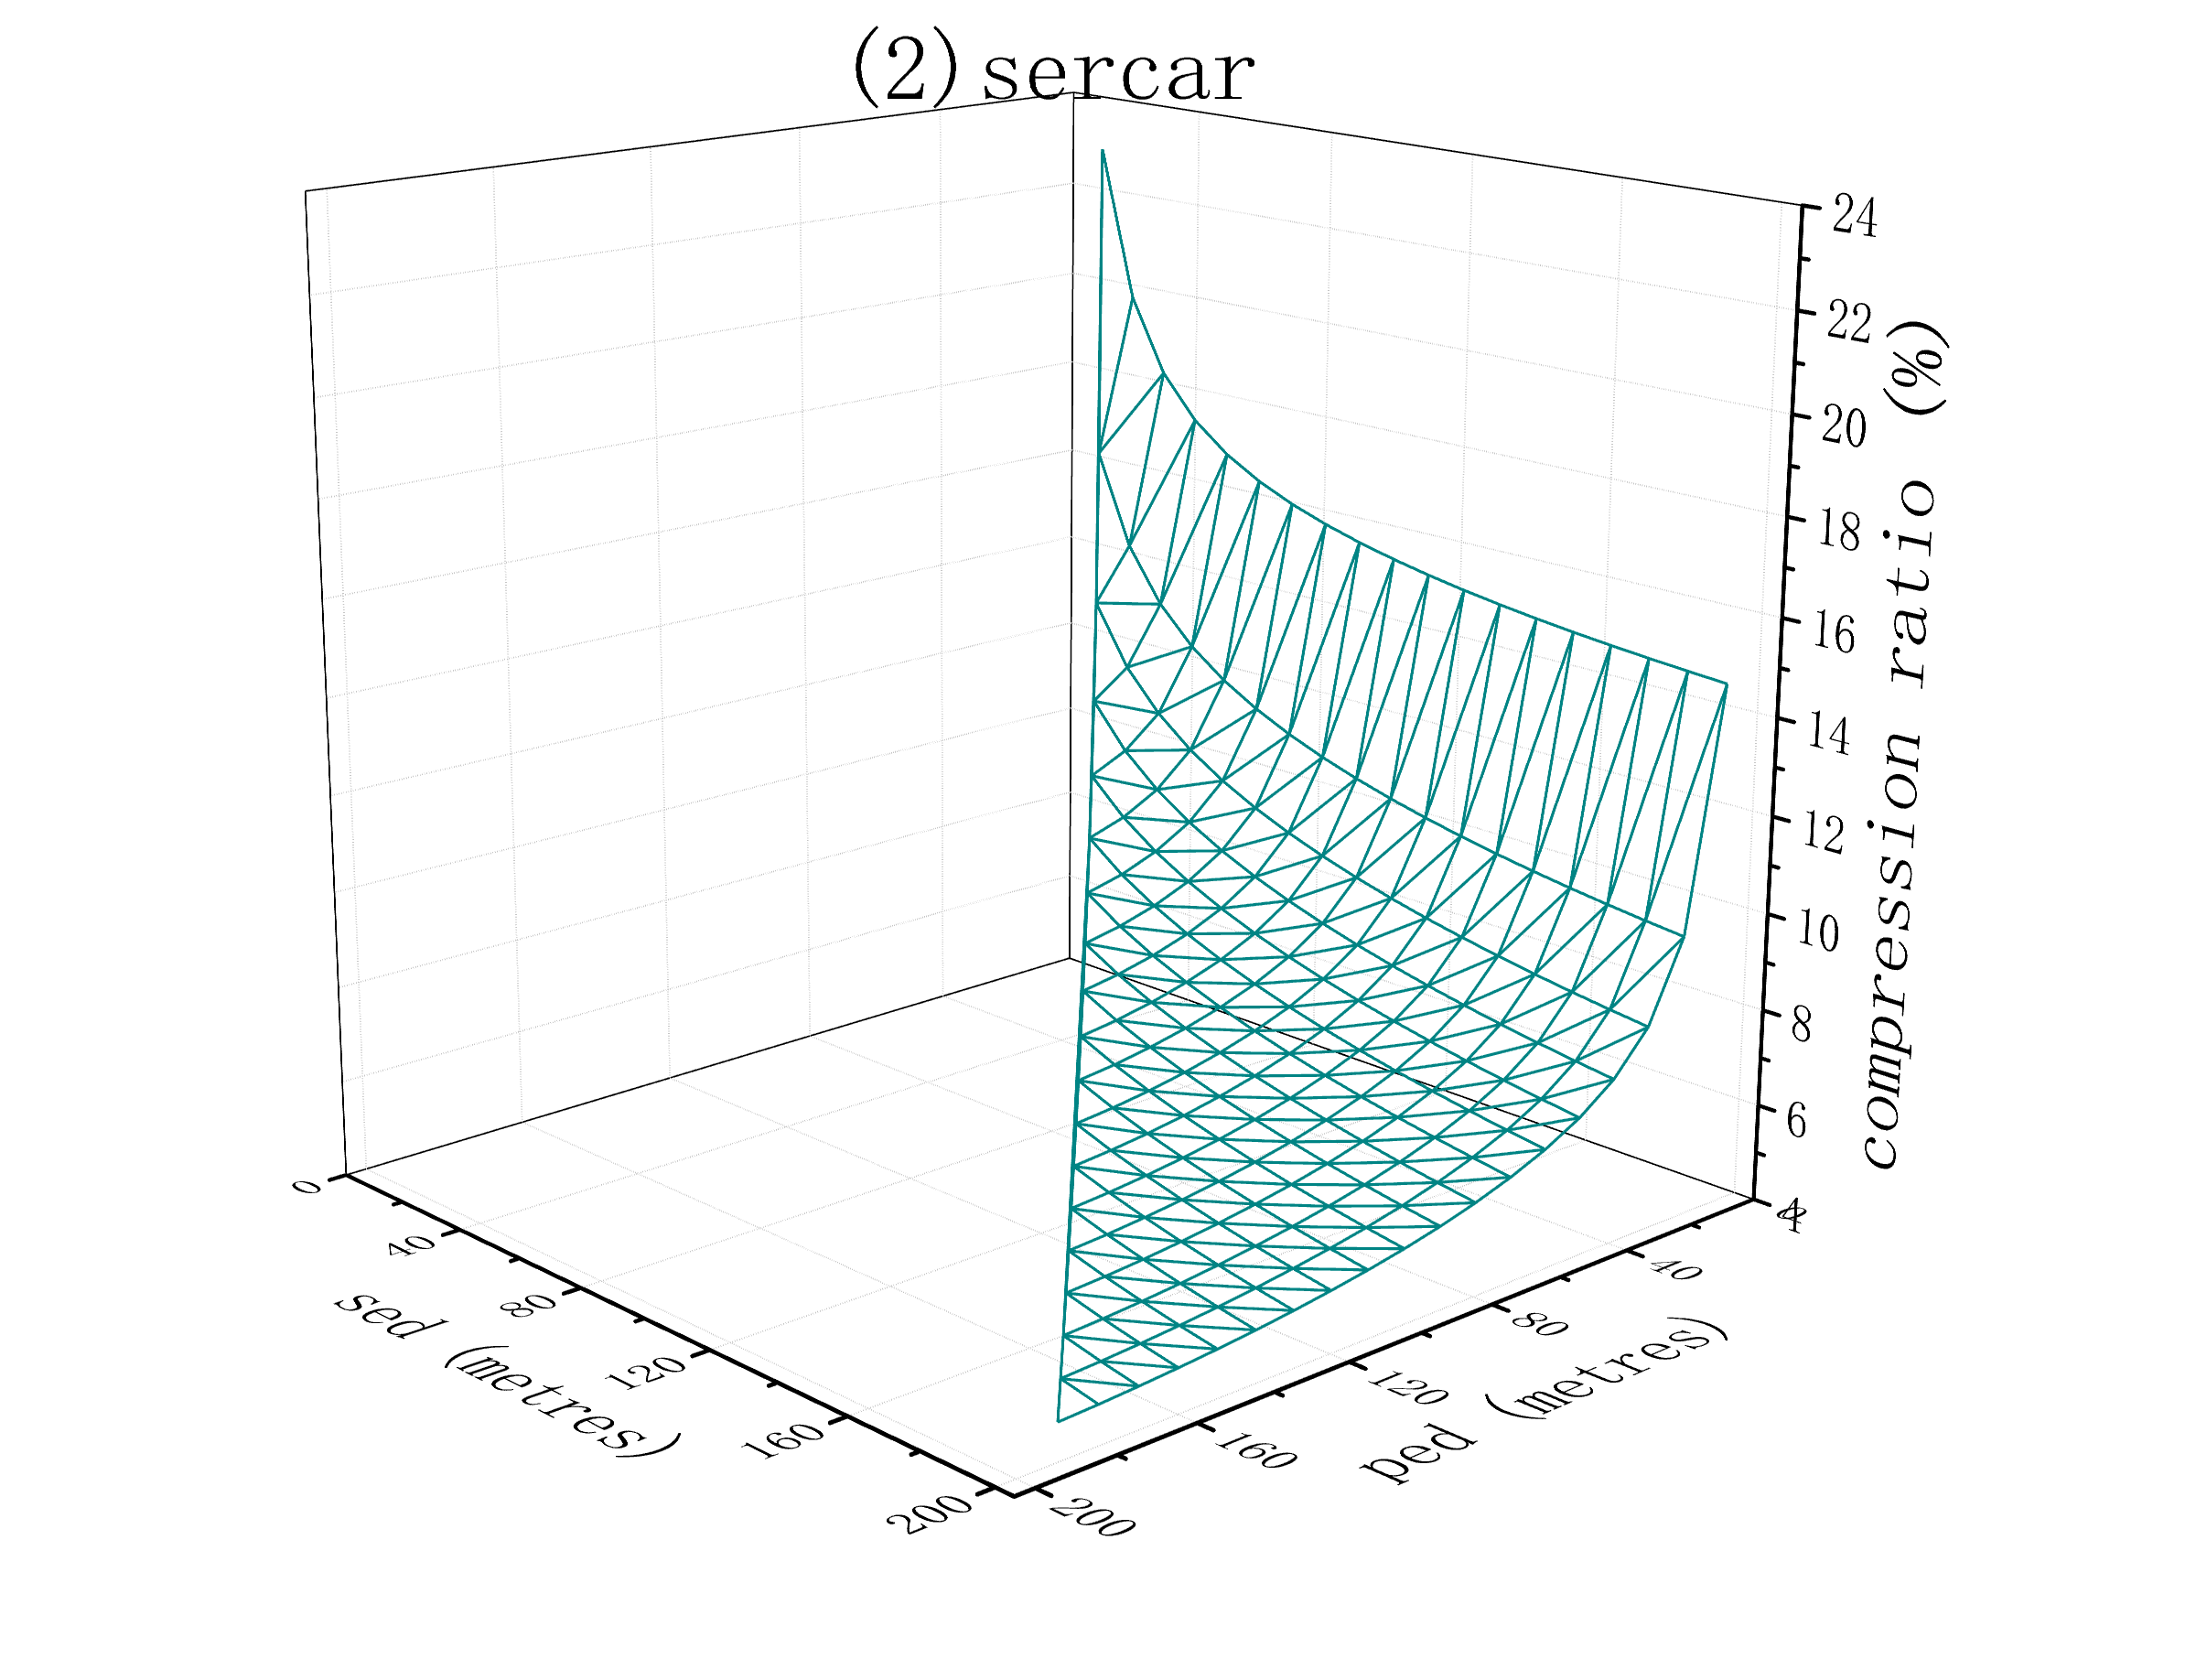
\includegraphics[scale = 0.210]{figures/Fig-BITT-sercar-compression-ratio.png}\hspace{1ex}
	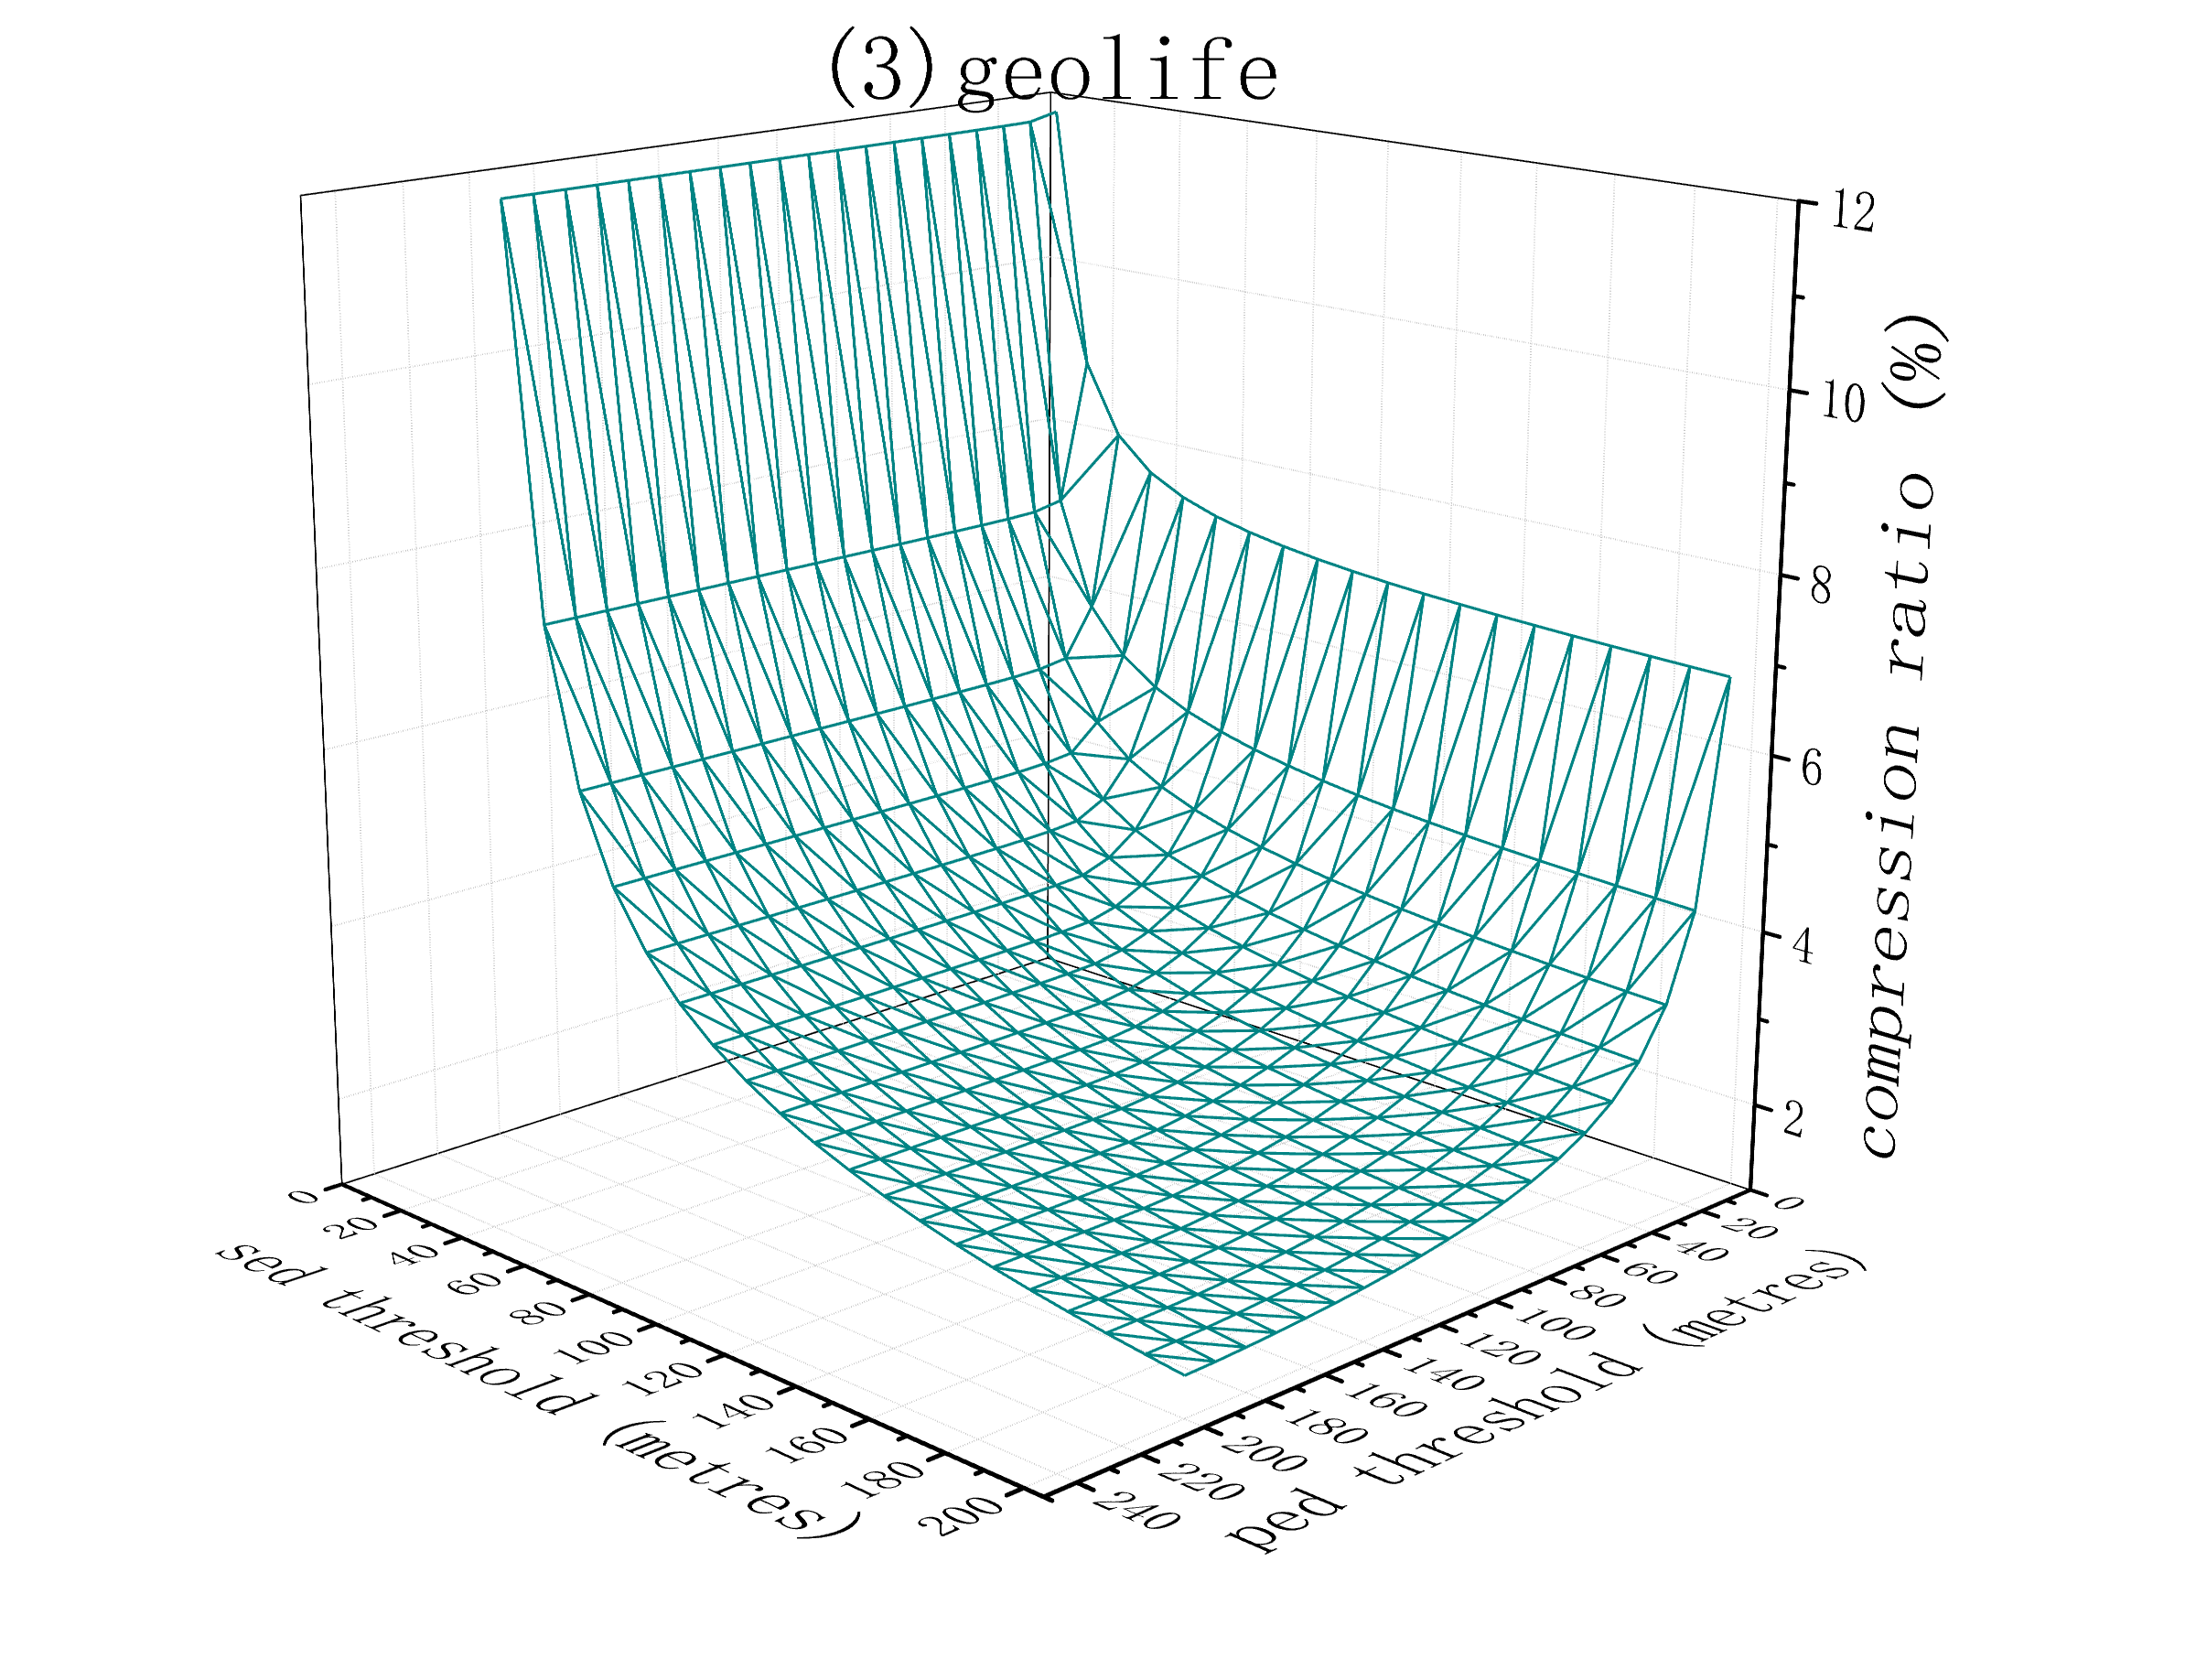
\includegraphics[scale = 0.210]{figures/Fig-BITT-geolife-compression-ratio.png}\hspace{1ex}
	\vspace{-2ex}
	\caption{\small Evaluation of BITT compression ratio: varying error bounds $\epsilon_{sed}$ and $\epsilon_{ped}$.}
	\label{fig:bitt-compression-ratio}
	\vspace{-1ex}
\end{figure*}


\begin{figure*}[tb!]
	\centering
	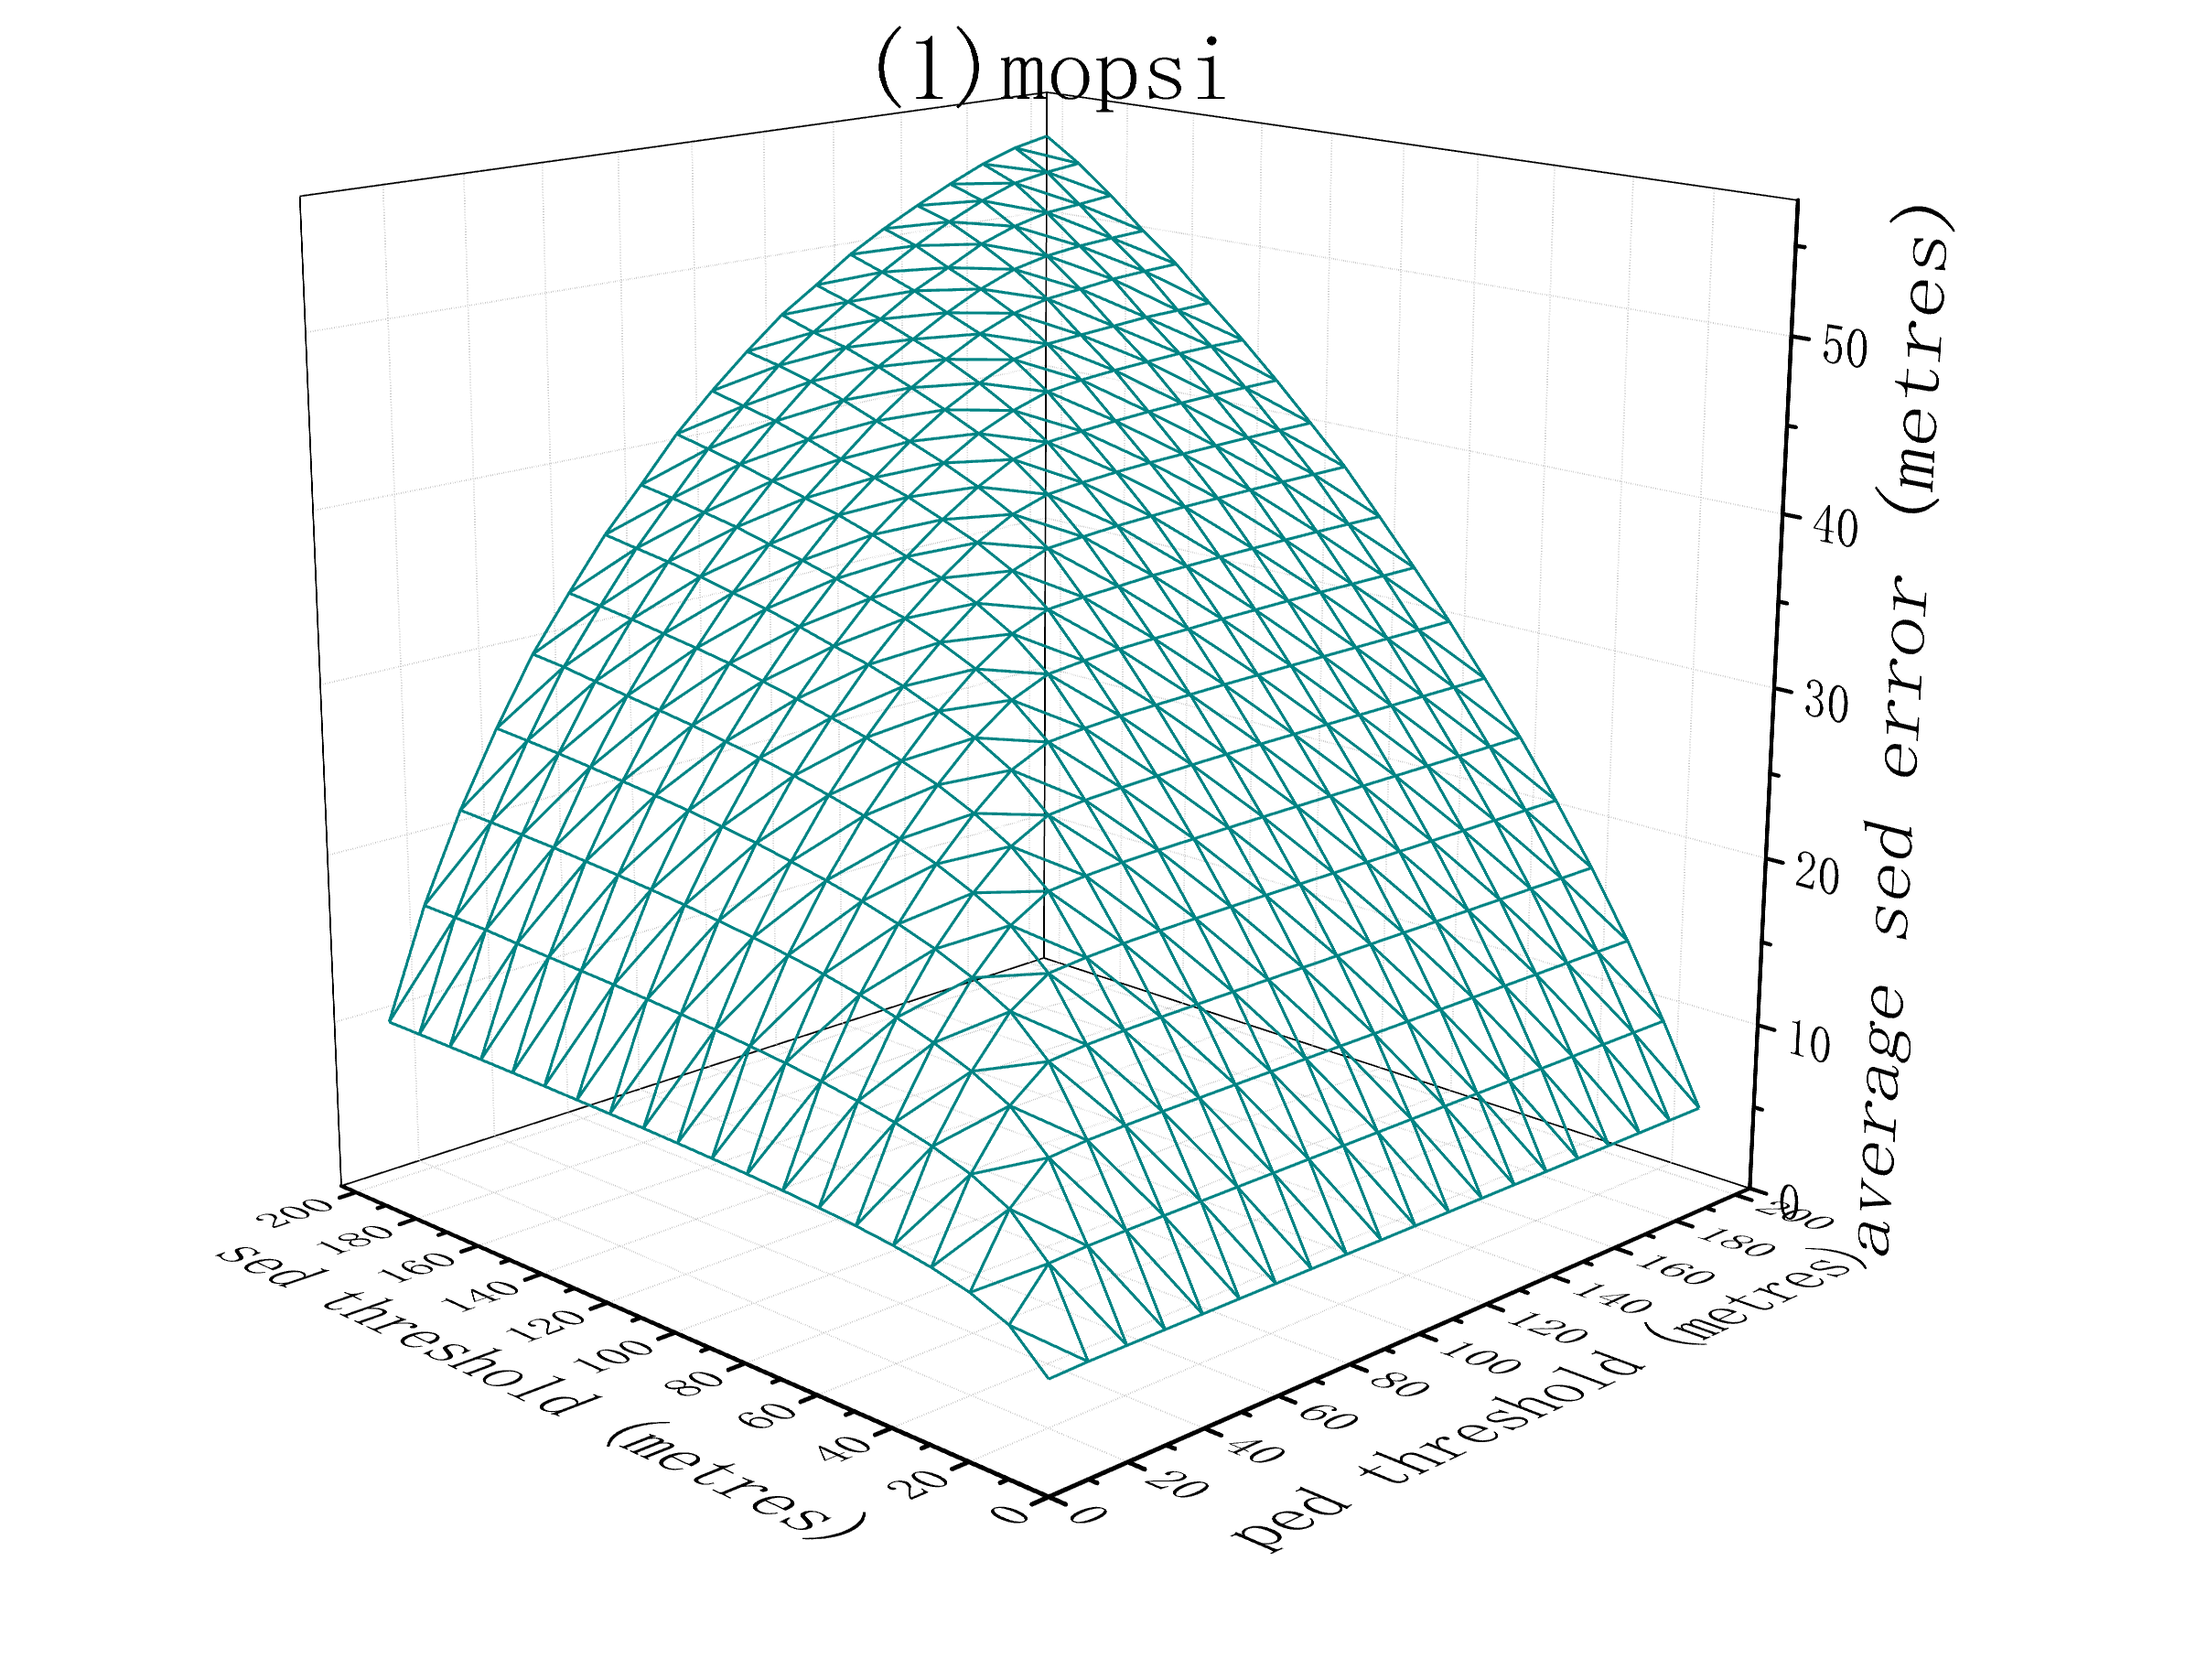
\includegraphics[scale = 0.210]{figures/Fig-BITT-mopsi-sed-error.png}\hspace{1ex}
	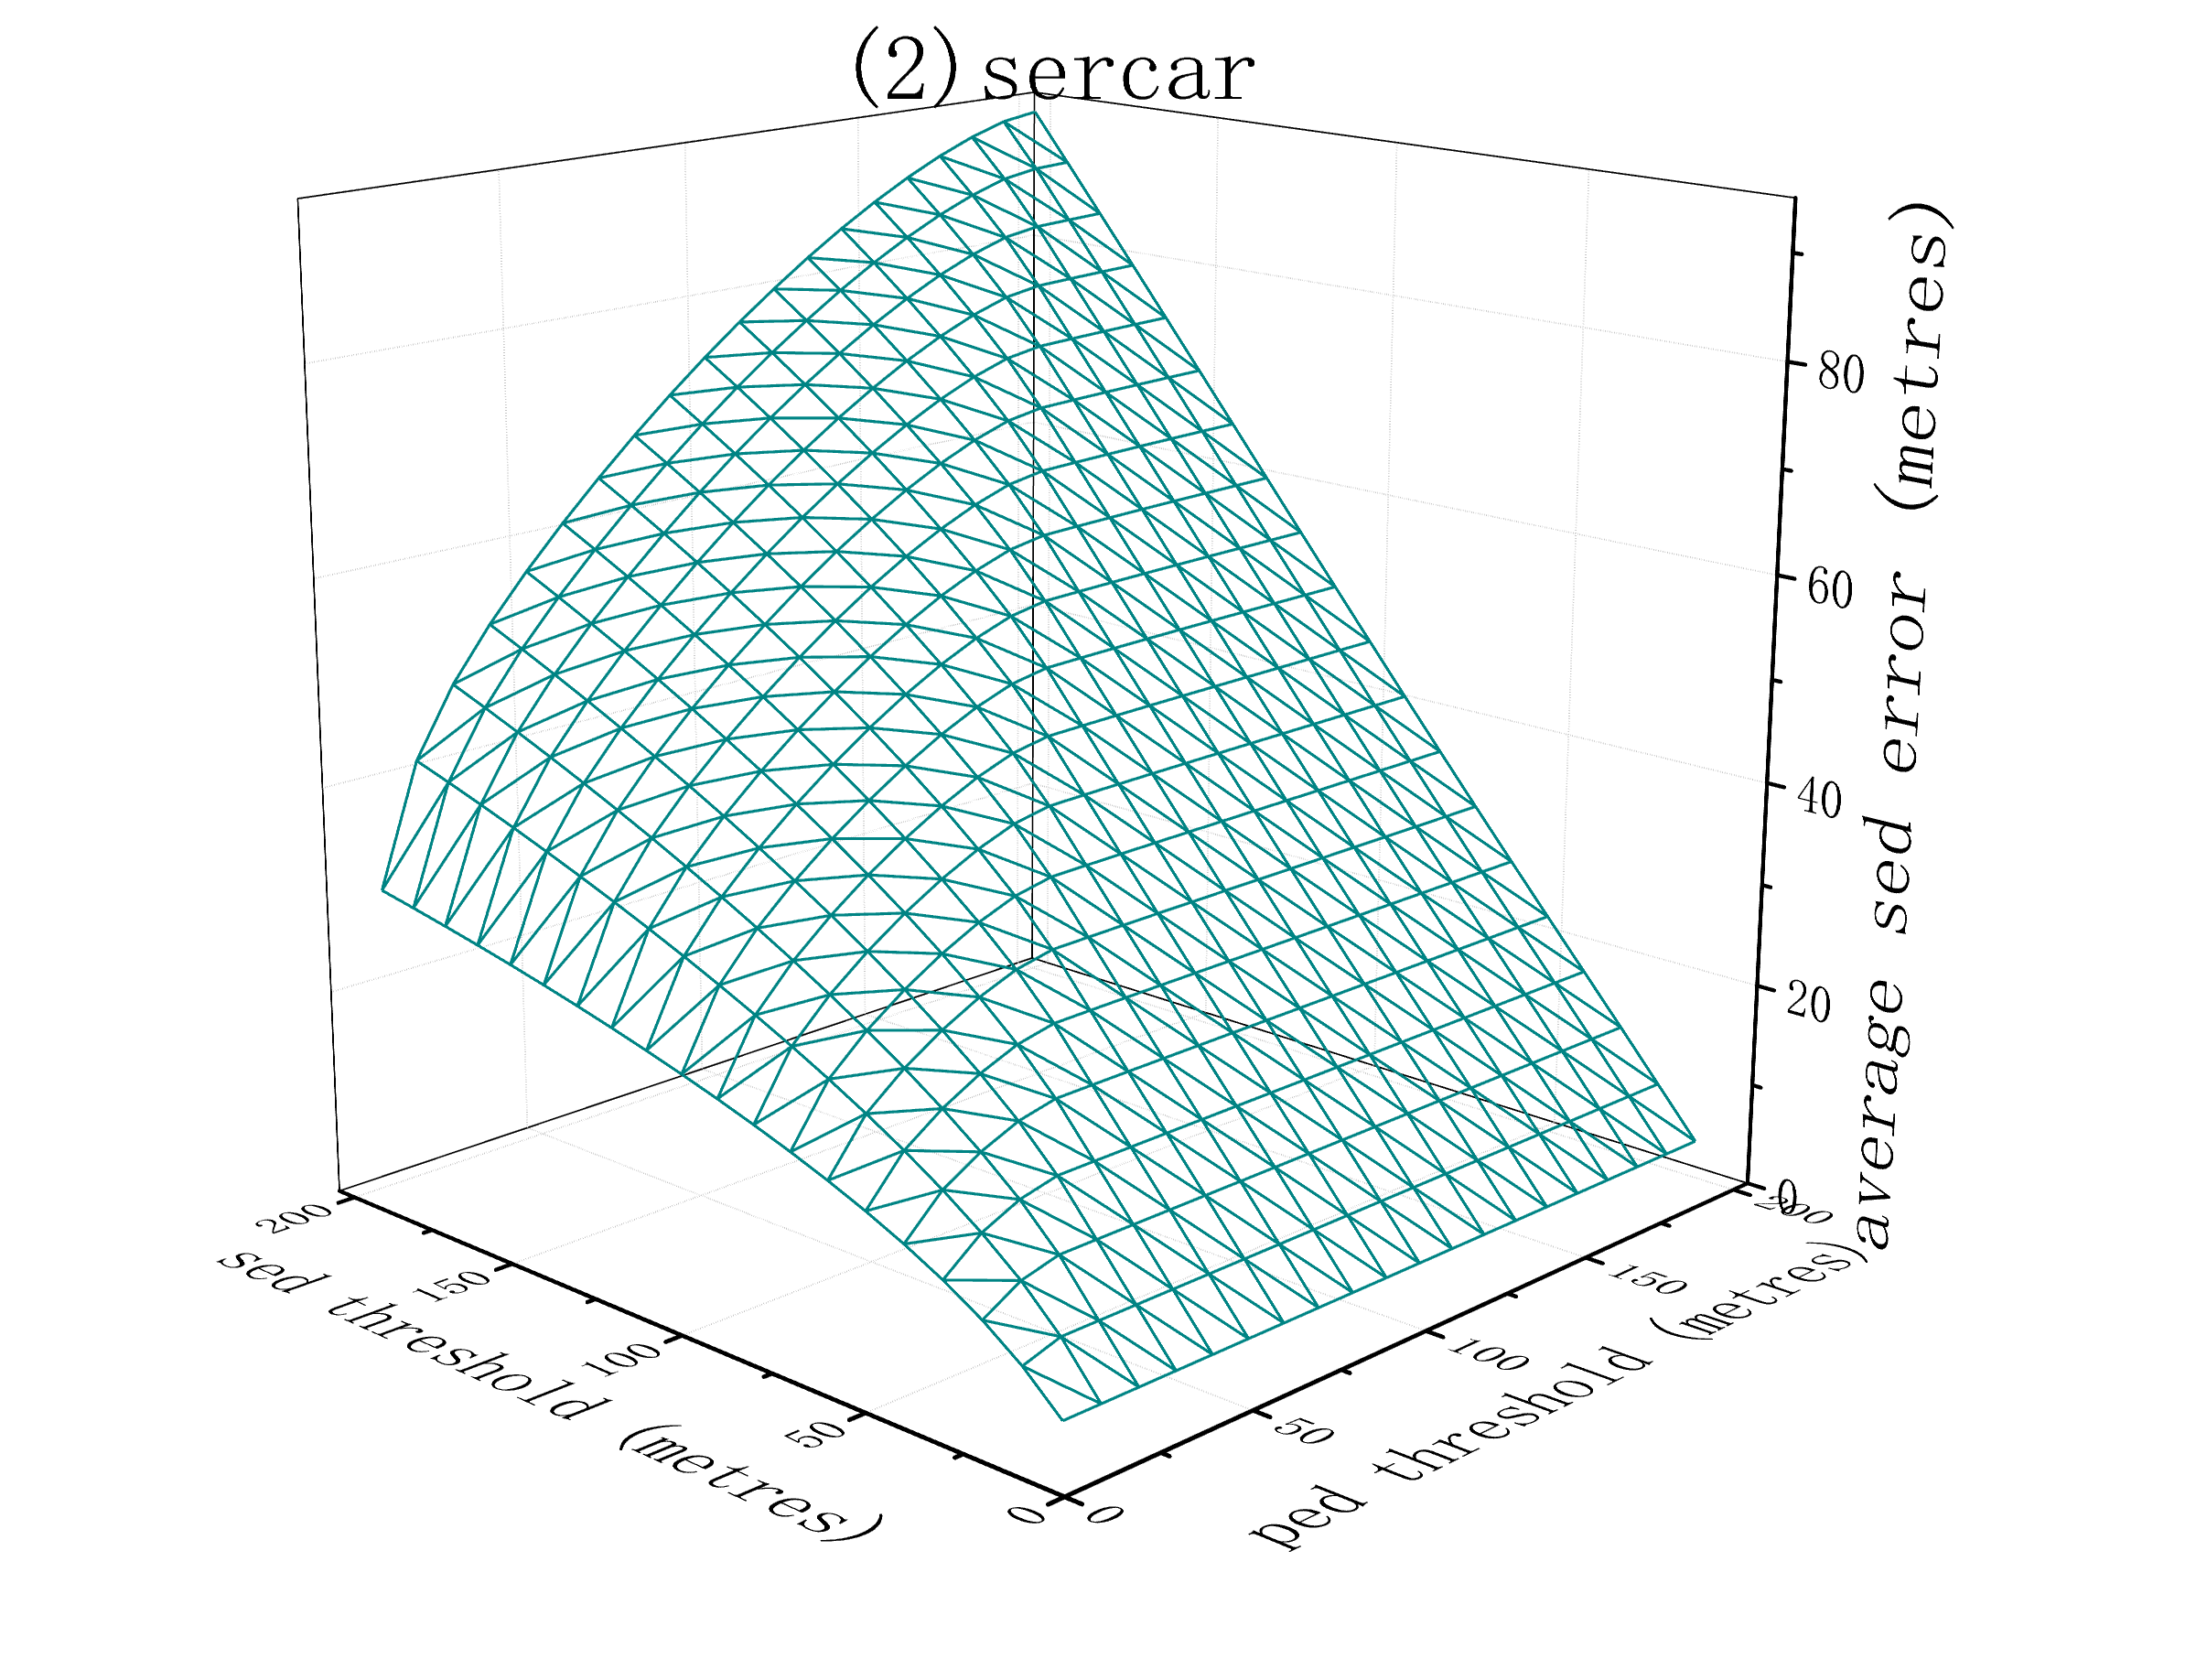
\includegraphics[scale = 0.210]{figures/Fig-BITT-sercar-sed-error.png}\hspace{1ex}
	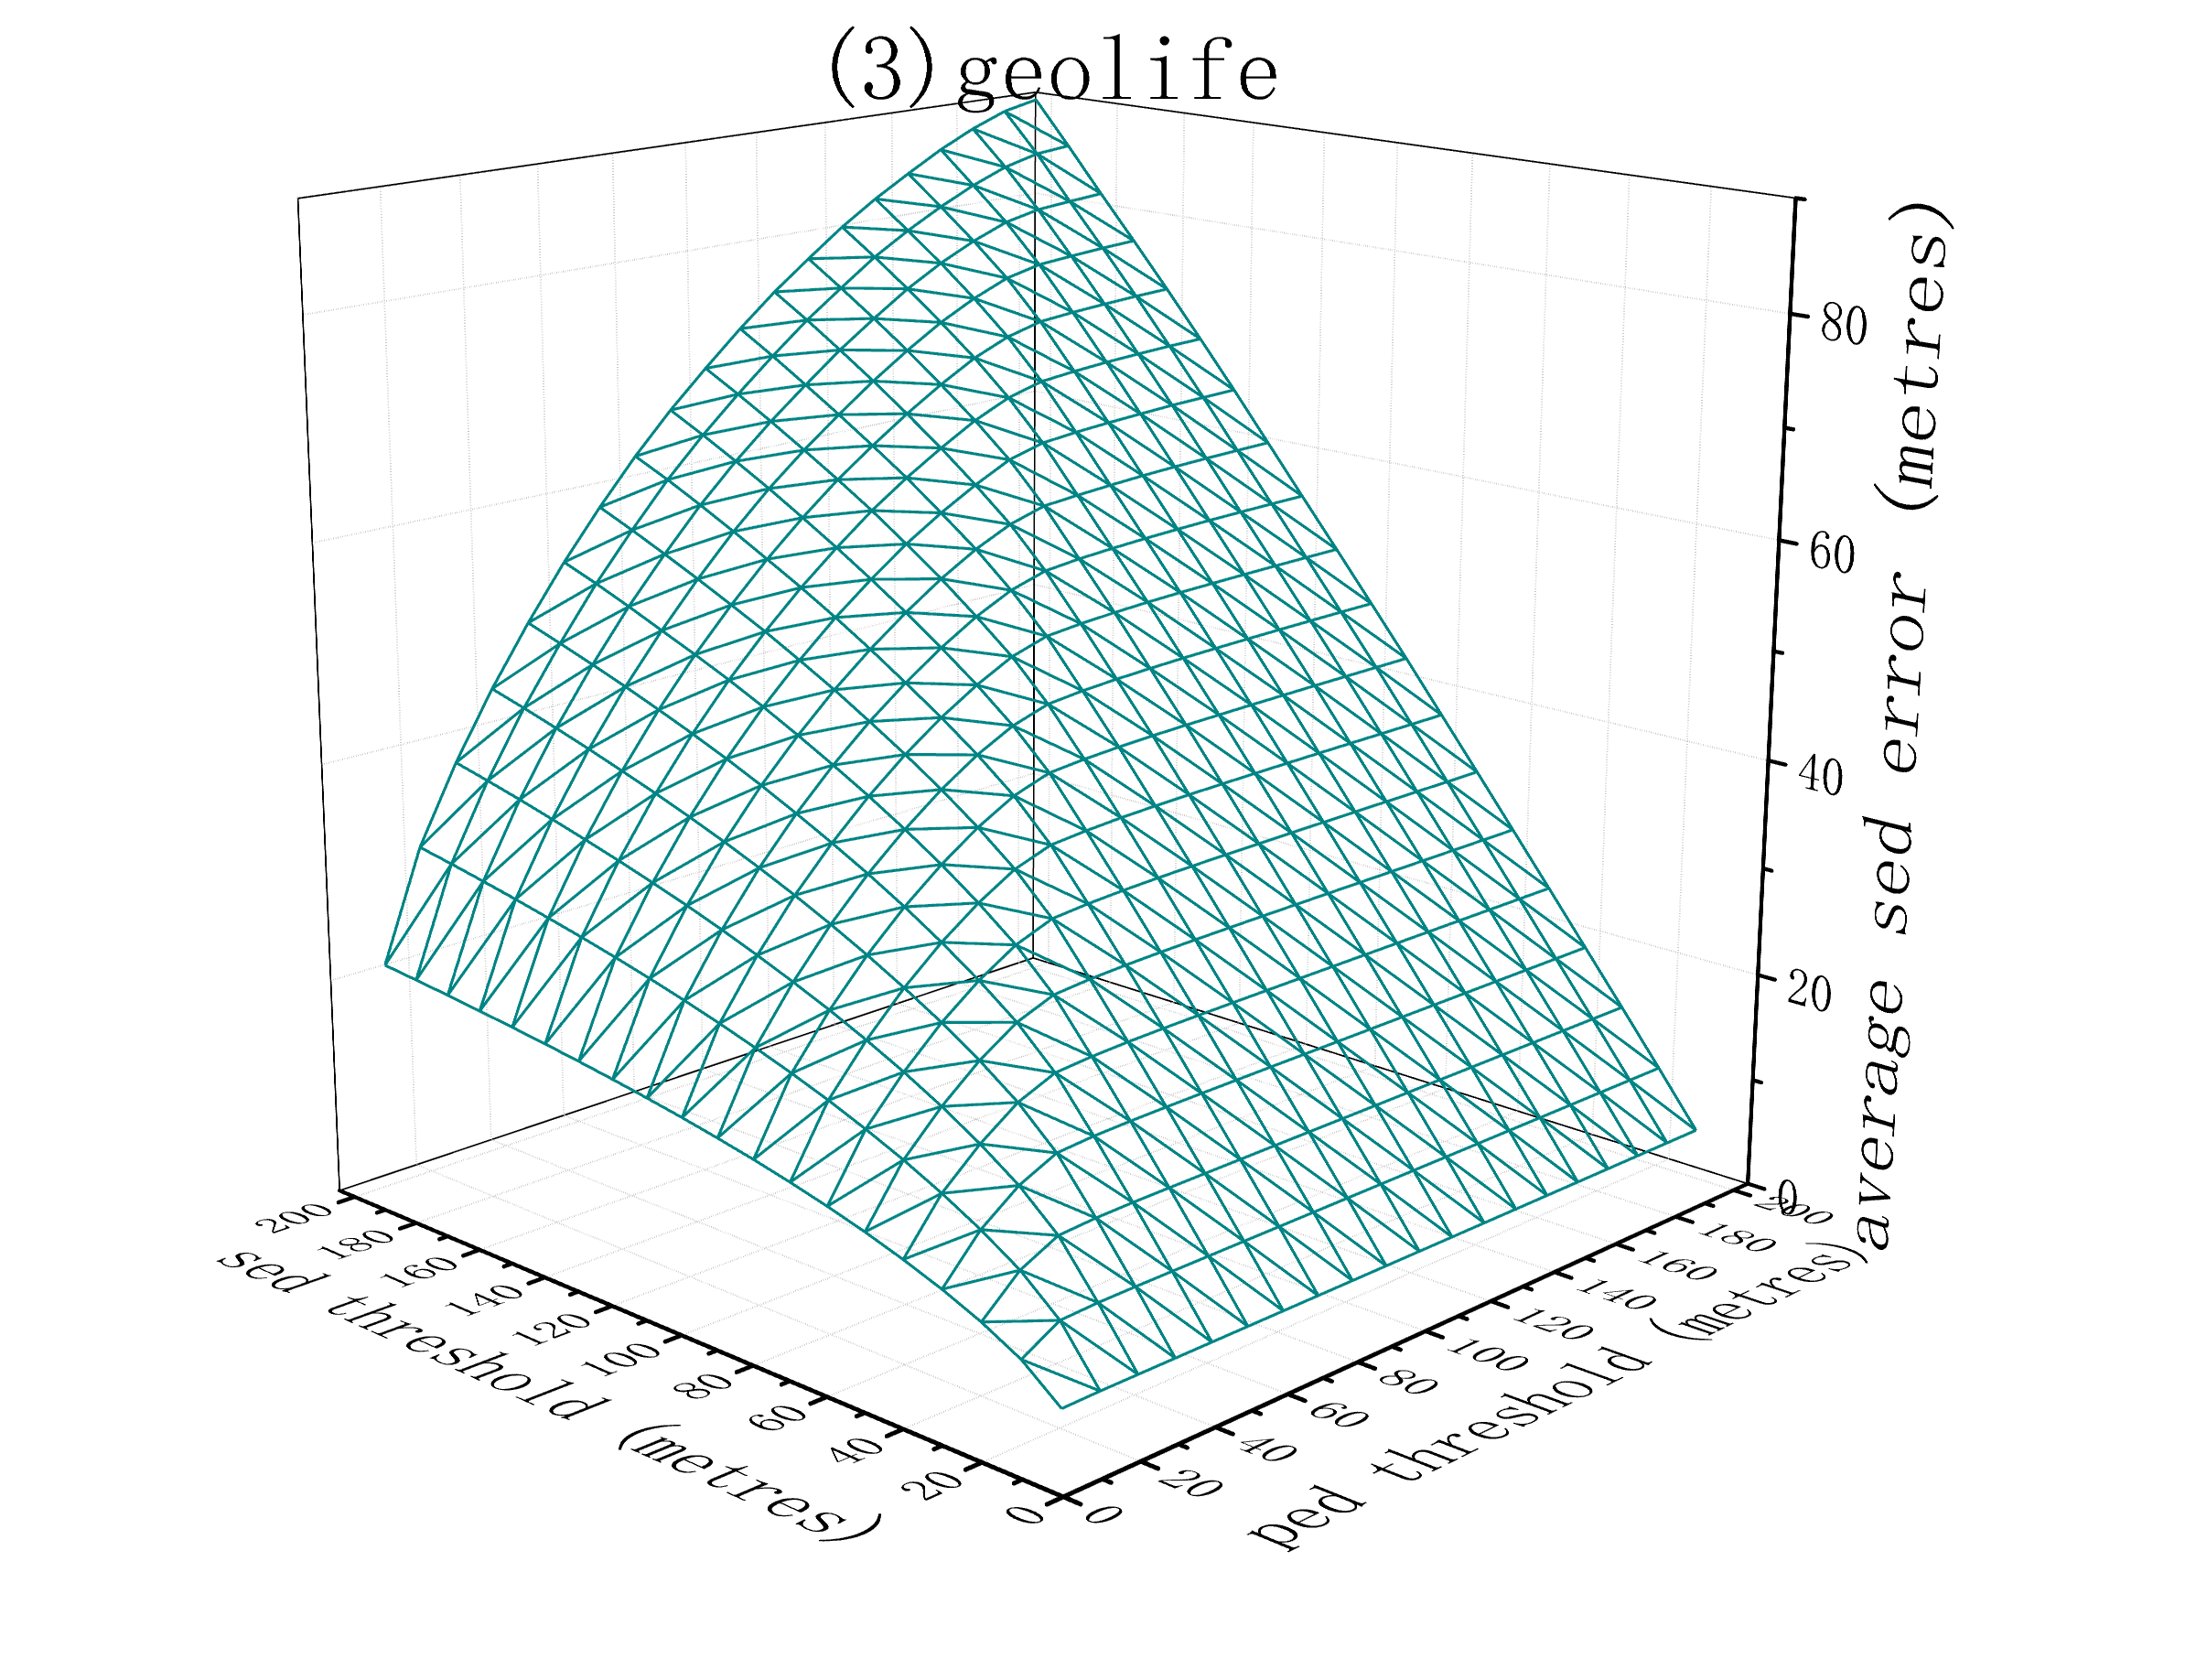
\includegraphics[scale = 0.210]{figures/Fig-BITT-geolife-sed-error.png}\hspace{1ex}
	\vspace{-2ex}
	\caption{\small Evaluation of BITT sed error: varying error bounds $\epsilon_{sed}$ and $\epsilon_{ped}$.}
	\label{fig:bitt-sed-error}
	\vspace{-1ex}
\end{figure*}



\begin{figure*}[tb!]
	\centering
	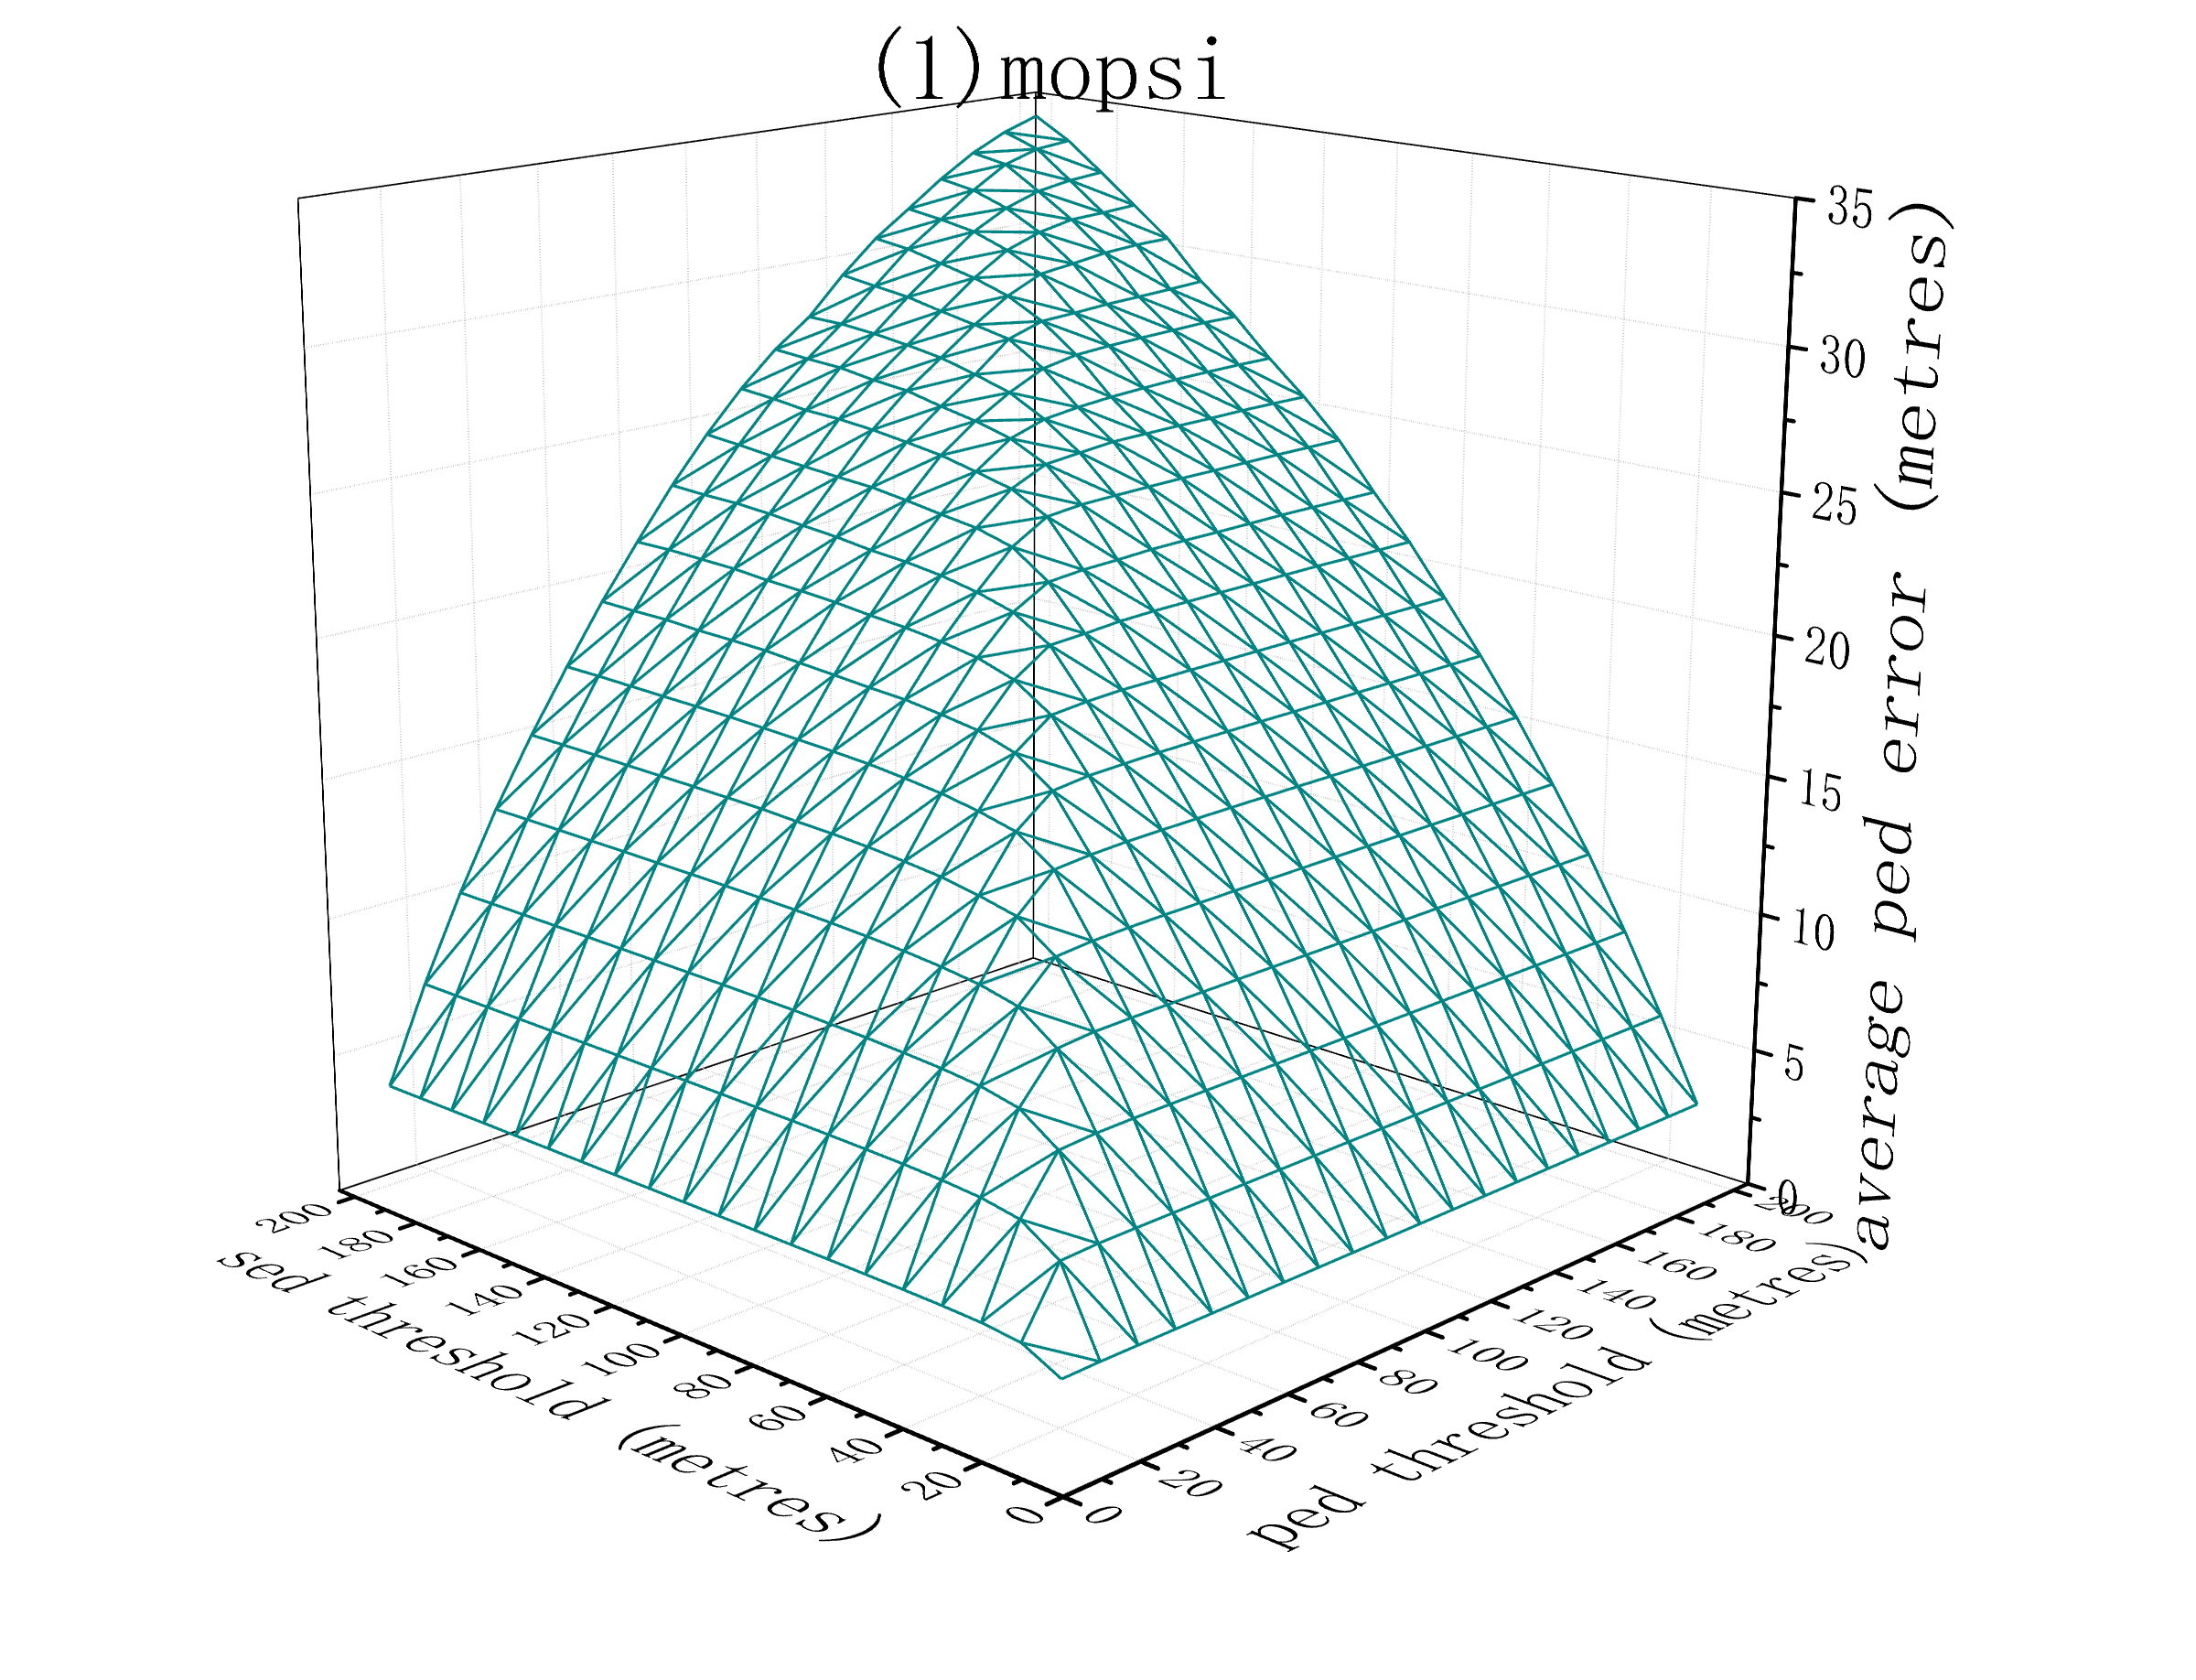
\includegraphics[scale = 0.210]{figures/Fig-BITT-mopsi-ped-error.png}\hspace{1ex}
	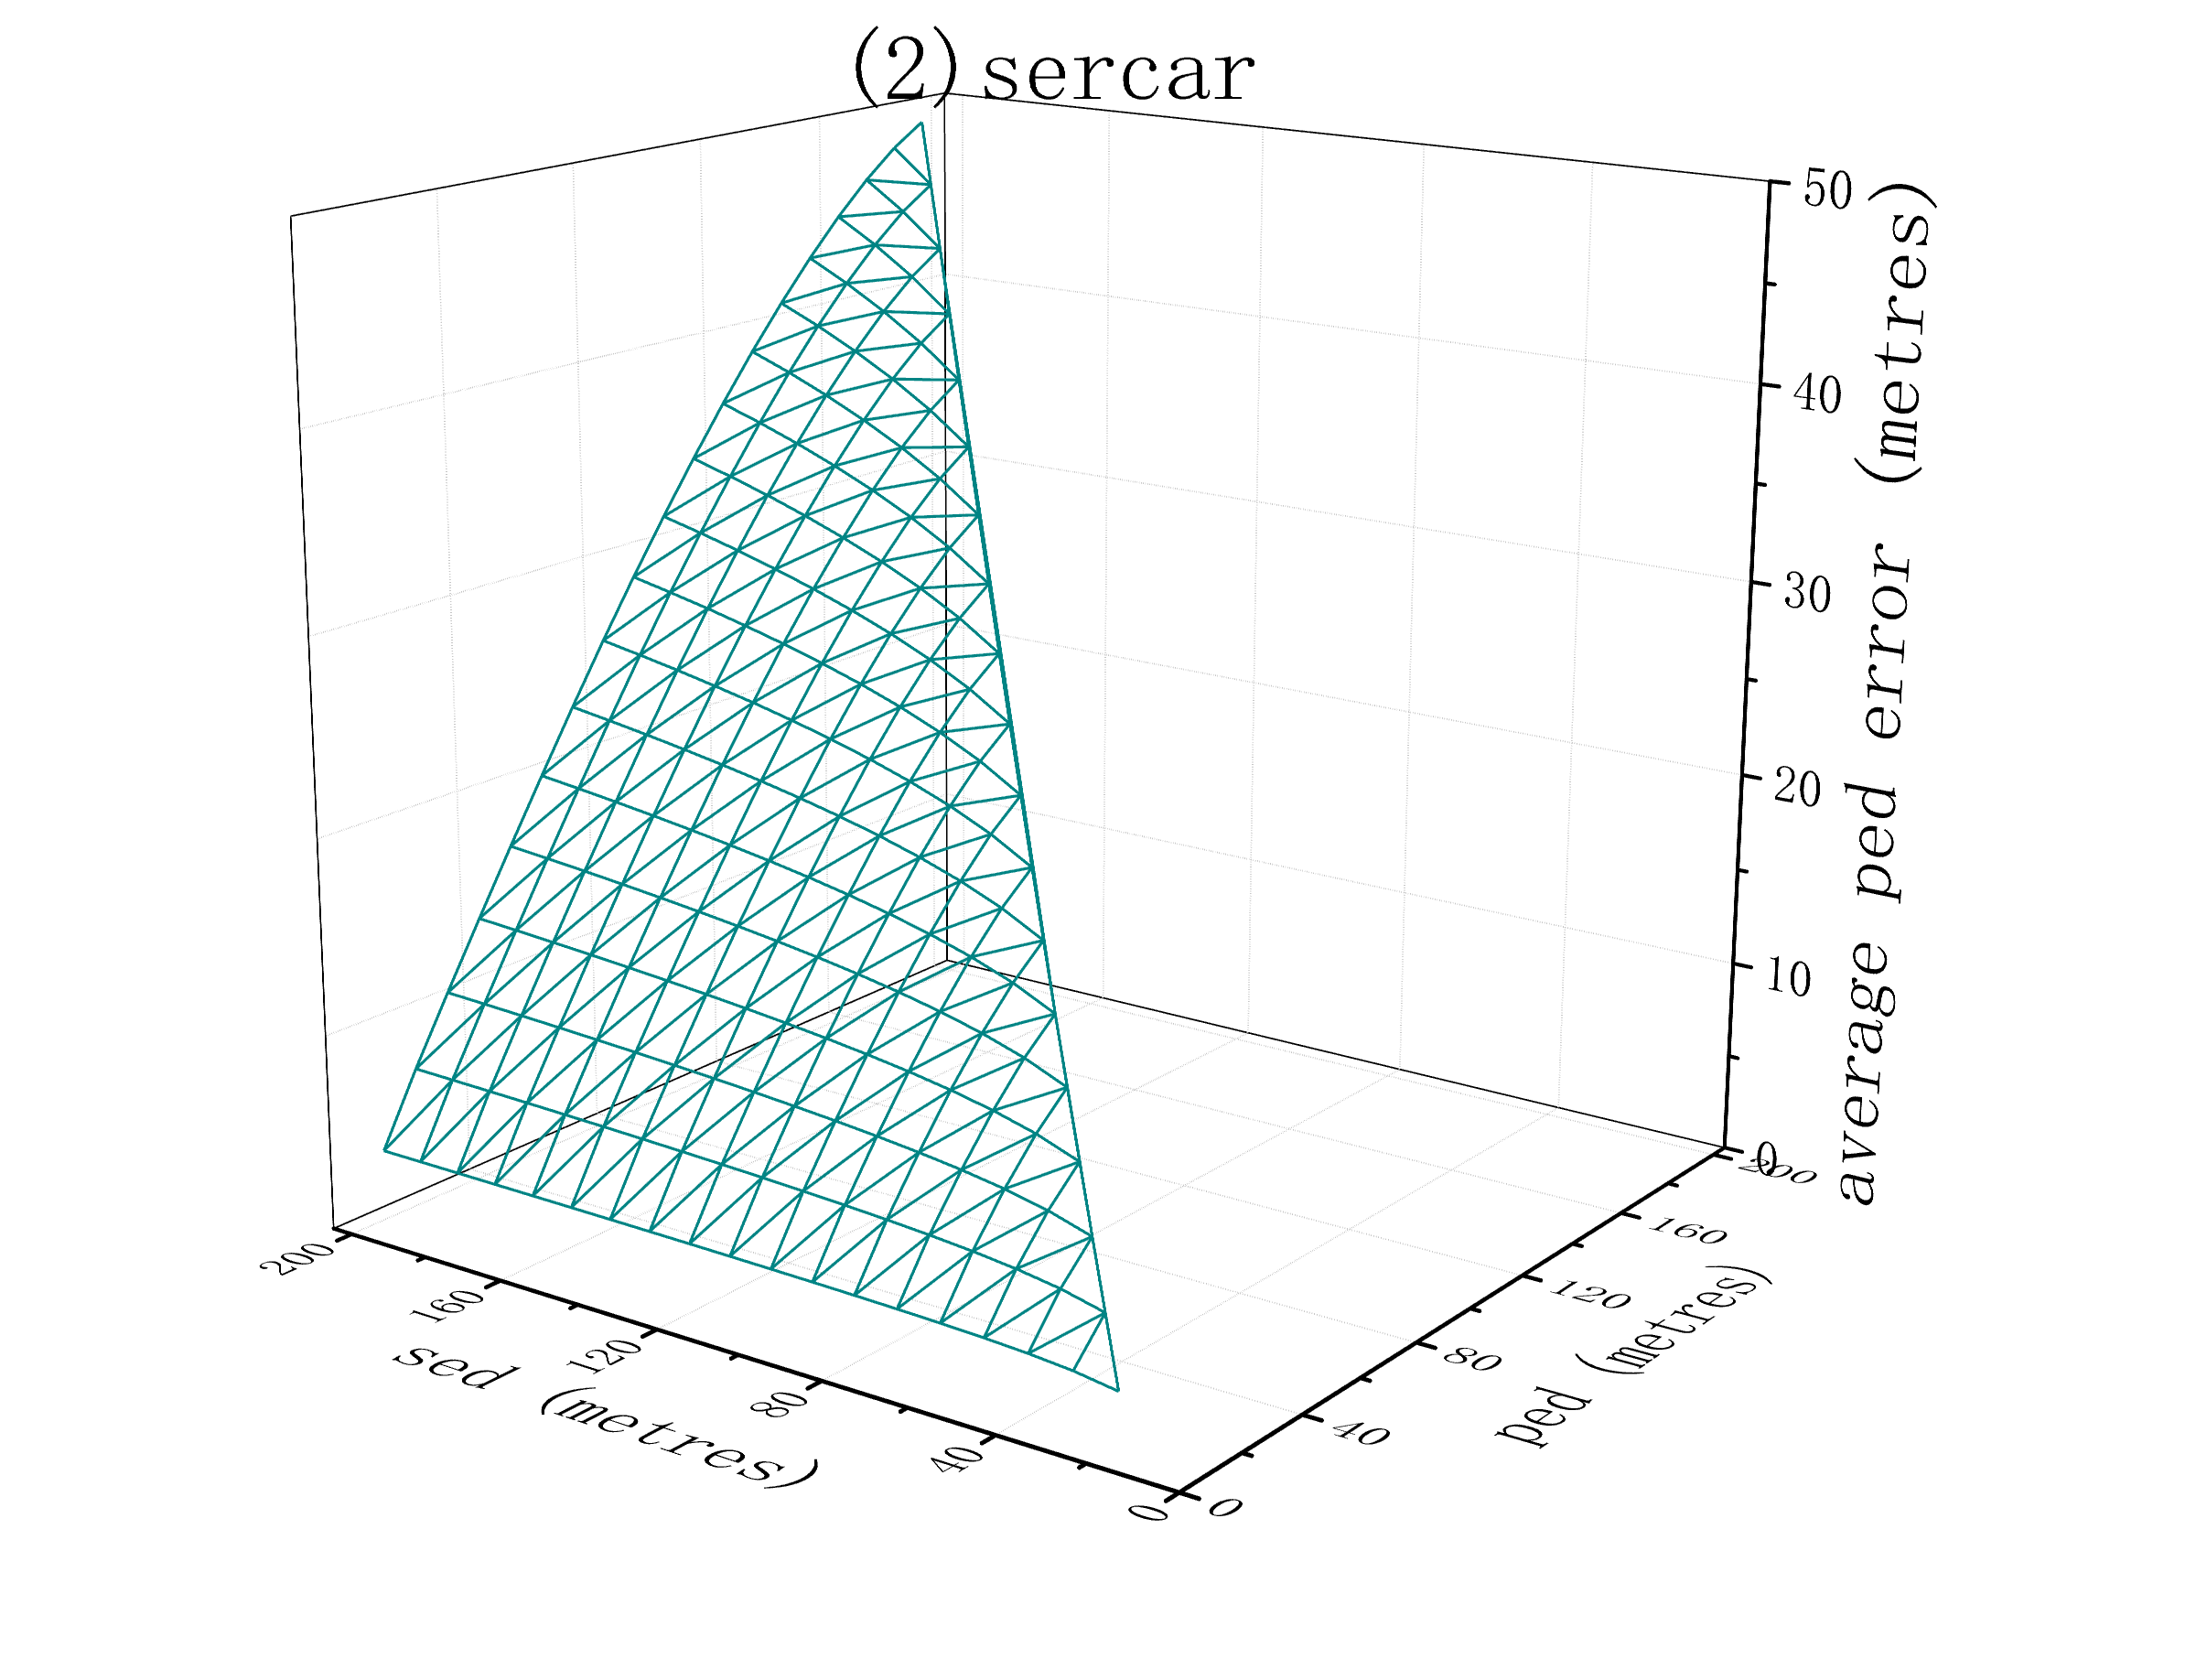
\includegraphics[scale = 0.210]{figures/Fig-BITT-sercar-ped-error.png}\hspace{1ex}
	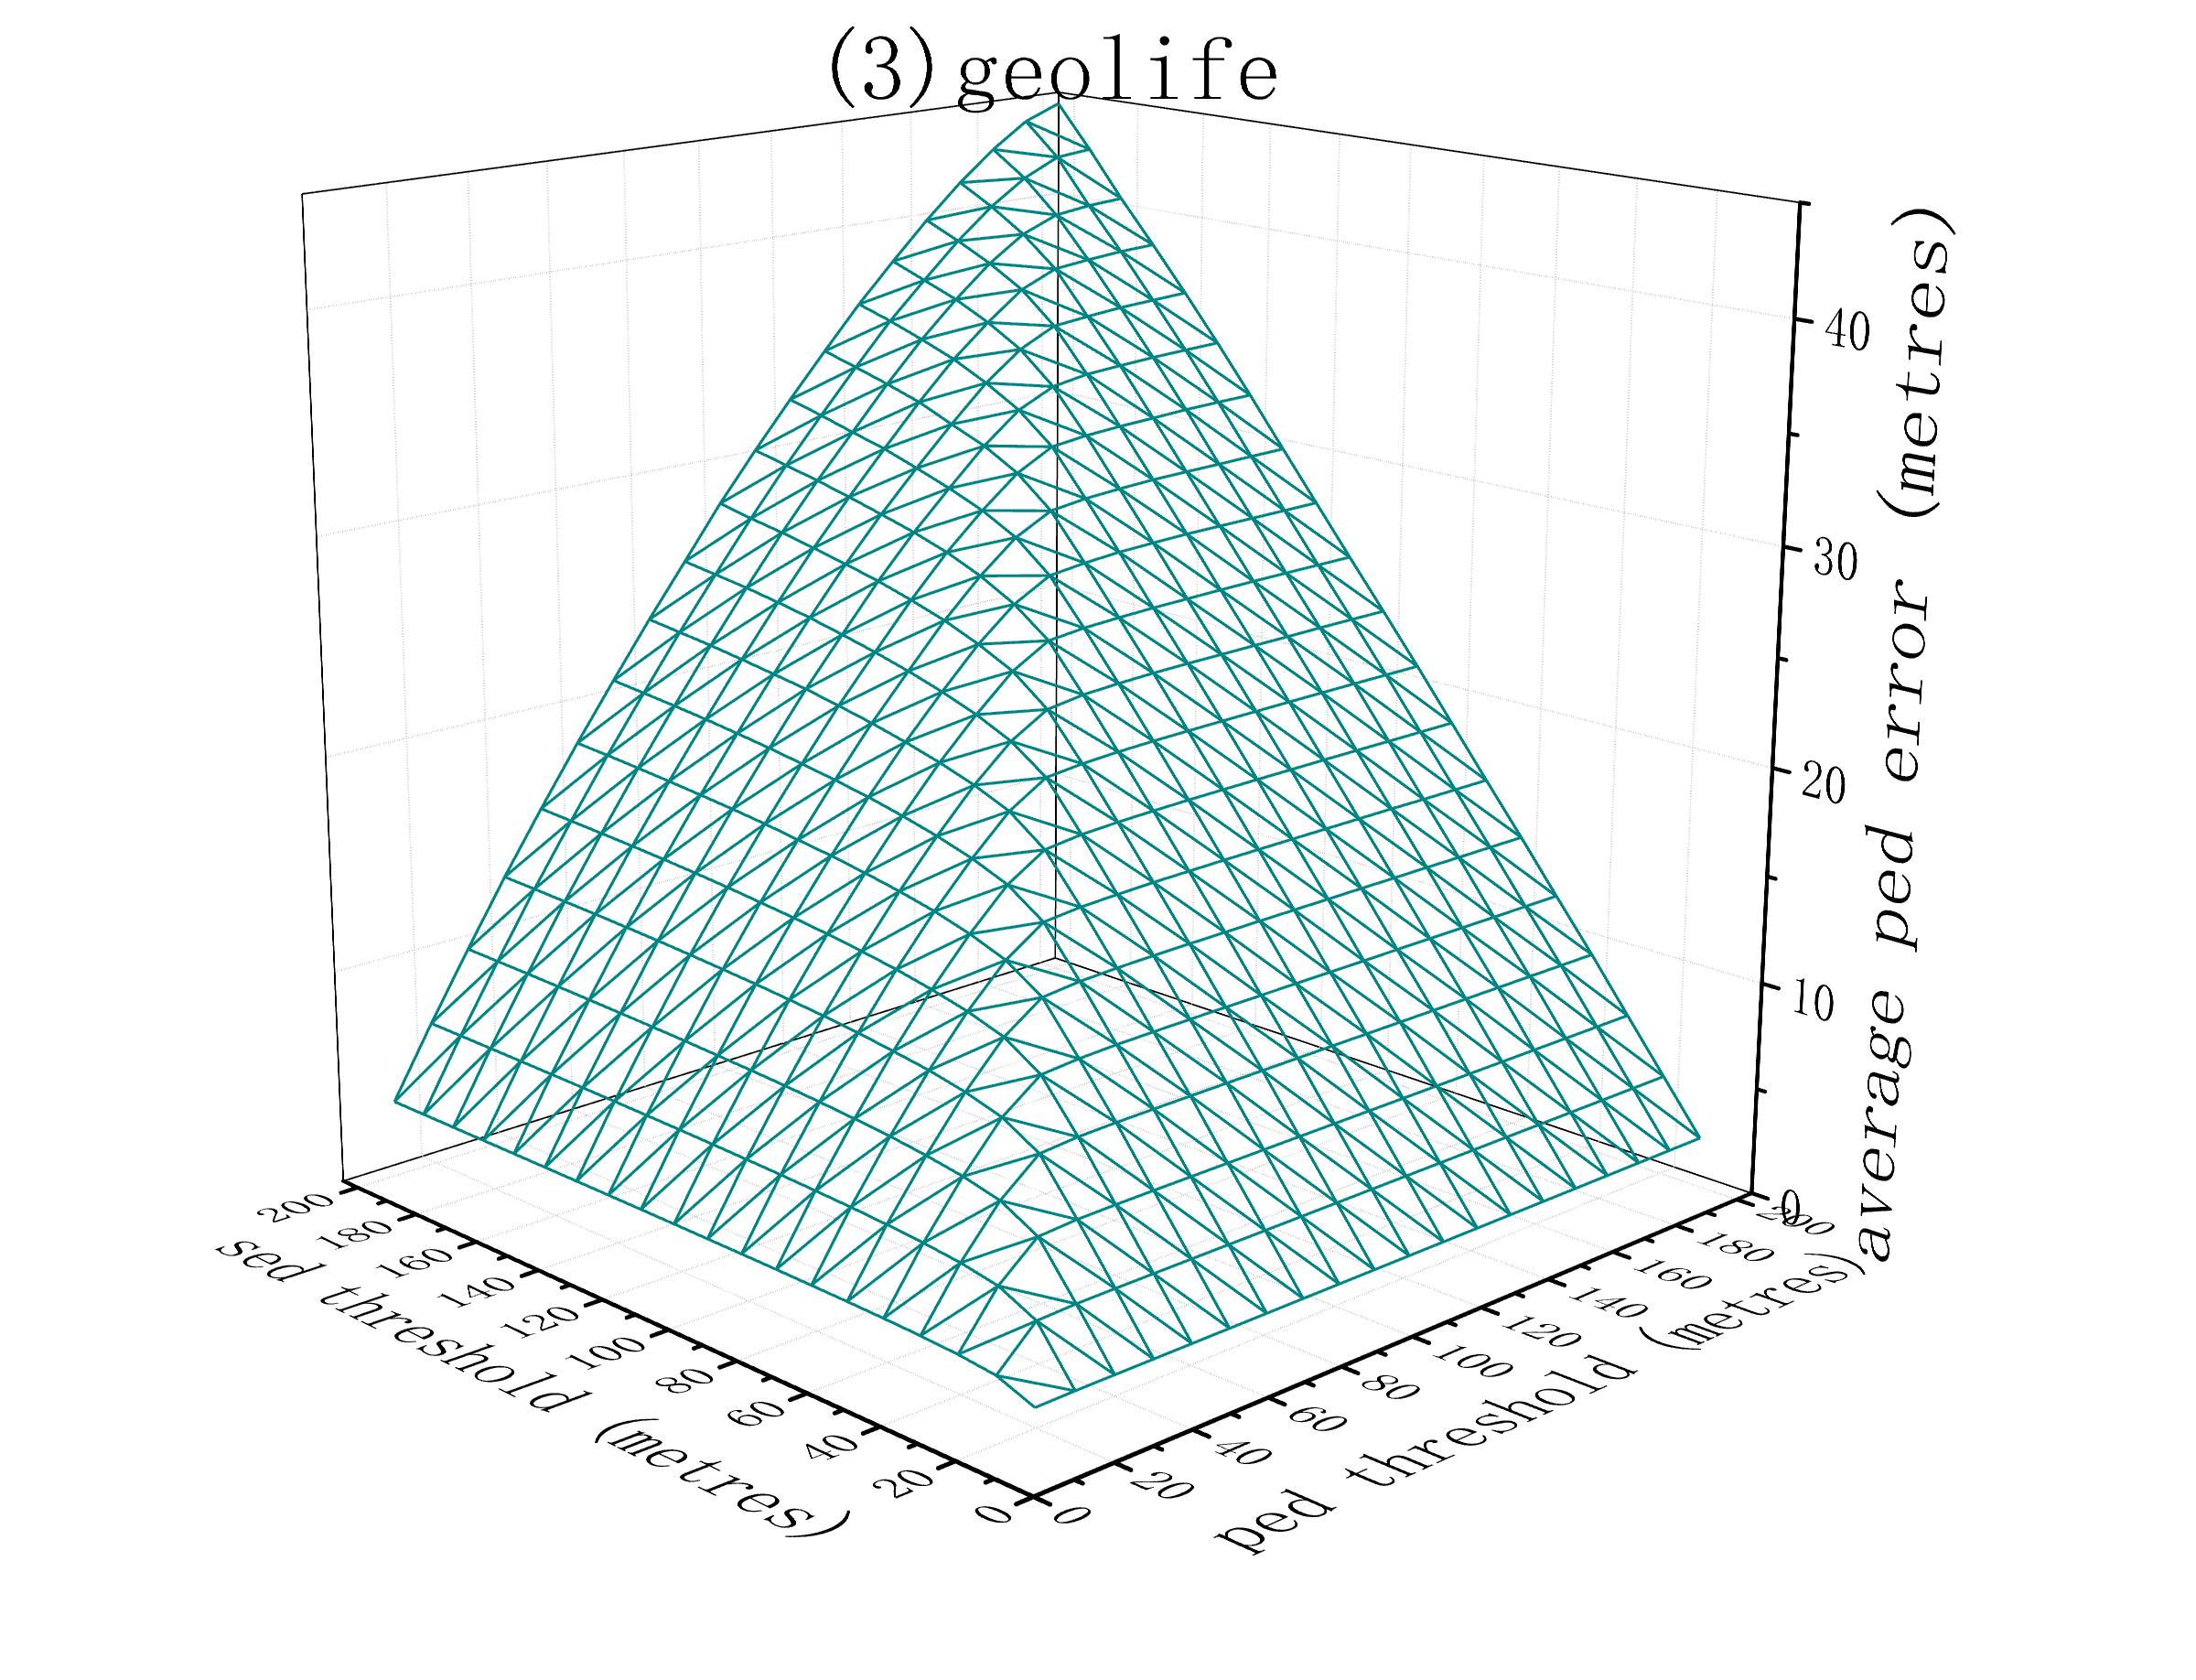
\includegraphics[scale = 0.210]{figures/Fig-BITT-geolife-ped-error.png}\hspace{1ex}
	\vspace{-2ex}
	\caption{\small Evaluation of BITT ped error: varying error bounds $\epsilon_{sed}$ and $\epsilon_{ped}$.}
	\label{fig:bitt-ped-error}
	\vspace{-1ex}
\end{figure*}



\subsubsection{Evaluation of~algorithm \bitt}
%%%%%%%%%%%% messages
This section test the impacts of \ped and \sed (\ie the shapes of rectangle-like areas) on \bitt. We varied $\epsilon_{sed}$ and $\epsilon_{ped}$ from $10$ meters to $200$ meters on the entire three datasets, respectively. The results are reported in Figures~\ref{fig:bitt-total-message}, \ref{fig:bitt-compression-ratio}, \ref{fig:bitt-sed-error} and \ref{fig:bitt-ped-error}.

\stitle{Messages}.
We can see that the total messages decreases with the increase of $\epsilon_{sed}$ and $\epsilon_{ped}$. This is because as the tracking area becomes larger, \bitt is more tolerant of the movement range of the moving object, so fewer messages are transmitted.

\stitle{Compression ratios}.
%%%%%%%%%%%%%%%%%% compression ratios
\ni (1) When increasing $\epsilon_{sed}$ and $\epsilon_{ped}$, the compression ratios of all these algorithms decrease on all datasets.


\stitle{Average errors.}






\subsubsection{Comparing algorithms \bitt, \sitt and \citt with \ldrh and \grts.}
This section compares our algorithms \citt, \sitt and \bitt with algorithms \ldrh and \grts.
We varied the error bound (either $\epsilon_{sed}$ or $\epsilon_{ped}$) from $10$ meters to $200$ meters on the entire three datasets, respectively. 
\myred{For \bitt, the we fixed $\epsilon_{ped}$ used by \bitt is 0.9 times the $\epsilon_{ped}$ used by \sitt, and the $\epsilon_{sed}$ is 1.7 times the $\epsilon_{sed}$ used by \citt, \grts and \ldrh.}
%
The results are reported in Figures~\ref{fig:total-message}, \ref{fig:speed-message},\ref{fig:compression-ratio}, \ref{fig:sed-error}, \ref{fig:ped-error} and \ref{fig:running-time}.


\begin{figure*}[tb!]
	\centering
	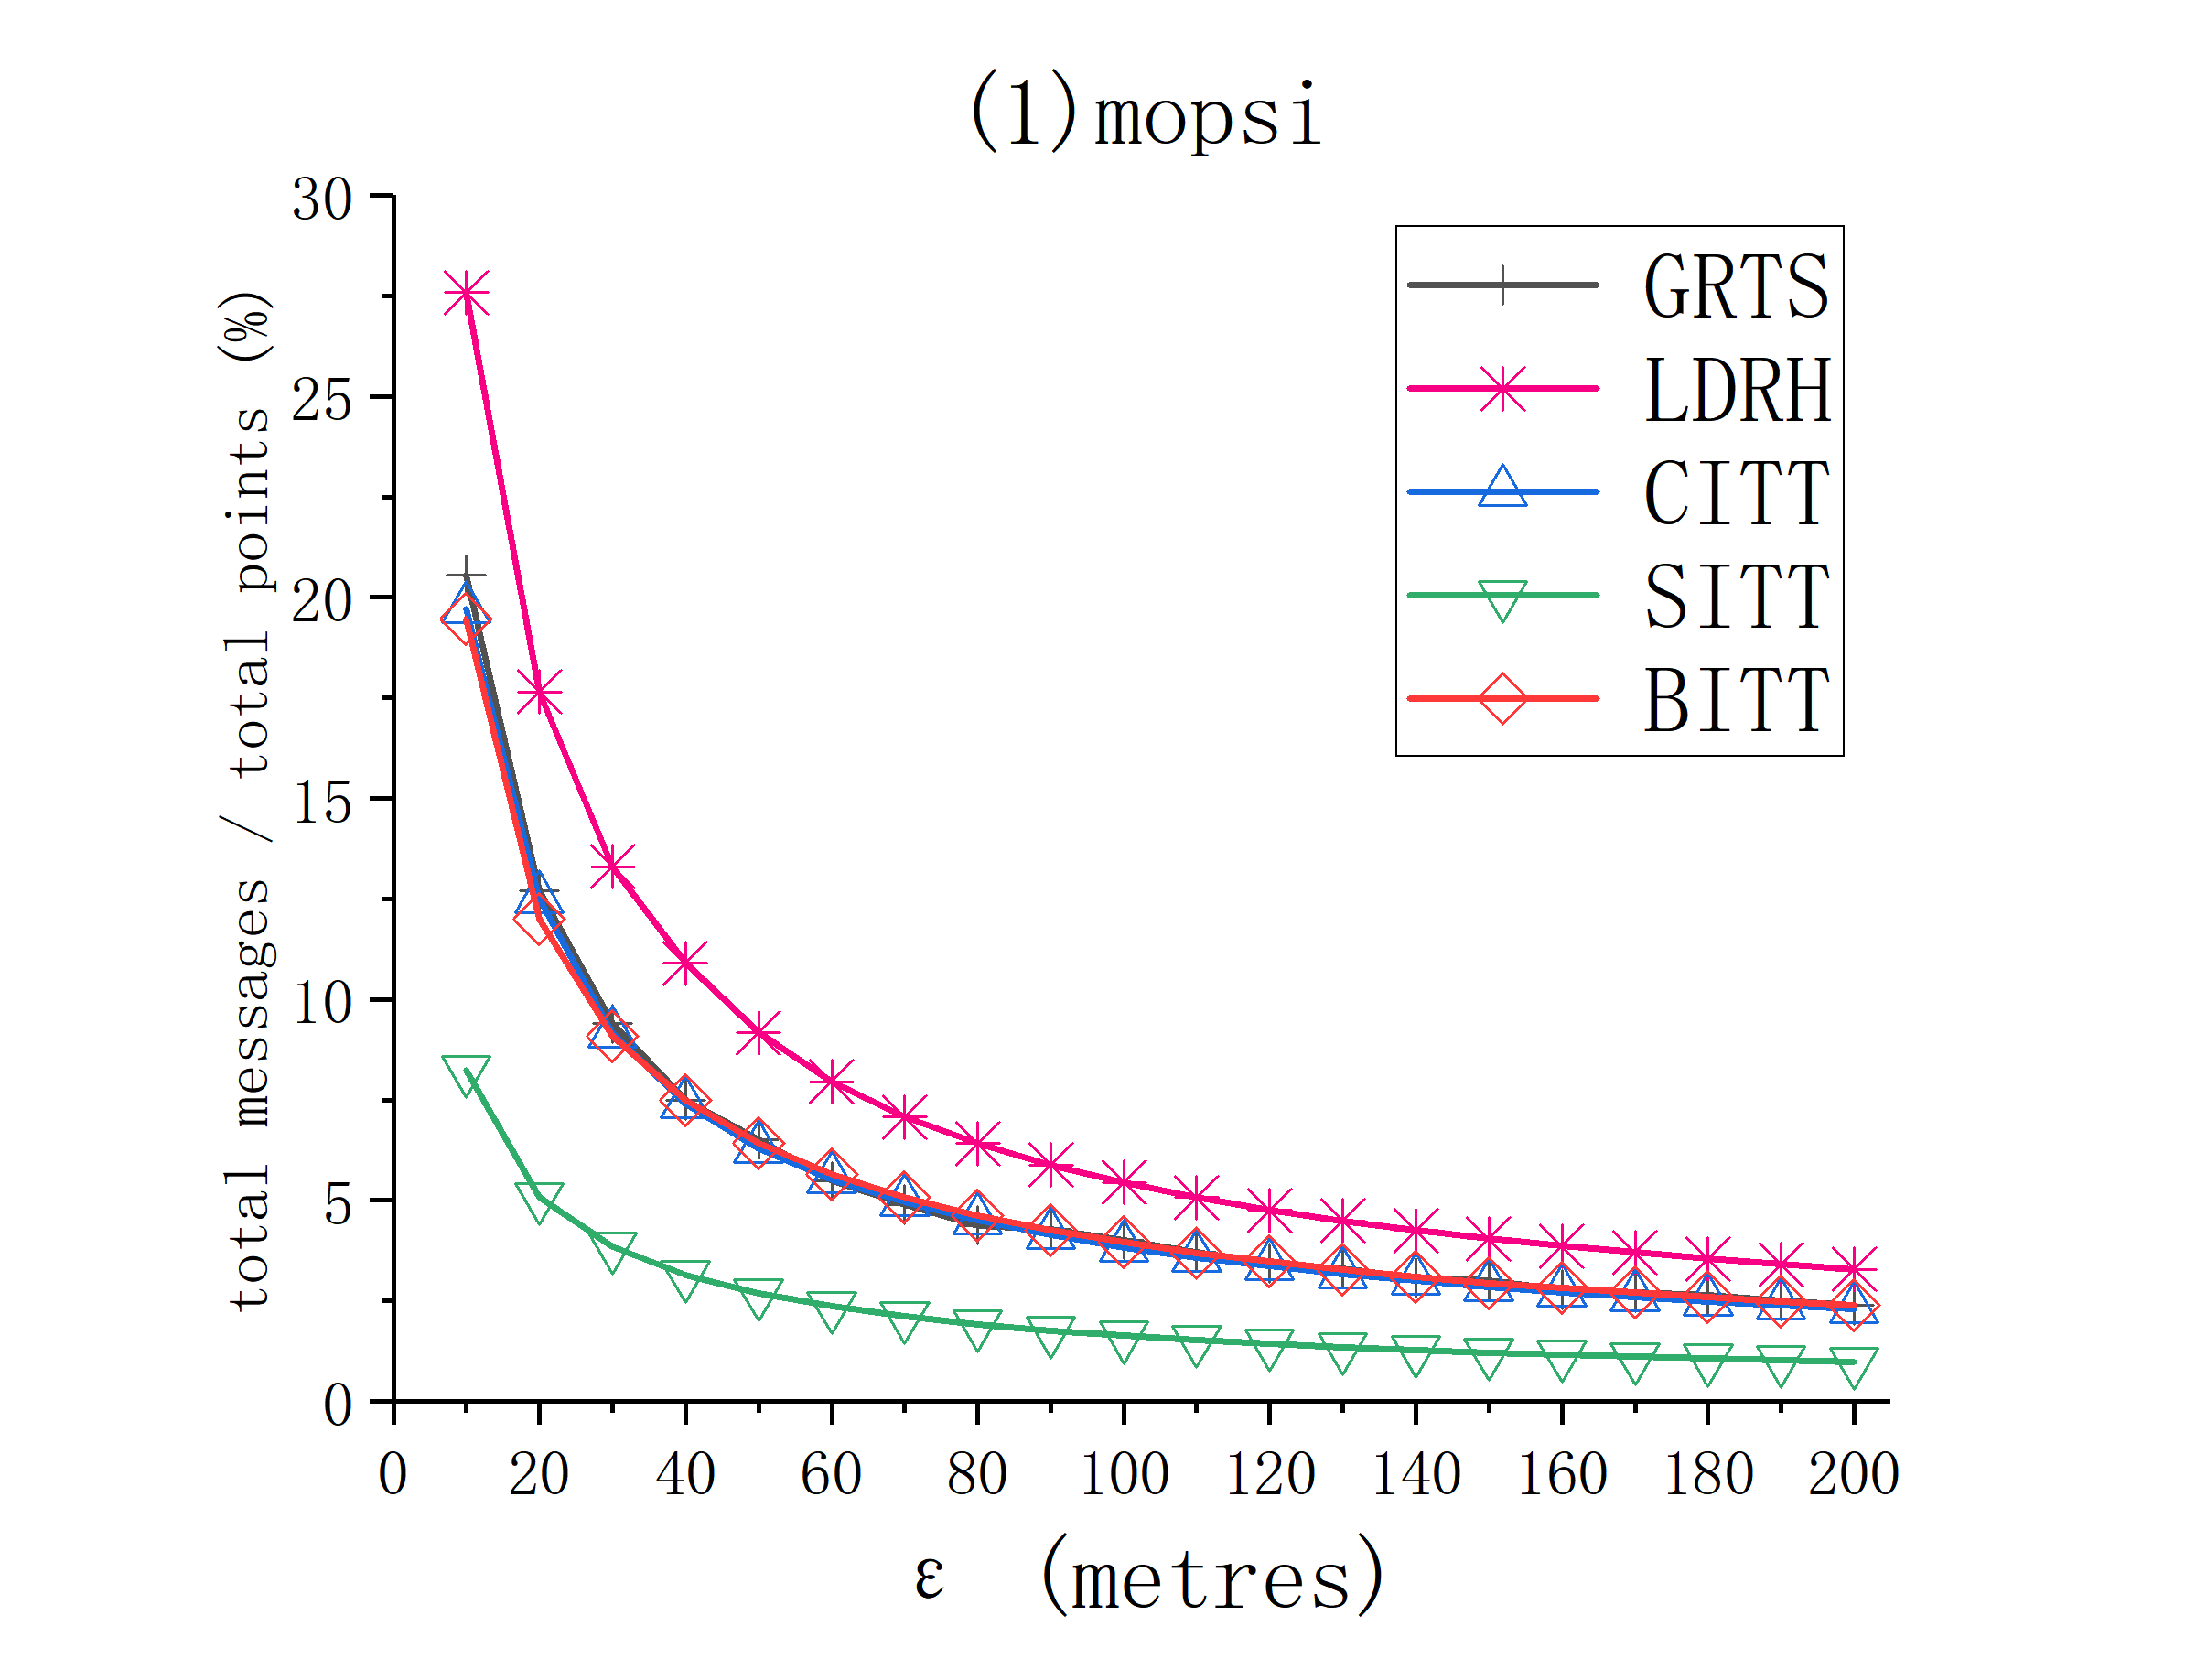
\includegraphics[scale = 0.210]{figures/Fig-mopsi-total-messages.png}\hspace{1ex}
	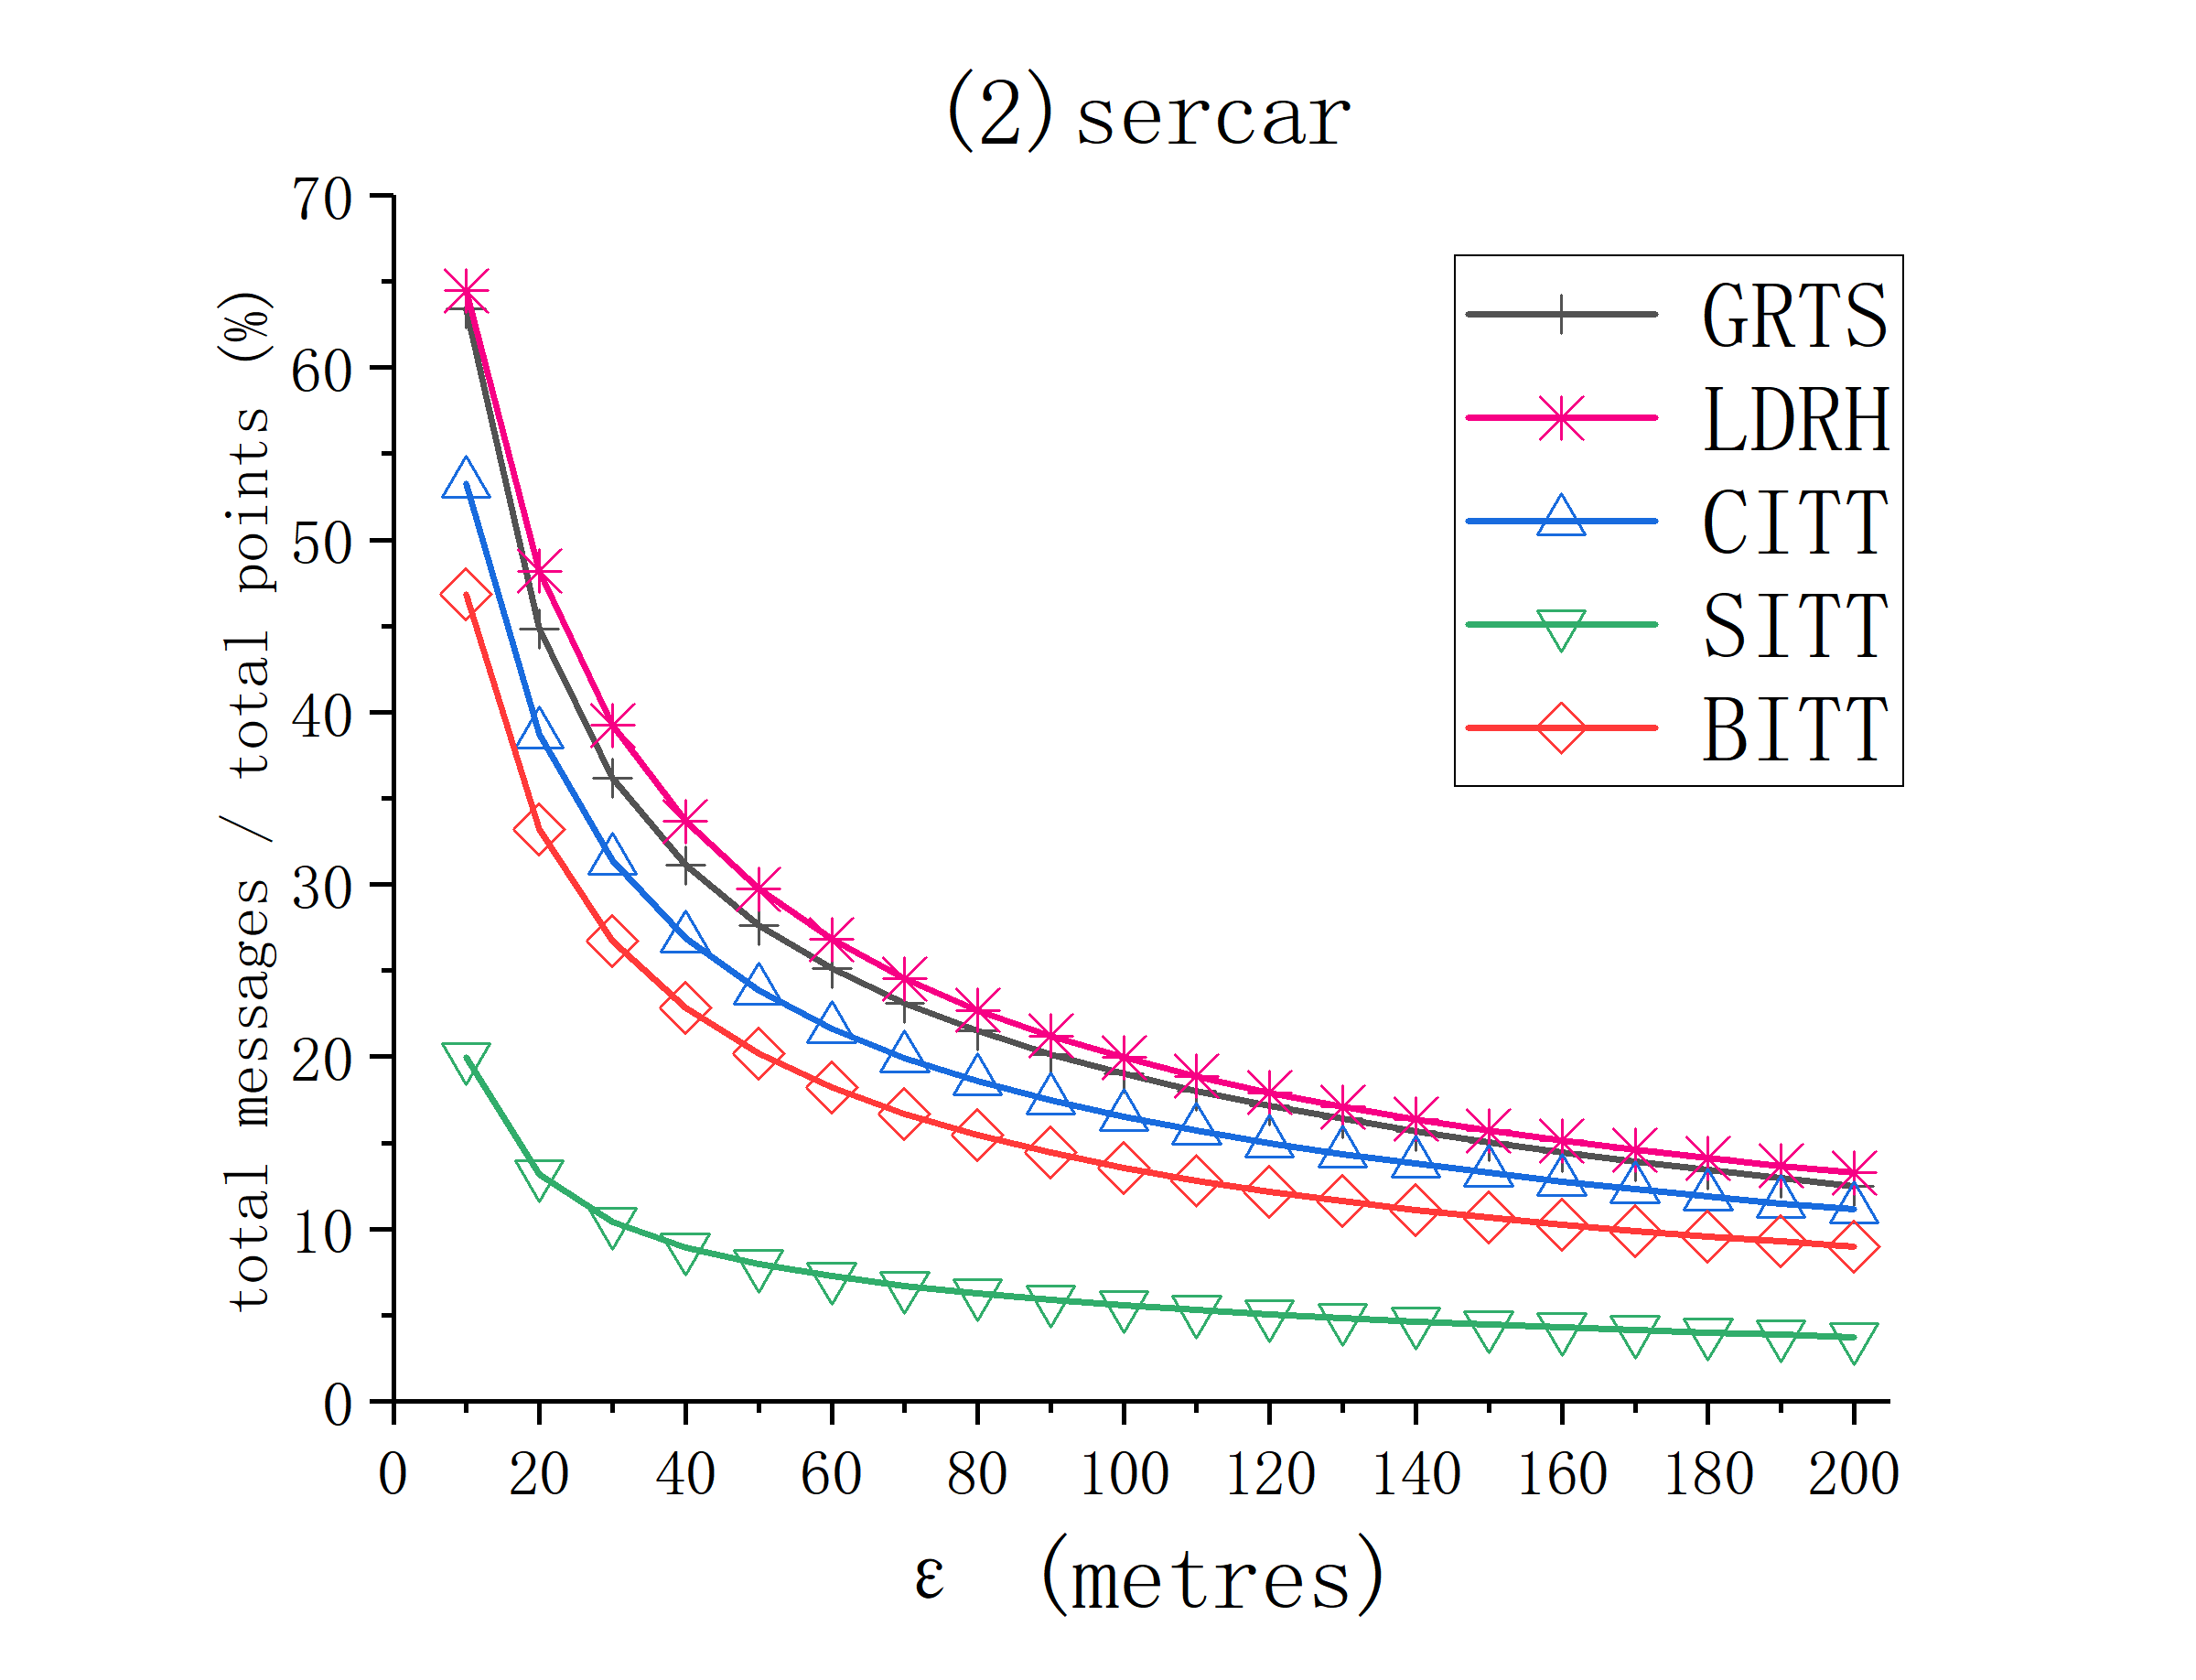
\includegraphics[scale = 0.210]{figures/Fig-sercar-total-messages.png}\hspace{1ex}
	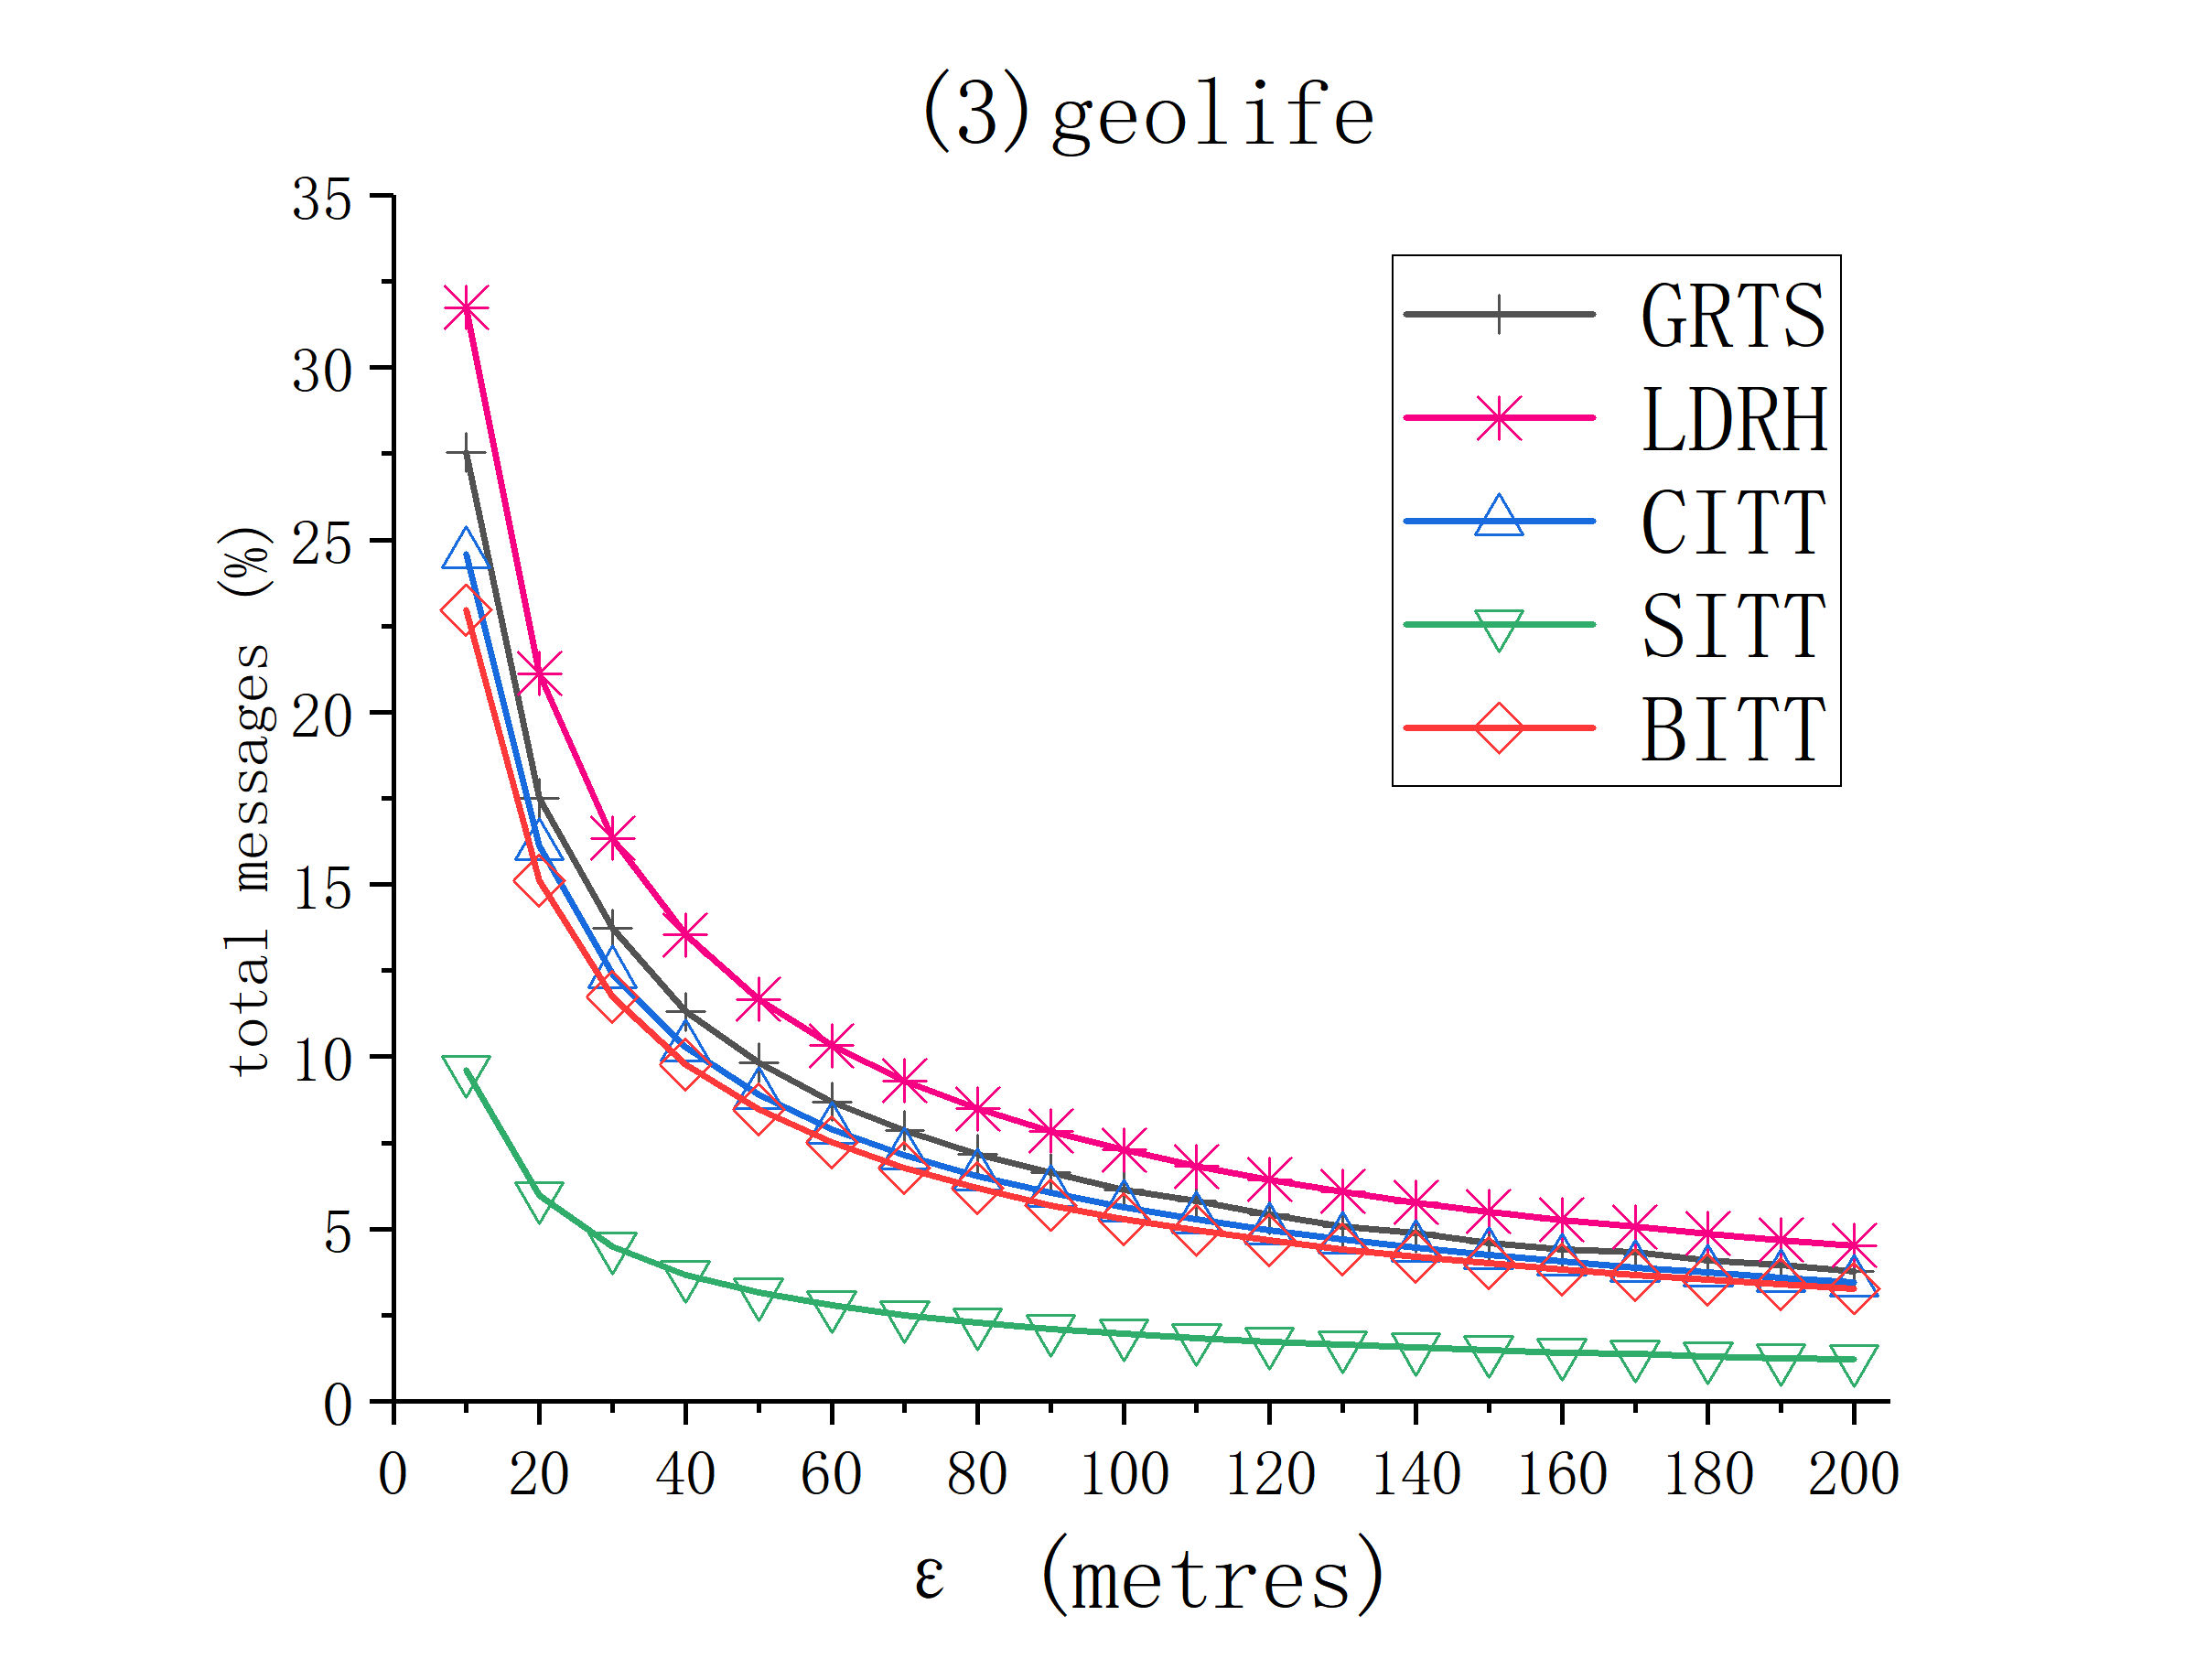
\includegraphics[scale = 0.210]{figures/Fig-geolife-total-messages.png}\hspace{1ex}
	%\vspace{-1ex}
	\caption{\small Evaluation of total messages: varying error bounds $\epsilon_{sed}$ and $\epsilon_{ped}$.}
	\label{fig:total-message}
	%\vspace{-1ex}
\end{figure*}

\begin{figure*}[tb!]
	\centering
	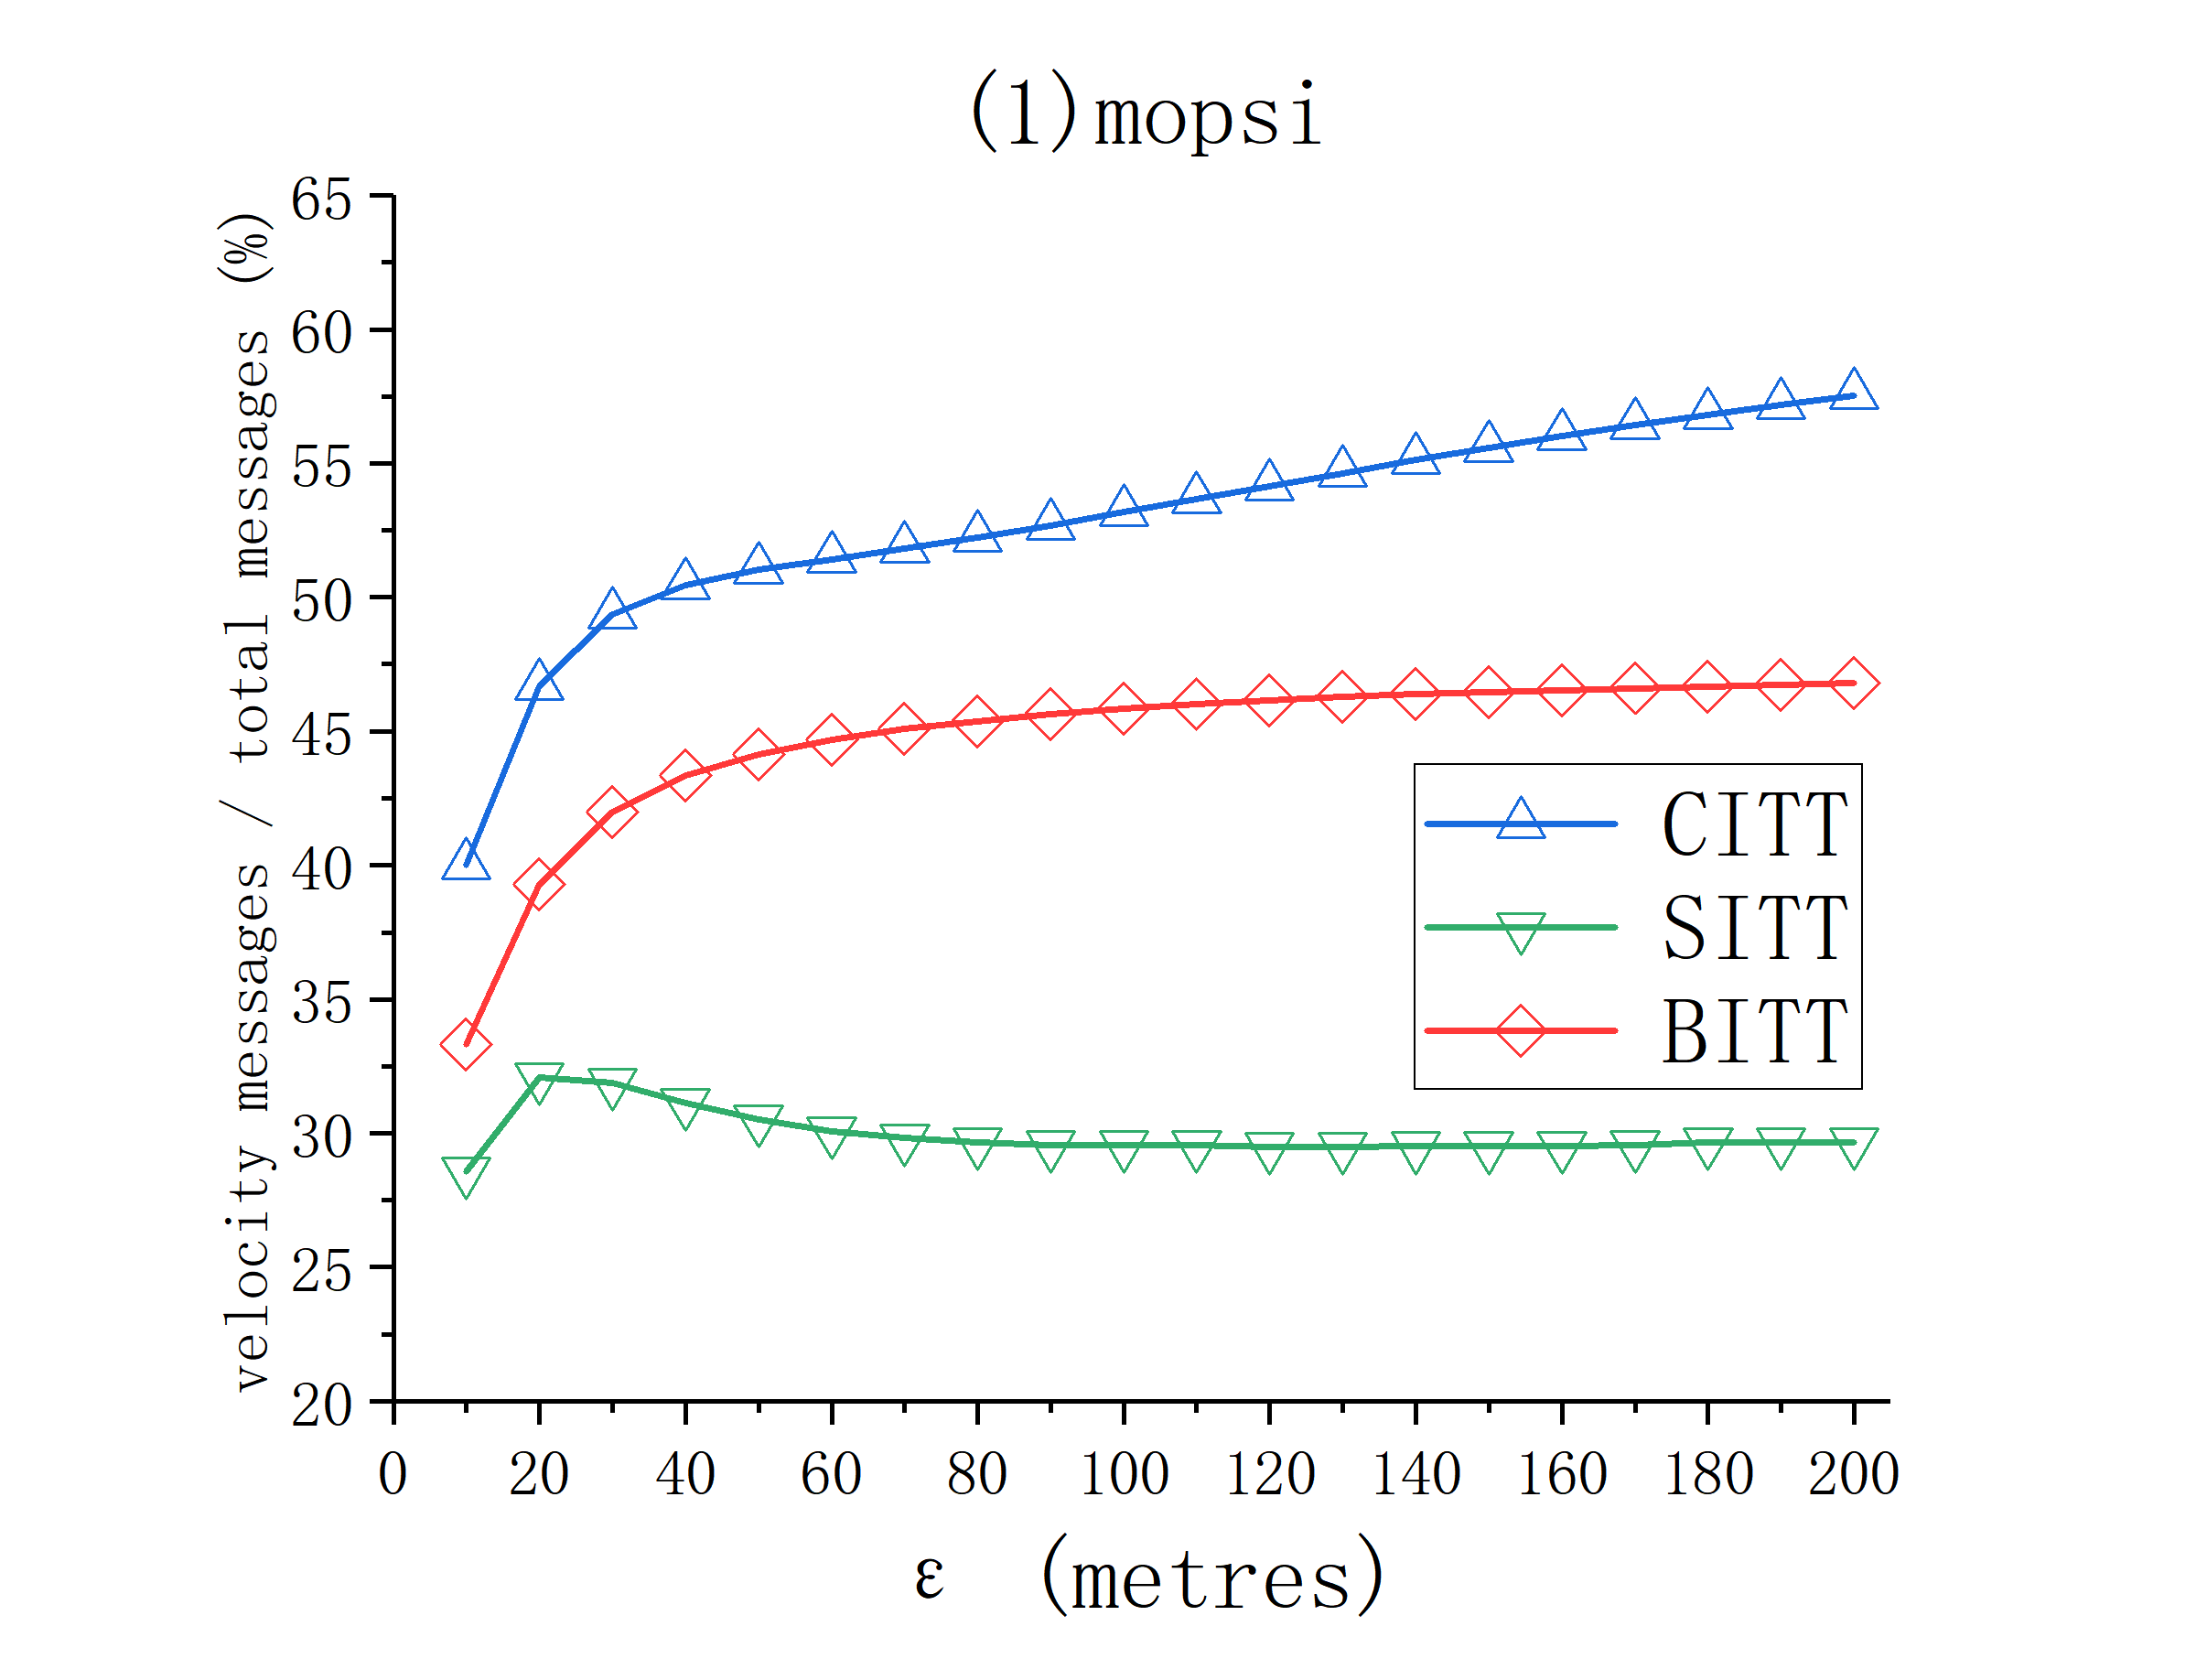
\includegraphics[scale = 0.210]{figures/Fig-mopsi-speed-messages.png}\hspace{1ex}
	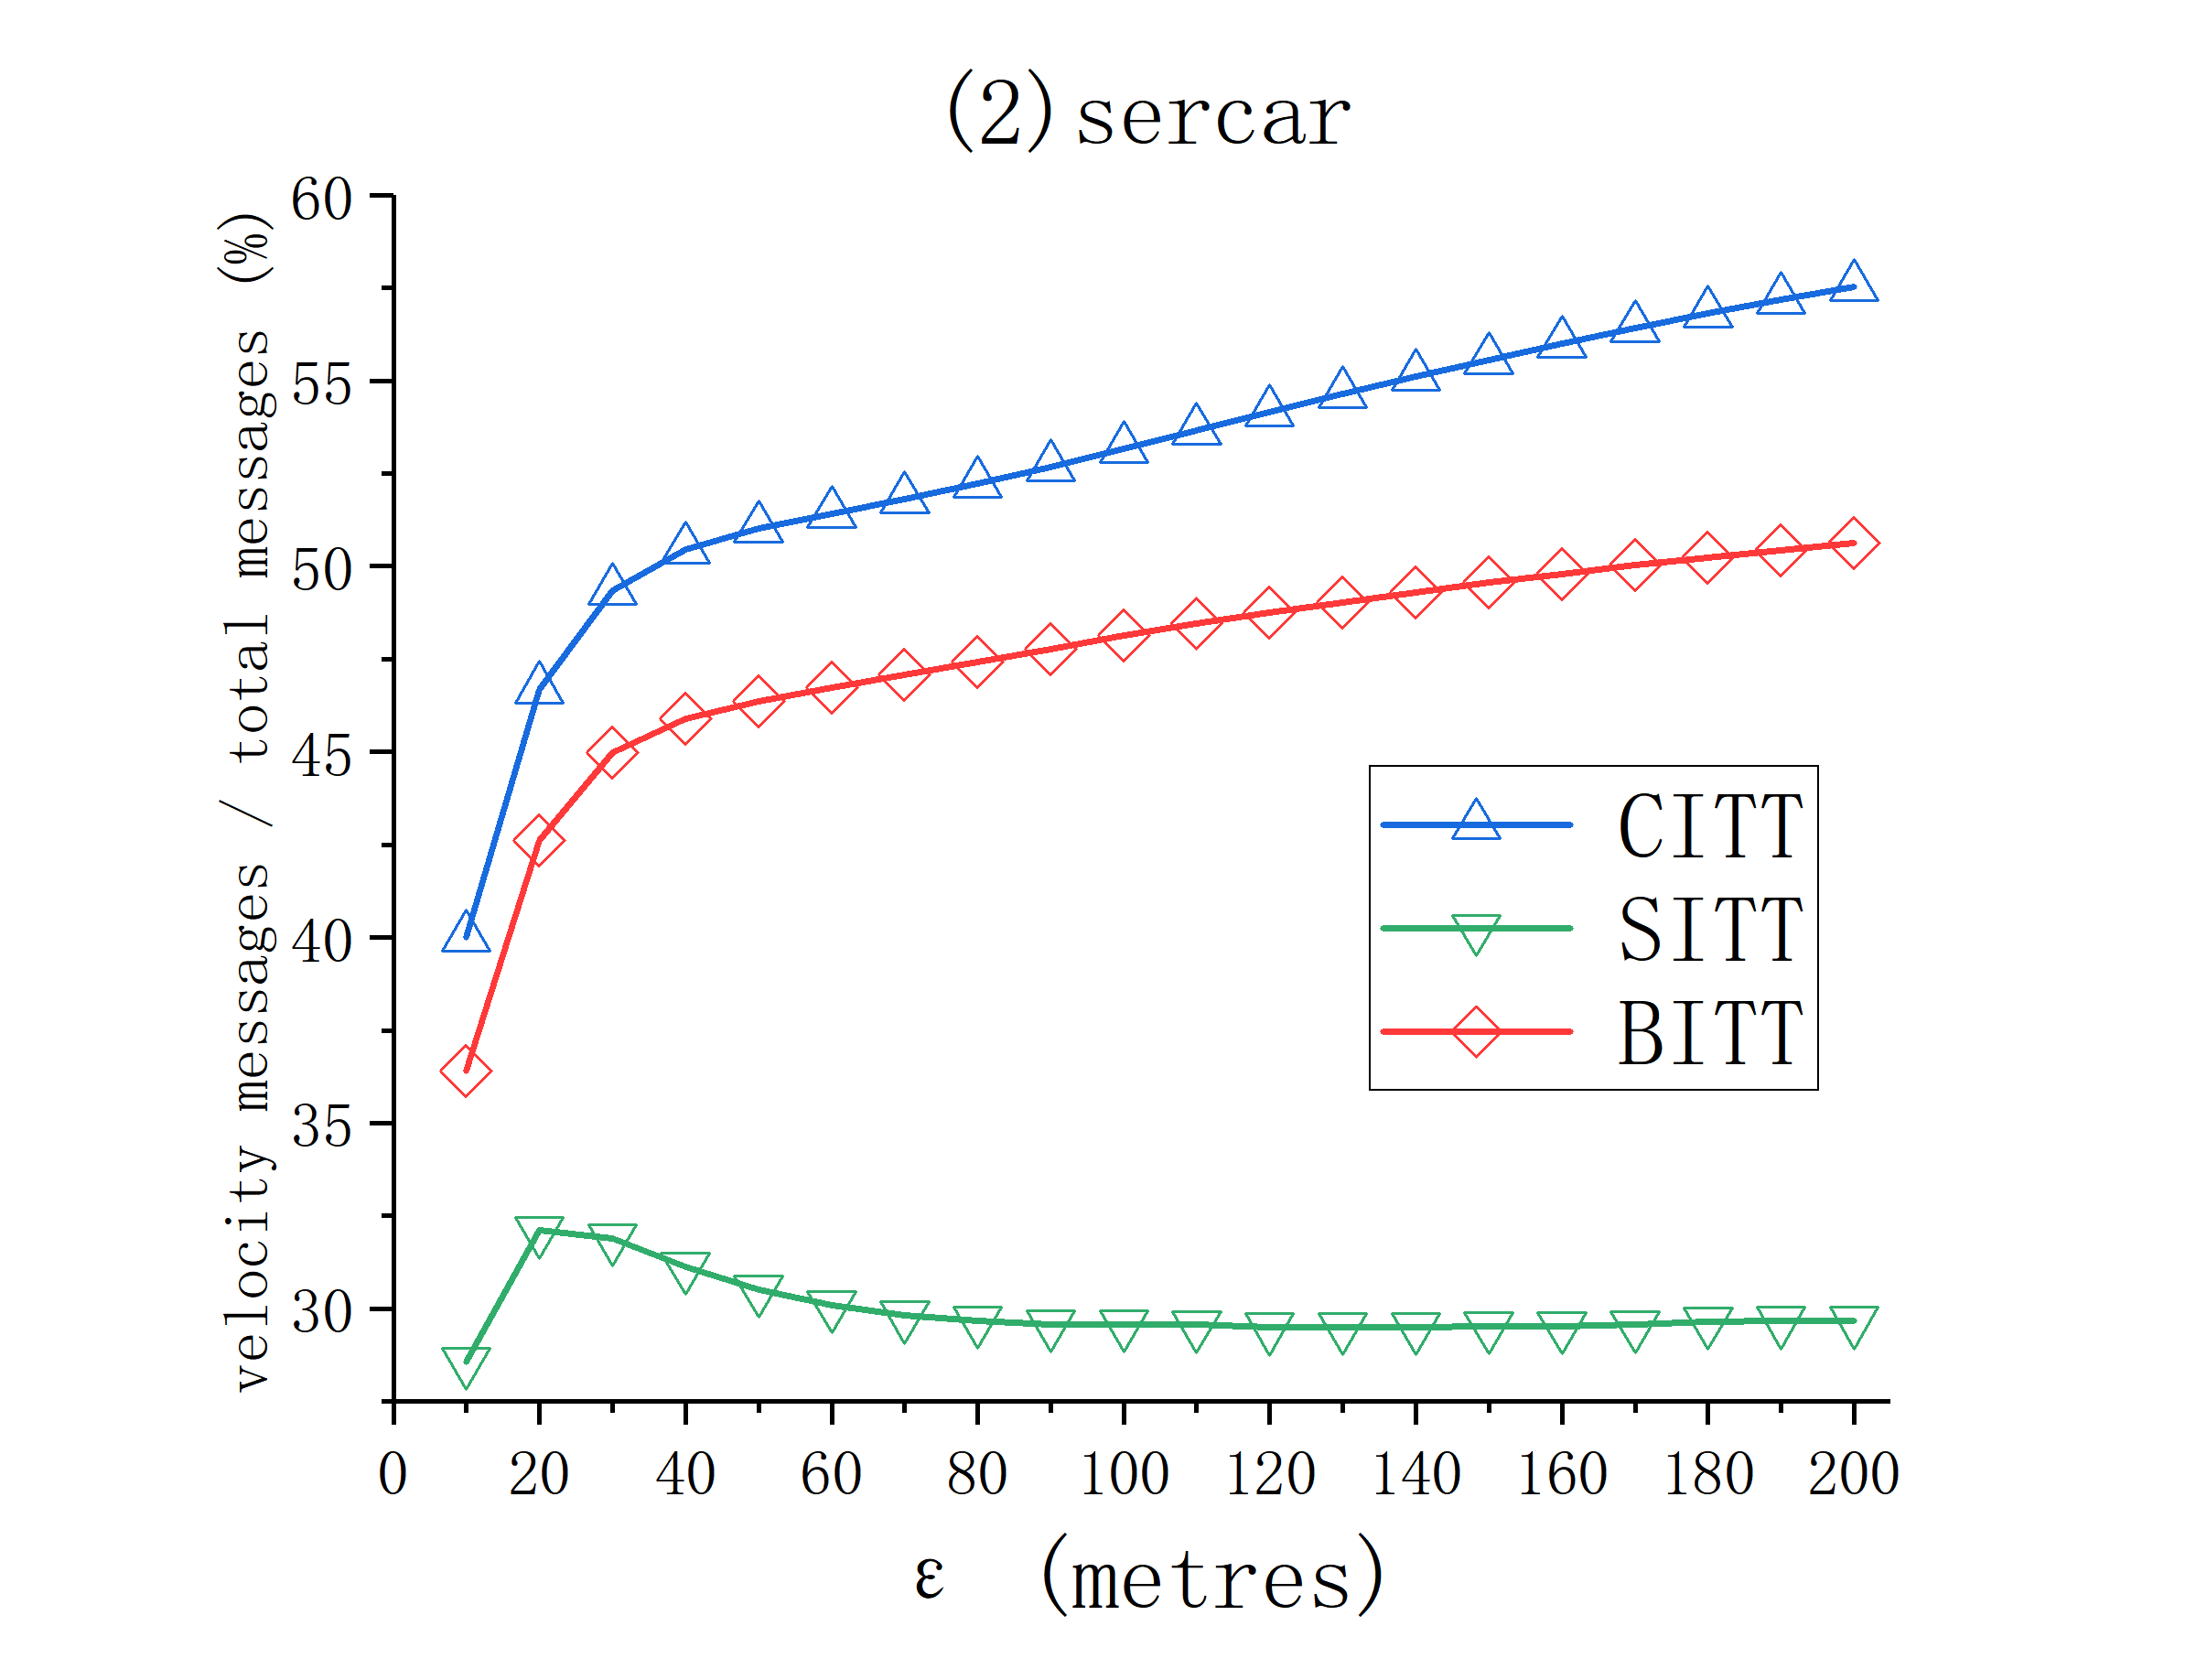
\includegraphics[scale = 0.210]{figures/Fig-sercar-speed-messages.png}\hspace{1ex}
	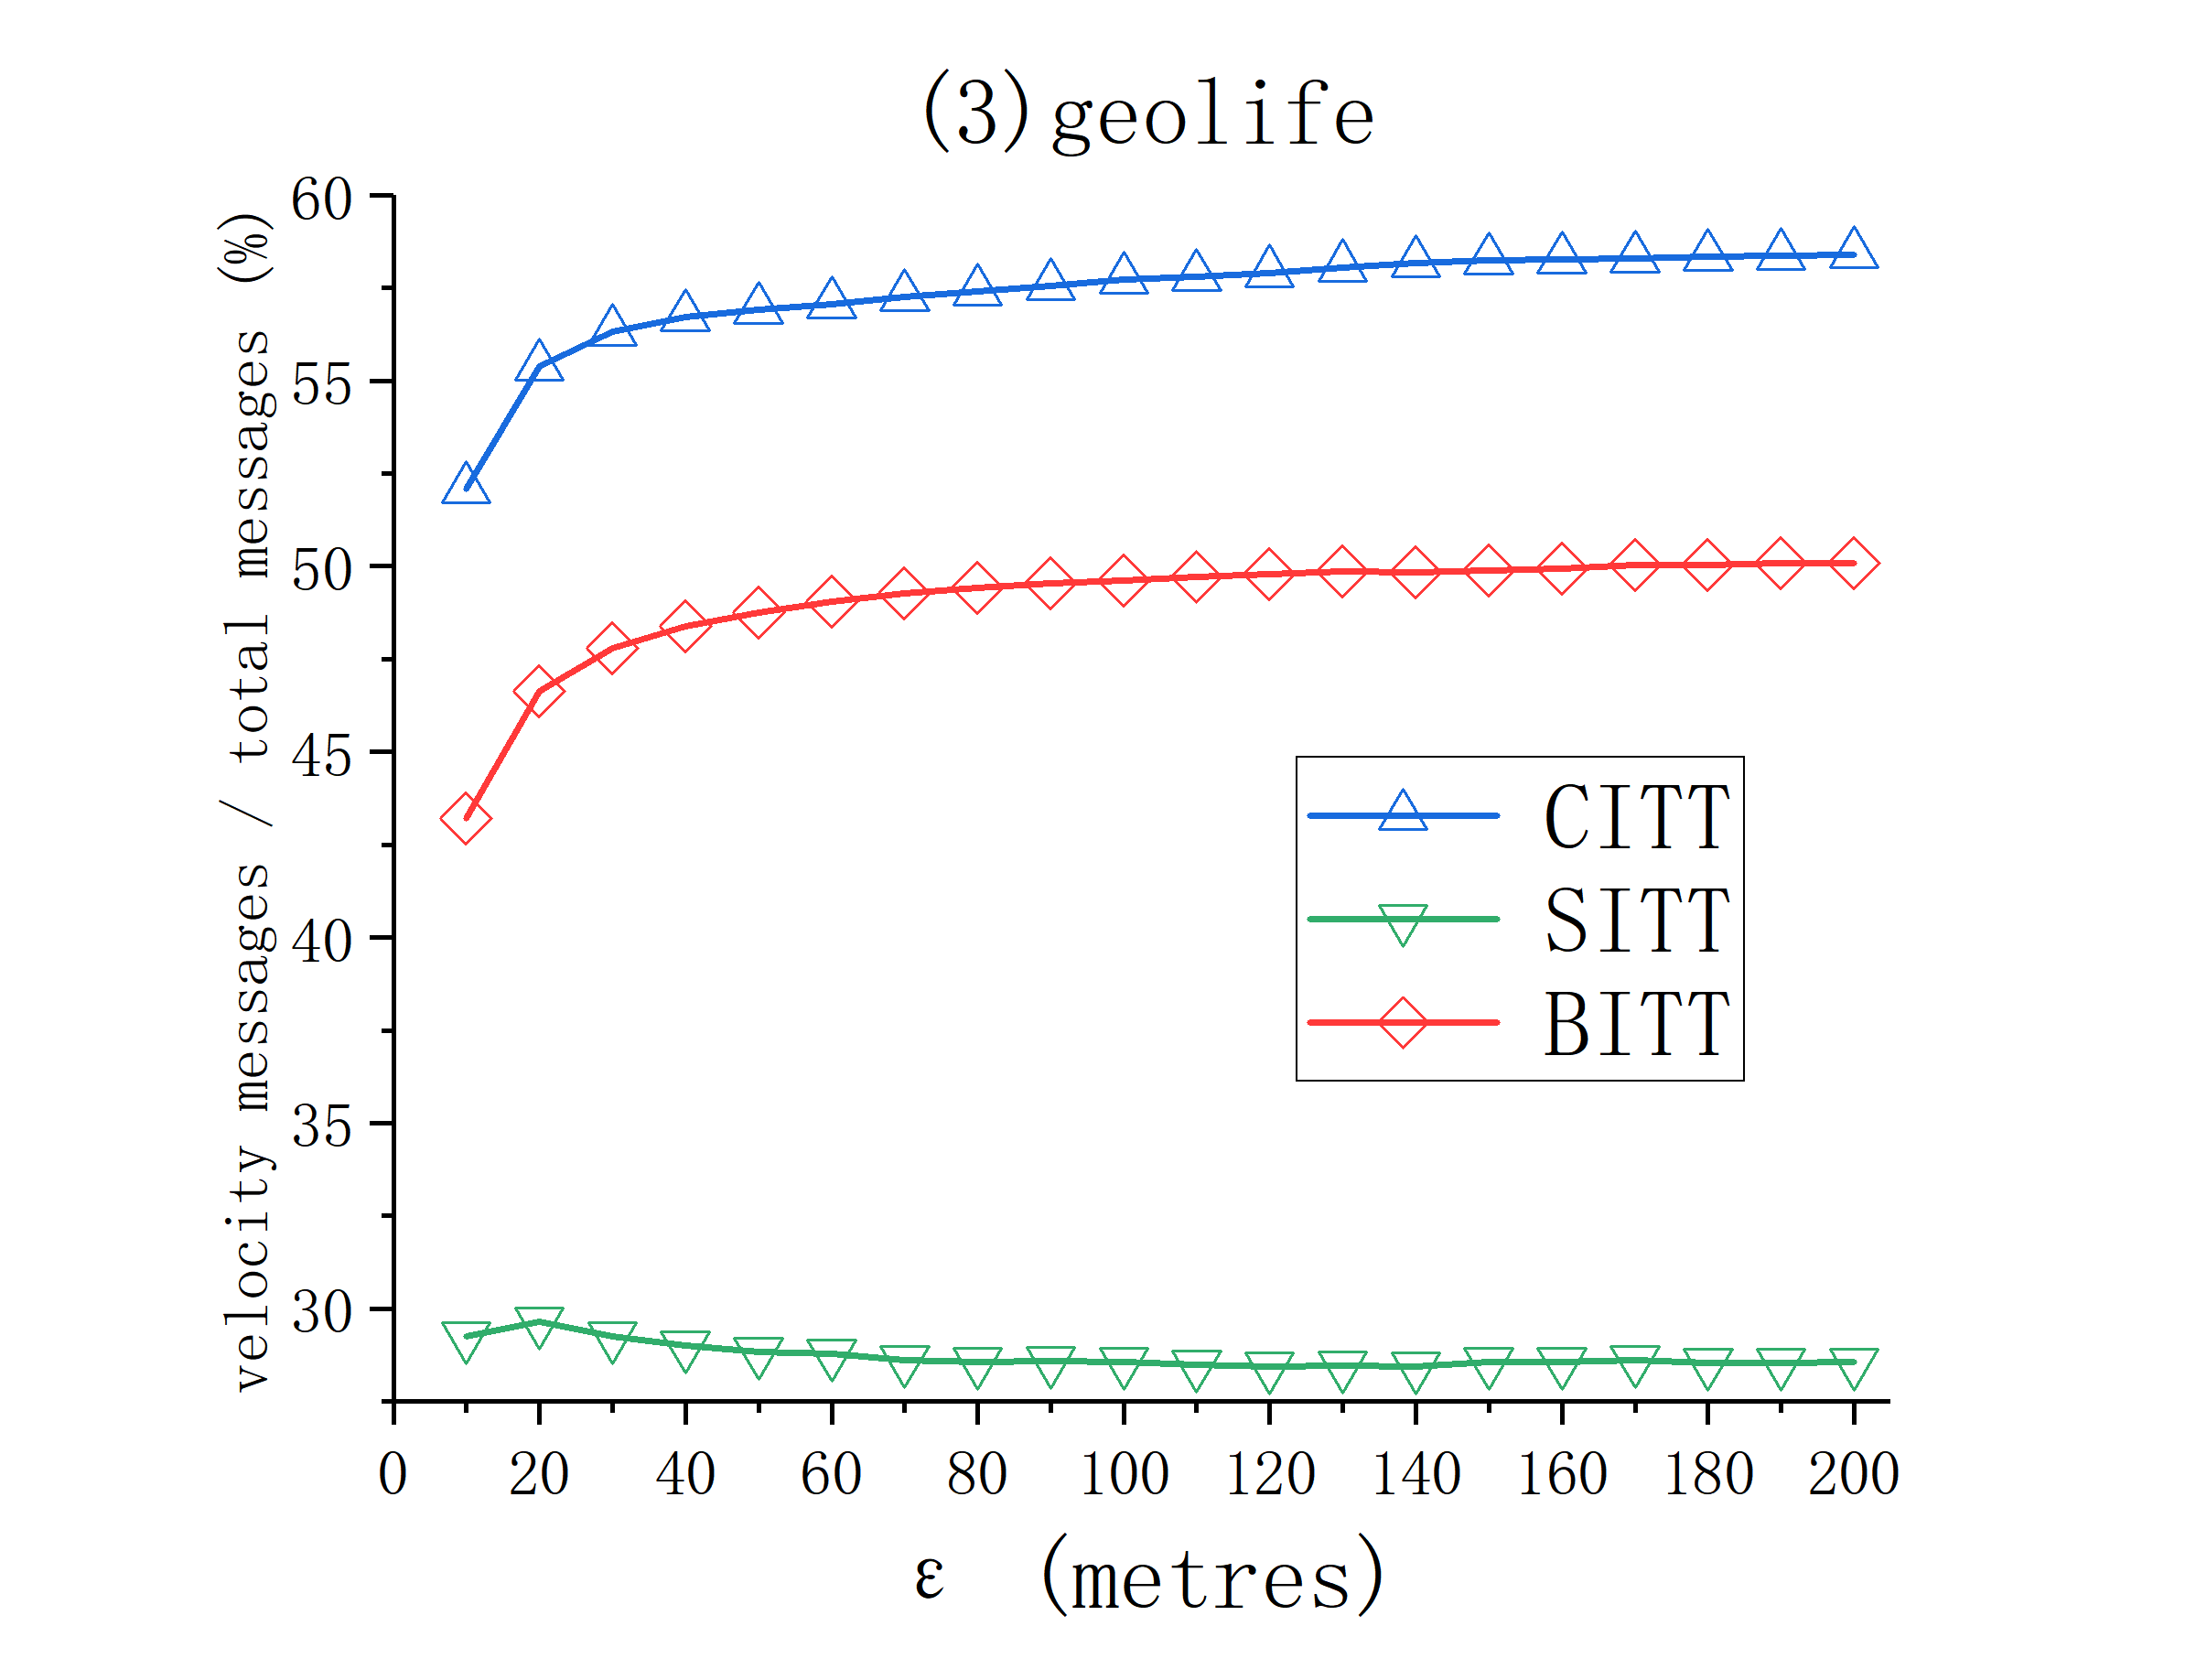
\includegraphics[scale = 0.210]{figures/Fig-geolife-speed-messages.png}\hspace{1ex}
	%\vspace{-1ex}
	\caption{\small Evaluation of velocities messages: varying error bounds $\epsilon_{sed}$ and $\epsilon_{ped}$.}
	\label{fig:speed-message}
	%\vspace{-1ex}
\end{figure*}

\stitle{Messages.}
%To evaluate the impacts of distance metrics and error bounds on messages of \citt, \sitt and \bitt vs. \ldrh and \grts, we varied the error bound (either $\epsilon_{sed}$ or $\epsilon_{ped}$) from $10$ meters to $200$ meters on the entire three datasets, respectively. 

\ni (1) We can see that the amount of transmitted messages in the \ldrh is the largest, and this value is the smallest in \sitt, because the ped threshold is looser than sed.

\ni (2) Since \ldrh updates the position information every time the velocity is updated, the percentage of velocity updates has always been 50\%.

\ni (3) The proportions of velocities updates of \citt, \bitt, and \sitt are all greater than \ldrh, because these algorithms constantly calculate and update the velocity during the tracking process.

\ni (4) \grts has the least velocities update ratio. This is because \grts only updates the velocities messages when the buffer is cleared, and mainly transmits position information.



\begin{figure*}[tb!]
	\centering
	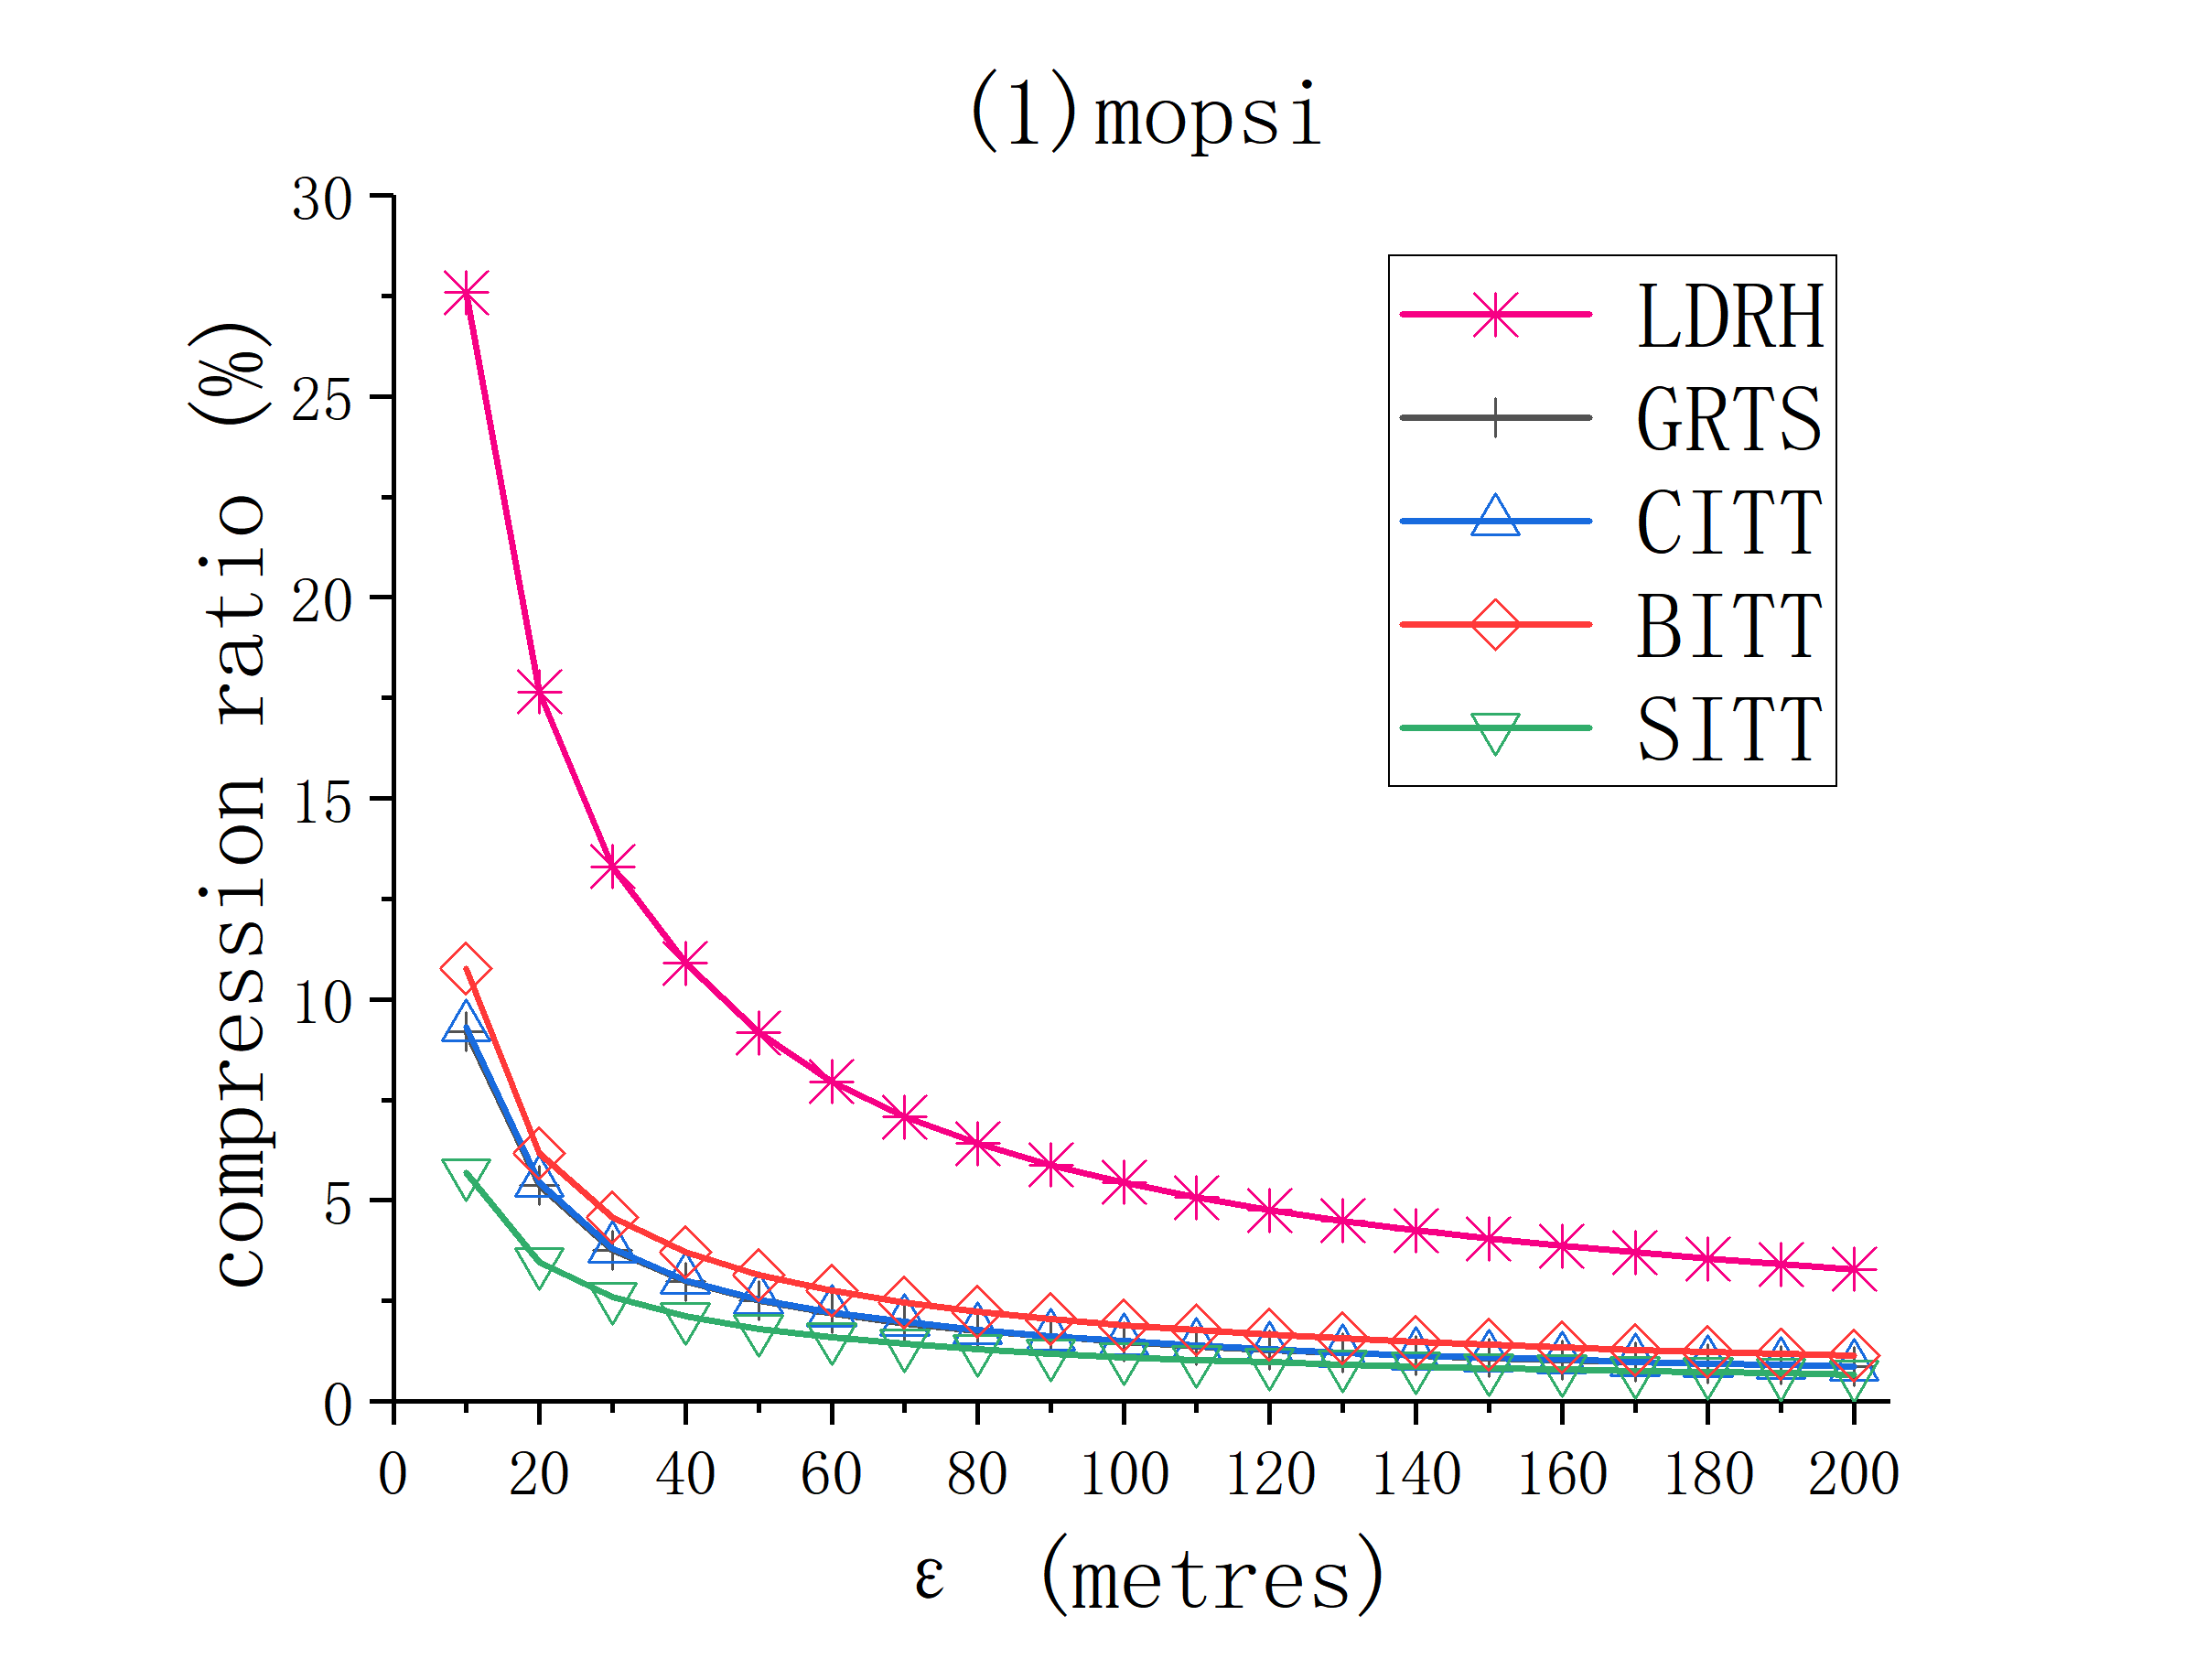
\includegraphics[scale = 0.210]{figures/Fig-mopsi-compression-ratio.png}\hspace{1ex}
	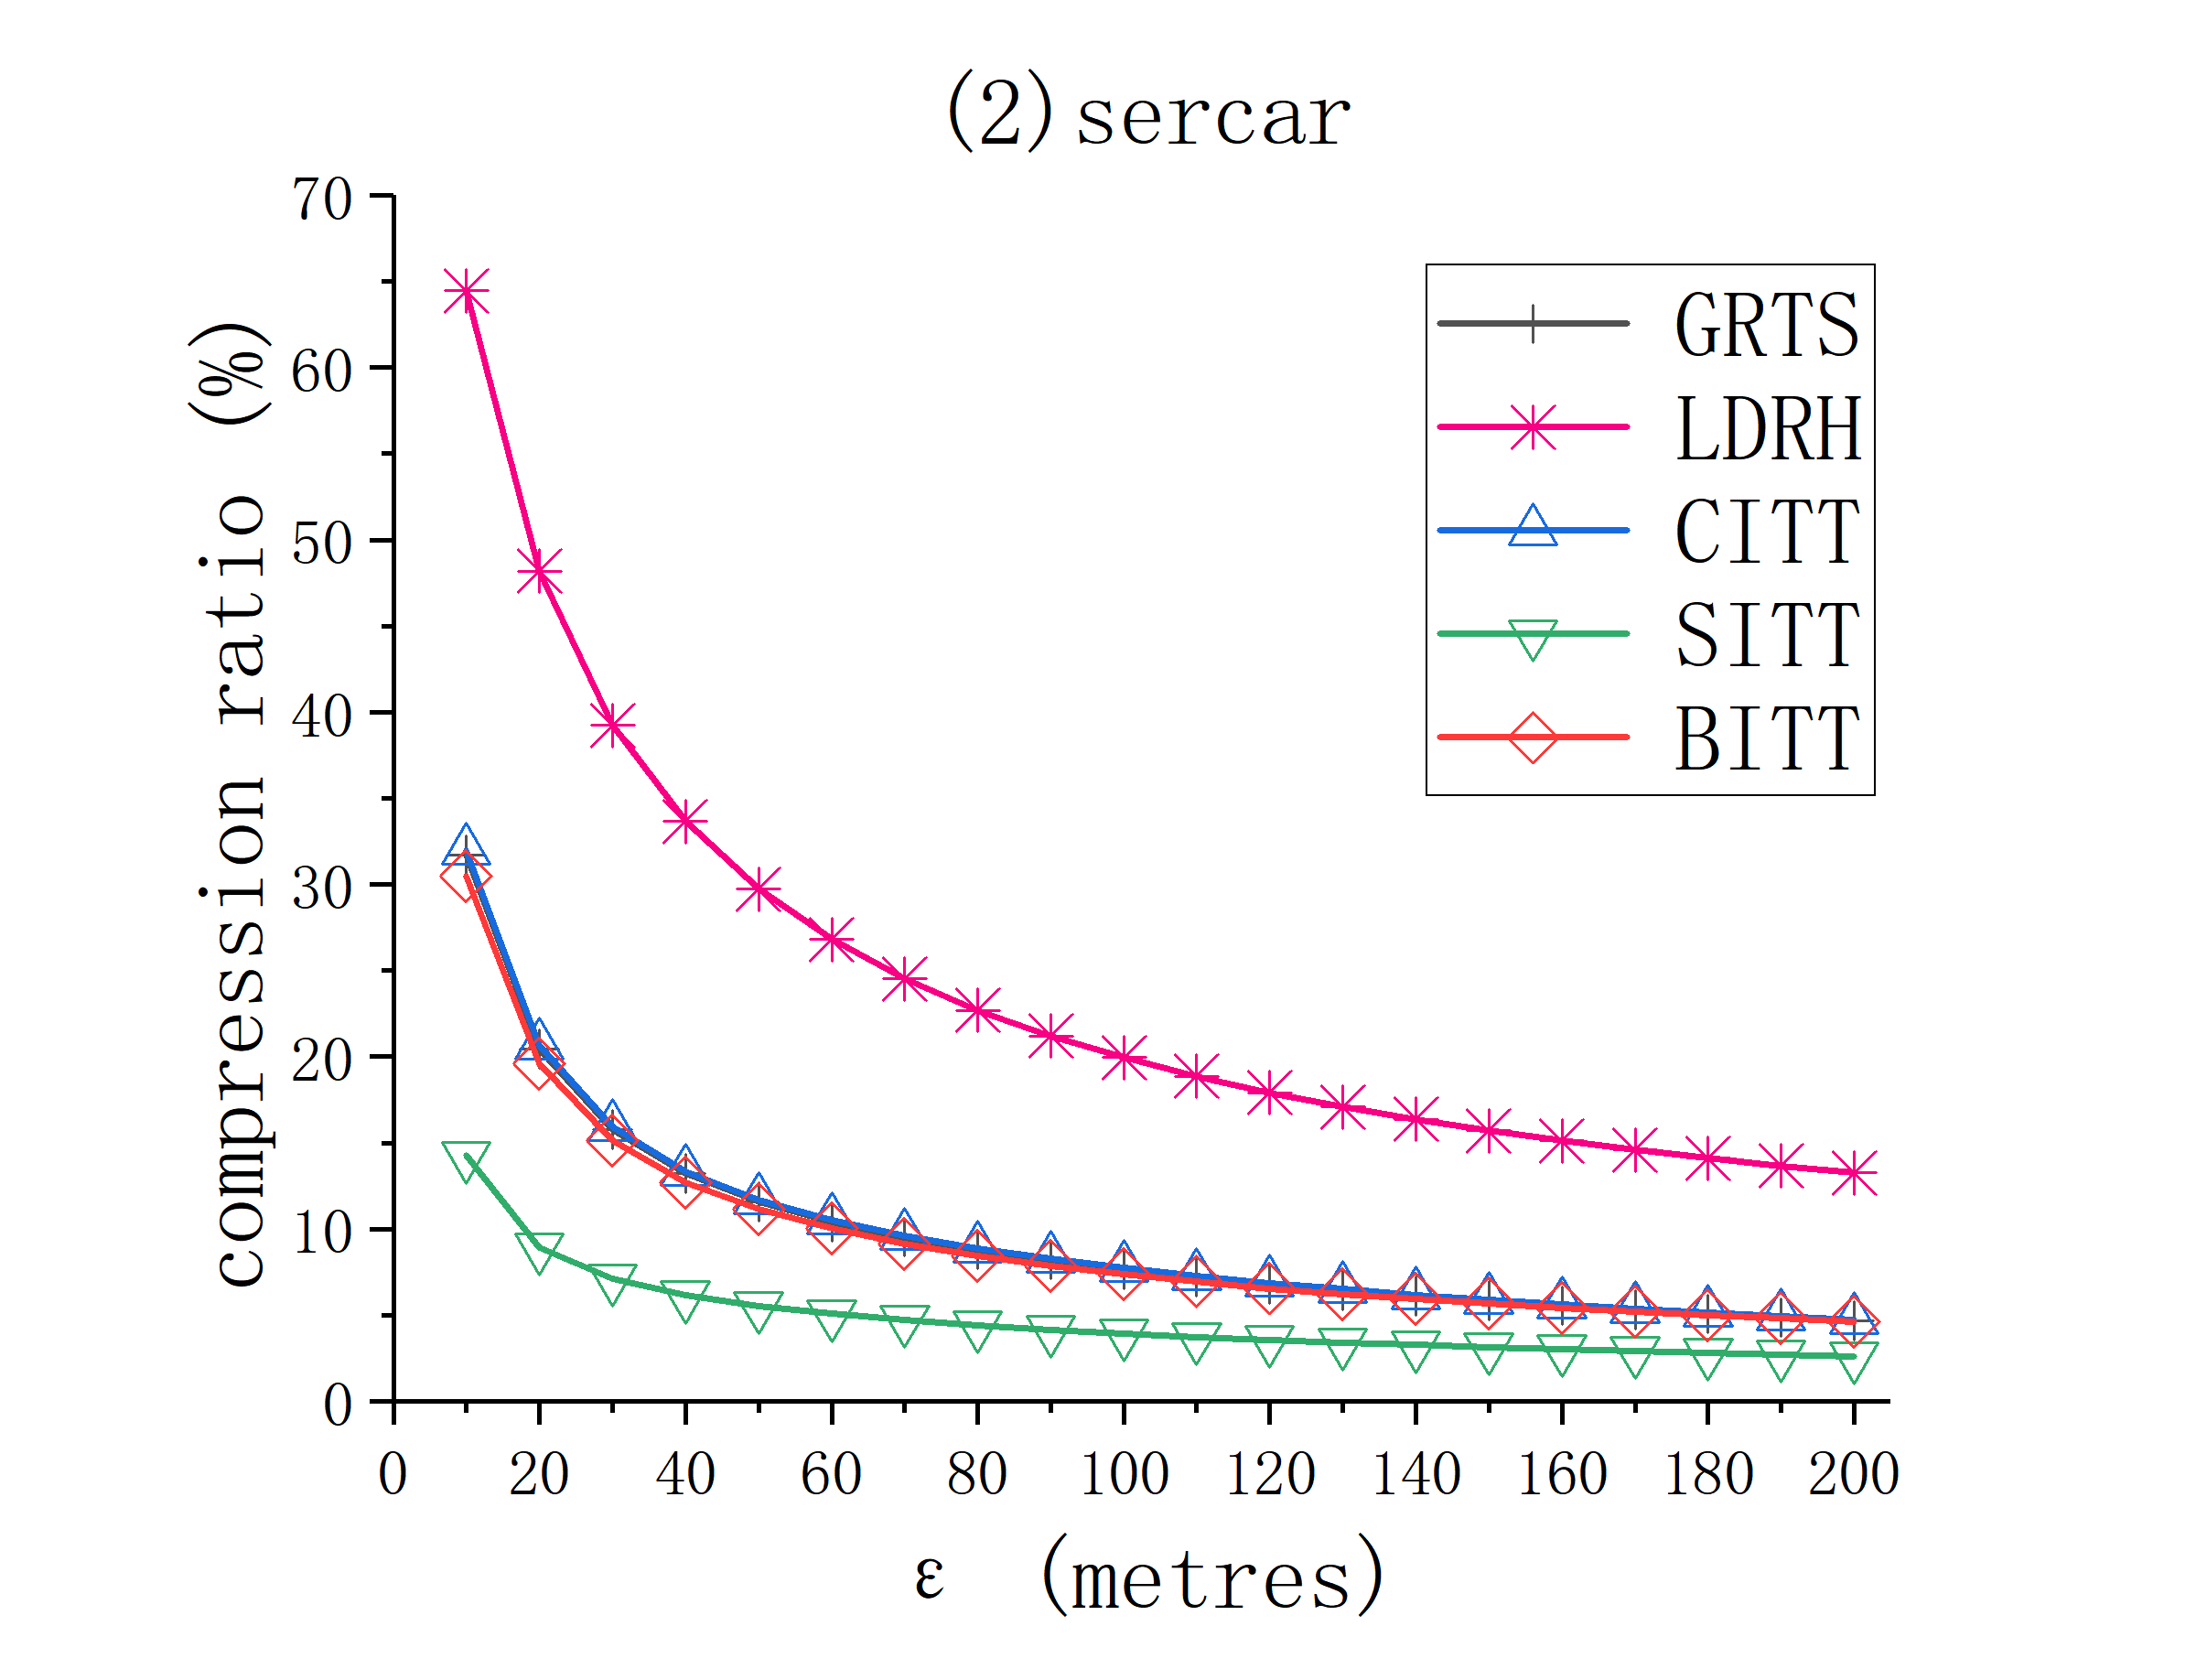
\includegraphics[scale = 0.210]{figures/Fig-sercar-compression-ratio.png}\hspace{1ex}
	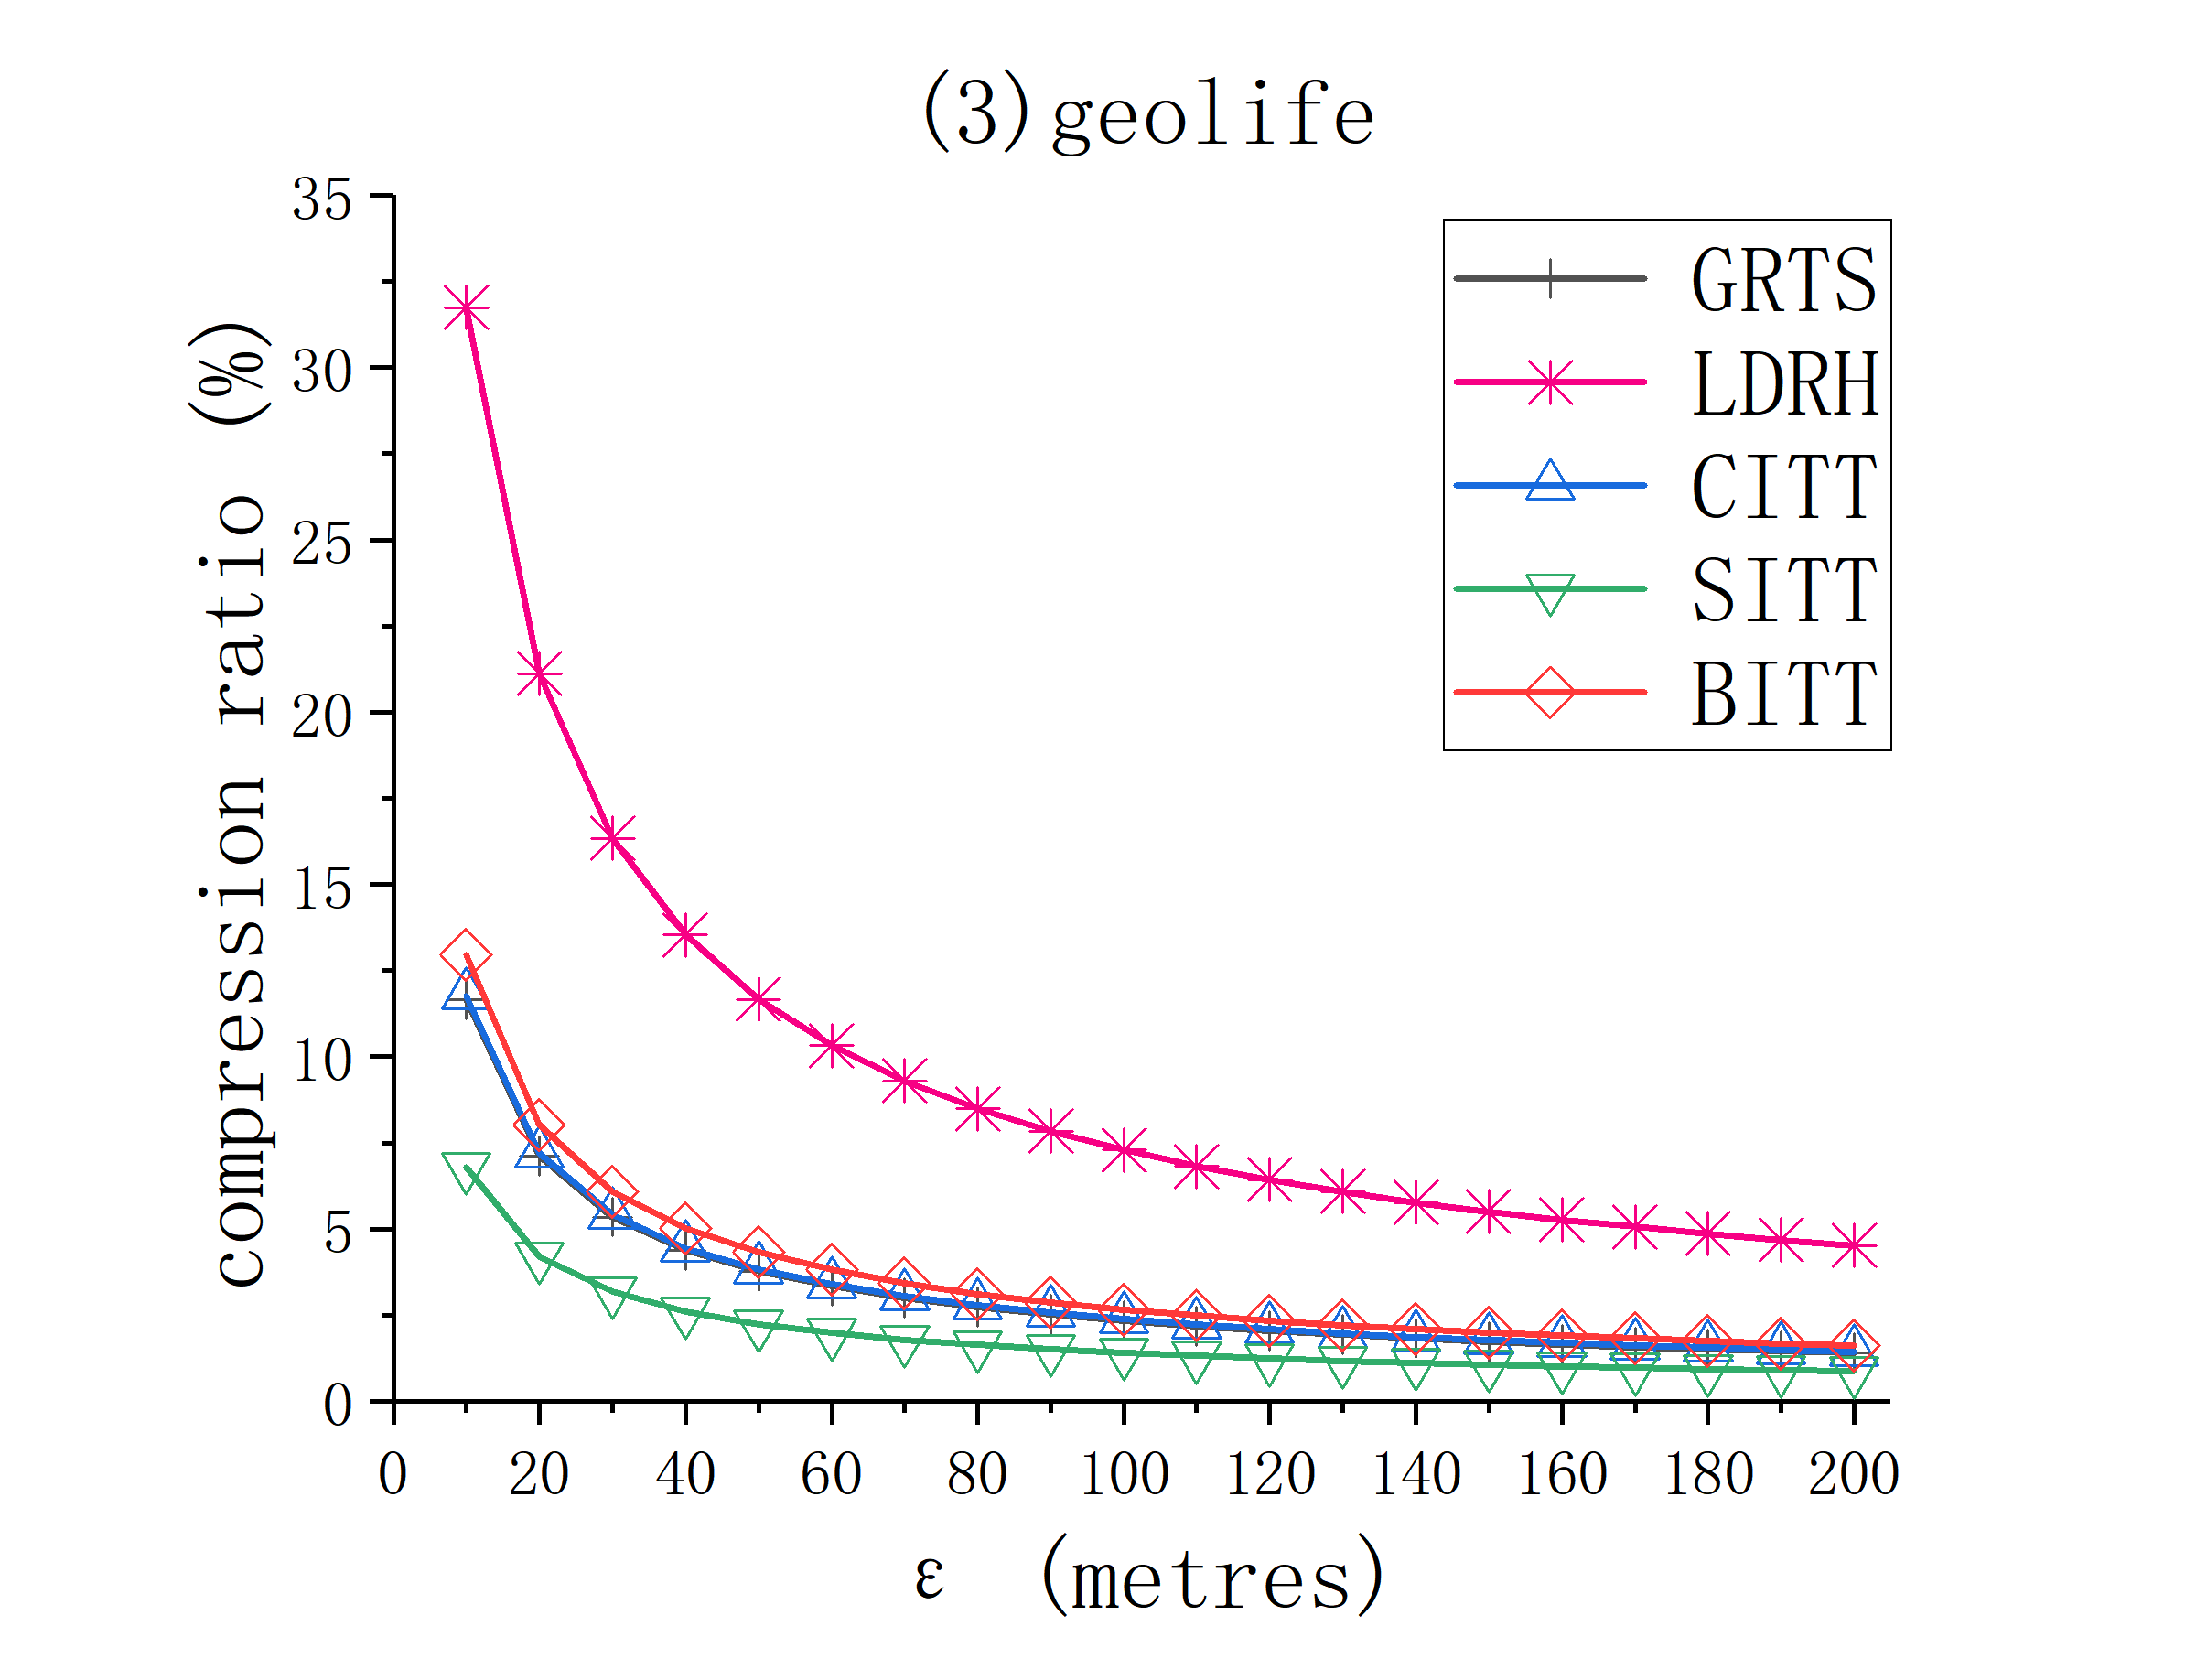
\includegraphics[scale = 0.210]{figures/Fig-geolife-compression-ratio.png}\hspace{1ex}
	%\vspace{-1ex}
	\caption{\small Evaluation of compression ratio: varying error bounds $\epsilon_{sed}$ and $\epsilon_{ped}$.}
	\label{fig:compression-ratio}
	%\vspace{-1ex}
\end{figure*}


\stitle{Compression ratios.}
\ni (1) When increasing $\epsilon_{sed}$ and $\epsilon_{ped}$, the compression ratios of all these algorithms decrease on all datasets.

\ni (2) Algorithm \citt is better than \ldrh {and comparable} with \grts on all datasets and for all $\epsilon$.
The compression ratios of \citt are on average {($29.0\%$, $40.4\%$, $33.5\%$) and ($101.0\%$, $100.9\%$, $101.6\%$)} of \ldrh and
\grts on {datasets (\mopsi, \sercar, \geolife)}, respectively.
For example, when $\epsilon$ = $40$ meters, the compression ratios of algorithms
\ldrh, \citt and \grts are
{($10.9\%$, $33.7\%$, $13.6\%$), ($3.0\%$, $13.3\%$, $4.5\%$) and ($3.0\%$, $13.2\%$, $4.4\%$)} on  {datasets (\mopsi, \sercar, \geolife)}, respectively.

\ni (3) Algorithm \sitt has better compression ratios than \ldrh, \citt and \grts on all datasets and for all $\epsilon$.
The compression ratios of \sitt are on average ($20.0\%$, $69.2\%$, $69.9\%$), ($19.6\%$, $48.4\%$, $48.9\%$) and {($19.7\%$, $58.7\%$, $59.6\%$) of algorithms
	\ldrh, \citt and \grts on {datasets (\mopsi, \sercar, \geolife)}, respectively.
	For example, when $\epsilon$ = $40$ meters, the compression ratios of algorithm
	\sitt are ($2.1\%$, $6.1\%$, $2.6\%$) on datasets (\mopsi, \sercar, \geolife), respectively.
	
	\ni (4) The compression ratios of algorithm \bitt are between \citt and \sitt.







\begin{figure*}[tb!]
	\centering
	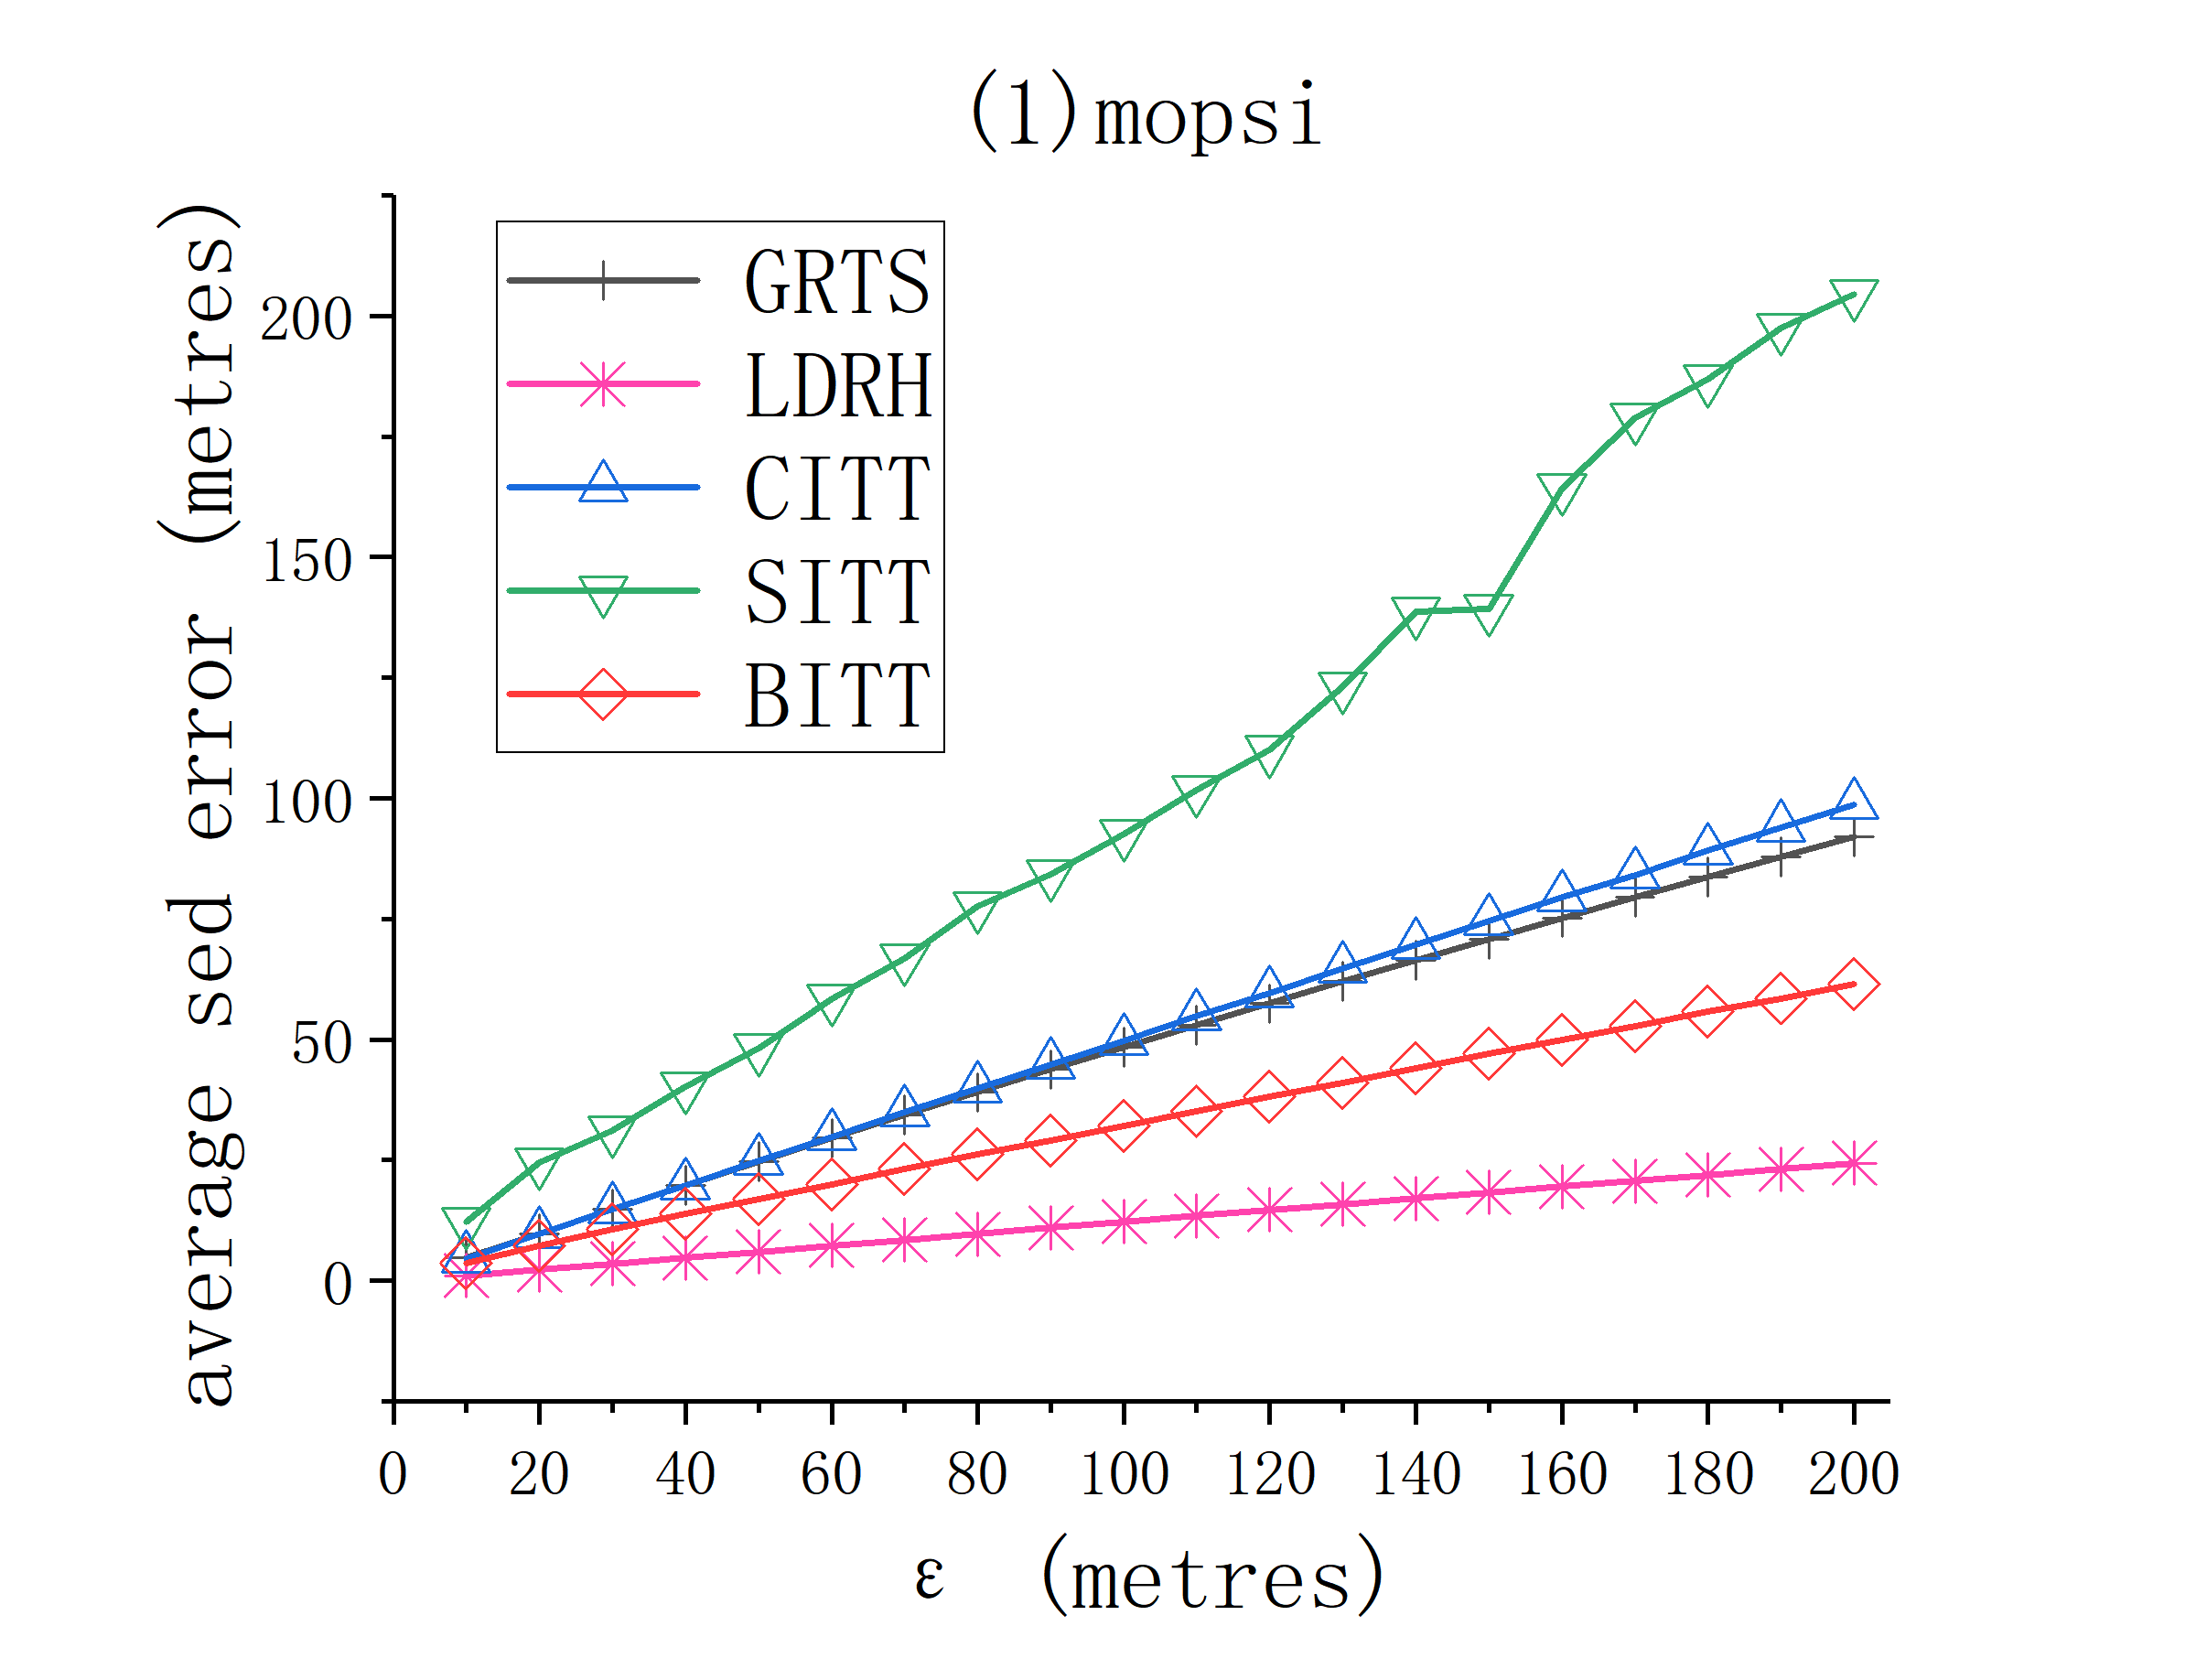
\includegraphics[scale = 0.210]{figures/Fig-mopsi-sed-error.png}\hspace{1ex}
	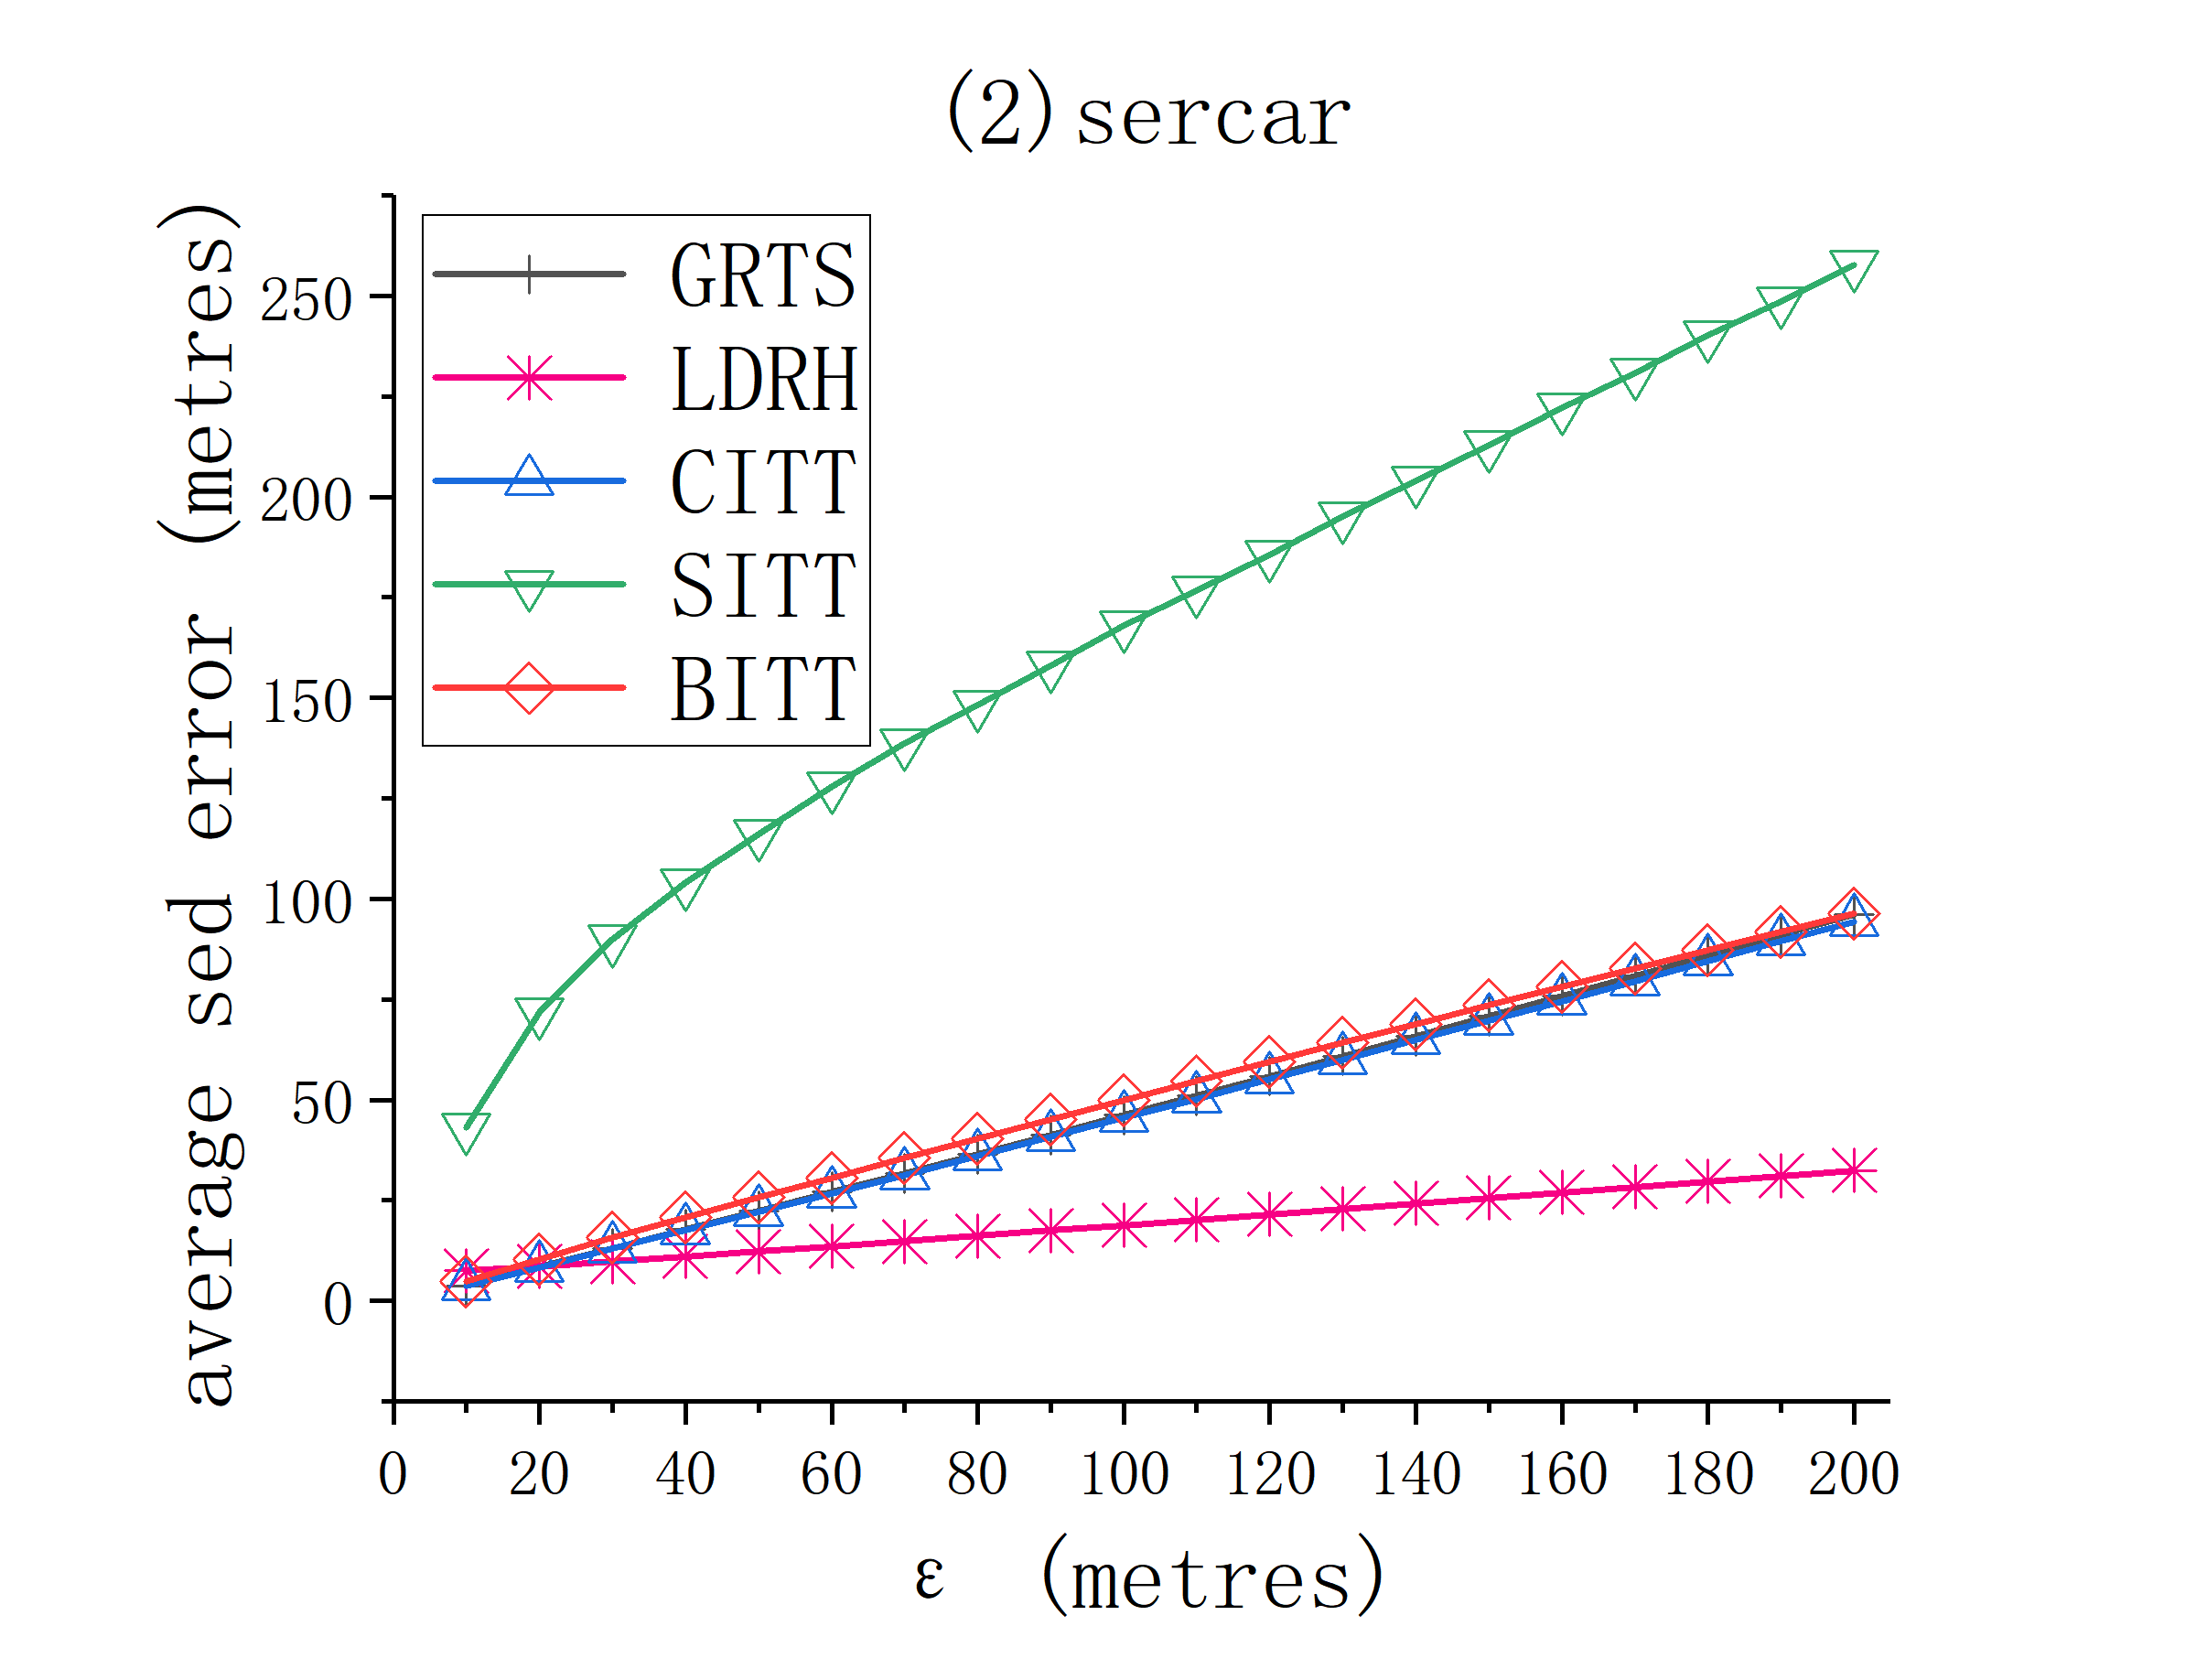
\includegraphics[scale = 0.210]{figures/Fig-sercar-sed-error.png}\hspace{1ex}
	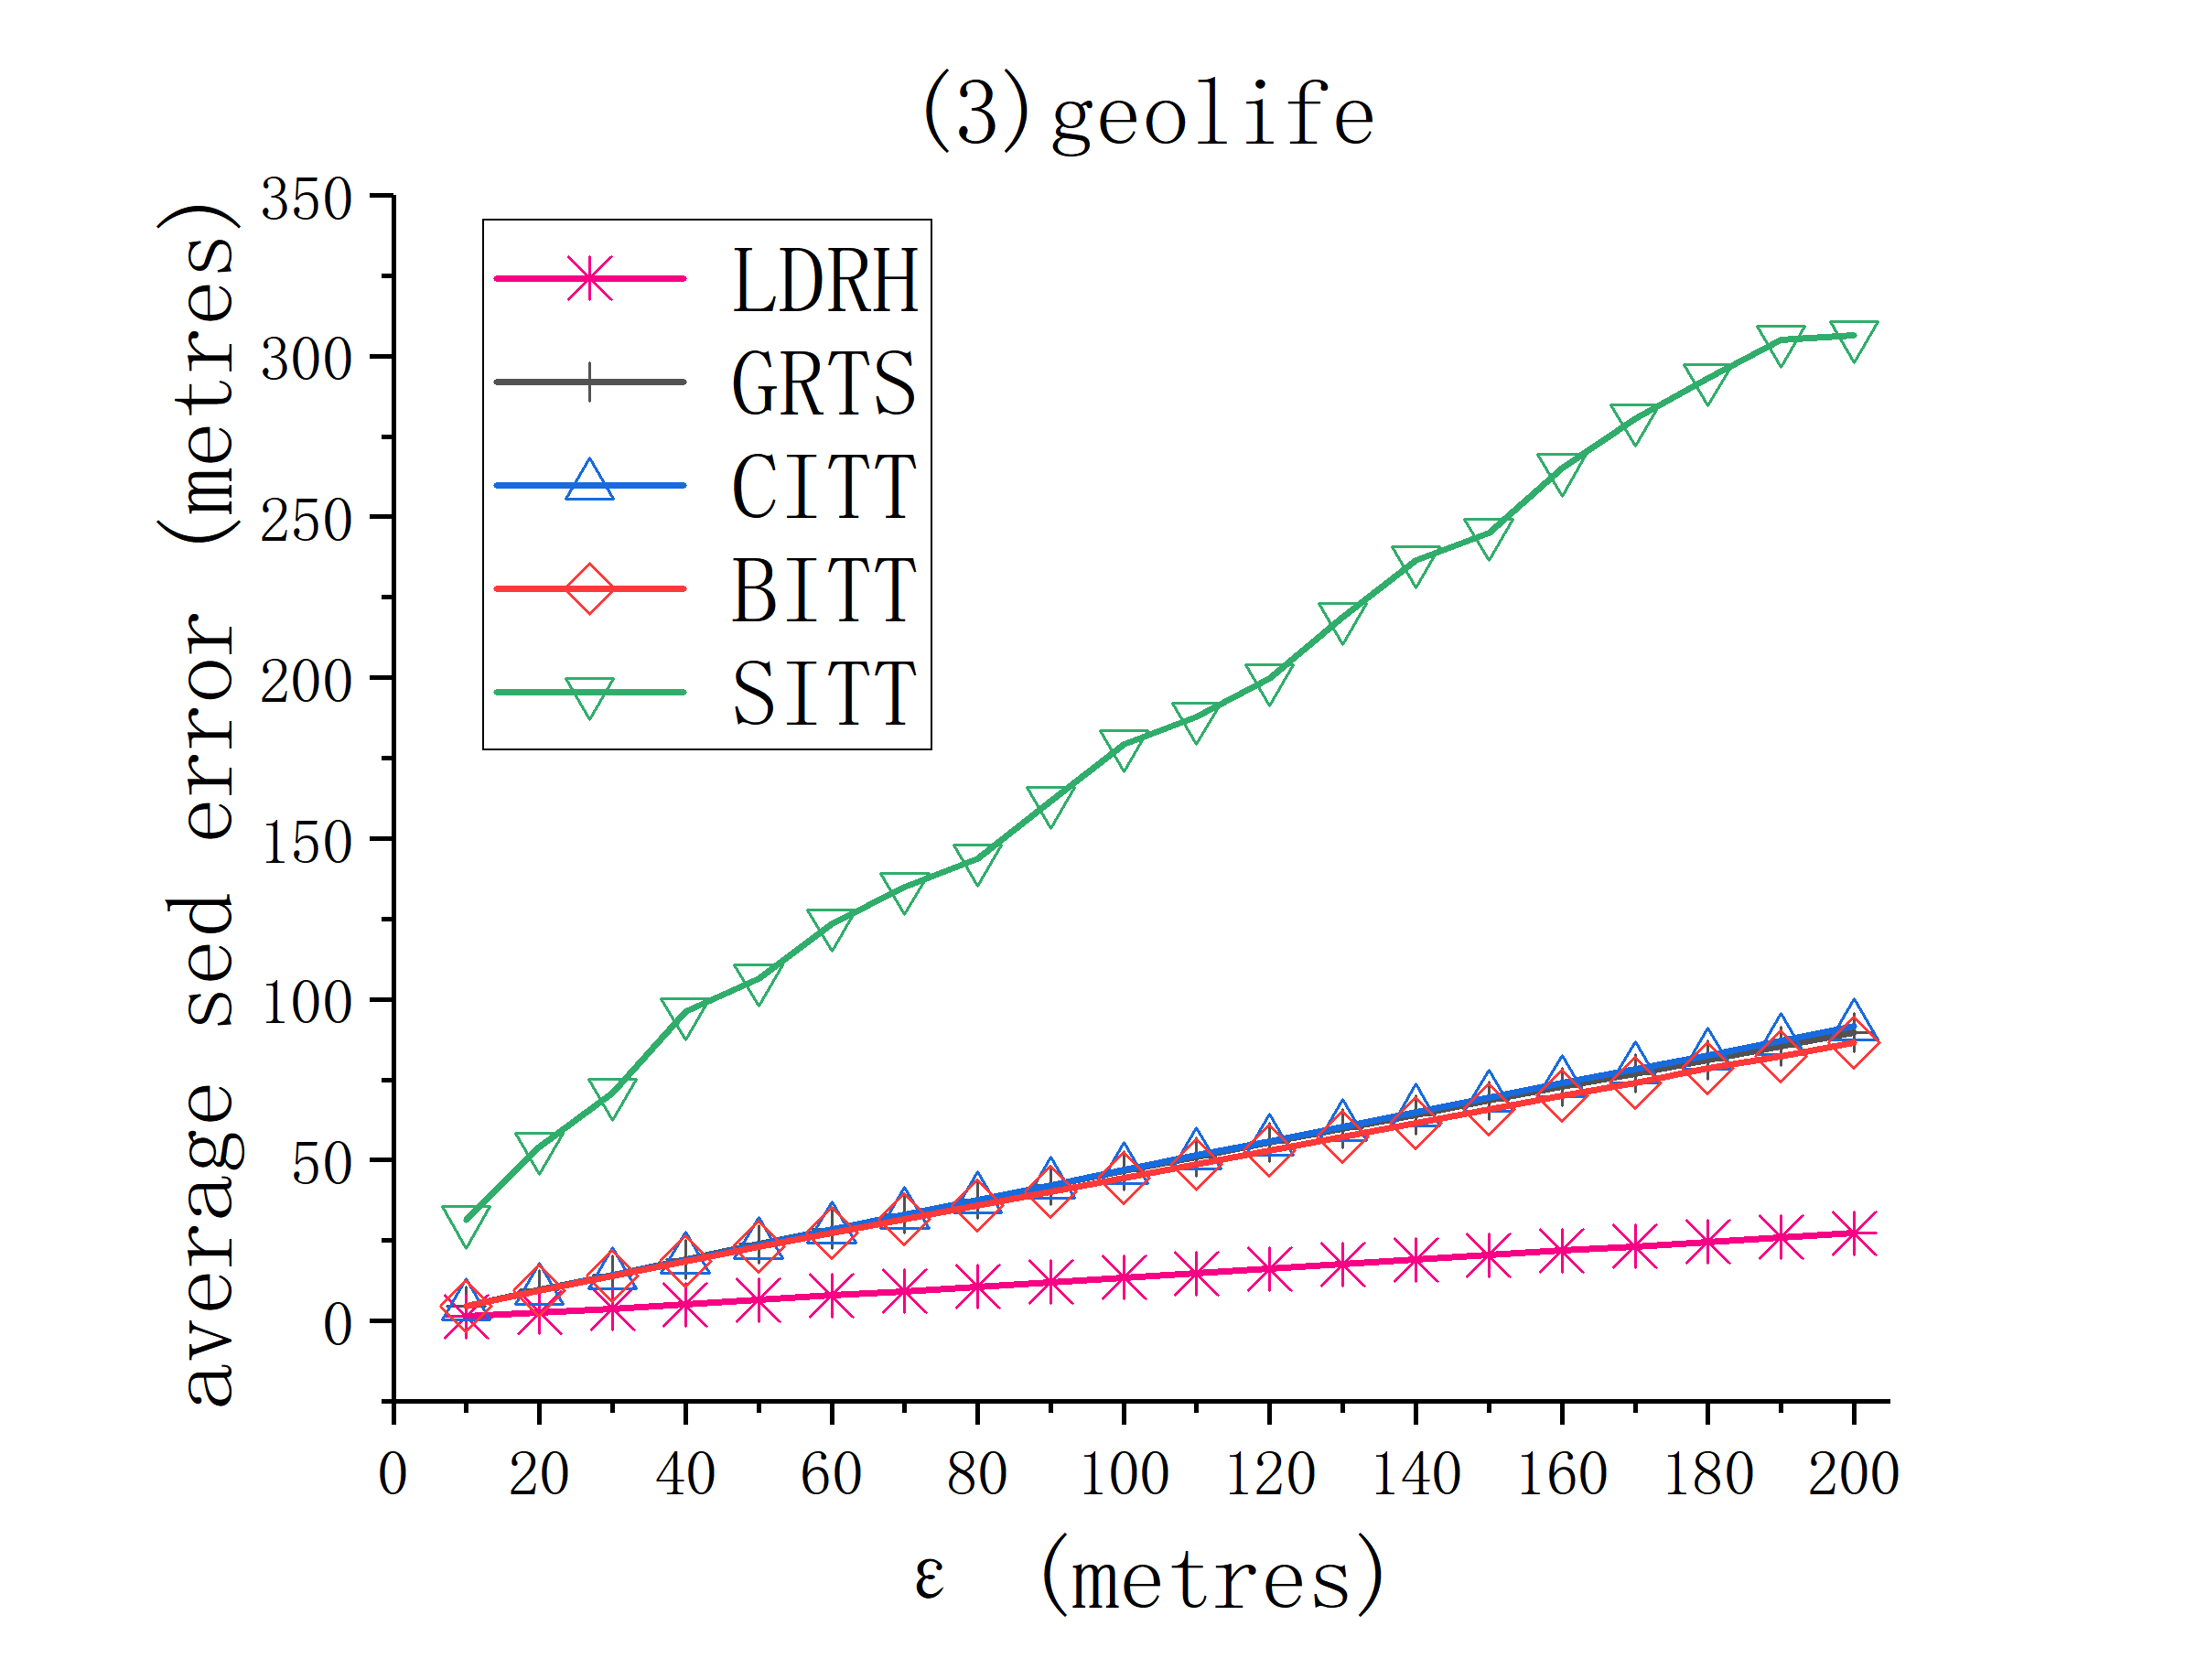
\includegraphics[scale = 0.210]{figures/Fig-geolife-sed-error.png}\hspace{1ex}
	%\vspace{-1ex}
	\caption{\small Evaluation of sed error: varying error bounds $\epsilon_{sed}$ and $\epsilon_{ped}$.}
	\label{fig:sed-error}
	%\vspace{-1ex}
\end{figure*}

\begin{figure*}[tb!]
	\centering
	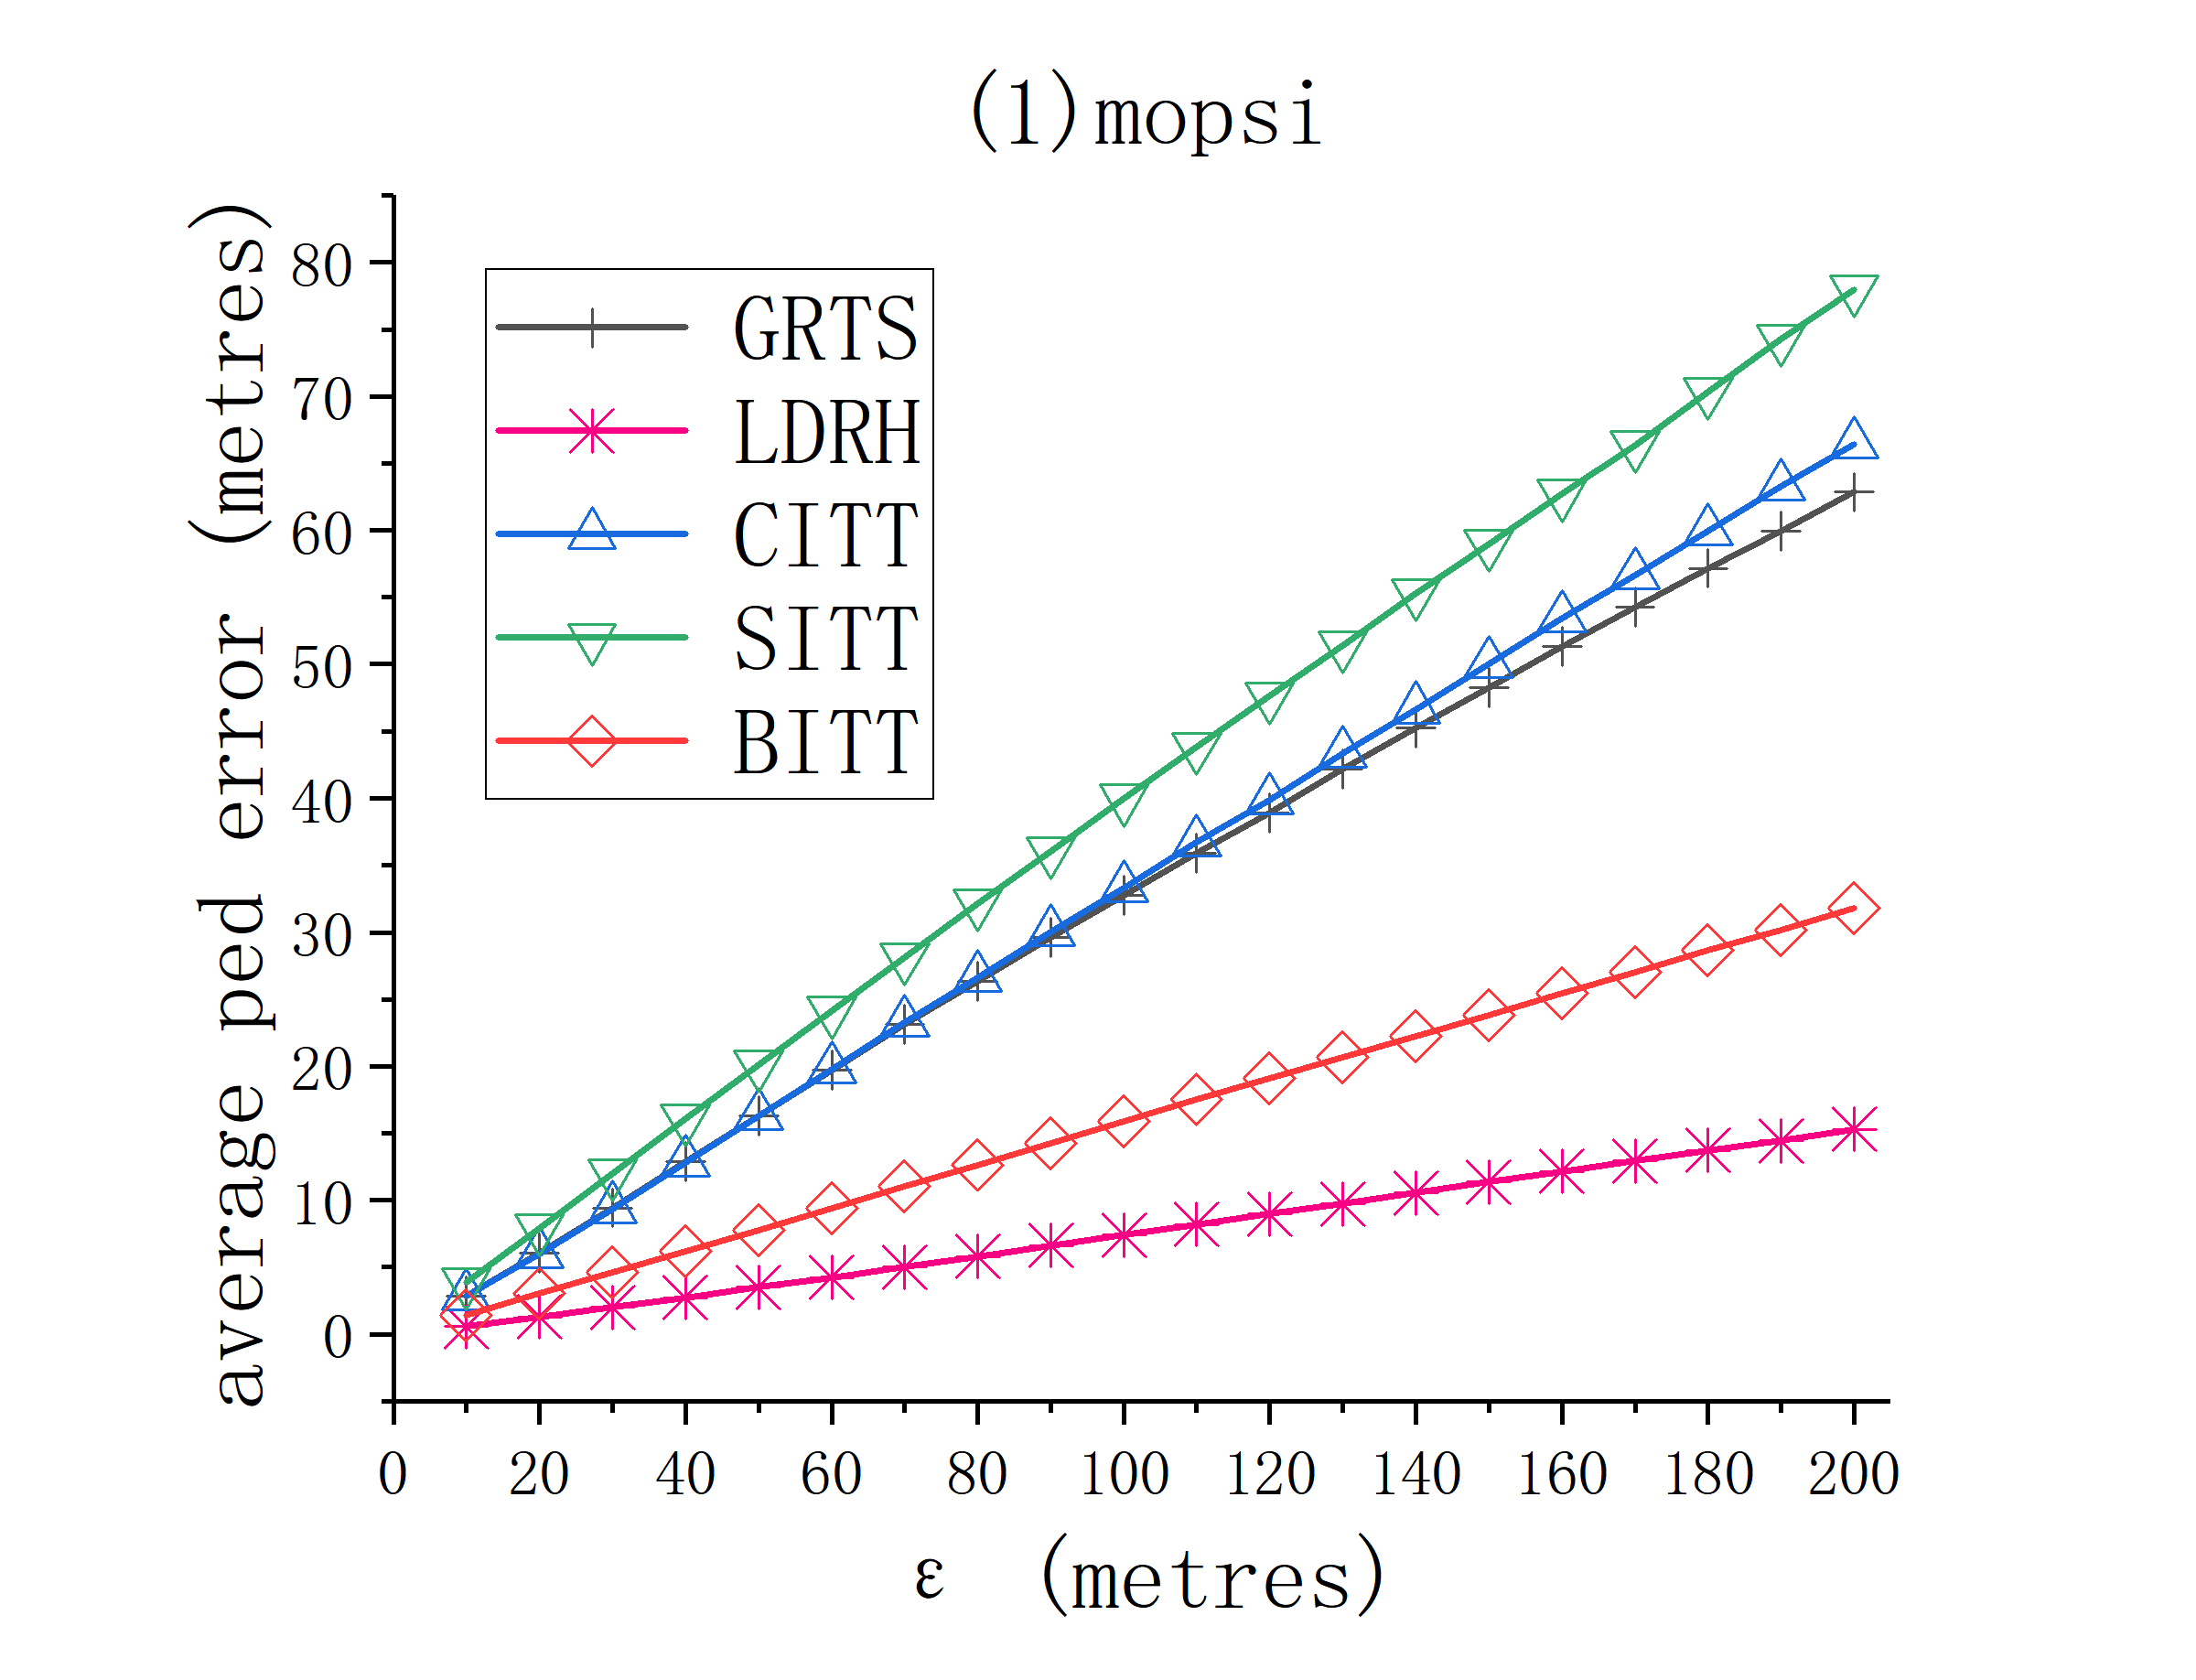
\includegraphics[scale = 0.210]{figures/Fig-mopsi-ped-error.png}\hspace{1ex}
	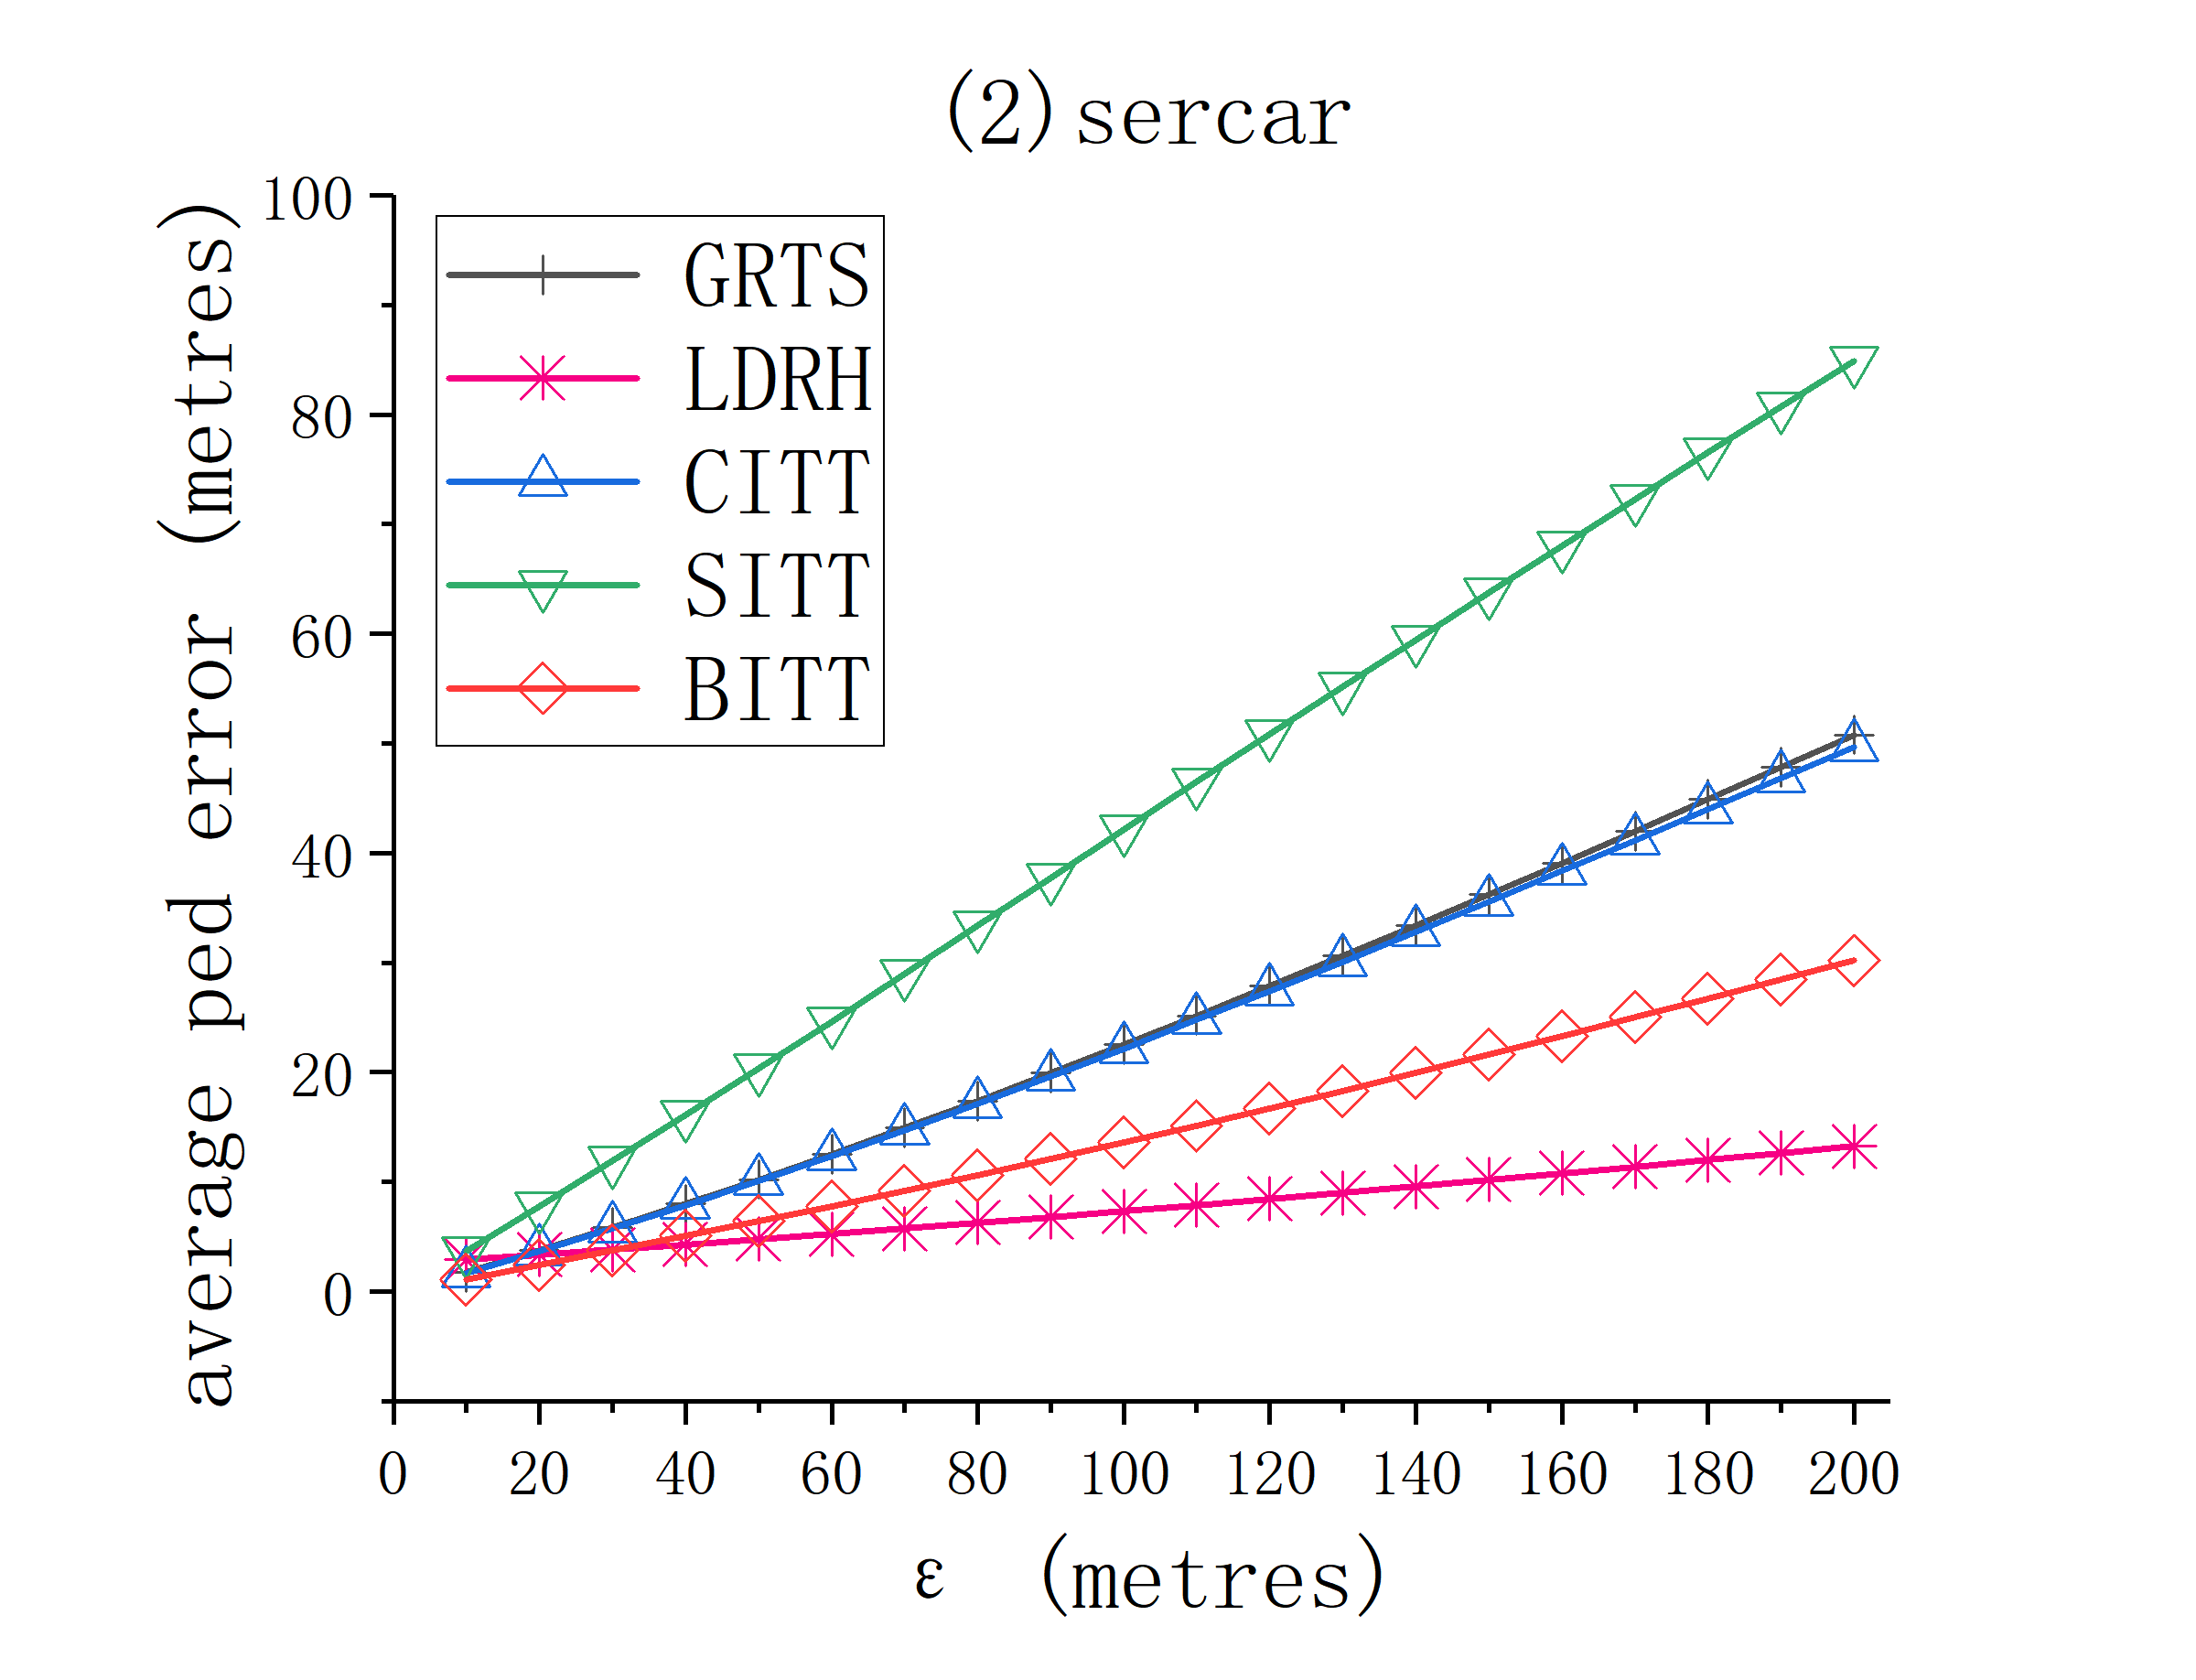
\includegraphics[scale = 0.210]{figures/Fig-sercar-ped-error.png}\hspace{1ex}
	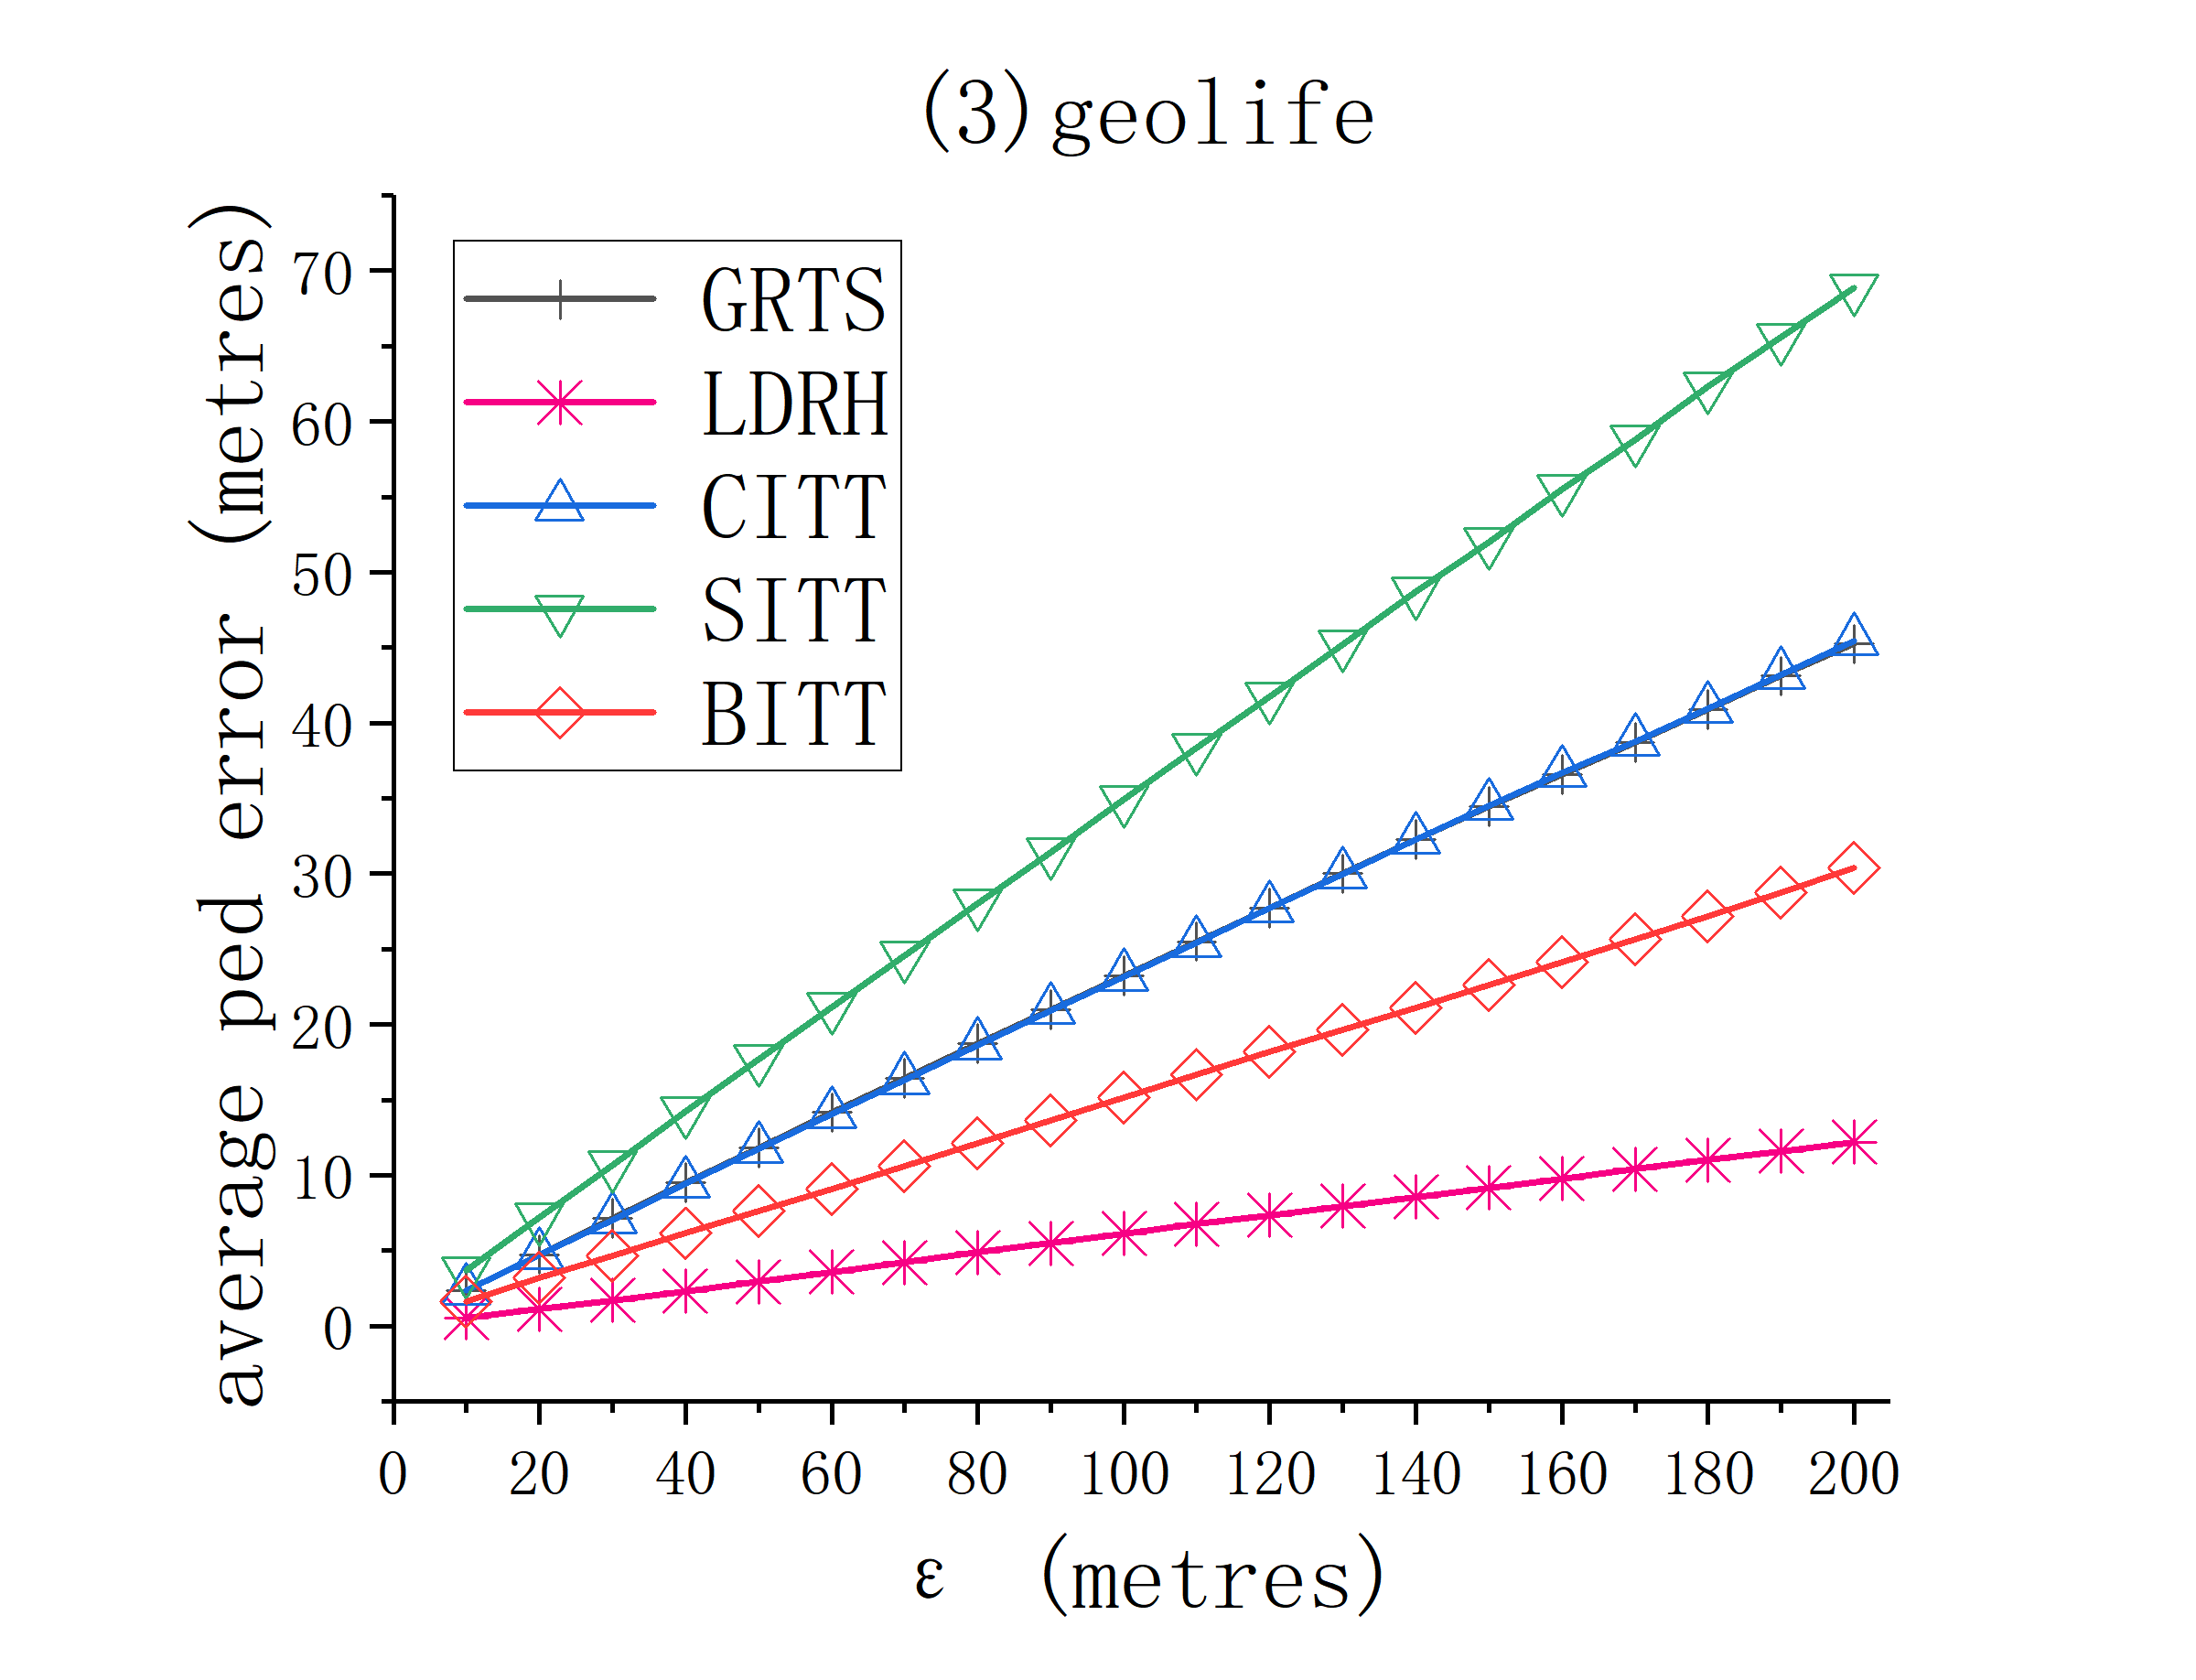
\includegraphics[scale = 0.210]{figures/Fig-geolife-ped-error.png}\hspace{1ex}
	%\vspace{-1ex}
	\caption{\small Evaluation of ped error: varying error bounds $\epsilon_{sed}$ and $\epsilon_{ped}$.}
	\label{fig:ped-error}
	%\vspace{-1ex}
\end{figure*}

\stitle{Average errors.}
%The results are reported in Figures~\ref{fig:sed-error} and Figure~\ref{fig:ped-error}.
\ni (1) Average errors increase with the increase of $\epsilon_{sed}$ and $\epsilon_{ped}$.

\ni (2) The average sed errors of these algorithms from the largest to the smallest are \sitt, \grts (\citt) and \ldrh. Among them, the average sed errors of \citt is very close to \grts.
The average sed errors of algorithms \citt and \sitt are on average
($412.7\%$, $222.8\%$, $350.1\%$)
and ($842.0\%$, $857.5\%$, $1452.5\%$)
of \ldrh and ($103.1\%$, $98.4\%$, $100.5\%$) and
($209.9\%$, $442.9\%$, $414.0\%$)
of \grts on datasets (\mopsi, \sercar, \geolife), respectively.

\ni (3) The average ped errors of these algorithms from the largest to the smallest are \sitt, \grts (\citt) and \ldrh. Among them, the average ped errors of \citt is very close to \grts.
The average ped errors of algorithms \citt and \sitt are on average
($452.2\%$, $278.1\%$, $388.9\%$)
and ($550.5\%$, $517.0\%$, $589.0\%$)
of \ldrh and ($102.0\%$, $98.3\%$, $99.7\%$) and
($123.9\%$, $187.0\%$, $150.9\%$)
of \grts on datasets (\mopsi, \sercar, \geolife), respectively.

\ni (4) The average sed errors and the average ped errors of algorithm \bitt are between \citt and \sitt.



\begin{figure*}[tb!]
	\centering
	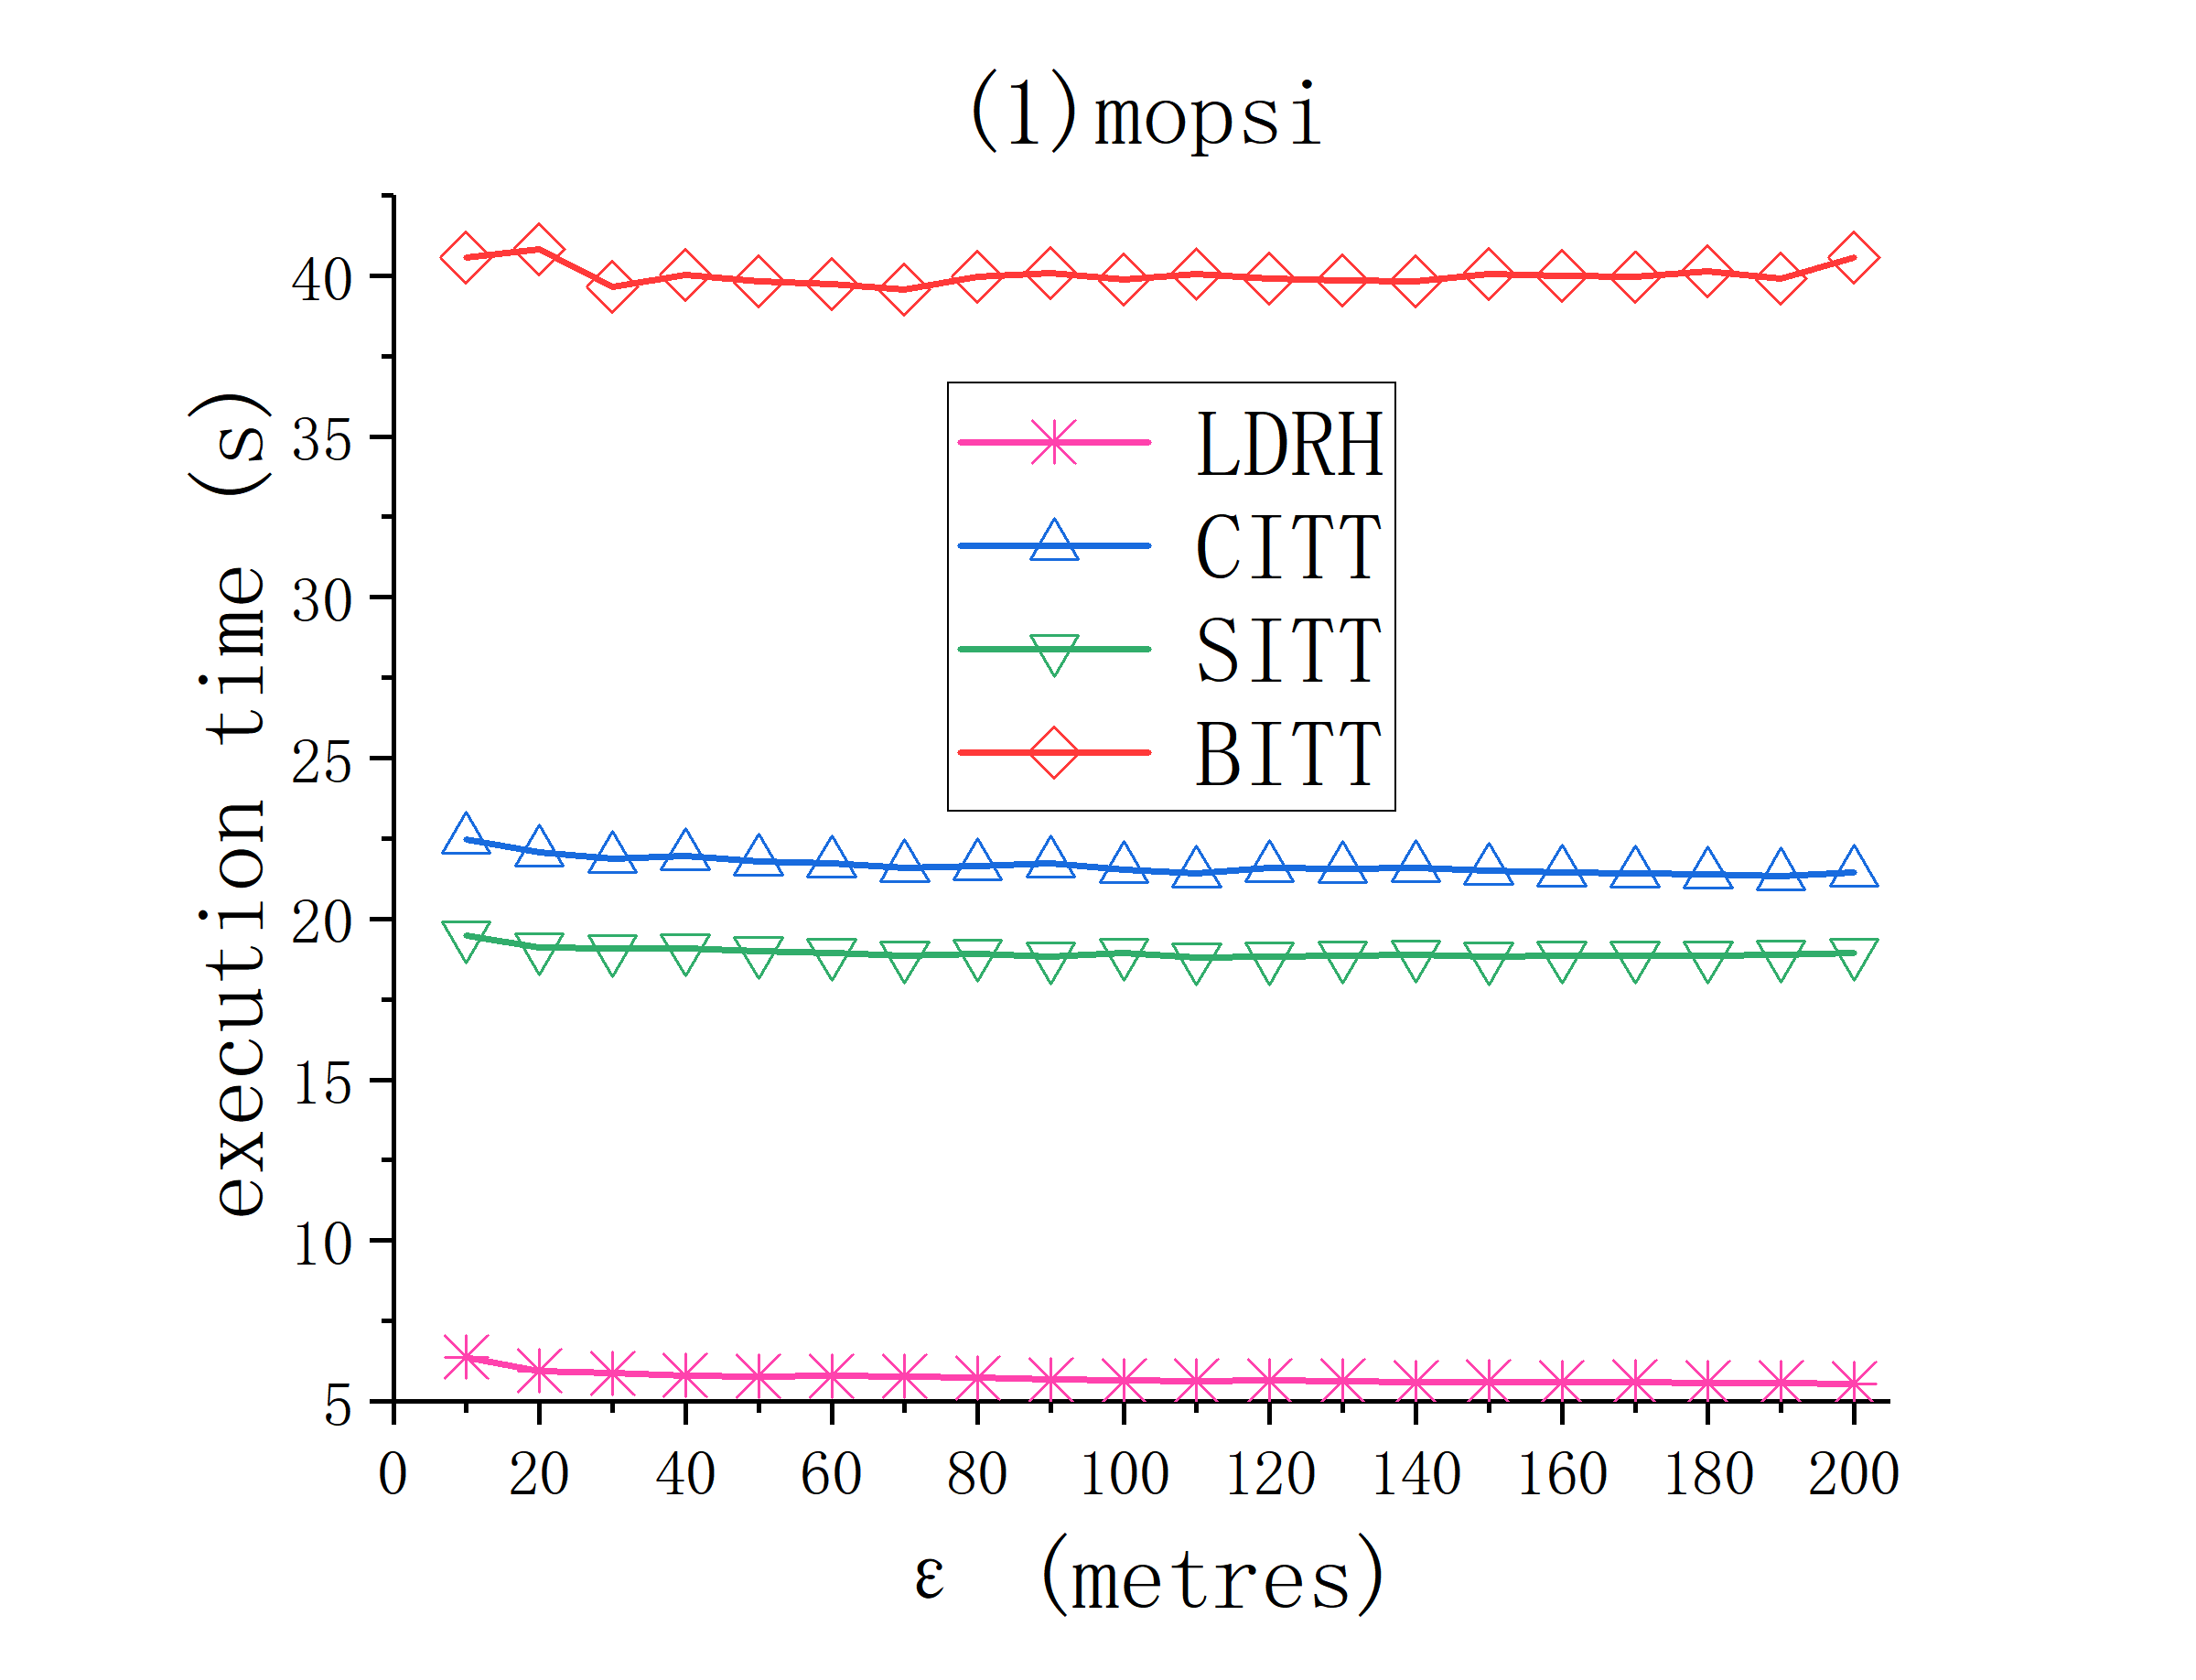
\includegraphics[scale = 0.210]{figures/Fig-mopsi-running-time.png}\hspace{1ex}
	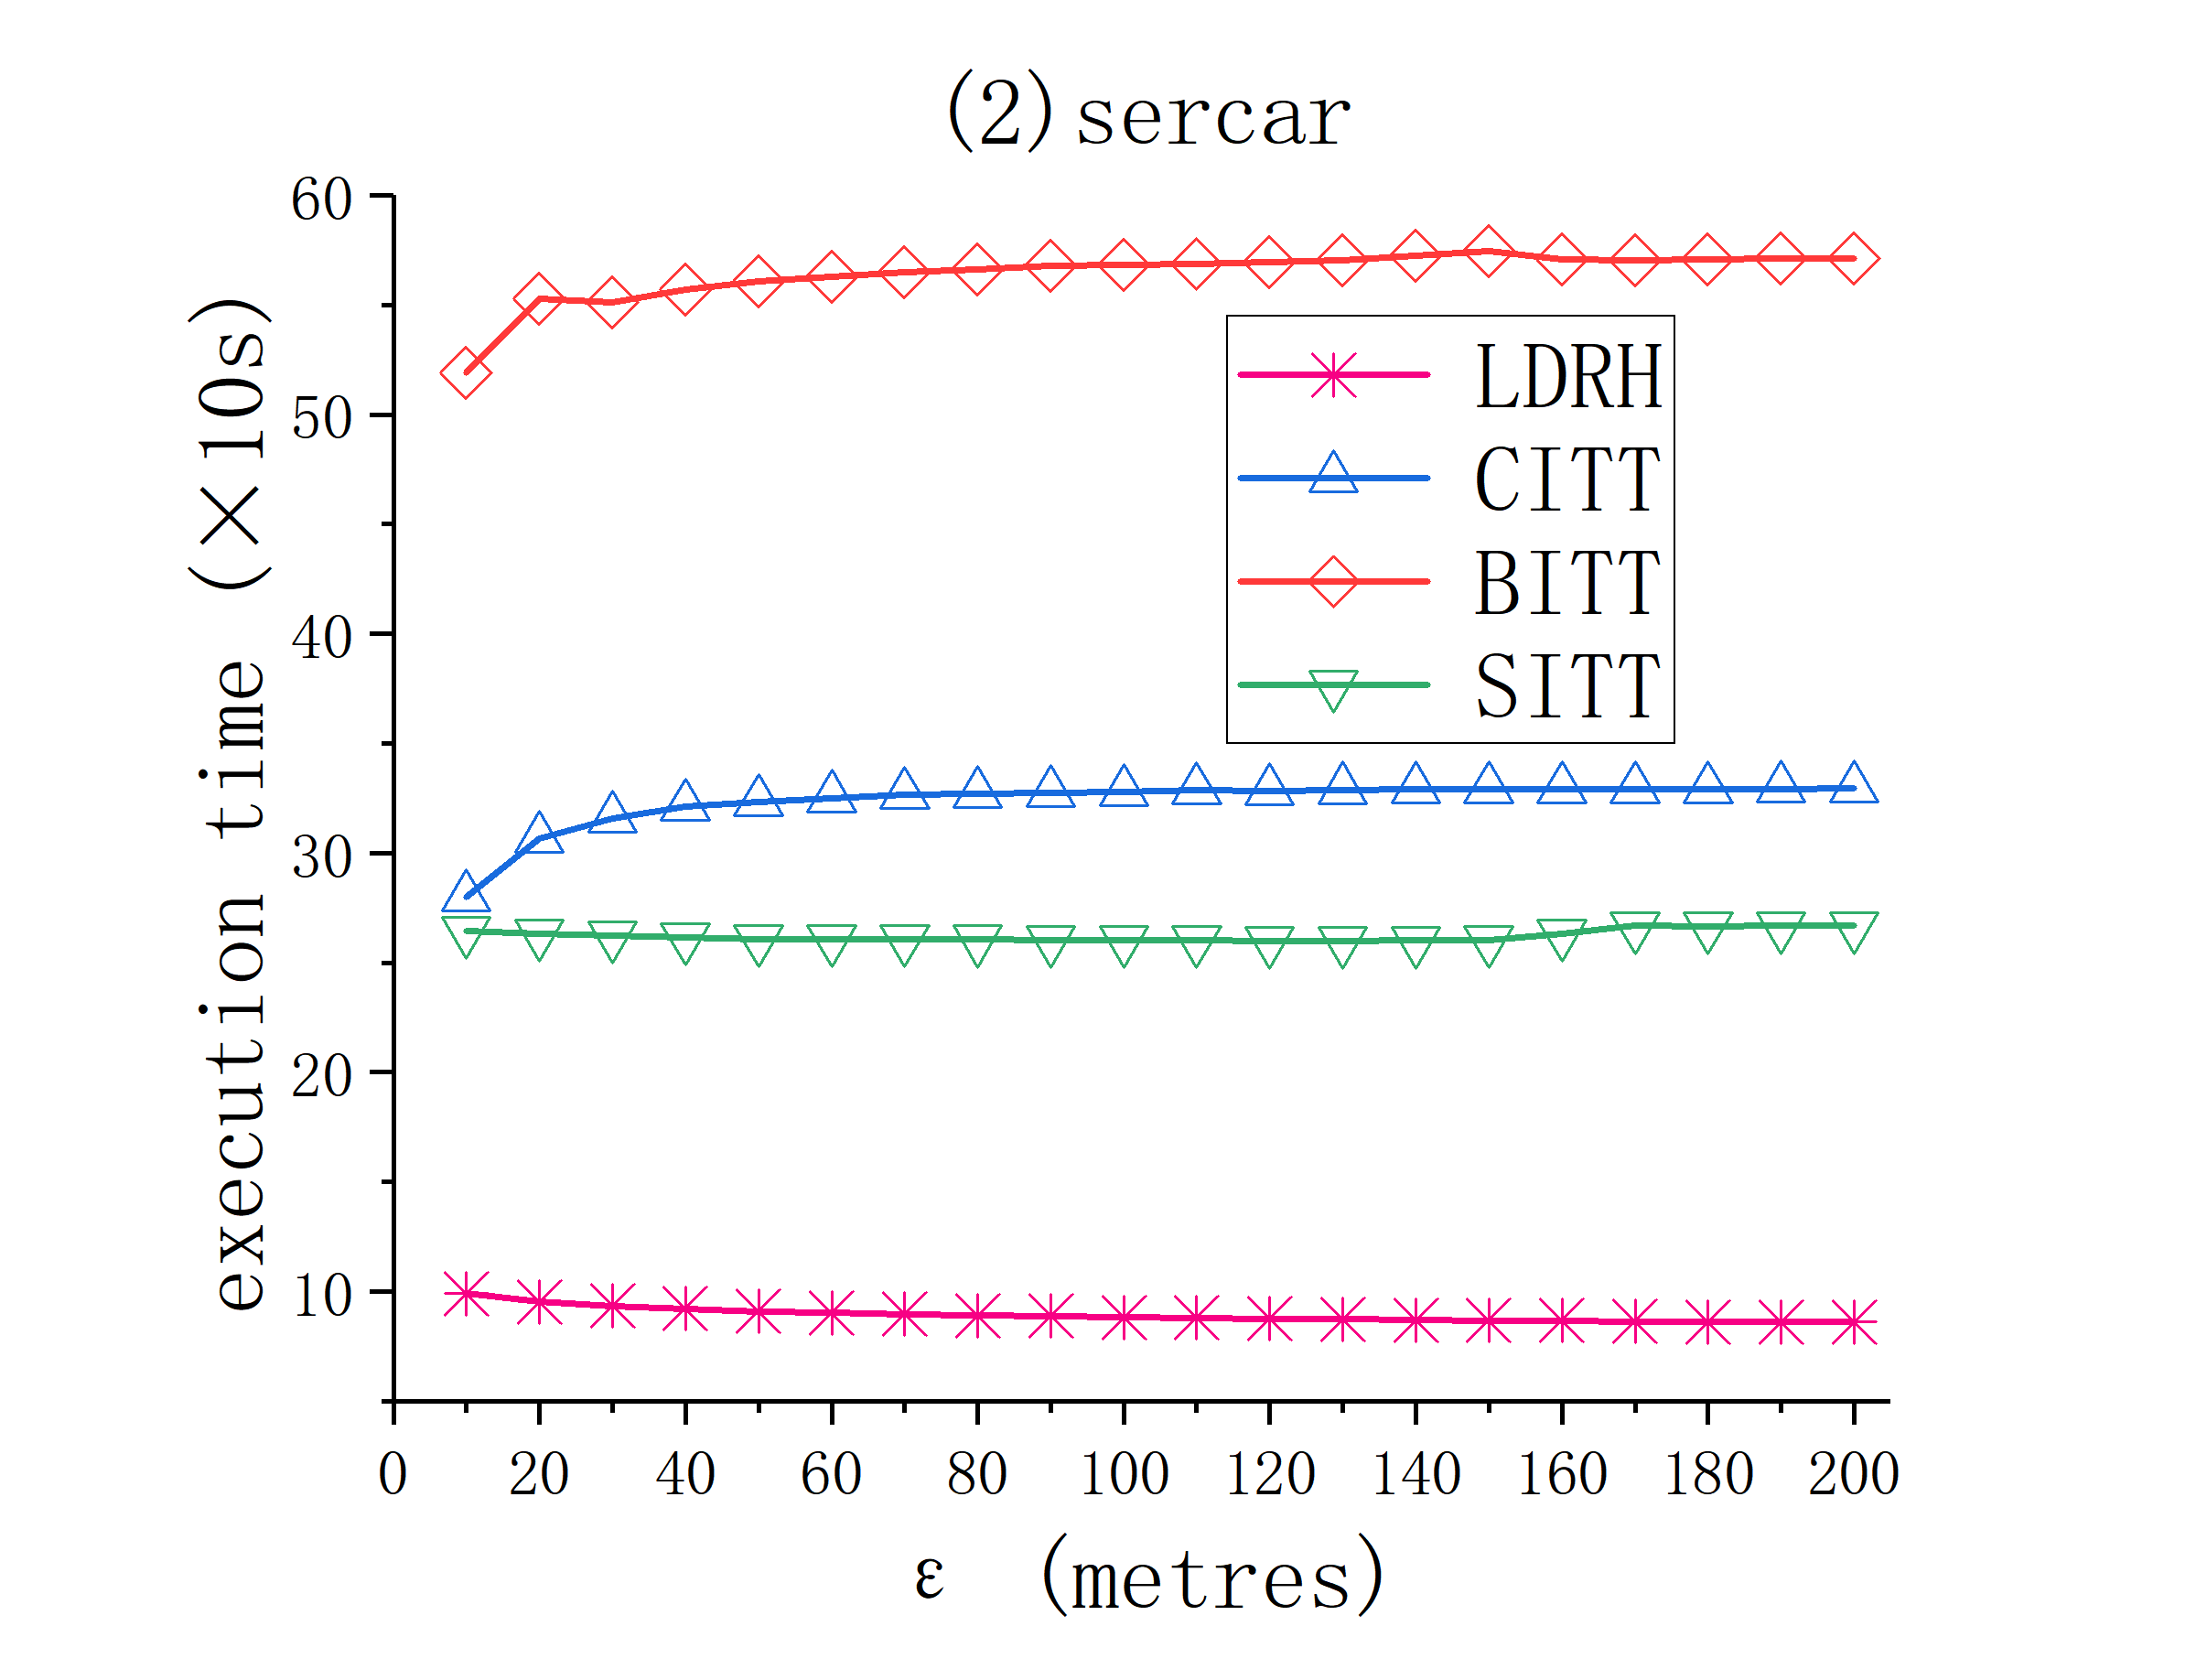
\includegraphics[scale = 0.210]{figures/Fig-sercar-running-time.png}\hspace{1ex}
	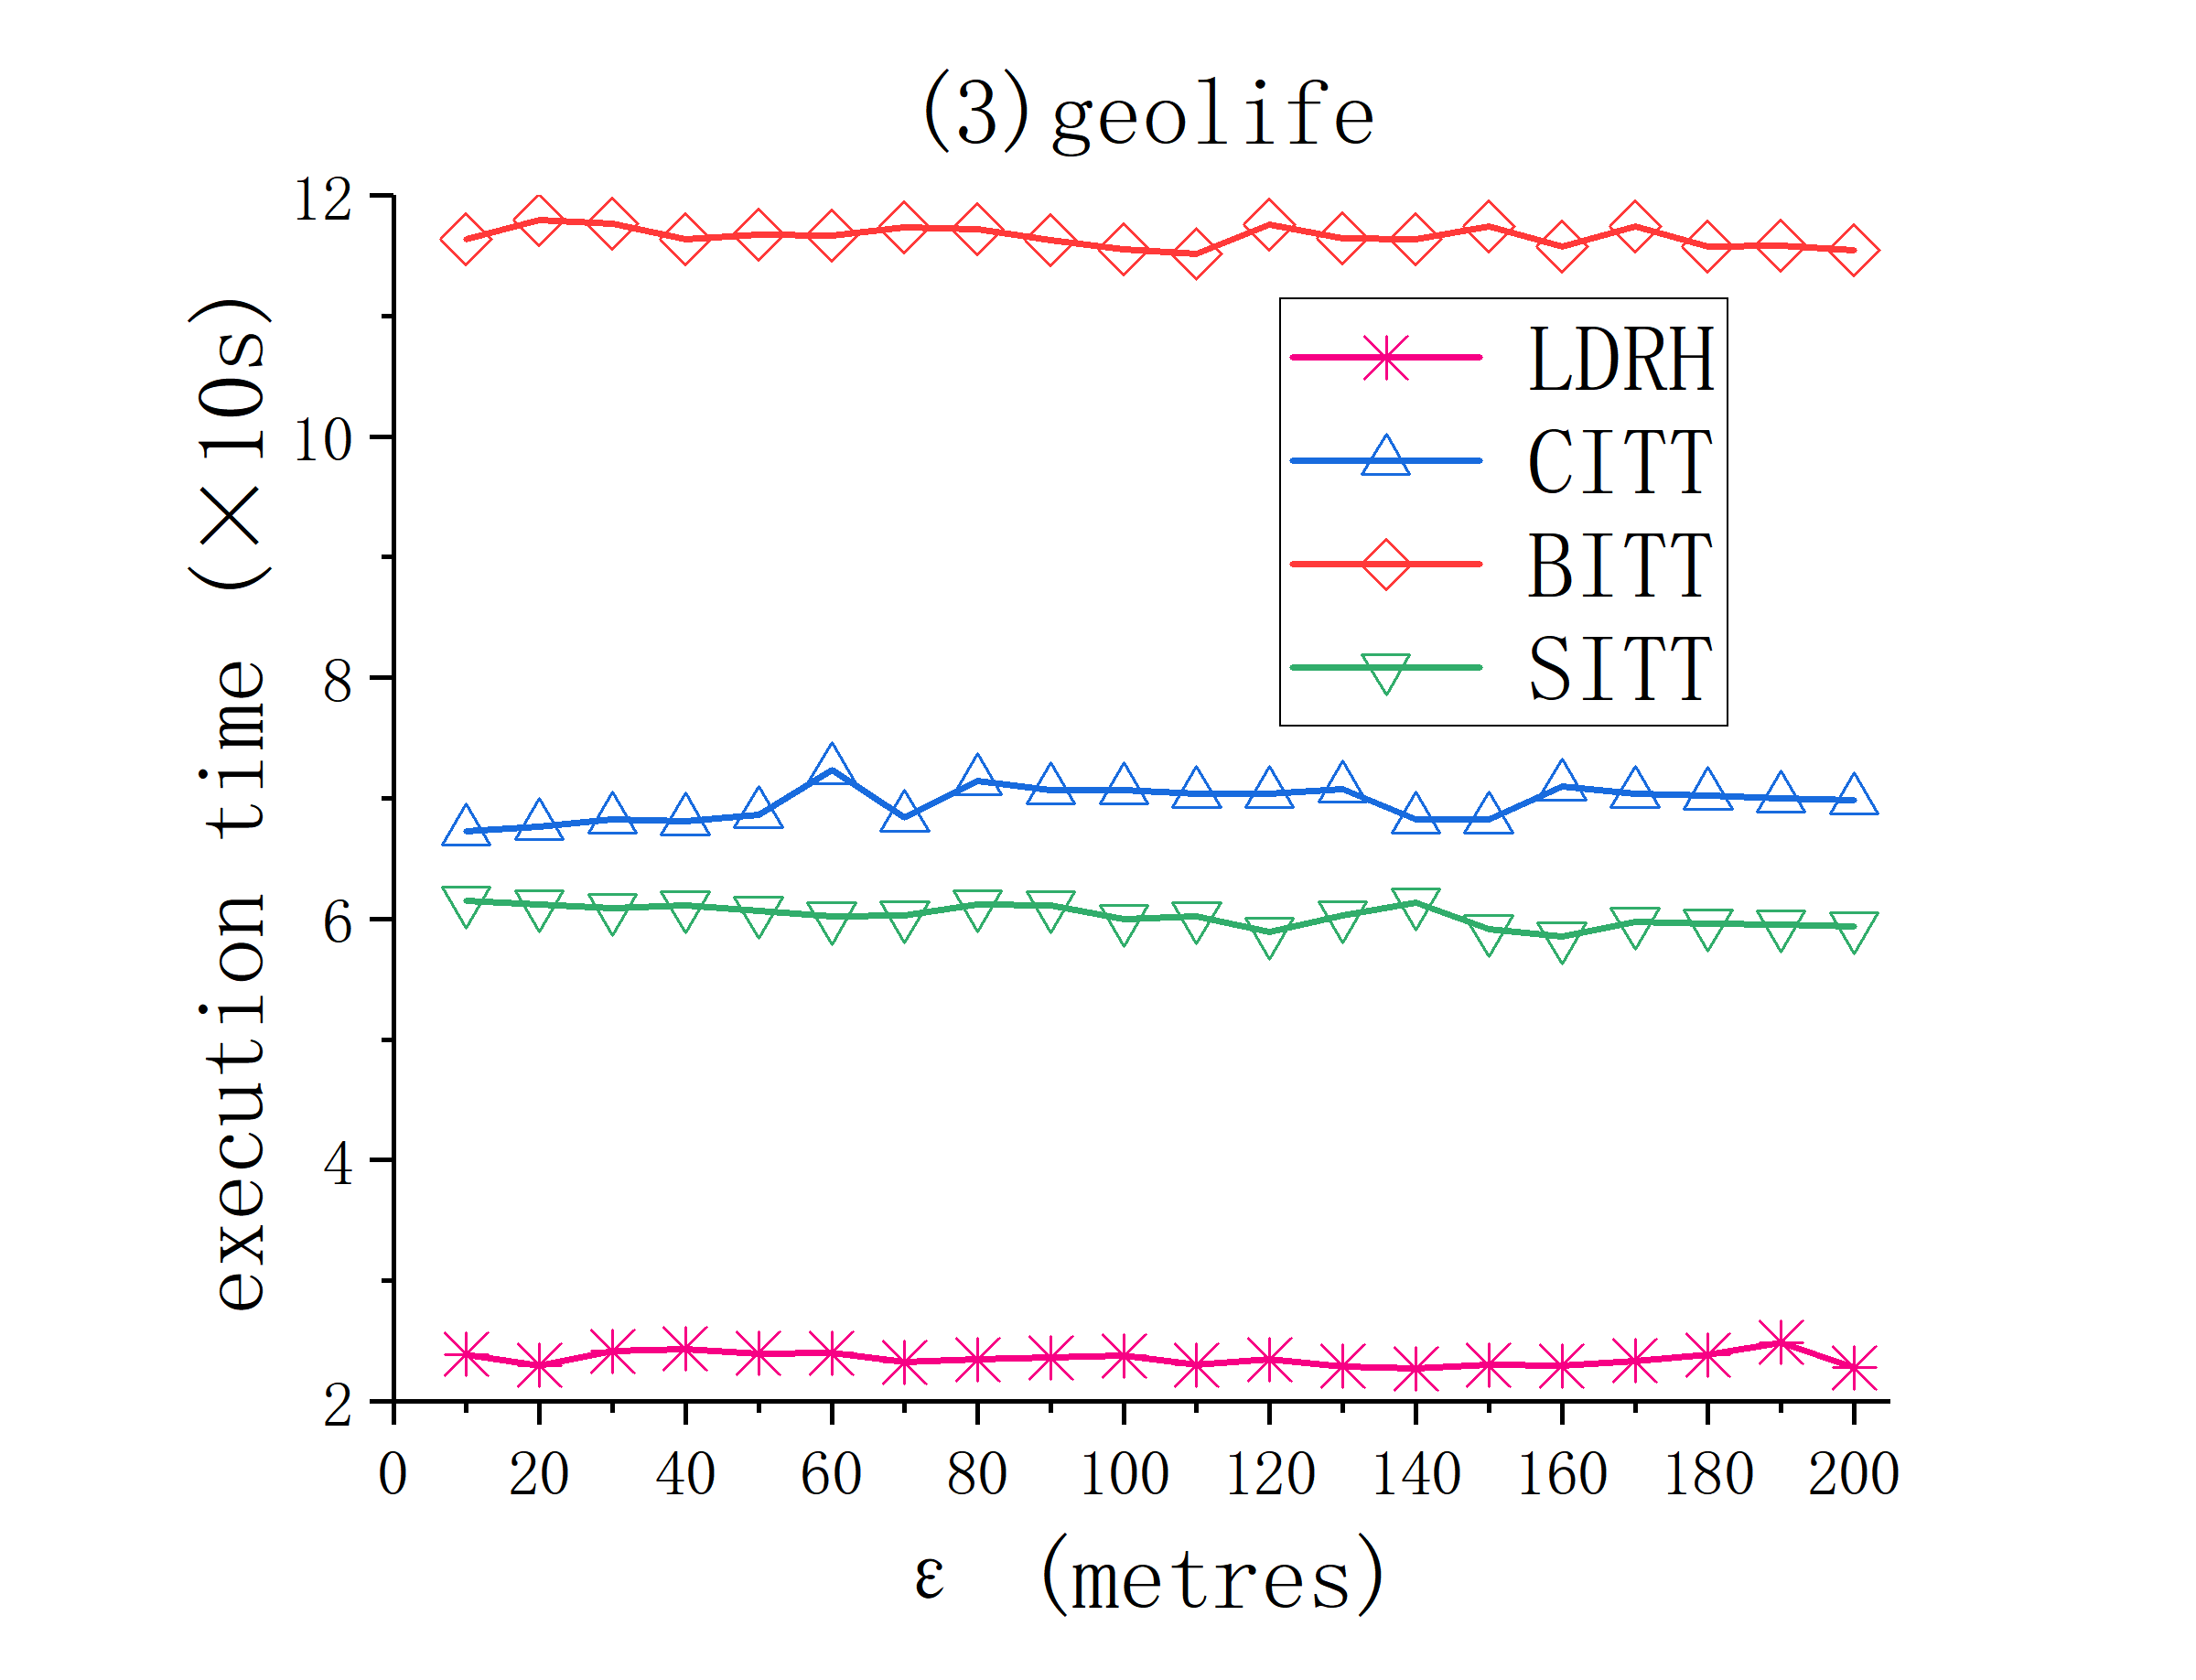
\includegraphics[scale = 0.210]{figures/Fig-geolife-running-time.png}\hspace{1ex}
	%\vspace{-1ex}
	\caption{\small Evaluation of running time: varying error bounds $\epsilon_{sed}$ and $\epsilon_{ped}$.}
	\label{fig:running-time}
	%\vspace{-1ex}
\end{figure*}

\stitle{Running time.}
%%%%%%%%%%%%%%%%% running time
%In this part of experiments, we compare the running time of our algorithms \citt, \sitt and \bitt with \ldrh and \grts.
%The results are reported in Figure~\ref{fig:running-time}. 
Since the running time of \grts is thousands of times slower than other algorithms, it is not shown in Figure~\ref{fig:running-time}.

\ni (1) The running times of these algorithms from the largest to the smallest are \grts, \bitt, \citt, \sitt and \ldrh, on all datasets.
The average running times of algorithms \citt and \sitt are on average
($378.8\%$, $363.2\%$, $296.4\%$)
and ($331.5\%$, $294.1\%$, $256.4\%$)
of \ldrh and ($0.607\%$, $21.7\%$, $0.704\%$) and
($0.529\%$, $18.1\%$, $0.623\%$)
of \grts on datasets (\mopsi, \sercar, \geolife), respectively.

\ni (2) The running time of \bitt is approximately the sum of \citt and \sitt. Because it contains the judgment conditions in \citt and \sitt.


%%% Local Variables:
%%% mode: latex
%%% TeX-master: "gis18"
%%% End:
\section{related work}
\label{sec-related}

In this section, we summarize position tracking and trajectory tracking methods. For trajectory simplification, please refer to \cite{Zhang:Evaluation, Lin:Cised} for more details.

\subsection{{Position Tracking}}

Location-aware applications, \eg car navigation or fleet management systems, need to know the current positions of moving objects. 
This location information is collected by protocols like querying protocols that pull information by the receiver and reporting protocols that push information by the sender \cite{Leonhardi:Comparison}.
The querying protocols transmit lesser data than reporting protocols at a price that they do not collect the whole trajectories of moving objects.
Paper \cite{Leonhardi:Comparison} classifies reporting protocols into simple, time-based, distance-based and dead-reckoning approaches. Among them, the dead-reckoning approach, \textcolor{blue}{\eg} LDR \cite{Wolfson:PositionTracking, Wolfson:PlainDR}, performs very well, where the update costs can be reduced by up to $85\%$ \cite{Wolfson:PositionTracking}. The current position tracking methods (\ldrh and \grts) and our methods all modify or integrate the LDR approach.

Besides, there are also road-based approaches \cite{Civilis:Techniques, Civilis:RoadTracking, Wolfson:RoadTracking} which assume that the movement of a moving object is restricted by the road network, and hence, they track the locations on roads. \cite{Wolfson:RoadTracking} is such an approach and it is reported that when the distance threshold is 0.05 miles, the performance of it is $43\%$ better than the plain LDR \cite{Wolfson:PlainDR}. 
In paper \cite{Civilis:Techniques}, the authors modified the road network and introduced acceleration on the basis of the predecessors to improve the performance of road-based position tracking.

\eat{%%%%%%%%%%%%%%%%%%
In the paper [6], the authors discussed different location tracking protocols and compared the effectiveness and efficiency of these protocols. Different location tracking algorithms are based on different metrics, for example, these algorithms can be divided into distance-based algorithms and road-based algorithms.
The representative algorithm in distance-based position tracking algorithms is LDR. In the paper [9], LDR algorithm is used to model the management of moving objects. The advantages of the LDR algorithm are simple implementation and fast processing speed. But the result of this kind of algorithm is not very good, it needs to spend a lot of network bandwidth. 
In the papers [13, 15], the authors proposed different adaptive dead reckoning algorithms. These adaptive dead reckoning algorithms improve the performance of plain dead reckoning algorithms, but there are still some efficiency problems.
Another type of algorithm is the road-based algorithm. The update policy of road-based algorithm is different from the distance-based algorithm. It assumes that the movement of the moving object is related to the road on the map and uses this to track the location. For example, in the paper [14], the authors proposed a deviation location update policy. The policy predicts that after the location is updated, the moving object will continue to move on the same street. And when the position of the moving object exceeds a given threshold from the predicted position, it will also be updated. Therefore, the algorithm ensures that the position error of the moving object is bounded. They found that when the threshold is 0.05 miles, the performance is 43\% better than the distance policy. Their algorithm assumes that map matching is always valid. If this is not the case, the algorithm will fail. In the paper [2], the authors modified the road network and introduced acceleration on the basis of the predecessors to improve the performance of the road-based algorithm.
}%%%%%%%%%%%%%%%%%%%%

\subsection{{trajectory tracking}}
\textit{Trajectory tracking} \cite{Lange:Tracking} is a combination of \textit{position tracking} \cite{Wolfson:PositionTracking,Leonhardi:Comparison} and \textit{trajectory simplification} \cite{Lin:Cised,Zhang:Evaluation}. 
%
The authors of \cite{Trajcevski:LDRH} first find that the position tracking algorithm \ldr with a small modification, \ie using a half error bound in distance checking, is also applicable to simplify the trajectory of the moving object. The modified \ldr, called \ldrh in \cite{Lange:Tracking}, is the first trajectory tracking algorithm. It is one-pass and easy to implement. However, it suffers in effectiveness in terms of compression and message ratios. 
%
\grts~\cite{Lange:GRTS,Lange:Tracking} is developed to improve the effectiveness of trajectory tracking by separating position tracking and trajectory simplification into two sub-processes such that the trajectory is buffered and effectively compressed by some existing simplification algorithm. Indeed, it introduces time and space complexities.

Both \ldrh and \grts track moving objects in floating circular shapes, while our algorithms are able to track a moving object in a floating disc, infinite beam or floating finite beam. Moreover, our algorithms like \ldrh implement position tracking and trajectory simplification in one routine. Hence, they are one-pass and efficient, and do not need any buffer. Besides, we simplify trajectories by effective approaches, \ie cone intersection and sector intersection, such that we get better effectiveness than \ldrh.


\eat{%%%%%%%%%%%%%%%%%%%%%%%
In the paper [11], the authors proposed the LDRH algorithm. This algorithm modifies the LDR algorithm and makes it applicable to trajectory tracking. The LDRH algorithm is a one-pass algorithm with good running speed, but the compression effect is not ideal.
Another representative trajectory tracking algorithm is GRTS[4, 5]. GRTS has good compression ratio, and can be used in combination with different compression algorithms to directly balance the computational cost and compression ratio. But the GRTS algorithm has certain disadvantages: 1. GRTS algorithm requires a buffer, which brings storage limitations. 2. GRTS separates compression and position tracking. 

why not integrate one-pass algorithms with GRTS? 1. One pass algorithm does not need a buffer, but GRTS requires a buffer. 2. A one-pass algorithm runs in a manner similar with LDR, which inspires us to develop effective and efficient trajectory tracking methods that combine compression and position tracking into a consistent algorithm, and run in one-pass manner.
}%%%%%%%%%%%%%%%%%%%%%%%%%




%%% Local Variables:
%%% mode: latex
%%% TeX-master: "gis18"
%%% End:
\section{conclusion}
\label{sec-conclusion}

We have provided a way to design a rectangle-like shape, and developed a one-pass trajectory tracking algorithm \bitt and its variations \citt and \sitt to effectively and efficiently track a moving object in rectangle-like, circular and strip areas, respectively.
We have also experimentally evaluated the performance of our algorithms compared with two representative trajectory tracking algorithms \ldrh (the most efficient) and \grts (currently the most effective). 
They are tens of times faster than \grts and several times slower than \ldrh.
In terms of compression and message ratios, \bitt, \citt and \sitt send fewer messages than \grts and \ldrh, and have the similar compression ratios compared with \grts.
%\sitt (using \ped) outperforms \grts in both metrics.

%\todo{different position and traj errors? combination of distance metrics}
%\section*{{Appendix:  Proofs}}





\stitle{Proof of Theorem~\ref{theo-ldrh-cised}}:
If $\dddot{\mathcal{T}}_s$ can be represented by line segment $\overline{P_sP_{s+k}}$ by algorithm \ldrh, then we have $|P_{s+i}P'_{s+i}| < \epsilon/2$ for each $i \in (0, k)$, where $P'_{s+i}$ is the expected position (synchronized point) of $P_{s+i}$ \wrt the initial velocity $\vv{v}$ of \ldrh.
From the view of the ``x-y-t" 3D space, $\vv{v}$ must be in the common intersection of  $\bigsqcap_{i=1}^{k}$\cone{(P_s, P_{s+i}, \epsilon/2)}, in other words, we have $\bigsqcap_{i=1}^{k}$\cone{(P_s, P_{s+i}, \epsilon/2)} $\ne \{P_s\}$, meaning this sub-trajectory can be represented by approaches based on the spatio-temporal cones.
\eop

\stitle{Proof of Theorem~\ref{theo-full-cone}}:
Let $P'_{s+i}$ be the intersection point of line segment $\overline{P_sP_{s+k}}$ and plane $t = P_{s+i}.t,~i\in (0,k)$, indeed, $P_{s+i}$ is the synchronized point of $P_{s+i}$ \wrt line segment $\overline{P_sP_{s+k}}$. 
Because $\overline{P_sP_{s+k}}$ passes through $\bigsqcap_{i=1}^{k-1}$\cone{(P_s, P_{s+i}, \epsilon)} - \{$P_s$\}, $P'_{s+i}$ must be inside of the synchronous circle of $P_{s+i}$ on the plane. Thus we have $|P_{s+i}P'_{s+i}|<\epsilon$, \ie $sed(P_{s+i}, \overline{P_sP_{s+k}})|<\epsilon$.
\eop

\stitle{Proof of Theorem~\ref{theo-cone-vs}}:
(1) If $\bigsqcap_{i=1}^{k}$\cone{(P_s, P_{s+i}, \epsilon/2)} $\ne \{P_s\}$, then $sed(P_{s+i}, P_sP_{s+k}) <\epsilon$ for each $i \in [1,k]$. 
The intersection point  $P'_{s+i}$ of line segment $P_s P_{s+k}$ and plane $t = P_{s+i}.t$ is the synchronized point of $P_{s+i}$ \wrt $P_s P_{s+k}$, such that $|P_{s+i}P'_{s+i]}| < \epsilon$. Hence for each $i \in [1,k]$, $P'_{s+i}$ falls in the synchronous circle of $P_{s+i}$ on the plane, meaning $\overline{P_sP_{s+k}}$ passes through the common intersection of the preview cones $\bigsqcap_{i=1}^{k-1}$\cone{(P_s, P_{s+i}, \epsilon)}-$\{P_s\}$.
%
(2) If line segment $\overline{P_sP_{s+k}}$ passes through the common intersection $\bigsqcap_{i=1}^{k-1}$\cone{(P_s, P_{s+i}, \epsilon)} - \{$P_s$\}, then, suppose there is $i$ and $j$ ($i<j<k$) such that $P^{s+j}_{s+i}$ and $P^{s+k}_{s+i}$ are the intersection points of $\overline{P_sP_{s+j}}$ and $\overline{P_sP_{s+k}}$ with the plane $t = P_{s+i}.t$, respectively, we have $0 \le |P_{s+i}P^{s+k}_{s+i}|<\epsilon$ and $0 \le |P^{s+j}_{s+i}P^{s+k}_{s+i}|<\epsilon$, meaning $0 \le |P_{s+i}P^{s+j}_{s+i}|<2\epsilon$, \ie~$|P_{s+i}P^{s+j}_{s+i}|$ is not necessarily less than $\epsilon$. 
%
If it is greater than $\epsilon$, then the intersection of \cone{(P_s,P_{s+i},\epsilon/2)} and \cone{(P_s,P_{s+j},\epsilon/2)} is $\{P_s\}$, and $\bigsqcap_{i=1}^{k}$\cone{(P_s, P_{s+i}, \epsilon/2)} is also $\{P_s\}$.
%
Combine (1) and (2) we have the conclusion.
\eop

\stitle{Proof of Theorem~\ref{theo-half-sector}}:
Trajectory tracking is the combination of trajectory simplification and position tracking.
%
(1) Trajectory simplification: It can be simplified in strip-like areas as shown in Section \ref{sec:sector-in-simp};
%
(2) Position tracking: If it can be represented by a line segment by the intersection of sectors, then there is sure a $\vv{v}$ living in the common intersection of sectors, \eg $\vv{v}$ on $P_sP_{s+i}$, such that it is applicable to track the position in strip areas.
%
Combine (1) and (2), we have the conclusion.
\eop


\stitle{{Proof of Theorem~\ref{theo-full-sector}}}:
First, let $|P_sP_{s+k}| = \sqrt{l_m^2 - \epsilon^2}$. We draw an arc $\widehat{BD}$ taking $P_s$ as its center and $l_m$ as its radius, and two lines $\overline{AB}$ and $\overline{CD}$ paralleling and having a distance of $\epsilon$ to $\overline{P_sP_{s+k}}$, as shown in Figure \ref{fig:sectorinter}.
Because line segment $\overline{P_sP_{s+k}}$ passes through $\bigsqcap_{i=1}^{k-1}$\sector{(P_s, P_{s+j}, \epsilon)}- $\{P_s\}$ and $l_{m} = max\{|P_sP_{s+i}|\}$ for each $i \in (0, k)$, point $P_{s+i}$ must live in the area between lines $\overline{AB}$ and $\overline{CD}$, and in the inner side of arc $\widehat{BD}$.
(1) If $P_{s+i}$ is between $\overline{BD}$ and $\widehat{BD}$, then $ped(P_{s+i}, \overline{P_sP_{s+k}}) = |{P_{s+i}P_{s+k}}| < |{BP_{s+k}}| = \epsilon$; 
(2) If $P_{s+i}$ is in the left side of $\overline{BD}$, then  $ped(P_{s+i}, \overline{P_sP_{s+k}})$ is the perpendicular Euclidean distance from $P_{s+i}$ to the line segment $\overline{P_sP_{s+k}}$ that is also less than $\epsilon$. Combining (1) and (2) we have $ped(P_{s+i}, \overline{P_sP_{s+k}})< \epsilon$ for $|P_sP_{s+k}| = \sqrt{l_m^2 - \epsilon^2}$.
Next, it is easy to find that if $|P_sP_{s+k}| > \sqrt{l_m^2 - \epsilon^2}$ then the conclusion remains the same.
%then for each point $P_{s+i}$, $i\in (0,k)$, it has a Euclidean distance $d_i$ less than $\epsilon$ to the line that $\overline{P_sP_{s+k}}$ lives on. We also know that $\overline{P_sP_{s+k}}$ is not shorter than any other line segment, thus, the distance $d_i$ is indeed the \ped of $P_{s+i}$ to the line segment $\overline{P_sP_{s+k}}$. That is, $ped(P_{s+i}, P_sP_{s+k}) <\epsilon$ for each $i\in (0,k)$.
\eop

\begin{figure}[tb!]
	\centering
	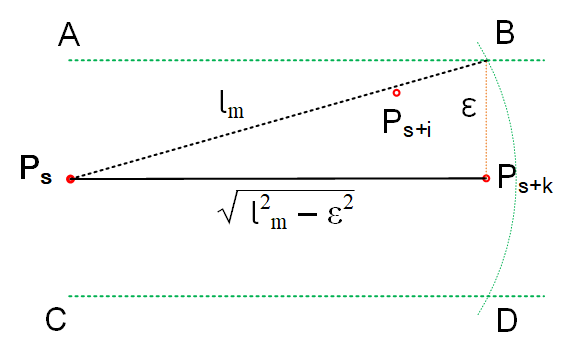
\includegraphics[scale=1.0]{figures/Fig-SectorInter.png}
	\vspace{-2ex}
	\caption{\small The intersection of full-$\epsilon$ sectors.  }
	\vspace{-1ex}
	\label{fig:sectorinter}
\end{figure}

\eat{%%%%%%%%%%%%%%%%%%%%%%%%%%%%%%%%%%
\stitle{\textcolor{red}{Proof of Theorem~\ref{theo-full-sector}}}:
If line segment $\overline{P_sP_{s+k}}$ passes through $\bigsqcap_{i=1}^{k-1}$\sector{(P_s, P_{s+j}, \epsilon)}- $\{P_s\}$, \ie it lives in all the preview sectors, then for each point $P_{s+i}$, $i\in (0,k)$, it has a Euclidean distance $d_i$ less than $\epsilon$ to the line that $\overline{P_sP_{s+k}}$ lives on. We also know that $\overline{P_sP_{s+k}}$ is not shorter than any other line segment, thus, the distance $d_i$ is indeed the \ped of $P_{s+i}$ to the line segment $\overline{P_sP_{s+k}}$. That is, $ped(P_{s+i}, P_sP_{s+k}) <\epsilon$ for each $i\in (0,k)$.
\eop

\stitle{Proof of Theorem~\ref{theo-sector-vs}}:
(1) If $\bigsqcap_{i=1}^{k}$\sector{(P_s, P_{s+i}, \epsilon/2)} $\ne \{P_s\}$, then $\overline{P_sP_{s+k}}$ lives in the common intersection of the preview half-$\epsilon$ sectors. 
Hence, it is sure living in the common intersection of the preview full-$\epsilon$ sectors, \ie it passes through $\bigsqcap_{i=1}^{k-1}$\sector{(P_s, P_{s+i}, \epsilon)} $- \{P_s\}$.
%
(2) If line segment $\overline{P_sP_{s+k}}$ passes through the common intersection $\bigsqcap_{i=1}^{k-1}$\sector{(P_s, P_{s+i}, \epsilon)} - \{$P_s$\}, then, given $i$ and $j$ ($i<j<k$), it is possible that $ped(P_{s+i}, \overline{P_sP_{s+k}})> \epsilon/2$ and $ped(P_{s+j}, \overline{P_sP_{s+k}})> \epsilon/2$ , meaning the intersection of \sector{(P_s,P_{s+i},\epsilon/2)} and \sector{(P_s,P_{s+j},\epsilon/2)} is $\{P_s\}$, and thus, $\bigsqcap_{i=1}^{k}$\sector{(P_s, P_{s+i}, \epsilon/2)} is also $\{P_s\}$.
%
Combine (1) and (2) we have the conclusion.
\eop
}%%%%%%%%%%%%%%%%%%%%%%%%%%%%%%%%%%%%%

\stitle{Proof of Theorem~\ref{theo-binary}}:
Given a sub-trajectory $[P_s,...,P_{s+k}]$ and two error bounds $\epsilon_{sed}$ and $\epsilon_{ped}$ satisfying $\epsilon_{sed} > \epsilon_{ped}$, from Theorems~\ref{theo-ldrh-cised} and \ref{theo-half-sector}, we know this sub-trajectory can be tracked in a circular and a strip areas, respectively.  
%
(1) Trajectory simplification: Let $\overline{P_sP_{s+i}}, i\in (0,k],$ be the line segment representing sub-trajectory $[P_s,...,P_{s+i}]$, because $\epsilon_{sed} > \epsilon_{ped}$, these areas indeed form a rectangle-like area, \ie this sub-trajectory can be simplified in rectangle-like areas by combining sectors and spatio-temporal cones.
%
(2) Position tracking: If the sub-trajectory $[P_s,...,P_{s+i}]$ can be represented by line segment $\overline{P_sP_{s+i}}$ by the intersections of sectors and cones, then there is sure a velocity $\vv{v}$ living in the common intersections of cones and sectors, such that it is applicable to track the position of the moving object in a rectangular-like area \wrt the $P_s$ and $\vec{v}$. 
Combine (1) and (2) we have the conclusion.
\eop




\eat{
	\section*{Acknowledgments}
	This work is supported in part by NSFC (U1636210), NSFC ({61421003}) and Beijing Advanced Innovation Center for Big Data and Brain Computing.
}

\balance
\bibliographystyle{ACM-Reference-Format}
\bibliography{ref-traj-simp}

\end{document}
